% ************************************************************************* %
%DIF LATEXDIFF DIFFERENCE FILE
%DIF DEL C:\Users\ssingh\Documents\GitHub\template_to_latex\overleaf\v1.4\MTConnect Part 2\main.tex   Tue Jul 16 07:42:51 2019
%DIF ADD C:\Users\ssingh\Documents\GitHub\template_to_latex\overleaf\v1.5\MTConnect Part 2\main.tex   Tue Jul 16 07:42:51 2019
% ********************** MTCONNECT DOCUMENT TEMPLATE ********************** %
% ************************************************************************* %
% 	FILENAME: 		mtconnect.tex											%
%	VERSION:		0.1														%
% 	DATE:			02/13/2018												%
%	PORTED BY:		Moneer Helu												%
%	ADDRESS:		Engineering Laboratory									%
%					National Institute of Standards and Technology (NIST)	%
%					100 Bureau Drive										%
%					Mailstop 8260											%
%					Gaithersburg, MD 20899									%5
%					United States of America								%
% 	EMAIL:			moneer.helu@nist.gov									%
% 	DESCRIPTION:	Template for MTConnect documentation;					%
% 					Initial attempt for testing and discussion				%
% 	USAGE:			\documentclass[options]{mtconnect}						%
% ************************************************************************* %

\documentclass{mtconnect}	% Load mtconnect document class

% \newacronym[longplural={Frames per Second}]{tag}{ABRV}{Description}
\newacronym[longplural={application programming interfaces}]{api}{API}{application programming interface}
\newacronym[longplural={bills of materials}]{bom}{BOM}{bill of materials}
\newacronym[longplural={designated-engineering representatives}]{der}{DER}{designated-engineering representative}
\newacronym[longplural={digital manufacturing certificates}]{dmc}{DMC}{digital manufacturing certificate}
\newacronym[longplural={small-to-medium enterprises}]{sme}{SME}{small-to-medium enterprise}
%\newacronym[longplural={Uniform Resource Identifiers}]{uri}{URI}{Uniform Resource Identifier}
\newacronym{2d}{2D}{two-dimensional}
\newacronym{3d}{3D}{three-dimensional}
\newacronym{ai}{AI}{artificial intelligence}
\newacronym{alm}{ALM}{application lifecycle management}
\newacronym{amt}{AMT}{The Association for Manufacturing Technology}
\newacronym{ansi}{ANSI}{American National Standards Institute}
\newacronym{ap}{AP}{Application Protocol}
\newacronym{asme}{ASME}{American Society of Mechanical Engineers}
\newacronym{astm}{ASTM}{American Society for Testing and Materials}
\newacronym{aws}{AWS}{American Welding Society}
\newacronym{bdd}{BDD}{block definition diagram}
\newacronym{bst}{BST}{Board on Standardization and Testing}
\newacronym{ca}{CA}{certificate authority}
\newacronym{cad}{CAD}{computer-aided design}
\newacronym{cae}{CAE}{computer-aided engineering}
\newacronym{cai}{CAI}{computer-aided inspection}
\newacronym{cam}{CAM}{computer-aided manufacturing}
\newacronym{cax}{CAx}{computer-aided technologies}
\newacronym{cfd}{CFD}{computational fluid dynamics}
\newacronym{cm}{CM}{configuration management}
\newacronym{cms}{CMS}{coordinate-measurement system}
\newacronym{cnri}{CNRI}{Corporation for National Research Initiatives}
\newacronym{cpm}{CPM}{Core Product Model}
\newacronym{cpm2}{CPM2}{Revised Core Product Model}
\newacronym{cpsc}{CPSC}{Consumer Product Safety Commission}
\newacronym{cr}{C\&R}{cause and remedy}
\newacronym{cuav}{cUAV}{configurable unmanned aerial vehicle}
\newacronym{darpa}{DARPA}{Defense Advanced Research Projects Agency}
\newacronym{dfm}{DFM}{design for manufacturing}
\newacronym{dla}{DLA}{Defense Logistics Agency}
\newacronym{dmsc}{DMSC}{Dimensional Metrology Standards Consortium}
\newacronym{dns}{DNS}{Domain Name System}
\newacronym{dod}{DoD}{U.S. Department of Defense}
\newacronym{doi}{DOI}{Distributed Object Identifier}
\newacronym{drm}{DRM}{digital rights management}
\newacronym{ecr}{ECR}{engineering change request}
\newacronym{erp}{ERP}{enterprise resource planning}
\newacronym{faa}{FAA}{Federal Aviation Administration}
\newacronym{fair}{FAIR}{first article inspection reporting}
\newacronym{fda}{FDA}{Food and Drug Administration}
\newacronym{fea}{FEA}{finite-element analysis}
\newacronym{gdt}{GD\&T}{geometric dimensions and tolerances}
\newacronym{gid}{GID}{global identifier}
\newacronym{html}{HTML}{Hypertext Markup Language}
%\newacronym{http}{HTTP}{Hypertext Transfer Protocol}
\newacronym{https}{HTTPS}{Hypertext Transfer Protocol over Secure Sockets Layer}
\newacronym{ieee}{IEEE}{Institute of Electrical and Electronics Engineers}
\newacronym{iiot}{IIoT}{industrial internet of things}
\newacronym{incose}{INCOSE}{International Council on Systems Engineering}
\newacronym{io}{I/O}{in-out}
\newacronym{ip}{IP}{intellectual property}
\newacronym{iso}{ISO}{International Standards Organization}
\newacronym{iss}{ISS}{International Space Station}
\newacronym{it}{IT}{information technology}
\newacronym{itu-t}{ITU-T}{Telecommunication Standardization Sector of the International Telecommunication Union}
\newacronym{json}{JSON}{JavaScript Object Notation}
\newacronym{jt}{JT}{Jupiter Tesselation}
\newacronym{lhs}{LHS}{Lifecycle Handler System}
\newacronym{lift}{LIFT}{Lifecycle Information Framework and Technology}
\newacronym{loi}{LOI}{Lifecycle Object Identifier}
\newacronym{mac}{MAC}{media access control}
\newacronym{made}{MADE}{Manufacturing Automation and Design Engineering}
\newacronym{mbd}{MBD}{model-based definition}
\newacronym{mbe}{MBE}{Model-Based Enterprise}
\newacronym{mbi}{MBI}{model-based inspection}
\newacronym{mbm}{MBM}{model-based manufacturing}
\newacronym{mbsd}{MBSD}{model-based standards development}
\newacronym{mbse}{MBSE}{model-based systems engineering}
\newacronym{medals}{MEDALS}{Military Engineering Data Asset Locator System}
\newacronym{mes}{MES}{manufacturing execution system}
\newacronym{moi}{MOI}{manufacturing object identifier}
\newacronym{mtc}{MTC}{Manufacturing Technology Centre}
\newacronym{nasa}{NASA}{National Aeronautics and Space Administration}
\newacronym{nc}{NC}{numerical control}
\newacronym{nist}{NIST}{National Institute of Standards and Technology}
\newacronym{nnmi}{NNMI}{National Network of Manufacturing Innovation}
\newacronym{nsf}{NSF}{National Science Foundation}
\newacronym{ntsb}{NTSC}{National Transportation Safety Board}
\newacronym{oasis}{OASIS}{Organization for the Advancement of Structured Information Standards}
\newacronym{odi}{ODI}{Open Data Institute}
\newacronym{oem}{OEM}{original equipment manufacturer}
\newacronym{ooi}{OOI}{Ocean Observatories Initiative}
\newacronym{oslc}{OSLC}{Open Services for Lifecycle Collaboration}
\newacronym{ostp}{OSTP}{Office of Science and Technology Policy}
\newacronym{ot}{OT}{operational technology}
\newacronym{owl}{OWL}{Ontology Web Language}
\newacronym{pdf}{PDF}{Portable Document Format}
\newacronym{pdm}{PDM}{product-data management}
\newacronym{pdq}{PDQ}{product-data quality}
\newacronym{phm}{PHM}{prognosis and health monitoring}
\newacronym{pi}{PI}{principal investigator}
\newacronym{plcs}{PLCS}{Product Life Cycle Support}
\newacronym{plm}{PLM}{product lifecycle management}
\newacronym{plot}{PLOT}{product lifecycle of trust}
\newacronym{pmi}{PMI}{product and manufacturing information}
\newacronym{prc}{PRC}{Product Representation Compact}
\newacronym{psi}{PSI}{Physical Science Informatics}
\newacronym{ptab}{PTAB}{Primary Trustworthy Digital Repository Authorization Body Ltd.}
\newacronym{qif}{QIF}{Quality Information Framework}
\newacronym{qms}{QMS}{quality management system}
\newacronym{rdf}{RDF}{Resource Description Framework}
%\newacronym{rest}{REST}{Representational State Transfer}
\newacronym{rii}{RII}{receiving and incoming inspection}
\newacronym{saas}{SaaS}{software-as-a-service}
\newacronym{saml}{SAML}{Security Assertion Markup Language}
\newacronym{sc}{SC}{Standards Committee}
\newacronym{sdo}{SDO}{Standards Development Organization}
\newacronym{sftp}{SFTP}{Secure File Transfer Protocol}
\newacronym{skos}{SKOS}{Simple Knowledge Organization System}
\newacronym{slh}{SLH}{system lifecycle handler}
\newacronym{slr}{SLR}{systematic literature review}
\newacronym{smime}{S/MIME}{Secure/Multipurpose Internet Mail Extensions}
\newacronym{smopac}{SMOPAC}{Smart Manufacturing Operations Planning and Control}
\newacronym{sms}{SMS Test Bed}{Smart Manufacturing Systems Test Bed}
\newacronym{soa}{SOA}{service-oriented architecture}
\newacronym{spmm}{SPMM}{semantic-based product metamodel}
\newacronym{ssl}{SSL}{Secure Sockets Layer}
\newacronym{step}{STEP}{Standard for the Exchange of Product Model Data}
\newacronym{step242}{STEP AP242}{Standard for the Exchange of Product Model Data Application Protocol 242}
\newacronym{stl}{STL}{Stereolithography}
\newacronym{sysml}{SysML}{Systems Modeling Language}
\newacronym{tdp}{TDP}{technical data package}
\newacronym{tls}{TLS}{Transport Layer Security}
\newacronym{tsm}{TSM}{Total System Model}
\newacronym{uml}{UML}{Unified Modeling Language}
%UUID is defined in the standard and therefore included in mtc-terms.tex glossary
%\newacronym{uuid}{UUID}{Universally Unique Identifier}
\newacronym{vv}{V\&V}{verification and validation}
%\newacronym{w3c}{W3C}{World Wide Web Consortium}
\newacronym{wsn}{WSN}{Wirth Syntax Notation}
\newacronym{www}{WWW}{World Wide Web}
%\newacronym{xml}{XML}{Extensible Markup Language}
\newacronym{xpki}{X.509-PKI}{Public Key Infrastructure}
\newacronym{xpmi}{X.509-PMI}{Privilege Management Infrastructure}
\newacronym{xsd}{XSD}{XML Schema Definitions}

\newacronym{opc}{OPC}{OLE for Process Control}
\newacronym{ua}{UA}{Unified Architecture}
\newacronym{ual}{UAL}{Unified Architecture Language}
\newacronym{hmi}{HMI}{Human Machine Interface}
\newacronym{plc}{PLC}{Programmable Logic Controller}
\newacronym{scada}{SCADA}{Supervisory Control And Data Acquisition}
\newacronym{tcpip}{TCP/IP}{Transmission Control Protocol/Internet Protocol}
\newacronym{cnc}{CNC}{Computer Numerical Controller}


\newacronym{mom}{MOM}{Message Orienged Middleware}
\newacronym{pms}{PMS}{Production Management System}
\newacronym{isv}{ISV}{Independent Software Vendor}
\newacronym{mqtt}{MQTT}{Message Queuing Telemetry Transport}


%%% Local Variables:
%%% mode: latex
%%% TeX-master: "main"
%%% End:


\newglossaryentry{abstimeseries}
{
  type=mtc,
  category=model,
  name= {AbsTimeSeries},
  description= {It is an abstract type element and will be replaced in the \gls{mtconnectstreams} document by the element name derived from the \gls{type} attribute defined for the associated \gls{dataitem} element defined in the \gls{mtconnectdevices} document}
}


\newglossaryentry{abstractconfiguration}
{
  type=mtc,
  name= {AbstractConfiguration},
  category=model,
  kind={configuration},
  description= {It is an abstract type XML element.  It will never appear in the XML document representing a piece of equipment. }
}

\newglossaryentry{actuator}
{
  type=mtc,
  category=model,
  name={Actuator},
  kind={component},
  description={Redefined as a piece of equipment with the ability to be represented as a \gls{lower level} component of a parent \gls{component} element or as a \gls{composition} element. See \gls{actuator type}}
}

\newglossaryentry{actual subtype}
{
  type= mtc,
  category=model,
  name={ACTUAL},
  kind={subtype},
  description={The measured value of the data item type given by a sensor or encoder.}
}


\newglossaryentry{errors}
{
  type=mtc,
  category=model,
  name= {Errors},
  kind={element},
  elements={\gls{error}},
  description={An XML container element in an \gls{mtconnecterrors response document} provided by an \gls{agent} when an error is encountered associated with a \gls{request} for information from a client software application.}
}

\newglossaryentry{error}
{
  type=mtc,
  category=model,
  name= {Error},
  kind={element},
  attributes={\gls{errorcode}},
  description={An \gls{error}, XML element, occurs while interpreting a \gls{request} for information from a client software application or when an \gls{agent} experiences an error while publishing the \gls{response} to a \gls{request} for information.}
}

\newglossaryentry{errorcode}
{
  type=mtc,
  category=model,
  name= {errorCode},
  kind={attribute},
  enumeration={\gls{assetnotfound value},\gls{internalerror value},\gls{invalidrequest value},\gls{invaliduri value},\gls{invalidxpath value},\gls{nodevice value},\gls{outofrange value},\gls{queryerror value},\gls{toomany value},\gls{unauthorized value},\gls{unsupported value}},
  description={Provides a descriptive code that indicates the type of error that was encountered by an \gls{agent}.}
}


\newglossaryentry{auxiliaries}
{
  type=mtc,
  category=model,
  name= {Auxiliaries},
  kind={component},
  description={An XML container used to organize information for \gls{lower level} elements representing functional sub-systems that provide supplementary or extended capabilities for a piece of equipment, but they are not required for the basic operation of the equipment.}
}



\newglossaryentry{axes}
{
  type=mtc,
  category=model,
  name= {Axes},
  kind={component},
  description={An XML container used to organize the \glspl{structural element} of a piece of equipment that perform linear or rotational motion.}
}


\newglossaryentry{electric}
{
  type=mtc,
  category=model,
  name={Electric},
  kind={systems,component},
  description={\gls{electric} is an XML container that represents the information for the main power supply for device piece of equipment and the distribution of that power throughout the equipment. }
}


\newglossaryentry{loader}
{
  type=mtc,
  category=model,
  name={Loader},
  kind={auxiliaries,component},
  description={\gls{loader} is an XML container that represents the information for a unit comprised of all the parts involved in moving and distributing materials, parts, tooling, and other items to or from a piece of equipment.}
}


\newglossaryentry{wastedisposal}
{
  type=mtc,
  category=model,
  name={WasteDisposal},
  kind={auxiliaries,component},
  description={\gls{wastedisposal} is an XML container that represents the information for a unit comprised of all the parts involved in removing manufacturing byproducts from a piece of equipment.
}
}


\newglossaryentry{toolingdelivery}
{
  type=mtc,
  category=model,
  name={ToolingDelivery},
  kind={auxiliaries,component},
  description={\gls{toolingdelivery} is an XML container that represents the information for a unit involved in managing, positioning, storing, and delivering tooling within a piece of equipment.
}
}


\newglossaryentry{environmental}
{
  type=mtc,
  category=model,
  name={Environmental},
  kind={auxiliaries,component},
  description={\gls{environmental} is an XML container that represents the information for a unit or function involved in monitoring, managing, or conditioning the environment around or within a piece of equipment.}
}


\newglossaryentry{barfeeder}
{
  type=mtc,
  category=model,
  name={BarFeeder},
  kind={auxiliaries,component},
  description={\gls{barfeeder} is an XML container that represents the information for a unit involved in delivering bar stock to a piece of equipment.}
}


\newglossaryentry{units}
{
  type=mtc,
  category=model,
  name={units},
  kind={attribute},
  description={The unit of measurement for the reported value of the data item.}
}



\newglossaryentry{buffersize}
{
  type=mtc,
  category=model,
  name={bufferSize},
  kind={attribute},
  description={A value representing the maximum number of \glspl{data entity} that \MAY be retained in the \gls{agent} that published the \gls{response document} at any point in time.}
}


\newglossaryentry{nextsequence}
{
  type=mtc,
  category=model,
  name={nextSequence},
  kind={attribute},
  description={A number representing the sequence number of the piece of \gls{streaming data} that is the next piece of data to be retrieved from the buffer of the \gls{agent} that was not included in the \gls{response document} published by the \gls{agent}.}
}

\newglossaryentry{lastsequence}
{
  type=mtc,
  category=model,
  name={lastSequence},
  kind={attribute},
  description={A number representing the sequence number assigned to the last piece of \gls{streaming data} that was added to the buffer of the \gls{agent} immediately prior to the time that the \gls{agent} published the \gls{response document}.}
}

\newglossaryentry{firstsequence}
{
  type=mtc,
  category=model,
  name={firstSequence},
  kind={attribute},
  description={A number representing the sequence number assigned to the oldest piece of \gls{streaming data} stored in the buffer of the \gls{agent} immediately prior to the time that the \gls{agent} published the \gls{response document}.}
}


\newglossaryentry{calibrationdate}
{
  type=mtc,
  category=model,
  name={CalibrationDate},
  kind={element},
  description={Date upon which the \gls{sensor unit} was last calibrated. }
}


\newglossaryentry{nextcalibrationdate}
{
  type=mtc,
  category=model,
  name={NextCalibrationDate},
  kind={element},
  description={Date upon which the sensor unit is next scheduled to be calibrated. }
}


\newglossaryentry{calibrationinitials}
{
  type=mtc,
  category=model,
  name={CalibrationInitials},
  kind={element},
  description={The initials of the person verifying the validity of the calibration data.}
}


\newglossaryentry{category}
{
  type=mtc,
  category=model,
  name={category},
  kind={attribute},
  description={Specifies the kind of information provided by a data item. }
}


\newglossaryentry{channel}
{
  type=mtc,
  category=model,
  name={Channel},
  kind={element},
  attributes={\gls{number},\gls{name}},
  elements={\gls{description},\gls{calibrationdate},\gls{nextcalibrationdate},\gls{calibrationinitials}},
  description={\gls{channel} represents each \gls{sensing element} connected to a \gls{sensor unit}.}
}

\newglossaryentry{channels}
{
  type=mtc,
  category=model,
  name={Channels},
  kind={element},
  elements={\gls{channel}},
  description={When \gls{sensor} represents multiple \glspl{sensing element}, each \gls{sensing element} is represented by a \gls{channel} for the \gls{sensor}. \newline \gls{channels} is an XML container used to organize information for the \glspl{sensing element}. }
}


\newglossaryentry{character data}
{
  type=mtc,
  category=model,
  name={CharacterData},
  description={See \gls{cdata}}
}


\newglossaryentry{components}
{
  type=mtc,
  category=model,
  name={Components},
  elements={\gls{device}},
  kind={element},
  description={An XML container that consists of one or more types of \gls{component} XML elements. } 
}


\newglossaryentry{component}
{
  type=mtc,
  category=model,
  name={Component},
  kind={element},
  attributes={\gls{id},\gls{nativename},\gls{sampleinterval},\gls{uuid},\gls{name}},
  elements={\gls{description},\gls{configuration},\gls{dataitems},\gls{components},\glspl{composition},\gls{references}},
  description={An abstract XML element. Replaced in the XML document by types of \gls{component} elements representing physical parts and logical functions of a piece of equipment.}
}


\newglossaryentry{component componentstream}
{
  type=mtc,
  category=model,
  name={component},
  description={\gls{component componentstream} identifies the \gls{structural element} (\gls{device}, \gls{top level} \gls{component}, or \gls{lower level} \gls{component}) associated with the \gls{componentstream} element.}
}


\newglossaryentry{componentid}
{
  type=mtc,
  category=model,
  name={componentId},
  kind={attribute},
  description={The identifier attribute of the \gls{component} element that represents the physical part of a piece of equipment where the data represented by the \gls{dataitem} element originated.}
}


\newglossaryentry{componentref}
{
  type=mtc,
  category=model,
  name={ComponentRef},
  kind={reference},
  description={\gls{componentref} XML element is a pointer to all of the information associated with another \gls{structural element} defined elsewhere in the XML document for a piece of equipment. } 
}


\newglossaryentry{componentstream}
{
  type=mtc,
  category=model,
  name={ComponentStream},
  description={An XML container type element that organizes data returned from an \gls{agent} in response to a \gls{current httprequest} or \gls{sample httprequest} HTTP request.} 
}


\newglossaryentry{composition}
{
  type=mtc,
  category=model,
  name={Composition},
  kind={element},
  attributes={\gls{id},\gls{uuid},\gls{name},\gls{type}},
  elements={\gls{description}},
  description={An XML element used to describe the lowest level structural building blocks contained within a \gls{component} element.}
}


\newglossaryentry{compositions}
{
  type=mtc,
  category=model,
  name={Compositions},
  kind={element},
  description={An XML container consisting of one or more types of \gls{composition} XML elements.},
  elements={\gls{composition}}
}


\newglossaryentry{conditions}
{
  type=mtc,
  category=model,
  name={Condition},
  description={An XML container type element that organizes the data reported in the \gls{mtconnectstreams} document for \gls{dataitem} elements defined in the \gls{mtconnectdevices} document with a \gls{category} attribute of \gls{condition category}.}
}

\newglossaryentry{condition}
{
  type=mtc,
  category=model,
  name={Condition},
  description={An XML element which provides the information and data reported from a piece of equipment for those \gls{dataitem} elements defined with a \gls{category} attribute of \gls{condition category} in the \gls{mtconnectdevices} document.}
}


\newglossaryentry{constraint}
{
  type=mtc,
  name={Constraint},
  kind={element},
  category=model,
  description={A \gls{constraint} is used by a software application to evaluate the validity of the reported data.}
}

\newglossaryentry{constraints}
{
  type=mtc,
  name={Constraints},
  kind={element},
  category=model,
  description={\gls{constraints} is an optional container that provides a set of expected values that can be reported for this \gls{dataitem}.},
  elements={\gls{value},\gls{maximum},\gls{minimum},\gls{nominal}}
}


\newglossaryentry{configuration}
{
  type=mtc,
  category=model,
  name={Configuration},
  description={An XML element that contains technical information about a piece of equipment describing its physical layout or functional characteristics.},
  kind={element}
}



\newglossaryentry{current request}
{
  type=mtc,
  name={Current Request},
  description={An \glstext{http} request to the \gls{agent} for returning latest known values for the \gls{dataitem} as an \gls{mtconnectstreams} \glstext{xml} document}
}


\newglossaryentry{current httprequest}
{
  type=mtc,
  category=model,
  name={current},
  description={Used in the path portion of an \gls{http request line}, by a client software application, to initiate a \gls{current request} to an \gls{agent} to publish an \gls{mtconnectstreams} document.}
}

\newglossaryentry{asset httprequest}
{
  type=mtc,
  category=model,
  name={asset},
  plural={assets},
  description={Used in the path portion of an \gls{http request line}, by a client software application, to initiate an \gls{asset request} to an \gls{agent} to publish an \gls{mtconnectassets} document.}
}



\newglossaryentry{dataitem}
{
  type=mtc,
  name={DataItem},
  kind={element},
%DIF 622c622
%DIF <   attributes={\gls{name},\gls{id},\gls{type},\gls{subtype},\gls{statistic},\gls{units},\gls{nativeunits},\gls{nativescale},\gls{category},\gls{coordinatesystem},\gls{compositionid},\gls{samplerate},\gls{representation},\gls{significantdigits}},
%DIF -------
  attributes={\gls{name},\gls{id},\gls{type},\gls{subtype},\gls{statistic},\gls{units},\gls{nativeunits},\gls{nativescale},\gls{category},\gls{coordinatesystem},\gls{compositionid},\gls{samplerate},\gls{representation},\gls{significantdigits},\gls{discrete}}, %DIF > 
%DIF -------
  category=model,
%DIF 624c624-625
%DIF <   description={\gls{data entity} describing a piece of information reported about a piece of equipment.}
%DIF -------
  description={\gls{data entity} describing a piece of information reported about a piece of equipment.}, %DIF > 
  elements={\gls{source}} %DIF > 
%DIF -------
}

%DIF 627d628
%DIF < 
%DIF -------
\newglossaryentry{dataitems}
{
  type=mtc,
  name={DataItems},
  kind={element},
  elements={\gls{dataitem}},
  category=model,
  description={An XML container consisting of one or more types of \gls{dataitem} XML elements.}
}

\newglossaryentry{dataitemid}
{
  type=mtc,
  category=model,
  name={dataItemId},
  kind={attribute},
  description={The identifier attribute of the \gls{dataitem} that represents the originally measured value of the data referenced by this data item.}
}


\newglossaryentry{dataitemref}
{
  type=mtc,
  category=model,
  name={DataItemRef},
  kind={reference},
  description={\gls{dataitemref} XML element is a pointer to a \gls{data entity} associated with another \gls{structural element} defined elsewhere in the XML document for a piece of equipment.}
}


\newglossaryentry{description}
{
  type=mtc,
  name={Description},
  category=model,
  description={An XML element that can contain any descriptive content.},
  kind={element},
  attributes={\gls{manufacturer},\gls{model},\gls{serialnumber},\gls{station}}
}


\newglossaryentry{device}
{
  type=mtc,
  category=model,
  name={Device},
  description={The primary container element for each piece of equipment. \gls{device} is organized within the \gls{devices}  container.},
  kind={element},
  attributes={\gls{id},\gls{nativename},\gls{sampleinterval},\gls{uuid},\gls{name}},
  elements={\gls{description},\gls{configuration},\gls{dataitems},\gls{components},\glspl{composition},\glspl{reference}}
}

\newglossaryentry{devices}
{
  type=mtc,
  category=model,
  name={Devices},
  description={The first, or highest level, \gls{structural element} in a \gls{mtconnectdevices} document.},
  elements={\gls{device}},
  kind={element}
}


\newglossaryentry{devicestream}
{
  type=mtc,
  category=model,
  name={DeviceStream},
  description={An XML container element provided in the \gls{streams} container in the \gls{mtconnectstreams} document.}
}



\newglossaryentry{discrete representation}
{
  type=mtc,
  category=model,
%DIF 705c705
%DIF <   name={DISCRETE},
%DIF -------
  name={DISCRETE (\normalfont \DEPRECATED in \textit{Version 1.5})}, %DIF > 
%DIF -------
  kind={representation},
  description={A \gls{data entity} where each discrete occurrence of the data may have the same value as the previous occurrence of the data.}
}

%DIF 710d710
%DIF < 
%DIF -------
\newglossaryentry{duration}
{
  type=mtc,
  category=model,
  name={duration},
  description={The time-period over which the data was collected.}
}



\newglossaryentry{event}
{
  type=mtc,
  category=model,
  name={Event},
  description={An XML element which provides the information and data reported from a piece of equipment for those \gls{dataitem} elements defined with a \gls{category} attribute of \gls{event category} in the \gls{mtconnectdevices} document.}
}


\newglossaryentry{events}
{
  type=mtc,
  category=model,
  name={Events},
  description={An XML container type element that organizes the data reported in the \gls{mtconnectstreams} document for \gls{dataitem} elements defined in the \gls{mtconnectdevices} document with a \gls{category} attribute of \gls{event category}.}
}


\newglossaryentry{filter}
{
  type=mtc,
  category=model,
  kind={element},
  name={Filter},
  description={\gls{filter} provides a means to control when an \gls{agent} records updated information for a data item.}
}

\newglossaryentry{filters}
{
  type=mtc,
  category=model,
  kind={element},
  name={Filters},
  description={An XML container consisting of one or more types of \gls{filter} XML elements.},
  elements={\gls{filter}}
}


\newglossaryentry{firmwareversion}
{
  type=mtc,
  category=model,
  name={FirmwareVersion},
  kind={element},
  description={Version number for the sensor unit as specified by the manufacturer.}
}


\newglossaryentry{header}
{
  type=mtc,
  category=model,
  name={Header},
  kind={element},
  description={An XML container in an \gls{mtconnect response document} that provides information from an \gls{agent} defining version information, storage capacity, and parameters associated with the data management within the \gls{agent}.}
}


\newglossaryentry{id}
{
  type=mtc,
  category=model,
  name={id},
%DIF 784c783-784
%DIF <   description={The unique identifier for this element.}
%DIF -------
  description={The unique identifier for this element.}, %DIF > 
  kind={attribute} %DIF > 
%DIF -------
}

%DIF 787d787
%DIF < 
%DIF -------
\newglossaryentry{idref}
{
  type=mtc,
  category=model,
  name={idRef},
%DIF 793c792-793
%DIF <   description={A pointer to the \gls{id} attribute of an element that contains the information to be associated with this XML element.}
%DIF -------
  description={A pointer to the \gls{id} attribute of an element that contains the information to be associated with this XML element.}, %DIF > 
  kind={attribute} %DIF > 
%DIF -------
}

%DIF 796d796
%DIF < 
%DIF -------
\newglossaryentry{initialvalue}
{
  name={InitialValue},
  category=model,
  type=mtc,
  kind={element},
  description={\gls{initialvalue} is an optional XML element that defines the starting value for a data item as well as the value to be set for the data item after a reset event.}
}


\newglossaryentry{interfaces}
{
  type=mtc,
  name={interfaces},
  description={\citetitle{MTCPart5} provides an interaction model for coordinating activities between manufacturing devices}
}


\newglossaryentry{interface component}
{
  type=mtc,
  category=model,
  name={Interface},
  kind={component},
  description={Each \gls{interface component} contains \glspl{data entity} available from the piece of equipment that may be needed to coordinate activities with associated pieces of equipment.}
}

\newglossaryentry{interfaces component}
{
  type=mtc,
  category=model,
  name={Interfaces},
  kind={component},
  description={An XML container that organizes information used to coordinate actions and activities between pieces of equipment that communicate information between each other. }
}


\newglossaryentry{linear}
{
  type=mtc,
  category=model,
  name={Linear},
  kind={axes,component},
  description={A \gls{linear} axis represents the movement of a physical piece of equipment, or a portion of the equipment, in a straight line. }
}


\newglossaryentry{lower camel case}
{
  type=mtc,
  name={Lower Camel Case},
  description={the first word is lowercase and the remaining words are capitalized and all spaces between words are removed.}
}


\newglossaryentry{lower level}
{
  type=mtc,
  name={Lower Level},
  description={A nested element that is below a higher level element.}
}


\newglossaryentry{machine}
{
  type=mtc,
  category=model,
  name={MACHINE},
  kind={coordinatesystem},
  description={An unchangeable coordinate system that has machine zero as its origin.}
}


\newglossaryentry{manufacturer}
{
  type=mtc,
  category=model,
  name={manufacturer},
  description={The name of the manufacturer of the physical or logical part of a piece of equipment represented by an XML element.}
}


\newglossaryentry{maximum}
{
  type=mtc,
  category=model,
  name={Maximum},
  kind={element},
  description={The upper limit of data reported for a data item.}
}


\newglossaryentry{minimum}
{
  type=mtc,
  category=model,
  name={Minimum},
  kind={element},
  description={The lower limit of data reported for a data item.}
}



\newglossaryentry{minimumdelta}
{
  type=mtc,
  category=model,
  name={MINIMUM\_DELTA},
  kind={filter},
  description={For \gls{filter} \gls{minimumdelta}, a new value \MUSTNOT be reported for a data item unless the measured value has changed from the last reported value by at least the delta given as the \gls{cdata} of this element.}
}


\newglossaryentry{modbus}
{
  type=mtc,
  name={MODBUS},
  description={Modbus is a communication protocol developed by Modicon systems and is a method used for transmitting information over serial lines between electronic devices.}
}


\newglossaryentry{model}
{
  type=mtc,
  category=model,
  name={model},
  description={The model description of the physical part or logical function of a piece of equipment represented by this XML element.}
}


\newglossaryentry{mtconnect}
{
  type=mtc,
  name={MTConnect},
  description={The name of the standard.}
}

\newglossaryentry{mtconnect standard}
{
  type=mtc,
  name={MTConnect Standard},
  description={The name of the standard.}
}

\newglossaryentry{mtconnect asset}
{
  type=mtc,
  name={MTConnect Asset},
  description={See \gls{asset}}
}


\newglossaryentry{mtconnectdevices}
{
  type=mtc,
  category=model,
  name={MTConnectDevices},
  description={It is the root XML element of an \gls{mtconnectdevices response document}.}
}


\newglossaryentry{mtconnectstreams}
{
  type=mtc,
  category=model,
  name={MTConnectStreams},
  description={It is the root XML element of an \gls{mtconnectstreams response document}.}
}

\newglossaryentry{mtconnecterror}
{
  type=mtc,
  category=model,
  name={MTConnectError},
  description={It is the root XML element of an \gls{mtconnecterrors response document}.}
}


\newglossaryentry{name}
{
  type=mtc,
  category=model,
  name={name},
  kind={attribute},
  description={The name of an element or a piece of equipment.}
}


\newglossaryentry{nativename}
{
  type=mtc,
  category=model,
  name={nativeName},
  description={The common name normally associated with a piece of equipment or an element.}
}


\newglossaryentry{nativescale}
{
  type=mtc,
  category=model,
  name={nativeScale},
  kind={attribute},
  description={\gls{nativescale} \MAY be used to convert the reported value to represent the original measured value.}
}


\newglossaryentry{nativecode}
{
  type=mtc,
  category=model,
  name={nativeCode},
  description={The native code (usually an alpha-numeric value) generated by the controller of a piece of equipment or the element.}
}


\newglossaryentry{nativeseverity}
{
  type=mtc,
  category=model,
  name={nativeSeverity},
  description={If the piece of equipment designates a severity level to a fault, \gls{nativeseverity} reports that severity information to a client software application. }
}


\newglossaryentry{nativeunits}
{
  type=mtc,
  category=model,
  name={nativeUnits},
  description={The native units of measurement for the reported value of the data item.}
}



\newglossaryentry{nominal}
{
  type=mtc,
  category=model,
  name={Nominal},
  kind={element},
  description={The target or expected value for this data item.}
}


\newglossaryentry{occurrence}
{
  type=mtc,
  name={Occurrence},
  description={Occurrence defines the number of times the content defined in the tables \MAY be provided in the usage case specified},
  plural={Occurrences}
}


\newglossaryentry{number}
{
  type=mtc,
  category=model,
  name={number},
  description={A unique identifier that will only refer to a specific \gls{sensing element}.}
}


\newglossaryentry{ontology}
{
  type=mtc,
  name={ontology},
  description={logical structure of the terms used to describe a domain of knowledge, including both the definitions of the applicable terms and their relationships ISO 20534:2018}
}


\newglossaryentry{pascal case}
{
  type=mtc,
  name={Pascal Case},
  description= {The first letter of each word is capitalized and the remaining letters are in lowercase. All space is removed between letters}
}


\newglossaryentry{path}
{
  type=mtc,
  category=model,
  name={Path},
  kind={controller,component},
  description= {\gls{path} is an XML container that represents the information for an independent operation or function within a \gls{controller}.}
}


\newglossaryentry{period}
{
  type=mtc,
  category=model,
  name={PERIOD},
  kind={filter},
  description={The data reported for a data item with this \gls{filter} is provided on a periodic basis.}
}



\newglossaryentry{probe httprequest}
{
  type=mtc,
  category=model,
  name={probe},
  description={The form \gls{probe httprequest} is used to designate a \gls{probe request} in the path portion of an \gls{http request line}.}
}


\newglossaryentry{probe request}
{
  type=mtc,
  name={Probe Request},
  description={An \glstext{http} request to the \gls{agent} for returning metadata as an \gls{mtconnectdevices} \glstext{xml} document}
}


\newglossaryentry{qname}
{
  type=mtc,
  category=model,
  name={QName},
  description={A \gls{qname}, or qualified name, is the fully qualified name of an element, attribute, or identifier in an XML document. A  \gls{qname} concisely associates the URI of an XML namespace with the local name of an element, attribute, or identifier in that namespace.}
}


\newglossaryentry{qualifier}
{
  type=mtc,
  category=model,
  name={qualifier},
  kind={attribute},
  description={\gls{qualifier} provides additional information regarding a \gls{fault state} associated with the measured value of a process variable.}
}


\newglossaryentry{realization}
{
  type=mtc,
  name={Realization},
  description={Realization is a specialized abstraction relationship between two sets of model elements, one representing a specification (the supplier) and the other represents an implementation of the latter (the client). Realization can be used to model stepwise refinement, optimizations, transformations, templates, model synthesis, framework composition, etc.}
}


\newglossaryentry{reference}
{
%DIF 1143c1142
%DIF <   type=mtc,
%DIF -------
  type={mtc}, %DIF > 
%DIF -------
  category=model,
  name={Reference},
  kind={element},
  attributes={\gls{idref},\gls{name}},
%DIF 1148c1147-1148
%DIF <   description={\gls{reference} is a pointer to information that is associated with another \gls{structural element} defined elsewhere in the XML document for a piece of equipment.}
%DIF -------
  description={See \gls{reference}.}, %DIF > 
  plural={References} %DIF > 
%DIF -------
}

%DIF 1151d1151
%DIF < 
%DIF -------
\newglossaryentry{references}
{
  type=mtc,
  category=model,
  name={References},
  kind={element},
  elements={\gls{reference}},
  description={An XML container consisting of one or more types of \gls{reference} XML elements.}
}


\newglossaryentry{representation}
{
  type=mtc,
  category=model,
  name={representation},
  kind={attribute},
%DIF 1169c1168-1169
%DIF <   description={Description of a means to interpret data consisting of multiple data points or samples reported as a single value.  \newline \gls{representation} is an optional attribute.  \newline \gls{representation} will define a unique format for each set of data.  \newline \gls{representation} for \gls{timeseries representation}, \gls{discrete representation}, and \gls{value representation} are defined in \citetitle{MTCPart2} \textit{Section 7.2.2.12}.  \newline If \gls{representation} is not specified, it \MUST be determined to be \gls{value representation}.}
%DIF -------
  description={Description of a means to interpret data consisting of multiple data points or samples reported as a single value.  \newline \gls{representation} is an optional attribute.  \newline \gls{representation} will define a unique format for each set of data.  \newline \gls{representation} for \gls{timeseries representation}, \gls{discrete representation}, and \gls{value representation} are defined in \citetitle{MTCPart2} \textit{Section 7.2.2.12}.  \newline If \gls{representation} is not specified, it \MUST be determined to be \gls{value representation}.}, %DIF > 
  representation={\gls{discrete representation},\gls{dataset}} %DIF > 
%DIF -------
}

%DIF 1172d1172
%DIF < 
%DIF -------
\newglossaryentry{resettrigger}
{
  type=mtc,
  category=model,
  name={ResetTrigger},
  kind={element},
  description={\gls{resettrigger} is an optional XML element that identifies the type of event that may cause a reset to occur. It is additional information regarding the meaning of the data that establishes an understanding of the time frame that the data represents so that the data may be correctly understood by a client software application.}
}


\newglossaryentry{resettriggered}
{
  type=mtc,
  category=model,
  name={resetTriggered},
  description={For those \gls{dataitem} elements that report data that may be periodically reset to an initial value, \gls{resettriggered} identifies when a reported value has been reset and what has caused that reset to occur.  \newline resetTriggered is an optional attribute.  \newline \gls{resettriggered} \MUST only be provided for the specific occurrence of a \gls{data entity} reported in the \gls{mtconnectstreams} document when the reset occurred and \MUSTNOT be provided for any other occurrence of the \gls{data entity} reported in a \gls{mtconnectstreams} document.}
}


\newglossaryentry{resources}
{
  type=mtc,
  category=model,
  name={Resources},
  kind={component},
  description={An XML container used to organize information for \gls{lower level} elements representing types of items, materials, and personnel that support the operation of a piece of equipment or work to be performed at a location. \gls{resources} also represents materials or other items consumed or transformed by a piece of equipment for production of parts or other types of goods.}
}


\newglossaryentry{power}
{
  type=mtc,
  category=model,
  name={Power},
  kind={component},
  deprecated={true},
  description={\gls{power} was \DEPRECATED in MTConnect Version 1.1 and was replaced by the \gls{data entity} called \gls{availability event}.}
}


\newglossaryentry{materials}
{
  type=mtc,
  category=model,
  name={Materials},
  kind={resources,component},
  description={\gls{materials} is an XML container that provides information about materials or other items consumed or used by the piece of equipment for production of parts, materials, or other types of goods.}
}


\newglossaryentry{stock}
{
  type=mtc,
  category=model,
  name={Stock},
  kind={materials,component},
  description={\gls{stock} is an XML container that represents the information for the material that is used in a manufacturing process and to which work is applied in a machine or piece of equipment to produce parts.}
}


\newglossaryentry{personnel}
{
  type=mtc,
  category=model,
  name={Personnel},
  kind={resources,component},
  description={\gls{personnel} is an XML container that provides information about an individual or individuals who either control, support, or otherwise interface with a piece of equipment.
}
}


\newglossaryentry{response}
{
  type=mtc,
  name={Response},
  description={A response \gls{interface} which responds to a \gls{request}.}
}


\newglossaryentry{rotary}
{
  type=mtc,
  category=model,
  name={Rotary},
  kind={axes,component},
  description={A \gls{rotary} axis represents any non-linear or rotary movement of a physical piece of equipment or a portion of the equipment. }
}


\newglossaryentry{sample}
{
  type=mtc,
  category=model,
  name={Sample},
  description={An XML element that provides the information and data reported from a piece of equipment for those \gls{dataitem} elements defined with a \gls{category} attribute of \gls{sample category} in the \gls{mtconnectdevices} document. }
}


\newglossaryentry{samples}
{
  type=mtc,
  category=model,
  name={Samples},
  description={An XML container type element that organizes the data reported in the \gls{mtconnectstreams} document for \gls{dataitem} elements defined in the \gls{mtconnectdevices} document with a \gls{category} attribute of \gls{sample category}.}
}


\newglossaryentry{sample category}
{
  type=mtc,
  category=model,
  name={SAMPLE},
  kind={category},
  description={A \gls{sample category} is the reading of the value of a continuously variable or analog data value.}
}


\newglossaryentry{sample httprequest}
{
  type=mtc,
  category=model,
  name={sample},
  description={Used in the path portion of an \gls{http request line}, by a client software application, to initiate a \gls{sample request} to an \gls{agent} to publish an \gls{mtconnectstreams} document.}
}


\newglossaryentry{samplecount}
{
  type=mtc,
  category=model,
  name={sampleCount},
  kind={attribute},
  description={The number of readings reported in the data returned for the \gls{dataitem} element defined in the \gls{mtconnectdevices} document that this \gls{sample} element represents.}
}


\newglossaryentry{sampleinterval}
{
  type=mtc,
  category=model,
  name={sampleInterval},
  kind={attribute},
  description={An optional attribute that is an indication provided by a piece of equipment describing the interval in milliseconds between the completion of the reading of the data associated with the \gls{device} element until the beginning of the next sampling of that data.}
}


\newglossaryentry{sample request}
{
  type=mtc,
  name={Sample Request},
  description= {A request from the \gls{agent} for a stream of time series data.}
}


\newglossaryentry{samplerate}
{
  type=mtc,
  category=model,
  name={sampleRate},
  kind={attribute},
  description={The rate at which successive samples of a data item are recorded by a piece of equipment.}
}

\newglossaryentry{iso841class}
{
  type=mtc,
  category=model,
  name={iso841Class},
  kind={attribute},
  deprecated={true},
  description={\DEPRECATED in MTConnect Version 1.1.}
}


\newglossaryentry{sensing element}
{
  type=mtc,
  name={sensing element},
  description={A mechanism that provides a signal or measured value.},
  plural={sensing elements}
}


\newglossaryentry{sensor element}
{
  type=mtc,
  name={sensor element},
  plural={sensor elements},
  description={A \gls{sensor element} provides a signal or measured value.}
}


\newglossaryentry{sensor term}
{
  type=mtc,
  name={Sensor},
  plural={Sensors},
  description= {A \gls{sensor term} is typically comprised of two major components: a \gls{sensor unit} that provides signal processing, conversion, and communications and the \glspl{sensing element} that provides a signal or measured value.}
}


\newglossaryentry{sensor}
{
  type=mtc,
  category=model,
  name={Sensor},
  kind={auxiliaries,component},
  plural={Sensors},
  description= {The \gls{sensor unit} is modeled as a \gls{lower level} \gls{component} called \gls{sensor}.}
}


\newglossaryentry{sensor unit}
{
  type=mtc,
  name={sensor unit},
  plural={sensor units},
  description= {A \gls{sensor unit} provides signal processing, conversion, and communications.}
}


\newglossaryentry{sensorconfiguration}
{
  type=mtc,
  name={SensorConfiguration},
  kind={configuration},
  category=model,
  elements={\gls{firmwareversion},\gls{calibrationdate},\gls{nextcalibrationdate},\gls{calibrationinitials},\gls{channels}},
  description= {An element that can contain descriptive content defining the configuration information for \gls{sensor}.}
}


\newglossaryentry{serialnumber}
{
  type=mtc,
  category=model,
  name={serialNumber},
  kind={attribute},
  description={The serial number associated with a piece of equipment. }
}


\newglossaryentry{sequence}
{
  type=mtc,
  category=model,
  name={sequence},
  description={A number representing the sequential position of an occurrence of a \gls{category} type in the data buffer of an \gls{agent}. }
}


\newglossaryentry{significantdigits}
{
  type=mtc,
  category=model,
  name={significantDigits},
  kind={attribute},
  description={The number of significant digits in the reported value.}
}


\newglossaryentry{station}
{
  type=mtc,
  category=model,
  name={station},
  plural={stations},
  kind={attribute},
  description={The station where the physical part or logical function of a piece of equipment is located when it is part of a manufacturing unit or cell with multiple stations.}
}


\newglossaryentry{source}
{
  type=mtc,
  category=model,
  name={Source},
  kind={element},
  attributes={\gls{componentid},\gls{dataitemid},\gls{compositionid}},
  description={\gls{source} identifies the \gls{structural element} from which a measured value originates.}
}


\newglossaryentry{statistic}
{
  type=mtc,
  category=model,
  name={statistic},
  kind={attribute},
  description={Describes the type of statistical calculation performed on a series of data samples to provide the reported data value.}
}


\newglossaryentry{streams}
{
  type=mtc,
  category=model,
  name={Streams},
  description={The first, or highest, level XML container element in an \gls{mtconnectstreams} \gls{response} Document provided by an \gls{agent} in response to a \gls{sample httprequest} or \gls{current httprequest} HTTP \gls{request}.}
}


\newglossaryentry{subtype}
{
  type=mtc,
  category=model,
  name={subType},
  description={A sub-categorization of the data item \gls{type}.}
}


\newglossaryentry{systems}
{
  type=mtc,
  category=model,
  name={Systems},
  kind={component},
  description={An XML container used to organize information for \gls{lower level} elements representing the major sub-systems that are permanently integrated into a piece of equipment.}
}


\newglossaryentry{time series}
{
  type=mtc,
  name={Time Series},
  description={A \gls{dataitem} representation of a contiguous vector of values supporting high frequency data rates}
}


\newglossaryentry{timeseries representation}
{
  type=mtc,
  category=model,
  name={TIME\_SERIES},
  kind={representation},
  description={A series of sampled data. }
}


\newglossaryentry{timestamp}
{
  type=mtc,
  category=model,
  name={timestamp},
  description={The most accurate time available to a piece of equipment that represents the point in time that the data was reported.}
}


\newglossaryentry{top level}
{
  type=mtc,
  name={Top Level},
  description={\glspl{structural element} that represent the most significant physical or logical functions of a piece of equipment.}
}


\newglossaryentry{type}
{
  type=mtc,
  category=model,
  name={type},
  kind={attribute},
  plural={types},
  description={The type of either a \gls{structural element} or a \gls{dataitem} being measured.}
}


\newglossaryentry{unavailable value}
{
  type=mtc,
  category=model,
  name={UNAVAILABLE},
  kind={enum},
  description={The value of the \gls{data entity} either when the data is not received or the entity is incapable of providing data.}
}


\newglossaryentry{uuid}
{
  type=mtc,
  category=model,
  name={uuid},
  description={The unique identifier for an XML element.}
}



\newglossaryentry{value}
{
  type=mtc,
  category=model,
  name={Value},
  kind={element},
  description={\gls{value} represents a single data value that is expected to be reported for a \gls{dataitem} element. }
}


\newglossaryentry{value representation}
{
  type=mtc,
  category=model,
  name={VALUE},
  kind={representation},
  description={The measured value of the sample data.}
}


\newglossaryentry{work}
{
  type=mtc,
  category=model,
  name={WORK},
  kind={coordinatesystem},
  description={The coordinate system that represents the working area for a particular workpiece whose origin is shifted within the \gls{machine} coordinate system. If the \gls{work} coordinates are not currently defined in the piece of equipment, the \gls{machine} coordinates will be used.}
}


\newglossaryentry{xs:lang}
{
  type=mtc,
  category=model,
  name={xs:lang},
  kind={attribute},
  description={An optional attribute that specifies the language of the \gls{cdata} returned for the \gls{condition}.}
}


\newglossaryentry{controller}
{
  type=mtc,
  category=model,
  name={Controller},
  kind={component},
  description= {An XML container used to organize information about an intelligent or computational function within a piece of equipment.}
}


\newglossaryentry{coordinatesystem}
{
  type=mtc,
  category=model,
  name={coordinateSystem},
  kind={attribute},
  description={For measured values relative to a coordinate system like \gls{position sample}, the coordinate system being used may be reported.}
}


\newglossaryentry{actuator type}
{
  type=mtc,
  category=model,
  name={ACTUATOR},
  kind={composition,type,condition},
  description={A mechanism for moving or controlling a mechanical part of a piece of equipment.   \newline It takes energy usually provided by air, electric current, or liquid and converts the energy into some kind of motion. }
}


\newglossaryentry{amplifier}
{
  type=mtc,
  category=model,
  name={AMPLIFIER},
  kind={composition},
  description={An electronic component or circuit for amplifying power, electric current, or voltage.}
}


\newglossaryentry{ballscrew}
{
  type=mtc,
  category=model,
  name={BALLSCREW},
  kind={composition},
  description={A mechanical structure for transforming rotary motion into linear motion.}
}


\newglossaryentry{belt}
{
  type=mtc,
  category=model,
  name={BELT},
  kind={composition},
  description={An endless flexible band used to transmit motion for a piece of equipment or to convey materials and objects.}
}


\newglossaryentry{brake}
{
  type=mtc,
  category=model,
  name={BRAKE},
  kind={composition},
  description={A mechanism for slowing or stopping a moving object by the absorption or transfer of the energy of momentum, usually by means of friction, electrical force, or magnetic force.}
}


\newglossaryentry{chain}
{
  type=mtc,
  category=model,
  name={CHAIN},
  kind={composition},
  description={An interconnected series of objects that band together and are used to transmit motion for a piece of equipment or to convey materials and objects.}
}


\newglossaryentry{chopper}
{
  type=mtc,
  category=model,
  name={CHOPPER},
  kind={composition},
  description={A mechanism used to break material into smaller pieces.}
}


\newglossaryentry{chuck}
{
  type=mtc,
  category=model,
  name={CHUCK},
  kind={composition},
  description={A mechanism that holds a part, stock material, or any other item in place.}
}


\newglossaryentry{chuck component}
{
  type=mtc,
  category=model,
  name={Chuck},
  kind={rotary,component},
  description={Chuck is an XML container that provides the information about a mechanism that holds a part or stock material in place.}
}


\newglossaryentry{chute}
{
  type=mtc,
  category=model,
  name={CHUTE},
  kind={composition},
  description={An inclined channel for conveying material.}
}


\newglossaryentry{circuitbreaker}
{
  type=mtc,
  category=model,
  name={CIRCUIT\_BREAKER},
  kind={composition},
  description={A mechanism for interrupting an electric circuit.}
}


\newglossaryentry{clamp}
{
  type=mtc,
  category=model,
  name={CLAMP},
  kind={composition},
  description={A mechanism used to strengthen, support, or fasten objects in place.}
}


\newglossaryentry{compressor}
{
  type=mtc,
  category=model,
  name={COMPRESSOR},
  kind={composition},
  description={A pump or other mechanism for reducing volume and increasing pressure of gases in order to condense the gases to drive pneumatically powered pieces of equipment.}
}


\newglossaryentry{door}
{
  type=mtc,
  category=model,
  name={DOOR},
  kind={composition},
  description={A mechanical mechanism or closure that can cover a physical access portal into a piece of equipment allowing or restricting access to other parts of the equipment.}
}


\newglossaryentry{door component}
{
  type=mtc,
  category=model,
  name={Door},
  kind={component},
  description={\gls{door component} is an XML container that represents the information for a mechanical mechanism or closure that can cover.}
}


\newglossaryentry{drain}
{
  type=mtc,
  category=model,
  name={DRAIN},
  kind={composition},
  description={A mechanism that allows material to flow for the purpose of drainage from, for example, a vessel or tank.}
}


\newglossaryentry{encoder}
{
  type=mtc,
  category=model,
  name={ENCODER},
  kind={composition},
  description={A mechanism used to measure rotary position.}
}


\newglossaryentry{fan}
{
  type=mtc,
  category=model,
  name={FAN},
  kind={composition},
  description={Any mechanism for producing a current of air.}
}


\newglossaryentry{filter type}
{
  type=mtc,
  category=model,
  name={FILTER},
  kind={composition},
  description={Any substance or structure through which liquids or gases are passed to remove suspended impurities or to recover solids.}
}


\newglossaryentry{gripper}
{
  type=mtc,
  category=model,
  name={GRIPPER},
  kind={composition},
  description={A mechanism that holds a part, stock material, or any other item in place.}
}


\newglossaryentry{hopper}
{
  type=mtc,
  category=model,
  name={HOPPER},
  kind={composition},
  description={A chamber or bin in which materials are stored temporarily, typically being filled through the top and dispensed through the bottom.}
}


\newglossaryentry{hydraulic}
{
  type=mtc,
  category=model,
  name={Hydraulic},
  kind={systems,component},
  description={\gls{hydraulic} is an XML container that represents the information for a system comprised of all the parts involved in moving and distributing pressurized liquid throughout the piece of equipment.}
}


\newglossaryentry{pneumatic}
{
  type=mtc,
  category=model,
  name={Pneumatic},
  kind={systems,component},
  description={\gls{pneumatic} is an XML container that represents the information for a system comprised of all the parts involved in moving and distributing pressurized gas throughout the piece of equipment.}
}


\newglossaryentry{coolant}
{
  type=mtc,
  category=model,
  name={Coolant},
  kind={systems,component},
  description={\gls{coolant} is an XML container that represents the information for a system comprised of all the parts involved in distribution and management of fluids that remove heat from a piece of equipment.}
}


\newglossaryentry{lubrication}
{
  type=mtc,
  category=model,
  name={Lubrication},
  kind={systems,component},
  description={\gls{lubrication} is an XML container that represents the information for a system comprised of all the parts involved in distribution and management of fluids used to lubricate portions of the piece of equipment.}
}


\newglossaryentry{enclosure}
{
  type=mtc,
  category=model,
  name={Enclosure},
  kind={systems,component},
  description={\gls{enclosure} is an XML container that represents the information for a structure used to contain or isolate a piece of equipment or area.}
}


\newglossaryentry{protective}
{
  type=mtc,
  category=model,
  name={Protective},
  kind={systems,component},
  description={Protective is an XML container that represents the information for those functions that detect or prevent harm or damage to equipment or personnel.}
}


\newglossaryentry{processpower}
{
  type=mtc,
  category=model,
  name={ProcessPower},
  kind={systems,component},
  description={\gls{processpower} is an XML container that represents the information for a power source associated with a piece of equipment that supplies energy to the manufacturing process separate from the \gls{electric} system.}
}


\newglossaryentry{feeder}
{
  type=mtc,
  category=model,
  name={Feeder},
  kind={systems,component},
  description={\gls{feeder} is an XML container that represents the information for a system that manages the delivery of materials within a piece of equipment. }
}


\newglossaryentry{dielectric}
{
  type=mtc,
  category=model,
  name={Dielectric},
  kind={systems,component},
  description={\gls{dielectric} is an XML container that represents the information for a system that manages a chemical mixture used in a manufacturing process being performed at that piece of equipment.}
}


\newglossaryentry{linearpositionfeedback}
{
  type=mtc,
  category=model,
  name={LINEAR\_POSITION\_FEEDBACK},
  kind={composition},
  description={A mechanism that measures linear motion or position.}
}


\newglossaryentry{motor}
{
  type=mtc,
  category=model,
  name={MOTOR},
  kind={composition},
  description={A mechanism that converts electrical, pneumatic, or hydraulic energy into mechanical energy.}
}


\newglossaryentry{oil}
{
  type=mtc,
  category=model,
  name={OIL},
  kind={composition},
  description={A viscous liquid.}
}


\newglossaryentry{powersupply}
{
  type=mtc,
  category=model,
  name={POWER\_SUPPLY},
  kind={composition},
  description={A unit that provides power to electric mechanisms.}
}


\newglossaryentry{pulley}
{
  type=mtc,
  category=model,
  name={PULLEY},
  kind={composition},
  description={A mechanism or wheel that turns in a frame or block and serves to change the direction of or to transmit force.}
}


\newglossaryentry{pump}
{
  type=mtc,
  category=model,
  name={PUMP},
  kind={composition},
  description={An apparatus raising, driving, exhausting, or compressing fluids or gases by means of a piston, plunger, or set of rotating vanes.}
}


\newglossaryentry{sensingelement}
{
  type=mtc,
  category=model,
  name={SENSING\_ELEMENT},
  kind={composition},
  description={A mechanism that provides a signal or measured value.}
}


\newglossaryentry{storagebattery}
{
  type=mtc,
  category=model,
  name={STORAGE\_BATTERY},
  kind={composition},
  description={A component consisting of one or more cells, in which chemical energy is converted into electricity and used as a source of power. }
}


\newglossaryentry{switch}
{
  type=mtc,
  category=model,
  name={SWITCH},
  kind={composition},
  description={A mechanism for turning on or off an electric current or for making or breaking a circuit.}
}


\newglossaryentry{tank}
{
  type=mtc,
  category=model,
  name={TANK},
  kind={composition},
  description={A receptacle or container for holding material.}
}


\newglossaryentry{tensioner}
{
  type=mtc,
  category=model,
  name={TENSIONER},
  kind={composition},
  description={A mechanism that provides or applies a stretch or strain to another mechanism.}
}


\newglossaryentry{transformer}
{
  type=mtc,
  category=model,
  name={TRANSFORMER},
  kind={composition},
  description={A mechanism that transforms electric energy from a source to a secondary circuit.}
}


\newglossaryentry{valve}
{
  type=mtc,
  category=model,
  name={VALVE},
  kind={composition},
  description={Any mechanism for halting or controlling the flow of a liquid, gas, or other material through a passage, pipe, inlet, or outlet.}
}


\newglossaryentry{water}
{
  type=mtc,
  category=model,
  name={WATER},
  kind={composition},
  description={A fluid.}
}


\newglossaryentry{average}
{
  type=mtc,
  category=model,
  name={AVERAGE},
  kind={statistic},
  description={Mathematical Average value calculated for the data item during the calculation period.}
}


\newglossaryentry{kurtosis}
{
  type=mtc,
  category=model,
  name={KURTOSIS},
  kind={statistic},
  description={A measure of the "peakedness" of a probability distribution; i.e., the shape of the distribution curve.}
}


\newglossaryentry{maximum value}
{
  type=mtc,
  category=model,
  name={MAXIMUM},
  kind={statistic,subtype},
  description={Maximum value of a data entity or attribute.}
}


\newglossaryentry{median}
{
  type=mtc,
  category=model,
  name={MEDIAN},
  kind={statistic},
  description={The middle number of a series of numbers.}
}


\newglossaryentry{minimum value}
{
  type=mtc,
  category=model,
  name={MINIMUM},
  kind={statistic,subtype},
  description={The minimum value of a data entity or attribute.}
}


\newglossaryentry{mode}
{
  type=mtc,
  category=model,
  name={MODE},
  kind={statistic},
  description={The number in a series of numbers that occurs most often.}
}


\newglossaryentry{range}
{
  type=mtc,
  category=model,
  name={RANGE},
  kind={statistic},
  description={Difference between the \gls{maximum} and \gls{minimum} value of a data item during the calculation period.  Also represents Peak-to-Peak measurement in a waveform.}
}


\newglossaryentry{rootmeansquare}
{
  type=mtc,
  category=model,
  name={ROOT\_MEAN\_SQUARE},
  kind={statistic},
  description={Mathematical Root Mean Square (RMS) value calculated for the data item during the calculation period.}
}


\newglossaryentry{standarddeviation}
{
  type=mtc,
  category=model,
  name={STANDARD\_DEVIATION},
  kind={statistic},
  description={Statistical Standard Deviation value calculated for the data item during the calculation period.}
}


\newglossaryentry{acceleration sample}
{
  type=mtc,
  category=model,
  name={ACCELERATION},
  elementname=\cfont{Acceleration},
  description={The measurement of the rate of change of velocity.},
  units=\cfont{\gls{millimeterpersecondsquared}},
  kind={type,sample},
  facet={\gls{float}}
}


\newglossaryentry{accumulatedtime sample}
{
  type=mtc,
  category=model,
  name={ACCUMULATED\_TIME},
  elementname=\cfont{AccumulatedTime},
  description={The measurement of accumulated time for an activity or event.},
  units=\cfont{\gls{second}},
  kind={type,sample},
  facet={\gls{float}}
}


\newglossaryentry{amperage sample}
{
  type=mtc,
  category=model,
  name={AMPERAGE},
  elementname=\cfont{Amperage},
  description={The measurement of electrical current.},
  units=\cfont{\gls{ampere}},
  kind={type,sample},
  subtype={\gls{alternating subtype}, \gls{direct subtype}, \gls{actual subtype}, \gls{target subtype}},
  facet={\gls{float}}
}



\newglossaryentry{direct subtype}
{
  type=mtc,
  category=model,
  name={DIRECT},
  description={The measurement of DC current or voltage.},
  kind={subtype}
}


\newglossaryentry{target subtype}
{
  type=mtc,
  category=model,
  name={TARGET},
  description={The desired measure or count for a data item value.},
  kind={subtype}
}

\newglossaryentry{any}
{
  type=mtc,
  category=model,
  name={any},
  description={A placeholder for an XML element.}
}


\newglossaryentry{angle sample}
{
  type=mtc,
  category=model,
  name={ANGLE},
  elementname=\cfont{Angle},
  description={The measurement of angular position.},
  units=\cfont{\gls{degree}},
  kind={type,sample},
  subtype={\gls{commanded subtype}, \gls{actual subtype}},
  facet={\gls{float}}
}


\newglossaryentry{commanded subtype}
{
  type=mtc,
  category=model,
  name={COMMANDED},
  description={A value specified by the \gls{controller} type component.},
  kind={subtype}
}


\newglossaryentry{angularacceleration sample}
{
  type=mtc,
  category=model,
  name={ANGULAR\_ACCELERATION},
  elementname=\cfont{AngularAcceleration},
  description={The measurement rate of change of angular velocity.},
  units=\cfont{\gls{degreepersecondsquared}},
  kind={type,sample},
  facet={\gls{float}}
}


\newglossaryentry{angularvelocity sample}
{
  type=mtc,
  category=model,
  name={ANGULAR\_VELOCITY},
  elementname=\cfont{AngularVelocity},
  representation=\cfont{AngularVelocityTimeSeries},
  description={The measurement of the rate of change of angular position.},
  units=\cfont{\gls{degreepersecond}},
  kind={type,sample},
  facet={\gls{float}}
}


\newglossaryentry{axisfeedrate sample}
{
  type=mtc,
  category=model,
  name={AXIS\_FEEDRATE},
  elementname=\cfont{AxisFeedrate},
  description={The measurement of the feedrate of a linear axis.},
  units=\cfont{\gls{millimeterpersecond}},
  kind={type,sample},
  subtype={\gls{actual subtype}, \gls{commanded subtype}, \gls{jog subtype}, \gls{programmed subtype}, \gls{rapid subtype}, \gls{override subtype}},
  facet={\gls{float}}
}



\newglossaryentry{override subtype}
{
  type=mtc,
  category=model,
  name={OVERRIDE},
  description={The operators overridden value.},
  deprecated={true},
  kind={subtype}
}


\newglossaryentry{programmed subtype}
{
  type=mtc,
  category=model,
  name={PROGRAMMED},
  description={The value of a signal or calculation specified by a logic or motion program or set by a switch.},
  kind={subtype}
}


\newglossaryentry{rapid subtype}
{
  type=mtc,
  category=model,
  name={RAPID},
  description={The value of a signal or calculation issued to adjust the feedrate of a component or composition that is operating in a rapid positioning mode.},
  kind={subtype}
}


\newglossaryentry{clocktime sample}
{
  type=mtc,
  category=model,
  name={CLOCK\_TIME},
  elementname=\cfont{ClockTime},
  description={The value provided by a timing device at a specific point in time.},
  units=\cfont{yyyy-mm-ddthh:mm:ss.ffff},
  kind={type,sample},
  facet={\gls{datetime}}
}


\newglossaryentry{concentration sample}
{
  type=mtc,
  category=model,
  name={CONCENTRATION},
  elementname=\cfont{Concentration},
  description={The measurement of the percentage of one component within a mixture of components},
  units=\cfont{\gls{percent}},
  kind={type,sample},
  facet={\gls{float}}
}


\newglossaryentry{conductivity sample}
{
  type=mtc,
  category=model,
  name={CONDUCTIVITY},
  elementname=\cfont{Conductivity},
  description={The measurement of the ability of a material to conduct electricity.},
  units=\cfont{\gls{siemenspermeter}},
  kind={type,sample},
  facet={\gls{float}}
}


\newglossaryentry{displacement sample}
{
  type=mtc,
  category=model,
  name={DISPLACEMENT},
  elementname=\cfont{Displacement},
  description={The measurement of the change in position of an object.},
  units=\cfont{\gls{millimeter}},
  kind={type,sample},
  facet={\gls{float}}
}


\newglossaryentry{electricalenergy sample}
{
  type=mtc,
  category=model,
  name={ELECTRICAL\_ENERGY},
  elementname=\cfont{ElectricalEnergy},
  description={The measurement of electrical energy consumption by a component.},
  units=\cfont{\gls{wattsecond}},
  kind={type,sample},
  facet={\gls{float}}
}


\newglossaryentry{equipmenttimer sample}
{
  type=mtc,
  category=model,
  name={EQUIPMENT\_TIMER},
  elementname=\cfont{EquipmentTimer},
  description={The measurement of the amount of time a piece of equipment or a sub-part of a piece of equipment has performed specific activities.},
  units=\cfont{\gls{second}},
  kind={type,sample},
  subtype={\gls{loaded subtype}, \gls{working subtype}, \gls{operating subtype}, \gls{powered subtype}, \gls{delay subtype}},
  facet={\gls{float}}
}



\newglossaryentry{working subtype}
{
  type=mtc,
  category=model,
  name={WORKING},
  description={A piece of equipment performing any activity, the equipment is active and performing a function under load or not.},
  kind={subtype}
}


\newglossaryentry{filllevel sample}
{
  type=mtc,
  category=model,
  name={FILL\_LEVEL},
  elementname=\cfont{FillLevel},
  description={The measurement of the amount of a substance remaining compared to the planned maximum amount of that substance.},
  units=\cfont{\gls{percent}},
  kind={type,sample},
  facet={\gls{float}}
}


\newglossaryentry{flow sample}
{
  type=mtc,
  category=model,
  name={FLOW},
  elementname=\cfont{Flow},
  description={The measurement of the rate of flow of a fluid.},
  units=\cfont{\gls{literpersecond}},
  kind={type,sample},
  facet={\gls{float}}
}


\newglossaryentry{frequency sample}
{
  type=mtc,
  category=model,
  name={FREQUENCY},
  elementname=\cfont{Frequency},
  description={The measurement of the number of occurrences of a repeating event per unit time.},
  units=\cfont{\gls{hertz}},
  kind={type,sample},
  facet={\gls{float}}
}


\newglossaryentry{globalposition sample}
{
  type=mtc,
  category=model,
  name=\deprecated{GLOBAL\_POSITION},
  elementname=\deprecated{\cfont{GlobalPosition}},
  description={\DEPRECATED in Version 1.1},
  deprecated={true},
  kind={type,sample},
  facet={\gls{float}}
}


\newglossaryentry{length sample}
{
  type=mtc,
  category=model,
  name={LENGTH},
  elementname=\cfont{Length},
  description={The measurement of the length of an object.},
  units=\cfont{\gls{millimeter}},
  kind={type,sample},
  subtype={\gls{standard subtype}, \gls{remaining subtype}, \gls{useable subtype}},
  facet={\gls{float}}
}


\newglossaryentry{standard subtype}
{
  type=mtc,
  category=model,
  name={STANDARD},
  description={The standard or original length of an object.},
  units=\cfont{\gls{millimeter}},
  kind={subtype,sample},
  facet={\gls{float}}
}


\newglossaryentry{useable subtype}
{
  type=mtc,
  category=model,
  name={USEABLE},
  description={The remaining useable length of an object.},
  units=\cfont{\gls{millimeter}},
  kind={subtype,sample},
  facet={\gls{float}}
}


\newglossaryentry{level sample}
{
  type=mtc,
  category=model,
  name=\deprecated{LEVEL},
  elementname=\deprecated{\cfont{Level}},
  description={\DEPRECATED in Version 1.2.  See \gls{filllevel sample}},
  deprecated={true},
  kind={type,sample},
  facet={}
}


\newglossaryentry{linearforce sample}
{
  type=mtc,
  category=model,
  name={LINEAR\_FORCE},
  elementname=\cfont{LinearForce},
  description={The measurement of the push or pull introduced by an actuator or exerted on an object.},
  units=\cfont{\gls{newton}},
  kind={type,sample},
  facet={\gls{float}}
}


\newglossaryentry{load sample}
{
  type=mtc,
  category=model,
  name={LOAD},
  elementname=\cfont{Load},
  description={The measurement of the actual versus the standard rating of a piece of equipment.},
  units=\cfont{\gls{percent}},
  kind={type,sample},
  facet={\gls{float}}
}


\newglossaryentry{mass sample}
{
  type=mtc,
  category=model,
  name={MASS},
  elementname=\cfont{Mass},
  description={The measurement of the mass of an object(s) or an amount of material.},
  units=\cfont{\gls{kilogram}},
  kind={type,sample},
  facet={\gls{float}}
}


\newglossaryentry{pathfeedrate sample}
{
  type=mtc,
  category=model,
  name={PATH\_FEEDRATE},
  elementname=\cfont{PathFeedrate},
  description={The measurement of the feedrate for the axes, or a single axis, associated with a \gls{path} component-a vector.},
  units=\cfont{\gls{millimeterpersecond}},
  kind={type,sample},
  subtype={\gls{actual subtype}, \gls{commanded subtype}, \gls{jog subtype}, \gls{programmed subtype}, \gls{rapid subtype}, \gls{override subtype}},
  facet={\gls{float}}
}





\newglossaryentry{pathposition sample}
{
  type=mtc,
  category=model,
  name={PATH\_POSITION},
  elementname=\cfont{PathPosition},
  description={A measured or calculated position of a control point associated with a \gls{controller} element, or \gls{path} element if provided, of a piece of equipment.},
  units=\cfont{\gls{millimeter3d}},
  kind={type,sample},
  subtype={\gls{actual subtype}, \gls{commanded subtype}, \gls{target subtype}, \gls{probe subtype}},
  facet={\gls{array3d}}
}


\newglossaryentry{probe subtype}
{
  type=mtc,
  category=model,
  name={PROBE},
  description={The position provided by a measurement probe.},
  units=\cfont{\gls{millimeter3d}},
  kind={subtype,sample},
  facet={\gls{array3d}}
}


\newglossaryentry{ph sample}
{
  type=mtc,
  category=model,
  name={PH},
  elementname=\cfont{PH},
  description={A measure of the acidity or alkalinity of a solution.},
  units=\cfont{\gls{ph sample}},
  kind={type,sample,units},
  facet={\gls{float}}
}


\newglossaryentry{position sample}
{
  type=mtc,
  category=model,
  name={POSITION},
  elementname=\cfont{Position},
  description={A measured or calculated position of a \gls{component} element as reported by a piece of equipment.},
  units=\cfont{\gls{millimeter}},
  kind={type,sample},
  subtype={\gls{actual subtype}, \gls{commanded subtype}, \gls{programmed subtype}, \gls{target subtype}},
  facet={\gls{float}}
}


\newglossaryentry{powerfactor sample}
{
  type=mtc,
  category=model,
  name={POWER\_FACTOR},
  elementname=\cfont{PowerFactor},
  description={The measurement of the ratio of real power flowing to a load to the apparent power in that AC circuit.},
  units=\cfont{\gls{percent}},
  kind={type,sample},
  facet={\gls{float}}
}


\newglossaryentry{pressure sample}
{
  type=mtc,
  category=model,
  name={PRESSURE},
  elementname=\cfont{Pressure},
  description={The measurement of force per unit area exerted by a gas or liquid.},
  units=\cfont{\gls{pascal}},
  kind={type,sample},
  facet={\gls{float}}
}


\newglossaryentry{processtimer sample}
{
  type=mtc,
  category=model,
  name={PROCESS\_TIMER},
  elementname=\cfont{ProcessTimer},
  description={The measurement of the amount of time a piece of equipment has performed different types of activities associated with the process being performed at that piece of equipment.},
  units=\cfont{\gls{second}},
  kind={type,sample},
  subtype={\gls{process subtype}, \gls{delay subtype}},
  facet={\gls{float}}
}




\newglossaryentry{process processtimer sample}
{
  type=mtc,
  category=model,
  name={PROCESS},
  description={The measurement of the time from the beginning of production of a part or product on a piece of equipment until the time that production is complete for that part or product on that piece of equipment.  This includes the time that the piece of equipment is running, producing parts or products, or in the process of producing parts.},
  units=\cfont{\gls{second}},
  kind={subtype,sample},
  facet={\gls{float}}
}


\newglossaryentry{resistance sample}
{
  type=mtc,
  category=model,
  name={RESISTANCE},
  elementname=\cfont{Resistance},
  description={The measurement of the degree to which a substance opposes the passage of an electric current.},
  units=\cfont{\gls{ohm}},
  kind={type,sample},
  facet={\gls{float}}
}


\newglossaryentry{rotaryvelocity sample}
{
  type=mtc,
  category=model,
  name={ROTARY\_VELOCITY},
  elementname=\cfont{RotaryVelocity},
  description={The measurement of the rotational speed of a rotary axis.},
  units=\cfont{\gls{revolutionperminute}},
  kind={type,sample},
  subtype={\gls{actual subtype}, \gls{commanded subtype}, \gls{programmed subtype}, \gls{override subtype}},
  facet={\gls{float}}
}



\newglossaryentry{soundlevel sample}
{
  type=mtc,
  category=model,
  name={SOUND\_LEVEL},
  elementname=\cfont{SoundLevel},
  description={The measurement of a sound level or sound pressure level relative to atmospheric pressure.},
  units=\cfont{\gls{decibel}},
  kind={type,sample},
  subtype={\gls{noscale subtype}, \gls{ascale subtype}, \gls{bscale subtype}, \gls{cscale subtype}, \gls{dscale subtype}},
  facet={\gls{float}}
}


\newglossaryentry{ascale subtype}
{
  type=mtc,
  category=model,
  name={A\_SCALE},
  description={A Scale weighting factor.   This is the default weighting factor if no factor is specified},
  kind={subtype}
}


\newglossaryentry{bscale subtype}
{
  type=mtc,
  category=model,
  name={B\_SCALE},
  description={B Scale weighting factor},
  kind={subtype}
}


\newglossaryentry{cscale subtype}
{
  type=mtc,
  category=model,
  name={C\_SCALE},
  description={C Scale weighting factor},
  kind={subtype}
}


\newglossaryentry{dscale subtype}
{
  type=mtc,
  category=model,
  name={D\_SCALE},
  description={D Scale weighting factor},
  kind={subtype}
}


\newglossaryentry{noscale subtype}
{
  type=mtc,
  category=model,
  name={NO\_SCALE},
  description={No weighting factor on the frequency scale},
  kind={subtype}
}


\newglossaryentry{spindlespeed sample}
{
  type=mtc,
  category=model,
  name={\deprecated{SPINDLE\_SPEED}},
  elementname=\deprecated{\cfont{SpindleSpeed}},
  description={\DEPRECATED in Version 1.2.  Replaced by \gls{rotaryvelocity sample}},
  deprecated={true},
  units={\gls{revolutionperminute}},
  kind={type,sample},
  subtype={\gls{actual subtype}, \gls{commanded subtype}, \gls{override subtype}},
  facet={}
}



\newglossaryentry{strain sample}
{
  type=mtc,
  category=model,
  name={STRAIN},
  elementname=\cfont{Strain},
  description={The measurement of the amount of deformation per unit length of an object when a load is applied.},
  units=\cfont{\gls{percent}},
  kind={type,sample},
  facet={\gls{float}}
}


\newglossaryentry{temperature sample}
{
  type=mtc,
  category=model,
  name={TEMPERATURE},
  elementname=\cfont{Temperature},
  description={The measurement of temperature.},
  units=\cfont{\gls{celsius}},
  kind={type,sample},
  facet={\gls{float}}
}


\newglossaryentry{tension sample}
{
  type=mtc,
  category=model,
  name={TENSION},
  elementname=\cfont{Tension},
  description={The measurement of a force that stretches or elongates an object.},
  units=\cfont{\gls{newton}},
  kind={type,sample},
  facet={\gls{float}}
}


\newglossaryentry{tilt sample}
{
  type=mtc,
  category=model,
  name={TILT},
  elementname=\cfont{Tilt},
  description={The measurement of angular displacement. },
  units=\cfont{\gls{microradian}},
  kind={type,sample},
  facet={\gls{float}}
}


\newglossaryentry{torque sample}
{
  type=mtc,
  category=model,
  name={TORQUE},
  elementname=\cfont{Torque},
  description={The measurement of the turning force exerted on an object or by an object.},
  units=\cfont{\gls{newtonmeter}},
  kind={type,sample},
  facet={\gls{float}}
}


\newglossaryentry{velocity sample}
{
  type=mtc,
  category=model,
  name={VELOCITY},
  elementname=\cfont{Velocity},
  description={The measurement of the rate of change of position of a \gls{component}.},
  units=\cfont{\gls{millimeterpersecond}},
  kind={type,sample},
  facet={\gls{float}}
}


\newglossaryentry{viscosity sample}
{
  type=mtc,
  category=model,
  name={VISCOSITY},
  elementname=\cfont{Viscosity},
  description={The measurement of a fluids resistance to flow.},
  units=\cfont{\gls{pascalsecond}},
  kind={type,sample},
  facet={\gls{float}}
}


\newglossaryentry{voltampere sample}
{
  type=mtc,
  category=model,
  name={VOLT\_AMPERE},
  elementname=\cfont{VoltAmpere},
  description={The measurement of the apparent power in an electrical circuit, equal to the product of root-mean-square (RMS) voltage and RMS current (commonly referred to as VA).},
  units=\cfont{\gls{voltampere sample}},
  kind={type,sample,units},
  facet={\gls{float}}
}


\newglossaryentry{voltamperereactive sample}
{
  type=mtc,
  category=model,
  name={VOLT\_AMPERE\_REACTIVE},
  elementname=\cfont{VoltAmpereReactive},
  description={The measurement of reactive power in an AC electrical circuit (commonly referred to as VAR).},
  units=\cfont{\gls{voltamperereactive sample}},
  kind={type,sample,units},
  facet={\gls{float}}
}


\newglossaryentry{voltage sample}
{
  type=mtc,
  category=model,
  name={VOLTAGE},
  elementname=\cfont{Voltage},
  description={The measurement of electrical potential between two points.},
  units=\cfont{\gls{volt}},
  kind={type,sample},
  subtype={\gls{alternating subtype}, \gls{direct subtype}, \gls{actual subtype}, \gls{target subtype}},
  facet={\gls{float}}
}


\newglossaryentry{alternating subtype}
{
  type=mtc,
  category=model,
  name={ALTERNATING},
  description={The measurement of alternating voltage or current.   If not specified further in statistic, defaults to RMS voltage. },
  kind={subtype}
}


\newglossaryentry{wattage sample}
{
  type=mtc,
  category=model,
  name={WATTAGE},
  elementname=\cfont{Wattage},
  description={The measurement of power flowing through or dissipated by an electrical circuit or piece of equipment.},
  units=\cfont{\gls{watt}},
  kind={type,sample},
  subtype={\gls{actual subtype}, \gls{target subtype}},
  facet={\gls{float}}
}


\newglossaryentry{activeaxes event}
{
  type=mtc,
  category=model,
  name={ACTIVE\_AXES},
  elementname=\cfont{ActiveAxes},
  description={The set of axes currently associated with a \gls{path} or \gls{controller} \gls{structural element}.},
  kind={type,event},
  facet={\gls{arraystring}}
}


\newglossaryentry{actuatorstate event}
{
  type=mtc,
  category=model,
  name={ACTUATOR\_STATE},
  elementname=\cfont{ActuatorState},
  description={Represents the operational state of an apparatus for moving or controlling a mechanism or system.},
  kind={type,event},
  facet={\gls{string}},
  enumeration={\gls{active value},\gls{inactive value}}
}


\newglossaryentry{alarm event}
{
  type=mtc,
  category=model,
  name=\deprecated{ALARM},
  elementname=\deprecated{\cfont{Alarm}},
  description={\DEPRECATED: Replaced with \gls{condition category} category data items in Version 1.1.0.},
  deprecated={true},
  kind={type,event},
  facet={}
}


\newglossaryentry{availability event}
{
  type=mtc,
  category=model,
  name={AVAILABILITY},
  elementname=\cfont{Availability},
  description={Represents the \gls{agent}'s ability to communicate with the data source.},
  kind={type,event},
  facet={\gls{string}},
  enumeration={\gls{available value},\gls{unavailable value}}
}


\newglossaryentry{axiscoupling event}
{
  type=mtc,
  category=model,
  name={AXIS\_COUPLING},
  elementname=\cfont{AxisCoupling},
  description={Describes the way the axes will be associated to each other. 
  \newline This is used in conjunction with \gls{coupledaxes event} to indicate the way they are interacting.},
  kind={type,event},
  facet={\gls{string}},
  enumeration={\gls{tandem value},\gls{synchronous value},\gls{master value},\gls{slave value}}
}


\newglossaryentry{axisfeedrateoverride event}
{
  type=mtc,
  category=model,
  name={AXIS\_FEEDRATE\_OVERRIDE},
  elementname=\cfont{AxisFeedrateOverride},
  description={The value of a signal or calculation issued to adjust the feedrate of an individual linear type axis.},
  kind={type,event},
  subtype={\gls{jog subtype}, \gls{programmed subtype}, \gls{rapid subtype}},
  facet={\gls{float}}
}



\newglossaryentry{axisinterlock event}
{
  type=mtc,
  category=model,
  name={AXIS\_INTERLOCK},
  elementname=\cfont{AxisInterlock},
  description={An indicator of the state of the axis lockout function when power has been removed and the axis is allowed to move freely.},
  kind={type,event},
  facet={\gls{string}},
  enumeration={\gls{active value},\gls{inactive value}}
}


\newglossaryentry{axisstate event}
{
  type=mtc,
  category=model,
  name={AXIS\_STATE},
  elementname=\cfont{AxisState},
  description={An indicator of the controlled state of a \gls{linear} or \gls{rotary} component representing an axis.},
  kind={type,event},
  facet={\gls{string}},
  enumeration={\gls{home value},\gls{travel value},\gls{parked value},\gls{stopped value}}
}


\newglossaryentry{block event}
{
  type=mtc,
  category=model,
  name={BLOCK},
  elementname=\cfont{Block},
  description={The line of code or command being executed by a \gls{controller} \gls{structural element}.},
  kind={type,event},
  facet={\gls{string}}
}


\newglossaryentry{blockcount event}
{
  type=mtc,
  category=model,
  name={BLOCK\_COUNT},
  elementname=\cfont{BlockCount},
  description={The total count of the number of blocks of program code that have been executed since execution started.},
  kind={type,event},
  facet={\gls{integer}}
}


\newglossaryentry{chuckinterlock event}
{
  type=mtc,
  category=model,
  name={CHUCK\_INTERLOCK},
  elementname=\cfont{ChuckInterlock},
  description={An indication of the state of an interlock function or control logic state intended to prevent the associated \gls{chuck} component from being operated.},
  kind={type,event,condition},
  subtype={\gls{manualunclamp subtype}},
  facet={\gls{string}},
  enumeration={\gls{active value},\gls{inactive value}}
}


\newglossaryentry{manualunclamp subtype}
{
  type=mtc,
  category=model,
  name={MANUAL\_UNCLAMP},
  description={An indication of the state of an operator controlled interlock that can inhibit the ability to initiate an unclamp action of an electronically controlled chuck.\newline The \gls{valid data value} \must be \gls{active value} or \gls{inactive value}. \newline When \gls{manualunclamp subtype} is \gls{active value}, it is expected that a chuck cannot be unclamped until \gls{manualunclamp subtype} is set to \gls{inactive value}. },
  kind={subtype,event},
  facet={\gls{string}},
  enumeration={\gls{active value},\gls{inactive value}}
}


\newglossaryentry{chuckstate event}
{
  type=mtc,
  category=model,
  name={CHUCK\_STATE},
  elementname=\cfont{ChuckState},
  description={An indication of the operating state of a mechanism that holds a part or stock material during a manufacturing process. It may also represent a mechanism that holds any other mechanism in place within a piece of equipment.},
  kind={type,event},
  facet={\gls{string}},
  enumeration={\gls{open value},\gls{closed value},\gls{unlatched value}}
}


\newglossaryentry{code event}
{
  type=mtc,
  category=model,
  name=\deprecated{CODE},
  elementname=\deprecated{\cfont{Code}},
  description={\DEPRECATED in Version 1.1.},
  deprecated={true},
  kind={type,event},
  facet={}
}


\newglossaryentry{compositionstate event}
{
  type=mtc,
  category=model,
  name={COMPOSITION\_STATE},
  elementname=\cfont{CompositionState},
  description={An indication of the operating condition of a mechanism represented by a \gls{composition} type element.},
  kind={type,event},
  subtype={\gls{action subtype}, \gls{lateral subtype}, \gls{motion subtype}, \gls{switched subtype}, \gls{vertical subtype}},
  facet={\gls{string}}
}


\newglossaryentry{action subtype}
{
  type=mtc,
  category=model,
  name={ACTION},
  description={An indication of the operating state of a mechanism represented by a \gls{composition} type component.\newline The operating state indicates whether the \gls{composition} element is activated or disabled. \newline The \gls{valid data value} \must be \gls{active value} or \gls{inactive value}.},
  kind={subtype}
}


\newglossaryentry{lateral subtype}
{
  type=mtc,
  category=model,
  name={LATERAL},
  description={An indication of the position of a mechanism that may move in a lateral direction.   The mechanism is represented by a \gls{composition} type component. \newline The position information indicates whether the \gls{composition} element is positioned to the right, to the left, or is in transition.  \newline The \gls{valid data value} \must be \gls{right value}, \gls{left value}, or \gls{transitioning value}.},
  kind={subtype,event},
  facet={\gls{string}},
  enumeration={\gls{right value},\gls{left value},\gls{transitioning value}}
}


\newglossaryentry{motion subtype}
{
  type=mtc,
  category=model,
  name={MOTION},
  description={An indication of the open or closed state of a mechanism.   The mechanism is represented by a \gls{composition} type component. \newline The operating state indicates whether the state of the \gls{composition} element is open, closed, or unlatched.   \newline The \gls{valid data value} \must be \gls{open value}, \gls{unlatched value}, or \gls{closed value}.},
  kind={subtype,event},
  facet={\gls{string}},
  enumeration={\gls{open value},\gls{closed value},\gls{unlatched value}}
}


\newglossaryentry{switched subtype}
{
  type=mtc,
  category=model,
  name={SWITCHED},
  description={An indication of the activation state of a mechanism represented by a \gls{composition} type component.\newline The activation state indicates whether the \gls{composition} element is activated or not.\newline The \gls{valid data value} \must be \gls{on value} or \gls{off value}.},
  kind={subtype,event},
  facet={\gls{string}},
  enumeration={\gls{on value},\gls{off value}}
}


\newglossaryentry{vertical subtype}
{
  type=mtc,
  category=model,
  name={VERTICAL},
  description={An indication of the position of a mechanism that may move in a vertical direction. The mechanism is represented by a \gls{composition} type component. \newline The position information indicates whether the \gls{composition} element is positioned to the top, to the bottom, or is in transition.  \newline The \gls{valid data value} \must be \gls{up value}, \gls{down value}, or \gls{transitioning value}.},
  kind={subtype,event},
  facet={\gls{string}},
  enumeration={\gls{up value},\gls{down value},\gls{transitioning value}}
}


\newglossaryentry{controllermode event}
{
  type=mtc,
  category=model,
  name={CONTROLLER\_MODE},
  elementname=\cfont{ControllerMode},
  description={The current operating mode of the \gls{controller} component.},
  kind={type,event},
  facet={\gls{string}},
  enumeration={\gls{automatic value},\gls{manual value},\gls{manualdatainput value},\gls{semiautomatic value},\gls{edit value}}
}


\newglossaryentry{controllermodeoverride event}
{
  type=mtc,
  category=model,
  name={CONTROLLER\_MODE\_OVERRIDE},
  elementname=\cfont{ControllerModeOverride},
  description={A setting or operator selection that changes the behavior of a piece of equipment.},
  kind={type,event},
  subtype={\gls{dryrun subtype}, \gls{singleblock subtype}, \gls{machineaxislock subtype}, \gls{optionalstop subtype}, \gls{toolchangestop subtype}},
  facet={\gls{string}},
  enumeration={\gls{on value},\gls{off value}}
}


\newglossaryentry{dryrun subtype}
{
  type=mtc,
  category=model,
  name={DRY\_RUN},
  description={A setting or operator selection used to execute a test mode to confirm the execution of machine functions. \newline The \gls{valid data value} \must be \gls{on value} or \gls{off value}. \newline When \gls{dryrun subtype} is \gls{on value}, the equipment performs all of its normal functions, except no part or product is produced.  If the equipment has a spindle, spindle operation is suspended.},
  kind={subtype,event},
  facet={\gls{string}},
  enumeration={\gls{on value},\gls{off value}}
}


\newglossaryentry{machineaxislock subtype}
{
  type=mtc,
  category=model,
  name={MACHINE\_AXIS\_LOCK},
  description={A setting or operator selection that changes the behavior of the controller on a piece of equipment. \newline The \gls{valid data value} \must be \gls{on value} or \gls{off value}. \newline When \gls{machineaxislock subtype} is \gls{on value}, program execution continues normally, but no equipment motion occurs },
  kind={subtype,event},
  facet={\gls{string}},
  enumeration={\gls{on value},\gls{off value}}
}


\newglossaryentry{optionalstop subtype}
{
  type=mtc,
  category=model,
  name={OPTIONAL\_STOP},
  description={A setting or operator selection that changes the behavior of the controller on a piece of equipment. \newline The \gls{valid data value} \must be \gls{on value} or \gls{off value}.\newline The program execution is stopped after a specific program block is executed when \gls{optionalstop subtype} is \gls{on value}.    \newline In the case of a G-Code program, a program \gls{block event} containing a M01 code designates the command for an \gls{optionalstop subtype}. \newline \gls{execution event} \must change to OPTIONAL\_STOP after a program block specifying an optional stop is executed and the \gls{optionalstop subtype} selection is \gls{on value}.},
  kind={subtype,event},
  facet={\gls{string}},
  enumeration={\gls{on value},\gls{off value}}
}


\newglossaryentry{singleblock subtype}
{
  type=mtc,
  category=model,
  name={SINGLE\_BLOCK},
  description={A setting or operator selection that changes the behavior of the controller on a piece of equipment. \newline The \gls{valid data value} \must be \gls{on value} or \gls{off value}.\newline Program execution is paused after each \gls{block event} of code is executed when \gls{singleblock subtype} is \gls{on value}.   \newline When \gls{singleblock subtype} is \gls{on value}, \gls{execution event} \must change to \gls{interrupted value} after completion of each \gls{block event} of code. },
  kind={subtype,event},
  facet={\gls{string}},
  enumeration={\gls{on value},\gls{off value}}
}


\newglossaryentry{toolchangestop subtype}
{
  type=mtc,
  category=model,
  name={TOOL\_CHANGE\_STOP},
  description={A setting or operator selection that changes the behavior of the controller on a piece of equipment. \newline The \gls{valid data value} \must be \gls{on value} or \gls{off value}. \newline Program execution is paused when a command is executed requesting a cutting tool to be changed. \newline \gls{execution event} \must change to \gls{interrupted value} after completion of the command requesting a cutting tool to be changed and \gls{toolchangestop subtype} is \gls{on value}.},
  kind={subtype,event},
  facet={\gls{string}},
  enumeration={\gls{on value},\gls{off value}}
}


\newglossaryentry{coupledaxes event}
{
  type=mtc,
  category=model,
  name={COUPLED\_AXES},
  elementname=\cfont{CoupledAxes},
  description={Refers to the set of associated axes.},
  kind={type,event},
  facet={\gls{arraystring}}
}


\newglossaryentry{direction event}
{
  type=mtc,
  category=model,
  name={DIRECTION},
  elementname=\cfont{Direction},
  description={The direction of motion.},
  kind={type,event,condition},
  subtype={\gls{rotary subtype}, \gls{linear subtype}},
  facet={\gls{string}}
}


\newglossaryentry{linear subtype}
{
  type=mtc,
  category=model,
  name={LINEAR},
  description={The direction of motion of a linear motion.},
  kind={subtype}
}


\newglossaryentry{rotary subtype}
{
  type=mtc,
  category=model,
  name={ROTARY},
  description={The rotational direction of a rotary motion using the right hand rule convention.\newline The \gls{valid data value} \must be \gls{clockwise value} or \gls{counterclockwise value}.},
  kind={subtype,event},
  facet={\gls{string}},
  enumeration={\gls{clockwise value},\gls{counterclockwise value}}
}


\newglossaryentry{doorstate event}
{
  type=mtc,
  category=model,
  name={DOOR\_STATE},
  elementname=\cfont{DoorState},
  description={The operational state of a \gls{door} type component or composition element.},
  kind={type,event},
  facet={\gls{string}},
  enumeration={\gls{closed value},\gls{closed value},\gls{unlatched value}}
}


\newglossaryentry{emergencystop event}
{
  type=mtc,
  category=model,
  name={EMERGENCY\_STOP},
  elementname=\cfont{EmergencyStop},
  description={The current state of the emergency stop signal for a piece of equipment, controller path, or any other component or subsystem of a piece of equipment.},
  kind={type,event},
  facet={\gls{string}},
  enumeration={\gls{armed value},\gls{triggered value}}
}


\newglossaryentry{endofbar event}
{
  type=mtc,
  category=model,
  name={END\_OF\_BAR},
  elementname=\cfont{EndOfBar},
  description={An indication of whether the end of a piece of bar stock being feed by a bar feeder has been reached.},
  kind={type,event,condition},
  subtype={\gls{primary subtype}, \gls{auxiliary subtype}},
  facet={\gls{string}},
  enumeration={\gls{yes value},\gls{no value}}
}


\newglossaryentry{auxiliary subtype}
{
  type=mtc,
  category=model,
  name={AUXILIARY},
  description={When multiple locations on a piece of bar stock are referenced as the indication for the \gls{endofbar event}, the additional location(s) \must be designated as \gls{auxiliary subtype} indication(s) for the \gls{endofbar event}.  },
  kind={subtype}
}


\newglossaryentry{primary subtype}
{
  type=mtc,
  category=model,
  name={PRIMARY},
  description={Specific applications \MAY reference one or more locations on a piece of bar stock as the indication for the \gls{endofbar event}. The main or most important location \must be designated as the \gls{primary subtype} indication for the \gls{endofbar event}.   \newline If no \gls{subtype} is specified, \gls{primary subtype} \must be the default \gls{endofbar event} indication.},
  kind={subtype,event},
  facet={\gls{string}},
  enumeration={\gls{yes value},\gls{no value}}
}


\newglossaryentry{equipmentmode event}
{
  type=mtc,
  category=model,
  name={EQUIPMENT\_MODE},
  elementname=\cfont{EquipmentMode},
  description={An indication that a piece of equipment, or a sub-part of a piece of equipment, is performing specific types of activities.},
  kind={type,event},
  subtype={\gls{loaded subtype}, \gls{working subtype}, \gls{operating subtype}, \gls{powered subtype}, \gls{delay subtype}},
  facet={\gls{string}},
  enumeration={\gls{on value},\gls{off value}}
}


\newglossaryentry{delay subtype}
{
  type=mtc,
  category=model,
  name={DELAY},
  description={A piece of equipment waiting for an event or an action to occur.},
  kind={subtype}
}


\newglossaryentry{loaded subtype}
{
  type=mtc,
  category=model,
  name={LOADED},
  description={Subparts of a piece of equipment are under load.},
  kind={subtype}
}


\newglossaryentry{operating subtype}
{
  type=mtc,
  category=model,
  name={OPERATING},
  description={A piece of equipment are powered or performing any activity.},
  kind={subtype}
}


\newglossaryentry{powered subtype}
{
  type=mtc,
  category=model,
  name={POWERED},
  description={Primary  power is  applied  to the  piece  of  equipment and,  as  a minimum, the controller or logic portion of the piece of equipment is powered and functioning or components that are required to remain on are powered.},
  kind={subtype}
}



\newglossaryentry{execution event}
{
  type=mtc,
  category=model,
  name={EXECUTION},
  elementname=\cfont{Execution},
  description={The execution status of the \gls{controller}.},
  kind={type,event},
  facet={\gls{string}},
  enumeration={\gls{ready value},\gls{active value},\gls{interrupted value},\gls{feedhold value},\gls{stopped value},\gls{optionalstop value},\gls{programstopped value},\gls{programcompleted value}}
}


\newglossaryentry{functionalmode event}
{
  type=mtc,
  category=model,
  name={FUNCTIONAL\_MODE},
  elementname=\cfont{FunctionalMode},
  description={The current intended production status of the device or component.},
  kind={type,event},
  facet={\gls{string}},
  enumeration={\gls{production value},\gls{setup value},\gls{teardown value},\gls{maintenance},\gls{processdevelopment value}}
}


\newglossaryentry{hardness event}
{
  type=mtc,
  category=model,
  name={HARDNESS},
  elementname=\cfont{Hardness},
  description={The measurement of the hardness of a material.},
  kind={type,event},
  subtype={\gls{rockwell subtype}, \gls{vickers subtype}, \gls{shore subtype}, \gls{brinell subtype}, \gls{leeb subtype}, \gls{mohs subtype}},
  facet={\gls{float}}
}


\newglossaryentry{brinell subtype}
{
  type=mtc,
  category=model,
  name={BRINELL},
  description={A scale to measure the resistance to deformation of a surface.},
  kind={subtype}
}


\newglossaryentry{leeb subtype}
{
  type=mtc,
  category=model,
  name={LEEB},
  description={A scale to measure the elasticity of a surface.},
  kind={subtype}
}


\newglossaryentry{mohs subtype}
{
  type=mtc,
  category=model,
  name={MOHS},
  description={A scale to measure the resistance to scratching of a surface.},
  kind={subtype}
}


\newglossaryentry{rockwell subtype}
{
  type=mtc,
  category=model,
  name={ROCKWELL},
  description={A scale to measure the resistance to deformation of a surface.},
  kind={subtype}
}


\newglossaryentry{shore subtype}
{
  type=mtc,
  category=model,
  name={SHORE},
  description={A scale to measure the resistance to deformation of a surface.},
  kind={subtype}
}


\newglossaryentry{vickers subtype}
{
  type=mtc,
  category=model,
  name={VICKERS},
  description={A scale to measure the resistance to deformation of a surface.},
  kind={subtype}
}

\newglossaryentry{path query}
{
  type=mtc,
  category=model,
  name={path},
  description={An \gls{xpath} that defines specific information or a set of information to be included in an \gls{mtconnectstreams response document}.}
}

\newglossaryentry{heartbeat query}
{
  type=mtc,
  category=model,
  name={heartbeat},
  description={Sets the time period for the heartbeat function in an \gls{agent}.}
}


\newglossaryentry{at query}
{
  type=mtc,
  category=model,
  name={at},
  description={\glspl{request} that the \gls{mtconnect response document} \MUST include the current value for all \glspl{data entity} relative to the time that a specific sequence number was recorded.}
}

\newglossaryentry{from query}
{
  type=mtc,
  category=model,
  name={from},
  description={The from parameter designates the sequence number of the first \gls{data entity} in the buffer of the \gls{agent} that \MUST be included in the \gls{response document}.}
}



\newglossaryentry{interval query}
{
  type=mtc,
  category=model,
  name={interval},
  description={When a \gls{request} includes a Query with the interval parameter, an \gls{agent} \MUST respond to this \gls{request} by repeatedly publishing the required \gls{response document} at the time interval (period) defined by the value provided for the interval parameter.}
}


\newglossaryentry{assetid path}
{
  type=mtc,
  category=model,
  name={asset\_id},
  description={Identifies the id attribute of an \gls{mtconnect asset} to be provided by an \gls{agent}.}
}



\newglossaryentry{interfacestate event}
{
  type=mtc,
  category=model,
  name={INTERFACE\_STATE},
  elementname=\cfont{InterfaceState},
  description={An indication of the operational state of an \gls{interface component} component.},
  kind={type,event,condition},
  facet={\gls{string}},
  enumeration={\gls{enabled value},\gls{disabled value}}
}


\newglossaryentry{line event}
{
  type=mtc,
  category=model,
  name=\deprecated{LINE},
  elementname=\deprecated{\cfont{Line}},
  description={\DEPRECATED in Version 1.4.0.},
  deprecated={true},
  kind={type,event},
  subtype={\gls{maximum value}, \gls{minimum value}},
  facet={}
}



\newglossaryentry{linelabel event}
{
  type=mtc,
  category=model,
  name={LINE\_LABEL},
  elementname=\cfont{LineLabel},
  description={An optional identifier for a \gls{block event} of code in a \gls{program event}.},
  kind={type,event},
  facet={\gls{string}}
}


\newglossaryentry{linenumber event}
{
  type=mtc,
  category=model,
  name={LINE\_NUMBER},
  elementname=\cfont{LineNumber},
  description={A reference to the position of a block of program code within a control program.},
  kind={type,event},
  subtype={\gls{absolute subtype}, \gls{incremental subtype}},
  facet={\gls{integer}}
}


\newglossaryentry{absolute subtype}
{
  type=mtc,
  category=model,
  name={ABSOLUTE},
  description={The position of a block of program code relative to the beginning of the control program.},
  kind={subtype,event}
}


\newglossaryentry{incremental subtype}
{
  type=mtc,
  category=model,
  name={INCREMENTAL},
  description={The position of a block of program code relative to the occurrence of the last \gls{linelabel event} encountered in the control program.},
  kind={subtype,event},
  facet={\gls{integer}}
}


\newglossaryentry{material event}
{
  type=mtc,
  category=model,
  name={MATERIAL},
  elementname=\cfont{Material},
  description={The identifier of a material used or consumed in the manufacturing process.},
  kind={type,event},
  facet={\gls{string}}
}


\newglossaryentry{message event}
{
  type=mtc,
  category=model,
  name={MESSAGE},
  elementname=\cfont{Message},
  representation=\cfont{MessageDiscrete},
  description={Any text string of information to be transferred from a piece of equipment to a client software application.},
  kind={type,event},
  facet={\gls{string}}
}


\newglossaryentry{operatorid event}
{
  type=mtc,
  category=model,
  name={OPERATOR\_ID},
  elementname=\cfont{OperatorId},
  description={The identifier of the person currently responsible for operating the piece of equipment.},
  kind={type,event},
  facet={\gls{string}}
}


\newglossaryentry{palletid event}
{
  type=mtc,
  category=model,
  name={PALLET\_ID},
  elementname=\cfont{PalletId},
  description={The identifier for a pallet.},
  kind={type,event},
  facet={\gls{string}}
}


\newglossaryentry{partcount}
{
  type=mtc,
  category=model,
  name={PART\_COUNT},
  elementname=\cfont{PartCount},
  representation=\cfont{PartCountDiscrete},
  description={The count of parts produced.},
  kind={type,event},
  subtype={\gls{all subtype}, \gls{good subtype}, \gls{bad subtype}, \gls{target subtype}, \gls{remaining subtype}},
  facet={\gls{float}}
}


\newglossaryentry{all subtype}
{
  type=mtc,
  category=model,
  name={ALL},
  description={The count of all the parts produced.  If the subtype is not given, this is the default.},
  kind={subtype}
}


\newglossaryentry{bad subtype}
{
  type=mtc,
  category=model,
  name={BAD},
  description={Indicates the count of incorrect parts produced.},
  kind={subtype}
}


\newglossaryentry{good subtype}
{
  type=mtc,
  category=model,
  name={GOOD},
  description={Indicates the count of correct parts made.},
  kind={subtype}
}


\newglossaryentry{remaining subtype}
{
  type=mtc,
  category=model,
  name={REMAINING},
  description={Remaining measure of an object or an action.},
  kind={subtype}
}


\newglossaryentry{partid event}
{
  type=mtc,
  category=model,
  name={PART\_ID},
  elementname=\cfont{PartId},
  description={An identifier of a part in a manufacturing operation.},
  kind={type,event},
  facet={\gls{string}}
}


\newglossaryentry{partnumber event}
{
  type=mtc,
  category=model,
  name={PART\_NUMBER},
  elementname=\cfont{PartNumber},
  description={An identifier of a part or product moving through the manufacturing process. \newline The \gls{valid data value} \must be a text string. },
  kind={type,event},
  facet={\gls{string}}
}


\newglossaryentry{pathfeedrateoverride event}
{
  type=mtc,
  category=model,
  name={PATH\_FEEDRATE\_OVERRIDE},
  elementname=\cfont{PathFeedrateOverride},
  description={The value of a signal or calculation issued to adjust the feedrate for the axes associated with a \gls{path} component that may represent a single axis or the coordinated movement of multiple axes.},
  kind={type,event},
  subtype={\gls{jog subtype}, \gls{programmed subtype}, \gls{rapid subtype}},
  facet={\gls{float}}
}


\newglossaryentry{jog subtype}
{
  type=mtc,
  category=model,
  name={JOG},
  description={The feedrate specified by a logic or motion program, by a pre-set value, or set by a switch as the feedrate for the \gls{axes}. },
  kind={subtype}
}


\newglossaryentry{pathmode event}
{
  type=mtc,
  category=model,
  name={PATH\_MODE},
  elementname=\cfont{PathMode},
  description={Describes the operational relationship between a \gls{path} \gls{structural element} and another \gls{path} \gls{structural element} for pieces of equipment comprised of multiple logical groupings of controlled axes or other logical operations.},
  kind={type,event},
  facet={\gls{string}},
  enumeration={\gls{independent value},\gls{master value},\gls{synchronous value},\gls{mirror value}}
}


\newglossaryentry{powerstate event}
{
  type=mtc,
  category=model,
  name={POWER\_STATE},
  elementname=\cfont{PowerState},
  description={The indication of the status of the source of energy for a \gls{structural element} to allow it to perform its intended function or the state of an enabling signal providing permission for the \gls{structural element} to perform its functions.},
  kind={type,event},
  subtype={\gls{line subtype}, \gls{control subtype}},
  facet={\gls{string}},
  enumeration={\gls{on value},\gls{off value}}
}


\newglossaryentry{control subtype}
{
  type=mtc,
  category=model,
  name={CONTROL},
  description={The state of the enabling signal or control logic that enables or disables the function or operation of the \gls{structural element}.},
  kind={subtype,event},
  facet={\gls{string}},
  enumeration={\gls{on value},\gls{off value}}
}


\newglossaryentry{line subtype}
{
  type=mtc,
  category=model,
  name={LINE},
  description={The state of the power source for the \gls{structural element}.},
  kind={subtype,event},
  facet={\gls{string}},
  enumeration={\gls{on value},\gls{off value}}
}


\newglossaryentry{powerstatus event}
{
  type=mtc,
  category=model,
  name=\deprecated{POWER\_STATUS},
  elementname=\deprecated{\cfont{PowerStatus}},
  description={\DEPRECATED in Version 1.1.0.},
  deprecated={true},
  kind={type,event},
  facet={}
}


\newglossaryentry{program event}
{
  type=mtc,
  category=model,
  name={PROGRAM},
  elementname=\cfont{Program},
  description={The name of the logic or motion program being executed by the \gls{controller} component.},
  kind={type,event},
  facet={\gls{string}}
}


\newglossaryentry{programcomment event}
{
  type=mtc,
  category=model,
  name={PROGRAM\_COMMENT},
  elementname=\cfont{ProgramComment},
  description={A comment or non-executable statement in the control program.\newline The \gls{valid data value} \must be a text string.},
  kind={type,event},
  facet={\gls{string}}
}


\newglossaryentry{programedit event}
{
  type=mtc,
  category=model,
  name={PROGRAM\_EDIT},
  elementname=\cfont{ProgramEdit},
  description={An indication of the status of the \gls{controller} components program editing mode. \newline On many controls, a program can be edited while another program is currently being executed.},
  kind={type,event},
  facet={\gls{string}},
  enumeration={\gls{active value},\gls{ready value},\gls{notready value}}
}


\newglossaryentry{programeditname event}
{
  type=mtc,
  category=model,
  name={PROGRAM\_EDIT\_NAME},
  elementname=\cfont{ProgramEditName},
  description={The name of the program being edited. \newline This is used in conjunction with \gls{programedit event} when in \gls{active value} state. \newline The \gls{valid data value} \must be a text string.},
  kind={type,event},
  facet={\gls{string}}
}


\newglossaryentry{programheader event}
{
  type=mtc,
  category=model,
  name={PROGRAM\_HEADER},
  elementname=\cfont{ProgramHeader},
  description={The non-executable header section of the control program.},
  kind={type,event},
  facet={\gls{string}}
}


\newglossaryentry{rotarymode event}
{
  type=mtc,
  category=model,
  name={ROTARY\_MODE},
  elementname=\cfont{RotaryMode},
  description={The current operating mode for a \gls{rotary} type axis.},
  kind={type,event},
  facet={\gls{string}},
  enumeration={\gls{spindle value},\gls{index value},\gls{contour value}}
}


\newglossaryentry{rotaryvelocityoverride event}
{
  type=mtc,
  category=model,
  name={ROTARY\_VELOCITY\_OVERRIDE},
  elementname=\cfont{RotaryVelocityOverride},
  description={The value of a command issued to adjust the programmed velocity for a \gls{rotary} type axis.\newline This command represents a percentage change to the velocity calculated by a logic or motion program or set by a switch for a \gls{rotary} type axis.},
  kind={type,event},
  facet={\gls{float}}
}


\newglossaryentry{serialnumber event}
{
  type=mtc,
  category=model,
  name={SERIAL\_NUMBER},
  elementname=\cfont{SerialNumber},
  description={The serial number associated with a \gls{component}, \gls{asset mtconnectassets}, or \gls{device}. The \gls{valid data value} \must be a text string.},
  kind={type,event},
  facet={\gls{string}}
}


\newglossaryentry{spindleinterlock event}
{
  type=mtc,
  category=model,
  name={SPINDLE\_INTERLOCK},
  elementname=\cfont{SpindleInterlock},
  description={An indication of the status of the spindle for a piece of equipment when power has been removed and it is free to rotate.},
  kind={type,event},
  facet={\gls{string}},
  enumeration={\gls{active value},\gls{inactive value}}
}


\newglossaryentry{toolassetid event}
{
  type=mtc,
  category=model,
  name={TOOL\_ASSET\_ID},
  elementname=\cfont{ToolAssetId},
  description={The identifier of an individual tool asset.The \gls{valid data value} \must be a text string.},
  kind={type,event},
  facet={\gls{string}}
}


\newglossaryentry{toolid event}
{
  type=mtc,
  category=model,
  name={TOOL\_ID},
  elementname=\cfont{ToolId},
  description={\DEPRECATED in Version 1.2.0.   See \gls{toolassetid event}. \deprecated{The identifier of the tool currently in use for a given \gls{path}.}},
  deprecated={true},
  kind={type,event},
  facet={}
}


\newglossaryentry{toolnumber event}
{
  type=mtc,
  category=model,
  name={TOOL\_NUMBER},
  elementname=\cfont{ToolNumber},
  description={The identifier assigned by the \gls{controller} component to a cutting tool when in use by a piece of equipment. \newline The \gls{valid data value} \must be a text string.},
  kind={type,event},
  facet={\gls{string}}
}


\newglossaryentry{tooloffset event}
{
  type=mtc,
  category=model,
  name={TOOL\_OFFSET},
  elementname=\cfont{ToolOffset},
  description={A reference to the tool offset variables applied to the active cutting tool associated with a \gls{path} in a \gls{controller} type component.},
  kind={type,event},
  subtype={\gls{radial subtype}, \gls{length subtype}},
  facet={\gls{float}}
}



\newglossaryentry{radial subtype}
{
  type=mtc,
  category=model,
  name={RADIAL},
  description={A reference to a radial type tool offset variable.},
  kind={subtype,event},
  facet={\gls{float}}
}

\newglossaryentry{length subtype}
{
  type=mtc,
  category=model,
  name={LENGTH},
  description={A reference to a length type tool offset variable.},
  kind={subtype,event},
  facet={\gls{float}}
}


\newglossaryentry{user event}
{
  type=mtc,
  category=model,
  name={USER},
  elementname=\cfont{User},
  description={The identifier of the person currently responsible for operating the piece of equipment.},
  kind={type,event},
  subtype={\gls{operator subtype}, \gls{maintenance}, \gls{setup subtype}},
  facet={\gls{string}}
}


\newglossaryentry{maintenance}
{
  type=mtc,
  category=model,
  name={MAINTENANCE},
  description={Action related to maintenance on the piece of equipment.},
  kind={subtype,enum,resettrigger}
}


\newglossaryentry{operator subtype}
{
  type=mtc,
  category=model,
  name={OPERATOR},
  description={The identifier of the person currently responsible for operating the piece of equipment.},
  kind={subtype,event},
  facet={\gls{string}}
}


\newglossaryentry{setup subtype}
{
  type=mtc,
  category=model,
  name={SET\_UP},
  description={The identifier of the person currently responsible for preparing a piece of equipment for production or restoring the piece of equipment to a neutral state after production.},
  kind={subtype,event},
  facet={\gls{string}}
}


\newglossaryentry{wire}
{
  type=mtc,
  category=model,
  name={WIRE},
  elementname=\cfont{Wire},
  description={A string like piece or filament of relatively rigid or flexible material provided in a variety of diameters.},
  kind={type,event,composition},
  facet={\gls{string}}
}


\newglossaryentry{workoffset event}
{
  type=mtc,
  category=model,
  name={WORK\_OFFSET},
  elementname=\cfont{WorkOffset},
  description={A reference to the offset variables for a work piece or part associated with a \gls{path} in a \gls{controller} type component.},
  kind={type,event},
  facet={\gls{float}}
}


\newglossaryentry{workholdingid event}
{
  type=mtc,
  category=model,
  name={WORKHOLDING\_ID},
  elementname=\cfont{WorkholdingId},
  description={The identifier for the current workholding or part clamp in use by a piece of equipment. \newline The \gls{valid data value} \must be a text string.},
  kind={type,event},
  facet={\gls{string}}
}



\newglossaryentry{communications condition}
{
  type=mtc,
  category=model,
  name={COMMUNICATIONS},
  elementname=\cfont{Communications},
  description={An indication that the piece of equipment has experienced a communications failure.},
  kind={type,condition}
}


\newglossaryentry{datarange condition}
{
  type=mtc,
  category=model,
  name={DATA\_RANGE},
  elementname=\cfont{DataRange},
  description={An indication that the value of the data associated with a measured value or a calculation is outside of an expected range.},
  kind={type,condition}
}



\newglossaryentry{hardware condition}
{
  type=mtc,
  category=model,
  name={HARDWARE},
  elementname=\cfont{Hardware},
  description={An indication of a fault associated with the hardware subsystem of the \gls{structural element}.},
  kind={type,condition}
}


\newglossaryentry{logicprogram condition}
{
  type=mtc,
  category=model,
  name={LOGIC\_PROGRAM},
  elementname=\cfont{LogicProgram},
  description={An indication that an error occurred in the logic program or programmable logic controller (PLC) associated with a piece of equipment.},
  kind={type,condition}
}


\newglossaryentry{motionprogram condition}
{
  type=mtc,
  category=model,
  name={MOTION\_PROGRAM},
  elementname=\cfont{MotionProgram},
  description={An indication that an error occurred in the motion program associated with a piece of equipment.},
  kind={type,condition}
}


\newglossaryentry{system condition}
{
  type=mtc,
  category=model,
  name={SYSTEM},
  elementname=\cfont{System},
  description={A general purpose indication associated with an electronic component of a piece of equipment or a controller that represents a fault that is not associated with the operator, program, or hardware.},
  kind={type,condition}
}


\newglossaryentry{event category}
{
  type=mtc,
  category=model,
  name={EVENT},
  kind={category},
  description={An \gls{event category} is a data item representing a discrete piece of information from the piece of equipment. }
}


\newglossaryentry{condition category}
{
  type=mtc,
  category=model,
  name={CONDITION},
  kind={category},
  description={A \gls{condition category} is a data item that communicates information about the health of a piece of equipment and its ability to function. }
}


\newglossaryentry{compositionid}
{
  type=mtc,
  category=model,
  name={compositionId},
  kind={attribute},
  description={The identifier attribute of the \gls{composition} element that the reported data is most closely associated. }
}


\newglossaryentry{actioncomplete}
{
  type=mtc,
  category=model,
  name={ACTION\_COMPLETE},
  kind={resettrigger},
  description={The value of the \gls{data entity} that is measuring an action or operation is to be reset upon completion of that action or operation.}
}


\newglossaryentry{annual}
{
  type=mtc,
  category=model,
  name={ANNUAL},
  kind={resettrigger},
  description={The value of the \gls{data entity} is to be reset at the end of a 12-month period.}
}


\newglossaryentry{day}
{
  type=mtc,
  category=model,
  name={DAY},
  kind={resettrigger},
  description={The value of the \gls{data entity} is to be reset at the end of a 24-hour period.}
}


\newglossaryentry{life}
{
  type=mtc,
  category=model,
  name={LIFE},
  kind={resettrigger},
  description={The value of the data item is not reset and accumulates for the entire life of the piece of equipment.}
}


\newglossaryentry{month}
{
  type=mtc,
  category=model,
  name={MONTH},
  kind={resettrigger},
  description={The value of the \gls{data entity} is to be reset at the end of a monthly period.}
}


\newglossaryentry{poweron}
{
  type=mtc,
  category=model,
  name={POWER\_ON},
  kind={resettrigger},
  description={The value of the \gls{data entity} is to be reset when power was applied to the piece of equipment after a planned or unplanned interruption of power has occurred.}
}


\newglossaryentry{shift}
{
  type=mtc,
  category=model,
  name={SHIFT},
  kind={resettrigger},
  description={The value of the \gls{data entity} is to be reset at the end of a work shift.}
}


\newglossaryentry{week}
{
  type=mtc,
  category=model,
  name={WEEK},
  kind={resettrigger},
  description={The value of the \gls{data entity} is to be reset at the end of a 7-day period.}
}


\newglossaryentry{warning}
{
  type=mtc,
  category=model,
  name={Warning},
  description={Warning value for a \gls{condition} element.}
}


\newglossaryentry{normal}
{
  type=mtc,
  category=model,
  name={Normal},
  description={Normal value for a \gls{condition} element.}
}


\newglossaryentry{fault}
{
  type=mtc,
  category=model,
  name={Fault},
  description={Fault value for a \gls{condition} element.}
}


\newglossaryentry{low}
{
  type=mtc,
  category=model,
  name={LOW},
  description={Low \gls{qualifier} value for a \gls{condition} element.}
}


\newglossaryentry{high}
{
  type=mtc,
  category=model,
  name={HIGH},
  description={High \gls{qualifier} value for a \gls{condition} element.}
}


\newglossaryentry{ampere}
{
  type=mtc,
  category=model,
  name={AMPERE},
  description={Amps},
  kind={units}
}


\newglossaryentry{celsius}
{
  type=mtc,
  category=model,
  name={CELSIUS},
  description={Degrees Celsius},
  kind={units}
}


\newglossaryentry{count}
{
  type=mtc,
  category=model,
  name={COUNT},
  description={A count of something.},
  kind={units}
}


\newglossaryentry{decibel}
{
  type=mtc,
  category=model,
  name={DECIBEL},
  description={Sound Level},
  kind={units}
}


\newglossaryentry{degree}
{
  type=mtc,
  category=model,
  name={DEGREE},
  description={Angle in degrees},
  kind={units}
}


\newglossaryentry{degreepersecond}
{
  type=mtc,
  category=model,
  name={DEGREE/SECOND},
  description={Angular degrees per second},
  kind={units}
}


\newglossaryentry{degreepersecondsquared}
{
  type=mtc,
  category=model,
  name={DEGREE/SECOND$^2$},
  description={Angular acceleration in degrees per second squared},
  kind={units}
}


\newglossaryentry{hertz}
{
  type=mtc,
  category=model,
  name={HERTZ},
  description={Frequency measured in cycles per second},
  kind={units}
}


\newglossaryentry{joule}
{
  type=mtc,
  category=model,
  name={JOULE},
  description={A measurement of energy.},
  kind={units}
}


\newglossaryentry{kilogram}
{
  type=mtc,
  category=model,
  name={KILOGRAM},
  description={Kilograms},
  kind={units}
}



\newglossaryentry{literpersecond}
{
  type=mtc,
  category=model,
  name={LITER/SECOND},
  description={Liters per second},
  kind={units}
}


\newglossaryentry{microradian}
{
  type=mtc,
  category=model,
  name={MICRO\_RADIAN},
  description={Measurement of Tilt},
  kind={units}
}


\newglossaryentry{millimeter}
{
  type=mtc,
  category=model,
  name={MILLIMETER},
  description={Millimeters},
  kind={units}
}


\newglossaryentry{millimeterpersecond}
{
  type=mtc,
  category=model,
  name={MILLIMETER/SECOND},
  description={Millimeters per second},
  kind={units}
}


\newglossaryentry{millimeterpersecondsquared}
{
  type=mtc,
  category=model,
  name={MILLIMETER/SECOND$^2$},
  description={Acceleration in millimeters per second squared},
  kind={units}
}


\newglossaryentry{millimeter3d}
{
  type=mtc,
  category=model,
  name={MILLIMETER\_3D},
  description={A point in space identified by X, Y, and Z positions and represented by a space-delimited set of numbers each expressed in millimeters.},
  kind={units}
}


\newglossaryentry{newton}
{
  type=mtc,
  category=model,
  name={NEWTON},
  description={Force in Newtons},
  kind={units}
}


\newglossaryentry{newtonmeter}
{
  type=mtc,
  category=model,
  name={NEWTON\_METER},
  description={Torque, a unit for force times distance.},
  kind={units}
}


\newglossaryentry{ohm}
{
  type=mtc,
  category=model,
  name={OHM},
  description={Measure of Electrical Resistance},
  kind={units}
}


\newglossaryentry{pascal}
{
  type=mtc,
  category=model,
  name={PASCAL},
  description={Pressure in Newtons per square meter},
  kind={units}
}


\newglossaryentry{pascalsecond}
{
  type=mtc,
  category=model,
  name={PASCAL\_SECOND},
  description={Measurement of Viscosity},
  kind={units}
}


\newglossaryentry{percent}
{
  type=mtc,
  category=model,
  name={PERCENT},
  description={Percentage},
  kind={units}
}


\newglossaryentry{revolutionperminute}
{
  type=mtc,
  category=model,
  name={REVOLUTION/MINUTE},
  description={Revolutions per minute},
  kind={units}
}


\newglossaryentry{second}
{
  type=mtc,
  category=model,
  name={SECOND},
  description={A measurement of time.},
  kind={units}
}


\newglossaryentry{siemenspermeter}
{
  type=mtc,
  category=model,
  name={SIEMENS/METER},
  description={A measurement of Electrical Conductivity},
  kind={units}
}


\newglossaryentry{volt}
{
  type=mtc,
  category=model,
  name={VOLT},
  description={Volts},
  kind={units}
}



\newglossaryentry{watt}
{
  type=mtc,
  category=model,
  name={WATT},
  description={Watts},
  kind={units}
}


\newglossaryentry{wattsecond}
{
  type=mtc,
  category=model,
  name={WATT\_SECOND},
  description={Measurement of electrical energy, equal to one Joule},
  kind={units}
}


\newglossaryentry{centipoise}
{
  type=mtc,
  category=model,
  name={CENTIPOISE},
  description={A measure of Viscosity},
  kind={nativeUnits}
}


\newglossaryentry{degreeperminute}
{
  type=mtc,
  category=model,
  name={DEGREE/MINUTE},
  description={Rotational velocity in degrees per minute},
  kind={nativeUnits}
}


\newglossaryentry{fahrenheit}
{
  type=mtc,
  category=model,
  name={FAHRENHEIT},
  description={Temperature in Fahrenheit},
  kind={nativeUnits}
}


\newglossaryentry{foot}
{
  type=mtc,
  category=model,
  name={FOOT},
  description={Feet},
  kind={nativeUnits}
}


\newglossaryentry{footperminute}
{
  type=mtc,
  category=model,
  name={FOOT/MINUTE},
  description={Feet per minute},
  kind={nativeUnits}
}


\newglossaryentry{footpersecond}
{
  type=mtc,
  category=model,
  name={FOOT/SECOND},
  description={Feet per second},
  kind={nativeUnits}
}


\newglossaryentry{footpersecondsquared}
{
  type=mtc,
  category=model,
  name={FOOT/SECOND$^2$},
  description={Acceleration in feet per second squared},
  kind={nativeUnits}
}


\newglossaryentry{foot3d}
{
  type=mtc,
  category=model,
  name={FOOT\_3D},
  description={A point in space identified by X, Y, and Z positions and represented by a space-delimited set of numbers each expressed in feet.},
  kind={nativeUnits}
}


\newglossaryentry{gallonperminute}
{
  type=mtc,
  category=model,
  name={GALLON/MINUTE},
  description={Gallons per minute.},
  kind={nativeUnits}
}


\newglossaryentry{inch}
{
  type=mtc,
  category=model,
  name={INCH},
  description={Inches},
  kind={nativeUnits}
}


\newglossaryentry{inchperminute}
{
  type=mtc,
  category=model,
  name={INCH/MINUTE},
  description={Inches per minute},
  kind={nativeUnits}
}


\newglossaryentry{inchpersecond}
{
  type=mtc,
  category=model,
  name={INCH/SECOND},
  description={Inches per second},
  kind={nativeUnits}
}


\newglossaryentry{inchpersecondsquared}
{
  type=mtc,
  category=model,
  name={INCH/SECOND$^2$},
  description={Acceleration in inches per second squared},
  kind={nativeUnits}
}


\newglossaryentry{inch3d}
{
  type=mtc,
  category=model,
  name={INCH\_3D},
  description={A point in space identified by X, Y, and Z positions and represented by a space-delimited set of numbers each expressed in inches.},
  kind={nativeUnits}
}


\newglossaryentry{inchpound}
{
  type=mtc,
  category=model,
  name={INCH\_POUND},
  description={A measure of torque in inch pounds.},
  kind={nativeUnits}
}


\newglossaryentry{kelvin}
{
  type=mtc,
  category=model,
  name={KELVIN},
  description={A measurement of temperature},
  kind={nativeUnits}
}


\newglossaryentry{kilowatt}
{
  type=mtc,
  category=model,
  name={KILOWATT},
  description={A measurement in kilowatt.},
  kind={nativeUnits}
}


\newglossaryentry{kilowatthour}
{
  type=mtc,
  category=model,
  name={KILOWATT\_HOUR},
  description={Kilowatt hours which is 3.6 mega joules.},
  kind={nativeUnits}
}


\newglossaryentry{liter}
{
  type=mtc,
  category=model,
  name={LITER},
  description={Measurement of volume of a fluid},
  kind={units,nativeUnits}
}


\newglossaryentry{literperminute}
{
  type=mtc,
  category=model,
  name={LITER/MINUTE},
  description={Measurement of rate of flow of a fluid},
  kind={nativeUnits}
}


\newglossaryentry{millimeterperminute}
{
  type=mtc,
  category=model,
  name={MILLIMETER/MINUTE},
  description={Velocity in millimeters per minute},
  kind={nativeUnits}
}


\newglossaryentry{other}
{
  type=mtc,
  category=model,
  name={OTHER},
  description={Unsupported units},
  kind={nativeUnits}
}


\newglossaryentry{pound}
{
  type=mtc,
  category=model,
  name={POUND},
  description={US pounds},
  kind={nativeUnits}
}


\newglossaryentry{poundperinchsquared}
{
  type=mtc,
  category=model,
  name={POUND/INCH$^2$},
  description={Pressure in pounds per square inch (PSI).},
  kind={nativeUnits}
}


\newglossaryentry{radian}
{
  type=mtc,
  category=model,
  name={RADIAN},
  description={Angle in radians},
  kind={nativeUnits}
}


\newglossaryentry{radianperminute}
{
  type=mtc,
  category=model,
  name={RADIAN/MINUTE},
  description={Velocity in radians per minute.},
  kind={nativeUnits}
}


\newglossaryentry{radianpersecond}
{
  type=mtc,
  category=model,
  name={RADIAN/SECOND},
  description={Velocity in radians per second},
  kind={nativeUnits}
}


\newglossaryentry{radianpersecondsquared}
{
  type=mtc,
  category=model,
  name={RADIAN/SECOND$^2$},
  description={Rotational acceleration in radian per second squared},
  kind={nativeUnits}
}


\newglossaryentry{revolutionpersecond}
{
  type=mtc,
  category=model,
  name={REVOLUTION/SECOND},
  description={Rotational velocity in revolution per second},
  kind={nativeUnits}
}


\newglossaryentry{active value}
{
  type=mtc,
  category=model,
  name={ACTIVE},
  description={The value of the \gls{data entity} that is engaging.},
  kind={enum}
}


\newglossaryentry{inactive value}
{
  type=mtc,
  category=model,
  name={INACTIVE},
  description={The value of the \gls{data entity} that is not engaging.},
  kind={enum}
}


\newglossaryentry{available value}
{
  type=mtc,
  category=model,
  name={AVAILABLE},
  description={The value or status of an XML element when it is available.},
  kind={enum}
}


\newglossaryentry{tandem value}
{
  type=mtc,
  category=model,
  name={TANDEM},
  description={Elements are physically connected to each other and operate as a single unit.},
  kind={enum}
}


\newglossaryentry{synchronous value}
{
  type=mtc,
  category=model,
  name={SYNCHRONOUS},
  description={Physical or logical parts which are not physically connected to each other but are operating together.},
  kind={enum}
}


\newglossaryentry{master value}
{
  type=mtc,
  category=model,
  name={MASTER},
  description={It provides information or state values that influences the operation of other \gls{dataitem} of similar type.},
  kind={enum}
}


\newglossaryentry{slave value}
{
  type=mtc,
  category=model,
  name={SLAVE},
  description={The axis is a slave to the \gls{coupledaxes event}},
  kind={enum}
}


\newglossaryentry{home value}
{
  type=mtc,
  category=model,
  name={HOME},
  description={The component at its home position.},
  kind={enum}
}


\newglossaryentry{travel value}
{
  type=mtc,
  category=model,
  name={TRAVEL},
  description={The component is in motion.},
  kind={enum}
}


\newglossaryentry{parked value}
{
  type=mtc,
  category=model,
  name={PARKED},
  description={The component has been moved to a fixed position.},
  kind={enum}
}


\newglossaryentry{stopped value}
{
  type=mtc,
  category=model,
  name={STOPPED},
  description={The component is stopped.},
  kind={enum}
}


\newglossaryentry{open value}
{
  type=mtc,
  category=model,
  name={OPEN},
  description={A component is open to the point of a positive confirmation.},
  kind={enum}
}


\newglossaryentry{closed value}
{
  type=mtc,
  category=model,
  name={CLOSED},
  description={A component is closed to the point of a positive confirmation.},
  kind={enum}
}


\newglossaryentry{unlatched value}
{
  type=mtc,
  category=model,
  name={UNLATCHED},
  description={An intermediate position.},
  kind={enum}
}


\newglossaryentry{right value}
{
  type=mtc,
  category=model,
  name={RIGHT},
  description={The position of the \gls{composition} element is oriented to the right to the point of a positive confirmation.},
  kind={enum}
}


\newglossaryentry{left value}
{
  type=mtc,
  category=model,
  name={LEFT},
  description={The position of the \gls{composition} element is oriented to the left to the point of a positive confirmation.},
  kind={enum}
}


\newglossaryentry{transitioning value}
{
  type=mtc,
  category=model,
  name={TRANSITIONING},
  description={It is in an intermediate position of the \gls{composition} element.},
  kind={enum}
}


\newglossaryentry{on value}
{
  type=mtc,
  category=model,
  name={ON},
  description={On state or value.},
  kind={enum}
}


\newglossaryentry{off value}
{
  type=mtc,
  category=model,
  name={OFF},
  description={Off state or value.},
  kind={enum}
}


\newglossaryentry{up value}
{
  type=mtc,
  category=model,
  name={UP},
  description={Increase in the behavior of a \gls{structural element}.},
  kind={enum}
}


\newglossaryentry{down value}
{
  type=mtc,
  category=model,
  name={DOWN},
  description={Reduction in the behavior of a \gls{structural element}.},
  kind={enum}
}


\newglossaryentry{automatic value}
{
  type=mtc,
  category=model,
  name={AUTOMATIC},
  description={The \gls{controller} is configured to automatically execute a program.},
  kind={enum}
}


\newglossaryentry{manual value}
{
  type=mtc,
  category=model,
  name={MANUAL},
  description={Operations based on the instructions received from an external source.},
  kind={enum}
}


\newglossaryentry{manualdatainput value}
{
  type=mtc,
  category=model,
  name={MANUAL\_DATA\_INPUT},
  description={The operator can enter a series of operations for the controller to perform.},
  kind={enum}
}


\newglossaryentry{semiautomatic value}
{
  type=mtc,
  category=model,
  name={SEMI\_AUTOMATIC},
  description={The controller  executes a single set of instructions from an active program and then stops until given a command to execute the next set of instructions.},
  kind={enum}
}


\newglossaryentry{edit value}
{
  type=mtc,
  category=model,
  name={EDIT},
  description={The controller is currently functioning as a programming device and is not capable of executing an active program.},
  kind={enum}
}


\newglossaryentry{clockwise value}
{
  type=mtc,
  category=model,
  name={CLOCKWISE},
  description={A \gls{rotary} component type rotating in a clockwise fashion using the right-hand rule.},
  kind={enum}
}


\newglossaryentry{counterclockwise value}
{
  type=mtc,
  category=model,
  name={COUNTER\_CLOCKWISE},
  description={A \gls{rotary} component type rotating in a counter clockwise fashion using the right-hand rule.},
  kind={enum}
}


\newglossaryentry{positive value}
{
  type=mtc,
  category=model,
  name={POSITIVE},
  description={A \gls{linear} type component is moving in the direction of increasing position value.},
  kind={enum}
}


\newglossaryentry{negative value}
{
  type=mtc,
  category=model,
  name={NEGATIVE},
  description={A \gls{linear} type component is moving in the direction of decreasing position value.},
  kind={enum}
}


\newglossaryentry{armed value}
{
  type=mtc,
  category=model,
  name={ARMED},
  description={The emergency stop circuit is complete and the piece of equipment, component, or composition element is allowed to operate. },
  kind={enum}
}


\newglossaryentry{triggered value}
{
  type=mtc,
  category=model,
  name={TRIGGERED},
  description={The operation of the piece of equipment, component, or composition element is inhibited.},
  kind={enum}
}


\newglossaryentry{ready value}
{
  type=mtc,
  category=model,
  name={READY},
  description={A component is ready to engage.},
  kind={enum}
}


\newglossaryentry{interrupted value}
{
  type=mtc,
  category=model,
  name={INTERRUPTED},
  description={The action of a \gls{component} has been suspended due to an external signal.},
  kind={enum}
}


\newglossaryentry{feedhold value}
{
  type=mtc,
  category=model,
  name={FEED\_HOLD},
  description={Motion of a \gls{component} has been commanded to stop at its current position.},
  kind={enum}
}


\newglossaryentry{optionalstop value}
{
  type=mtc,
  category=model,
  name={OPTIONAL\_STOP},
%DIF 5284c5283
%DIF <   description={The controller's program has been intentionally stopped},
%DIF -------
  description={The controllers program has been intentionally stopped}, %DIF > 
%DIF -------
  kind={enum}
}


\newglossaryentry{programstopped value}
{
  type=mtc,
  category=model,
  name={PROGRAM\_STOPPED},
  description={The execution of the \gls{controller}'s program has been stopped by a command from within the program.},
  kind={enum}
}


\newglossaryentry{programcompleted value}
{
  type=mtc,
  category=model,
  name={PROGRAM\_COMPLETED},
%DIF 5304c5303
%DIF <   description={The execution of the controller's program has been stopped by a command from within the program.},
%DIF -------
  description={The execution of the controllers program has been stopped by a command from within the program.}, %DIF > 
%DIF -------
  kind={enum}
}


\newglossaryentry{production value}
{
  type=mtc,
  category=model,
  name={PRODUCTION},
  description={A \gls{structural element} is currently producing product.},
  kind={enum}
}


\newglossaryentry{setup value}
{
  type=mtc,
  category=model,
  name={SETUP},
  description={A \gls{structural element} is being prepared or modified to begin production of product.},
  kind={enum}
}


\newglossaryentry{teardown value}
{
  type=mtc,
  category=model,
  name={TEARDOWN},
  description={Typically, a \gls{structural element} has completed the production of a product and is being modified or returned to a neutral state such that it may then be prepared to begin production of a different product.},
  kind={enum}
}


\newglossaryentry{processdevelopment value}
{
  type=mtc,
  category=model,
  name={PROCESS\_DEVELOPMENT},
  description={A \gls{structural element} is being used to prove-out a new process.},
  kind={enum}
}


\newglossaryentry{disabled value}
{
  type=mtc,
  category=model,
  name={DISABLED},
  description={A component is currently not operational.},
  kind={enum}
}


\newglossaryentry{enabled value}
{
  type=mtc,
  category=model,
  name={ENABLED},
  description={A component is currently operational and performing as expected.},
  kind={enum}
}


\newglossaryentry{independent value}
{
  type=mtc,
  category=model,
  name={INDEPENDENT},
  description={The path is operating independently and without the influence of another path.},
  kind={enum}
}


\newglossaryentry{mirror value}
{
  type=mtc,
  category=model,
  name={MIRROR},
  description={The axes associated with the path are mirroring the motion of the \gls{master value} path.},
  kind={enum}
}


\newglossaryentry{yes value}
{
  type=mtc,
  category=model,
  name={YES},
  description={The \gls{endofbar event} has been reached.},
  kind={enum}
}


\newglossaryentry{no value}
{
  type=mtc,
  category=model,
  name={NO},
  description={The \gls{endofbar event} has not been reached.},
  kind={enum}
}


\newglossaryentry{notready value}
{
  type=mtc,
  category=model,
  name={NOT\_READY},
  description={A component is not ready to engage.},
  kind={enum}
}


\newglossaryentry{spindle value}
{
  type=mtc,
  category=model,
  name={SPINDLE},
  description={The axis is functioning as a spindle.},
  kind={enum}
}


\newglossaryentry{index value}
{
  type=mtc,
  category=model,
  name={INDEX},
  description={The axis is configured to index.},
  kind={enum}
}


\newglossaryentry{contour value}
{
  type=mtc,
  category=model,
  name={CONTOUR},
  description={The position of the axis is being interpolated.},
  kind={enum}
}


\newglossaryentry{assetnotfound value}
{
  type=mtc,
  category=model,
  name={ASSET\_NOT\_FOUND},
  description={The \gls{request} for information specifies an \gls{mtconnect asset} that is not recognized by the \gls{agent}.},
  kind={enum}
}

\newglossaryentry{internalerror value}
{
  type=mtc,
  category=model,
  name={INTERNAL\_ERROR},
  description={The \gls{agent} experienced an error while attempting to published the requested information.},
  kind={enum}
}


\newglossaryentry{invalidrequest value}
{
  type=mtc,
  category=model,
  name={INVALID\_REQUEST},
  description={The \gls{request} contains information that was not recognized by the \gls{agent}.},
  kind={enum}
}


\newglossaryentry{invaliduri value}
{
  type=mtc,
  category=model,
  name={INVALID\_URI},
  description={The URI provided was incorrect.},
  kind={enum}
}

\newglossaryentry{invalidxpath value}
{
  type=mtc,
  category=model,
  name={INVALID\_XPATH},
  description={The \gls{xpath} identified in the \gls{request} for information could not be parsed correctly by the \gls{agent}.},
  kind={enum}
}

\newglossaryentry{nodevice value}
{
  type=mtc,
  category=model,
  name={NO\_DEVICE},
  description={The identity of the piece of equipment specified in the \gls{request} for information is not associated with the \gls{agent}.},
  kind={enum}
}

\newglossaryentry{outofrange value}
{
  type=mtc,
  category=model,
  name={OUT\_OF\_RANGE},
  description={The \gls{request} for information specifies Steaming Data that includes sequence number(s) for pieces of data that are beyond the end of the buffer.},
  kind={enum}
}


\newglossaryentry{queryerror value}
{
  type=mtc,
  category=model,
  name={QUERY\_ERROR},
  description={The \gls{agent} was unable to interpret the Query.  The Query parameters do not contain valid values or include an invalid parameter.},
  kind={enum}
}

\newglossaryentry{toomany value}
{
  type=mtc,
  category=model,
  name={TOO\_MANY},
  description={Steaming Data or Assets that includes more pieces of data than the \gls{agent} is capable of organizing.},
  kind={enum}
}

\newglossaryentry{unauthorized value}
{
  type=mtc,
  category=model,
  name={UNAUTHORIZED},
  description={The \gls{requester} does not have sufficient permissions to access the requested information.},
  kind={enum}
}

\newglossaryentry{unsupported value}
{
  type=mtc,
  category=model,
  name={UNSUPPORTED},
  description={A valid \gls{request} was provided, but the \gls{agent} does not support the feature or type of \gls{request}.},
  kind={enum}
}













\newglossaryentry{mtconnectassets}
{
  type=mtc,
  category=model,
  name={MTConnectAssets},
  description={It is the root XML element of an \gls{mtconnectassets response document}.}
}


\newglossaryentry{asset information model}
{
  type=mtc,
  name={Asset Information Model},
  description={It associates each electronic \gls{mtconnectassets} document with a unique identifier and allows for some predefined mechanisms to find, create, request, updated, and delete these electronic documents in a way that provides for consistency across multiple pieces of equipment.}
}


\newglossaryentry{assetid}
{
  type=mtc,
  category=model,
  name={assetId},
  description={The unique identifier for the \gls{mtconnect asset}. The identifier \MUST be unique with respect to all other \glspl{asset} in an MTConnect installation. The identifier \SHOULD be globally unique with respect to all other \glspl{asset}.}
}


\newglossaryentry{version}
{
  type=mtc,
  category=model,
  name={version},
  description={The protocol version number.}
}

\newglossaryentry{minor}
{
  type=mtc,
  name={minor},
  description={Identifier representing a specific set of functionalities defined by the MTConnect Standard.}
}



\newglossaryentry{major}
{
  type=mtc,
  name={major},
  description={Identifier representing a consistent set of functionalities defined by the MTConnect Standard. }
}

\newglossaryentry{revision}
{
  type=mtc,
  name={revision},
  description={A supplemental identifier representing only organizational or editorial changes to a \gls{minor} version document with no changes in the functionality described in that document.}
}



\newglossaryentry{creationtime}
{
  type=mtc,
  category=model,
  name={creationTime},
  description={The time the response was created.}
}


\newglossaryentry{testindicator}
{
  type=mtc,
  category=model,
  name={testIndicator},
  description={Optional flag that indicates the system is operating in test mode.}
}


\newglossaryentry{instanceid}
{
  type=mtc,
  category=model,
  name={instanceId},
  description={A number indicating which invocation of the \gls{agent}. }
}


\newglossaryentry{sender}
{
  type=mtc,
  category=model,
  name={sender},
  description={The \gls{agent} identification information. }
}


\newglossaryentry{assetbuffersize}
{
  type=mtc,
  category=model,
  name={assetBufferSize},
  description={The maximum number of \glspl{mtconnect asset} that will be retained by the \gls{agent}.}
}


\newglossaryentry{assetcount}
{
  type=mtc,
  category=model,
  name={assetCount},
  description={The total number of \glspl{mtconnect asset} in an\gls{agent}.}
}


\newglossaryentry{asset mtconnectassets}
{
  type= mtc,
  category=model,
  name= {Asset},
  description= {An abstract XML element. Replaced in the XML document by types of \gls{asset mtconnectassets} elements representing entities that are not pieces of equipment.}
}

\newglossaryentry{assets mtconnectassets}
{
  type= mtc,
  category=model,
  name= {Assets},
  description={An XML container that consists of one or more types of \gls{asset mtconnectassets} XML elements. }
}


\newglossaryentry{deviceuuid}
{
  type=mtc,
  category=model,
  name={deviceUuid},
  description={The piece of equipments UUID that supplied this data. This is an optional element references to the UUID attribute given in the \gls{device} element. This can be any series of numbers and letters as defined by the XML type \gls{nmtoken}.}
}


\newglossaryentry{removed}
{
  type=mtc,
  category=model,
  name={removed},
%DIF 5707c5706-5707
%DIF <   description={An indicator that the \gls{mtconnect asset} has been removed from the piece of equipment.}
%DIF -------
  description={An indicator that the \gls{mtconnect asset} has been removed from the piece of equipment.}, %DIF > 
  kind={attribute} %DIF > 
%DIF -------
}

%DIF 5710d5710
%DIF < 
%DIF -------
\newglossaryentry{asset buffer}
{
  type=mtc,
  name={asset buffer},
  plural={assets buffer},
  description={A buffer or queue for \gls{assets mtconnectassets}.}
}


\newglossaryentry{cuttingtool}
{
  type=mtc,
  category=model,
  name={CuttingTool},
  description={A \gls{cuttingtool} physically removes the material from the workpiece by shear deformation.}
}


\newglossaryentry{assetchanged event}
{
  type=mtc,
  category=model,
  name={ASSET\_CHANGED},
  elementname=\cfont{AssetChanged},
  description={The value of the \gls{cdata} for the event \MUST be the \gls{assetid} of the asset that has been added or changed. There will not be a separate message for new assets.},
  kind={type,event},
  facet={\gls{string}}
}


\newglossaryentry{assetremoved event}
{
  type=mtc,
  category=model,
  name={ASSET\_REMOVED},
  elementname=\cfont{AssetRemoved},
  description={The value of the \gls{cdata} for the event \MUST be the \gls{assetid} of the asset that has been removed. The asset will still be visible if requested with the \gls{includeremoved} parameter as described in the protocol section. When assets are removed they are not moved to the beginning of the most recently modified list. },
  kind={type,event},
  facet={\gls{string}}
}


\newglossaryentry{includeremoved}
{
  type=mtc,
  category=model,
  name={includeRemoved},
  description={A flag to include removed \gls{assets mtconnectassets} while requesting an \gls{agent} for an \gls{mtconnectstreams} \gls{response document}.}
}


\newglossaryentry{assettype}
{
  type=mtc,
  category=model,
  name={assetType},
  description={The type of asset that was updated.}
}


\newglossaryentry{cuttingtoolarchetype}
{
  type=mtc,
  category=model,
  name={CuttingToolArchetype},
  description={The \gls{cuttingtoolarchetype} represent the static Cutting Tool geometries and nominal values as one would expect from a tool catalog.}
}



\newglossaryentry{toolid}
{
  type=mtc,
  category=model,
  name={toolId},
  description={The identifier for a class of Cutting Tools. This is defined as an XML string type and is implementation dependent. }
}



\newglossaryentry{cuttingitem}
{
  type=mtc,
  category=model,
  name={CuttingItem},
  description={A \gls{cuttingitem} is the portion of the tool that physically removes the material from the workpiece by shear deformation.}
}

\newglossaryentry{cuttingitems}
{
  type=mtc,
  category=model,
  name={CuttingItems},
  description={An optional set of individual Cutting Items.}
}

\newglossaryentry{cuttingtooldefinition}
{
  type=mtc,
  category=model,
  name={CuttingToolDefinition},
  description={Reference to an ISO 13399.}
}


\newglossaryentry{cutterstatus}
{
  type=mtc,
  category=model,
  name={CutterStatus},
  description={The status of this assembly.}
}


\newglossaryentry{status cutterstatus}
{
  type=mtc,
  category=model,
  name={Status},
  description={The status of the Cutting Tool.}
}


\newglossaryentry{toollife}
{
  type=mtc,
  category=model,
  name={ToolLife},
  description={The Cutting Tool life as related to this assembly.}
}


\newglossaryentry{location}
{
  type=mtc,
  category=model,
  name={Location},
  description={The Pot or Spindle this tool currently resides in.}
}


\newglossaryentry{reconditioncount}
{
  type=mtc,
  category=model,
  name={ReconditionCount},
  description={The number of times this cutter has been reconditioned.}
}


\newglossaryentry{cuttingtoollifecycle}
{
  type=mtc,
  category=model,
  name={CuttingToolLifeCycle},
  description={Data regarding the use of this tool.}
}


\newglossaryentry{format cuttingtooldefinition}
{
  type=mtc,
  category=model,
  name={format},
  description={Identifies the expected representation of the enclosed data.}
}


\newglossaryentry{xml format}
{
  type=mtc,
  category=model,
  name={XML},
  description={The default value for the definition. The content will be an XML document.}
}


\newglossaryentry{express format}
{
  type=mtc,
  category=model,
  name={EXPRESS},
  description={The document will confirm to the ISO 10303 Part 21 standard.}
}


\newglossaryentry{text format}
{
  type=mtc,
  category=model,
  name={TEXT},
  description={The document will be a text representation of the tool data.}
}


\newglossaryentry{undefined format}
{
  type=mtc,
  category=model,
  name={UNDEFINED},
  description={The document will be provided in an undefined format.}
}


\newglossaryentry{cuttingtooldefinition deprecated}
{
  type=mtc,
  category=model,
  name=\deprecated{CuttingToolDefinition},
  deprecated={true},
  description={\DEPRECATED for \gls{cuttingtool} in Version 1.3.0.   \newline \deprecated{Reference to an ISO 13399.}}
}


\newglossaryentry{cuttingtoolarchetypereference}
{
  type=mtc,
  category=model,
  name={CuttingToolArchetypeReference},
  description={The content of this XML element is the \gls{assetid} of the \gls{cuttingtoolarchetype} document. It \MAY also contain a source attribute that gives the URL of the archetype data as well.}
}


\newglossaryentry{new status}
{
  type=mtc,
  category=model,
  name={NEW},
  description={A new tool that has not been used or first use. Marks the start of the tool history.}
}



\newglossaryentry{allocated status}
{
  type=mtc,
  category=model,
  name={ALLOCATED},
  description={Indicates if this tool is has been committed to a piece of equipment for use and is not available for use in any other piece of equipment. If this is not present, this tool has not been allocated for this piece of equipment and can be used by another piece of equipment.}
}


\newglossaryentry{unallocated status}
{
  type=mtc,
  category=model,
  name={UNALLOCATED},
  description={Indicates this Cutting Tool has not been committed to a process and can be allocated.}
}


\newglossaryentry{measured status}
{
  type=mtc,
  category=model,
  name={MEASURED},
  description={The tool has been measured.}
}


\newglossaryentry{reconditioned status}
{
  type=mtc,
  category=model,
  name={RECONDITIONED},
  description={The Cutting Tool has been reconditioned. See \gls{reconditioncount} for the number of times this cutter has been reconditioned.}
}


\newglossaryentry{used status}
{
  type=mtc,
  category=model,
  name={USED},
  description={The Cutting Tool is in process and has remaining tool life.}
}


\newglossaryentry{expired status}
{
  type=mtc,
  category=model,
  name={EXPIRED},
  description={The Cutting Tool has reached the end of its useful life.}
}


\newglossaryentry{broken status}
{
  type=mtc,
  category=model,
  name={BROKEN},
  description={Premature tool failure.}
}


\newglossaryentry{notregistered status}
{
  type=mtc,
  category=model,
  name={NOT\_REGISTERED},
  description={This Cutting Tool cannot be used until it is entered into the system.}
}


\newglossaryentry{unknown status}
{
  type=mtc,
  category=model,
  name={UNKNOWN},
  description={The Cutting Tool is an indeterminate state. This is the default value.}
}


\newglossaryentry{countdirection}
{
  type=mtc,
  category=model,
  name={countDirection},
  description={Indicates if the tool life counts from zero to maximum or maximum to zero.}
}


\newglossaryentry{warning toollife}
{
  type=mtc,
  category=model,
  name={warning},
  description={The point at which a tool life warning will be raised.}
}


\newglossaryentry{limit}
{
  type=mtc,
  category=model,
  name={limit},
  description={The end of life limit for this tool.}
}


\newglossaryentry{initial}
{
  type=mtc,
  category=model,
  name={initial},
  description={The initial life of the tool when it is new.}
}


\newglossaryentry{minutes type}
{
  type=mtc,
  category=model,
  name={MINUTES},
  description={The tool life measured in minutes. All units for minimum, maximum, and nominal \MUST be provided in minutes.}
}


\newglossaryentry{wear type}
{
  type=mtc,
  category=model,
  name={WEAR},
  description={The tool life measured in tool wear. Wear \MUST be provided in millimeters as an offset to nominal. All units for minimum, maximum, and nominal \MUST be given as millimeter offsets as well. }
}



\newglossaryentry{positiveoverlap}
{
  type=mtc,
  category=model,
  name={positiveOverlap},
  description={The number of locations at higher index value from this location.}
}


\newglossaryentry{negativeoverlap}
{
  type=mtc,
  category=model,
  name={negativeOverlap},
  description={The number of location at lower index values from this location.}
}


\newglossaryentry{pot type}
{
  type=mtc,
  category=model,
  name={POT},
  description={The number of the pot in the tool handling system.}
}


\newglossaryentry{station type}
{
  type=mtc,
  category=model,
  name={STATION},
  description={The tool location in a horizontal turning machine.}
}


\newglossaryentry{crib type}
{
  type=mtc,
  category=model,
  name={CRIB},
  description={The location with regard to a tool crib.}
}


\newglossaryentry{maximumcount}
{
  type=mtc,
  category=model,
  name={maximumCount},
  description={The maximum number of times this tool may be reconditioned.}
}



\newglossaryentry{programtoolgroup}
{
  type=mtc,
  category=model,
  name={ProgramToolGroup},
  description={The tool group this tool is assigned in the part program.}
}


\newglossaryentry{programtoolnumber}
{
  type=mtc,
  category=model,
  name={ProgramToolNumber},
  description={The number of the tool as referenced in the part program.}
}


\newglossaryentry{processspindlespeed}
{
  type=mtc,
  category=model,
  name={ProcessSpindleSpeed},
  description={The constrained process spindle speed for this tool.}
}


\newglossaryentry{processfeedrate}
{
  type=mtc,
  category=model,
  name={ProcessFeedRate},
  description={The constrained process feed rate for this tool in mm/s.}
}


\newglossaryentry{connectioncodemachineside}
{
  type=mtc,
  category=model,
  name={ConnectionCodeMachineSide},
  description={Identifier for the capability to connect any component of the Cutting Tool together, except Assembly Items, on the machine side. Code: \cfont{CCMS}}
}


\newglossaryentry{measurement}
{
  type=mtc,
  category=model,
  name={Measurement},
  description={A measure of a \gls{structural element}.}
}

\newglossaryentry{measurements}
{
  type=mtc,
  category=model,
  name={Measurements},
  description={The \gls{measurements} element is a collection of one or more constrained scalar values associated with this Cutting Tool.}
}


\newglossaryentry{xs:any}
{
  type=mtc,
  category=model,
  name={xs:any},
  description={Any additional properties not in the current document model. \MUST be in separate XML namespace.}
}


\newglossaryentry{maximum attribute}
{
  type=mtc,
  category=model,
  name={maximum},
  kind={attribute},
  description={The upper bound for the value of a \gls{structural element}.}
}


\newglossaryentry{minimum attribute}
{
  type=mtc,
  category=model,
  name={minimum},
  kind={attribute},
  description={The lower bound for value of a \gls{structural element}.}
}


\newglossaryentry{nominal attribute}
{
  type=mtc,
  category=model,
  name={nominal},
  description={The nominal value for a \gls{structural element}.}
}




\newglossaryentry{commonmeasurement}
{
  type=mtc,
  category=model,
  name={CommonMeasurement},
  description={A subtype of \gls{measurement}.}
}


\newglossaryentry{assemblymeasurement}
{
  type=mtc,
  category=model,
  name={AssemblyMeasurement},
  description={A subtype of \gls{measurement}.}
}


\newglossaryentry{cuttingitemmeasurement}
{
  type=mtc,
  category=model,
  name={CuttingItemMeasurement},
  description={A subtype of \gls{measurement}.}
}


\newglossaryentry{code measurement}
{
  type=mtc,
  category=model,
  name={code},
  description={A shop specific code for this measurement. ISO 13399 codes \MAY be used for these codes as well.}
}



\newglossaryentry{bodydiametermax}
{
  type=mtc,
  category=model,
  name={BodyDiameterMax},
  code=\cfont{BDX},
  description={The largest diameter of the body of a Tool Item. },
  units=\cfont{\gls{millimeter}}
}


\newglossaryentry{bodylengthmax}
{
  type=mtc,
  category=model,
  name={BodyLengthMax},
  code=\cfont{LBX},
  description={The distance measured along the X axis from that point of the item closest to the workpiece, including the Cutting Item for a Tool Item but excluding a protruding locking mechanism for an Adaptive Item, to either the front of the flange on a flanged body or the beginning of the connection interface feature on the machine side for cylindrical or prismatic shanks.},
  units=\cfont{\gls{millimeter}}
}


\newglossaryentry{depthofcutmax}
{
  type=mtc,
  category=model,
  name={DepthOfCutMax},
  code=\cfont{APMX},
  description={The maximum engagement of the cutting edge or edges with the workpiece measured perpendicular to the feed motion. },
  units=\cfont{\gls{millimeter}}
}


\newglossaryentry{cuttingdiametermax}
{
  type=mtc,
  category=model,
  name={CuttingDiameterMax},
  code=\cfont{DC},
  description={The maximum diameter of a circle on which the defined point Pk of each of the master inserts is located on a Tool Item. The normal of the machined peripheral surface points towards the axis of the Cutting Tool. },
  units=\cfont{\gls{millimeter}}
}


\newglossaryentry{flangediametermax}
{
  type=mtc,
  category=model,
  name={FlangeDiameterMax},
  code=\cfont{DF},
  description={The dimension between two parallel tangents on the outside edge of a flange. },
  units=\cfont{\gls{millimeter}}
}


\newglossaryentry{overalltoollength}
{
  type=mtc,
  category=model,
  name={OverallToolLength},
  code=\cfont{OAL},
  description={The largest length dimension of the Cutting Tool including the master insert where applicable.  },
  units=\cfont{\gls{millimeter}}
}


\newglossaryentry{shankdiameter}
{
  type=mtc,
  category=model,
  name={ShankDiameter},
  code=\cfont{DMM},
  description={The dimension of the diameter of a cylindrical portion of a Tool Item or an Adaptive Item that can participate in a connection. },
  units=\cfont{\gls{millimeter}}
}


\newglossaryentry{shankheight}
{
  type=mtc,
  category=model,
  name={ShankHeight},
  code=\cfont{H},
  description={The dimension of the height of the shank. },
  units=\cfont{\gls{millimeter}}
}


\newglossaryentry{shanklength}
{
  type=mtc,
  category=model,
  name={ShankLength},
  code=\cfont{LS},
  description={The dimension of the length of the shank. },
  units=\cfont{\gls{millimeter}}
}


\newglossaryentry{usablelengthmax}
{
  type=mtc,
  category=model,
  name={UsableLengthMax},
  code=\cfont{LUX},
  description={Maximum length of a Cutting Tool that can be used in a particular cutting operation including the non-cutting portions of the tool.},
  units=\cfont{\gls{millimeter}}
}


\newglossaryentry{protrudinglength}
{
  type=mtc,
  category=model,
  name={ProtrudingLength},
  code=\cfont{LPR},
  description={The dimension from the yz-plane to the furthest point of the Tool Item or Adaptive Item measured in the -X direction. },
  units=\cfont{\gls{millimeter}}
}


\newglossaryentry{weight}
{
  type=mtc,
  category=model,
  name={Weight},
  code=\cfont{WT},
  description={The total weight of the Cutting Tool in grams. The force exerted by the mass of the Cutting Tool. },
  units=\cfont{GRAM}
}


\newglossaryentry{functionallength}
{
  type=mtc,
  category=model,
  name={FunctionalLength},
  code=\cfont{LF},
  description={The distance from the gauge plane or from the end of the shank to the furthest point on the tool, if a gauge plane does not exist, to the cutting reference point determined by the main function of the tool. The \gls{cuttingtool} functional length will be the length of the entire tool, not a single Cutting Item. Each \gls{cuttingitem} can have an independent \gls{functionallength} represented in its measurements. },
  units=\cfont{\gls{millimeter}}
}


\newglossaryentry{count model}
{
  type=mtc,
  category=model,
  name={count},
  description={The total count of something.}
}


\newglossaryentry{indices cuttingitem}
{
  type=mtc,
  category=model,
  name={indices},
  description={The number or numbers representing the individual Cutting Item or items on the tool. }
}


\newglossaryentry{itemid cuttingitem}
{
  type=mtc,
  category=model,
  name={itemId},
  description={The manufacturer identifier of this Cutting Item. }
}


\newglossaryentry{manufacturers}
{
  type=mtc,
  category=model,
  name={manufacturers},
  description={The manufacturers of the Cutting Item or Tool. }
}


\newglossaryentry{grade cuttingitem}
{
  type=mtc,
  category=model,
  name={grade},
  description={The material composition for this Cutting Item.}
}



\newglossaryentry{locus cuttingitem}
{
  type=mtc,
  category=model,
  name={Locus},
  description={A free form description of the location on the Cutting Tool.}
}


\newglossaryentry{itemlife cuttingitem}
{
  type=mtc,
  category=model,
  name={ItemLife},
  description={The life of this Cutting Item.}
}


\newglossaryentry{cuttingreferencepoint}
{
  type=mtc,
  category=model,
  name={CuttingReferencePoint},
  code=\cfont{CRP},
  description={The theoretical sharp point of the Cutting Tool from which the major functional dimensions are taken. },
  units=\cfont{\gls{millimeter}}
}


\newglossaryentry{cuttingedgelength}
{
  type=mtc,
  category=model,
  name={CuttingEdgeLength},
  code=\cfont{L},
  description={The theoretical length of the cutting edge of a Cutting Item over sharp corners.},
  units=\cfont{\gls{millimeter}}
}


\newglossaryentry{driveangle}
{
  type=mtc,
  category=model,
  name={DriveAngle},
  code=\cfont{DRVA},
  description={Angle between the driving mechanism locator on a Tool Item and the main cutting edge. },
  units=\cfont{\gls{degree}}
}


\newglossaryentry{flangediameter}
{
  type=mtc,
  category=model,
  name={FlangeDiameter},
  code=\cfont{DF},
  description={The dimension between two parallel tangents on the outside edge of a flange. },
  units=\cfont{\gls{millimeter}}
}


\newglossaryentry{functionalwidth}
{
  type=mtc,
  category=model,
  name={FunctionalWidth},
  code=\cfont{WF},
  description={The distance between the cutting reference point and the rear backing surface of a turning tool or the axis of a boring bar.},
  units=\cfont{\gls{millimeter}}
}


\newglossaryentry{incribedcirclediameter}
{
  type=mtc,
  category=model,
  name={IncribedCircleDiameter},
  code=\cfont{IC},
  description={The diameter of a circle to which all edges of a equilateral and round regular insert are tangential. },
  units=\cfont{\gls{millimeter}}
}


\newglossaryentry{pointangle}
{
  type=mtc,
  category=model,
  name={PointAngle},
  code=\cfont{SIG},
  description={The angle between the major cutting edge and the same cutting edge rotated by 180 degrees about the tool axis.},
  units=\cfont{\gls{degree}}
}


\newglossaryentry{toolcuttingedgeangle}
{
  type=mtc,
  category=model,
  name={ToolCuttingEdgeAngle},
  code=\cfont{KAPR},
  description={The angle between the tool cutting edge plane and the tool feed plane measured in a plane parallel the xy-plane. },
  units=\cfont{\gls{degree}}
}


\newglossaryentry{toolleadangle}
{
  type=mtc,
  category=model,
  name={ToolLeadAngle},
  code=\cfont{PSIR},
  description={The angle between the tool cutting edge plane and a plane perpendicular to the tool feed plane measured in a plane parallel the xy-plane. },
  units=\cfont{\gls{degree}}
}


\newglossaryentry{toolorientation}
{
  type=mtc,
  category=model,
  name={ToolOrientation},
  code=\cfont{N/A},
  description={The angle of the tool with respect to the workpiece for a given process. The value is application specific. },
  units=\cfont{\gls{degree}}
}


\newglossaryentry{wiperedgelength}
{
  type=mtc,
  category=model,
  name={WiperEdgeLength},
  code=\cfont{BS},
  description={The measure of the length of a wiper edge of a Cutting Item.},
  units=\cfont{\gls{millimeter}}
}


\newglossaryentry{stepdiameterlength}
{
  type=mtc,
  category=model,
  name={StepDiameterLength},
  code=\cfont{SDLx},
  description={The length of a portion of a stepped tool that is related to a corresponding cutting diameter measured from the cutting reference point of that cutting diameter to the point on the next cutting edge at which the diameter starts to change.},
  units=\cfont{\gls{millimeter}}
}


\newglossaryentry{stepincludedangle}
{
  type=mtc,
  category=model,
  name={StepIncludedAngle},
  code=\cfont{STAx},
  description={The angle between a major edge on a step of a stepped tool and the same cutting edge rotated 180 degrees about its tool axis.},
  units=\cfont{\gls{degree}}
}


\newglossaryentry{cuttingdiameter}
{
  type=mtc,
  category=model,
  name={CuttingDiameter},
  code=\cfont{DCx},
  description={The diameter of a circle on which the defined point Pk located on this Cutting Tool. The normal of the machined peripheral surface points towards the axis of the Cutting Tool.},
  units=\cfont{\gls{millimeter}}
}


\newglossaryentry{cuttingheight}
{
  type=mtc,
  category=model,
  name={CuttingHeight},
  code=\cfont{HF},
  description={The distance from the basal plane of the Tool Item to the cutting point. },
  units=\cfont{\gls{millimeter}}
}


\newglossaryentry{cornerradius}
{
  type=mtc,
  category=model,
  name={CornerRadius},
  code=\cfont{RE},
  description={The nominal radius of a rounded corner measured in the X Y-plane. },
  units=\cfont{\gls{millimeter}}
}


\newglossaryentry{functionallength cuttingitem}
{
  type=mtc,
  category=model,
  name={FunctionalLength},
  code=\cfont{LFx},
  description={The distance from the gauge plane or from the end of the shank of the Cutting Tool, if a gauge plane does not exist, to the cutting reference point determined by the main function of the tool. This measurement will be with reference to the Cutting Tool and \MUSTNOT exist without a Cutting Tool.},
  units=\cfont{\gls{millimeter}}
}


\newglossaryentry{chamferflatlength}
{
  type=mtc,
  category=model,
  name={ChamferFlatLength},
  code=\cfont{BCH},
  description={The flat length of a chamfer. },
  units=\cfont{\gls{millimeter}}
}


\newglossaryentry{chamferwidth}
{
  type=mtc,
  category=model,
  name={ChamferWidth},
  code=\cfont{CHW},
  description={The width of the chamfer. },
  units=\cfont{\gls{millimeter}}
}


\newglossaryentry{insertwidth}
{
  type=mtc,
  category=model,
  name={InsertWidth},
  code=\cfont{W1},
  description={W1 is used for the insert width when an inscribed circle diameter is not practical.},
  units=\cfont{\gls{millimeter}}
}


\newglossaryentry{publish}
{
  type=mtc,
  name={Publish},
  description={Sending of messages in a \gls{publishsubscribe} pattern.}
}


\newglossaryentry{subscribe}
{
  type=mtc,
  name={Subscribe},
  description={Receiving messages in a \gls{publishsubscribe} pattern.}
}



\newglossaryentry{fail value}
{
  type=mtc,
  category=model,
  name={FAIL},
  description={Failure before completion of an action.},
  kind={enum}
}


\newglossaryentry{complete value}
{
  type=mtc,
  category=model,
  name={COMPLETE},
  description={Completion of an action.},
  kind={enum}
}

\newglossaryentry{true value}
{
  type=mtc,
  category=model,
  name={TRUE},
  description={The \gls{agent} is functioning in a test mode.},
  kind={enum}
}

\newglossaryentry{false value}
{
  type=mtc,
  category=model,
  name={FALSE},
  description={The \gls{agent} is not functioning in a test mode.},
  kind={enum}
}

\newglossaryentry{true removed}
{
  type=mtc,
  category=model,
  name={true},
  description={Referring to the \gls{asset mtconnectassets}/s removed from the \gls{asset buffer}.},
  kind={enum}
}

\newglossaryentry{false removed}
{
  type=mtc,
  category=model,
  name={false},
  description={Referring to the \gls{asset mtconnectassets}/s in the \gls{asset buffer}.},
  kind={enum}
}

\newglossaryentry{physical connection}
{
  type=mtc,
  name={Physical Connection},
  description={The network transmission technologies that physically interconnect an \gls{agent}.}
}

\newglossaryentry{transport protocol}
{
  type=mtc,
  name={Transport Protocol},
  description={A set of capabilities that provide the rules and procedures used to transport information between an \gls{agent} and a client software application through a \gls{physical connection}.}
}

\newglossaryentry{doorinterface}
{
  type=mtc,
  category=model,
  name={DoorInterface},
  description={\gls{doorinterface} provides the set of information used to coordinate the operations between two pieces of equipment, one of which controls the operation of a door. }
}


\newglossaryentry{chuckinterface}
{
  type=mtc,
  category=model,
  name={ChuckInterface},
  description={\gls{chuckinterface} provides the set of information used to coordinate the operations between two pieces of equipment, one of which controls the operation of a chuck.  }
}


\newglossaryentry{barfeederinterface}
{
  type=mtc,
  category=model,
  name={BarFeederInterface},
  description={\gls{barfeederinterface} provides the set of information used to coordinate the operations between a Bar Feeder and another piece of equipment.  }
}


\newglossaryentry{materialhandlerinterface}
{
  type=mtc,
  category=model,
  name={MaterialHandlerInterface},
  description={\gls{materialhandlerinterface} provides the set of information used to coordinate the operations between a piece of equipment and another associated piece of equipment used to automatically handle various types of materials or services associated with the original piece of equipment. }
}


\newglossaryentry{request subtype interface}
{
  type=mtc,
  category=model,
  name={REQUEST},
  description={A subtype of an \gls{interface} \gls{dataitem} type to communicate a request. }
}


\newglossaryentry{response subtype interface}
{
  type=mtc,
  category=model,
  name={RESPONSE},
  description={A subtype of an \gls{interface} \gls{dataitem} type to communicate a response.}
}


\newglossaryentry{opendoor event}
{
  type=mtc,
  category=model,
  name={OPEN\_DOOR},
  elementname=\cfont{OpenDoor},
  description={Service to open a door. },
  kind={type,event},
  facet={\gls{string}}
}


\newglossaryentry{closedoor event}
{
  type=mtc,
  category=model,
  name={CLOSE\_DOOR},
  elementname=\cfont{CloseDoor},
  description={Service to close a door.},
  kind={type,event},
  facet={\gls{string}}
}


\newglossaryentry{openchuck event}
{
  type=mtc,
  category=model,
  name={OPEN\_CHUCK},
  elementname=\cfont{OpenChuck},
  description={Service to open a chuck. },
  kind={type,event},
  facet={\gls{string}}
}


\newglossaryentry{closechuck event}
{
  type=mtc,
  category=model,
  name={CLOSE\_CHUCK},
  elementname=\cfont{CloseChuck},
  description={Service to close a chuck.},
  kind={type,event},
  facet={\gls{string}}
}


\newglossaryentry{materialfeed event}
{
  type=mtc,
  category=model,
  name={MATERIAL\_FEED},
  elementname=\cfont{MaterialFeed},
  description={Service to advance material or feed product to a piece of equipment from a continuous or bulk source. },
  kind={type,event},
  facet={\gls{string}}
}


\newglossaryentry{materialchange event}
{
  type=mtc,
  category=model,
  name={MATERIAL\_CHANGE},
  elementname=\cfont{MaterialChange},
  description={Service to change the type of material or product being loaded or fed to a piece of equipment.},
  kind={type,event},
  facet={\gls{string}}
}


\newglossaryentry{materialretract event}
{
  type=mtc,
  category=model,
  name={MATERIAL\_RETRACT},
  elementname=\cfont{MaterialRetract},
  description={Service to remove or retract material or product.},
  kind={type,event},
  facet={\gls{string}}
}


\newglossaryentry{partchange event}
{
  type=mtc,
  category=model,
  name={PART\_CHANGE},
  elementname=\cfont{PartChange},
  description={Service to change the part or product associated with a piece of equipment to a different part or product.  },
  kind={type,event},
  facet={\gls{string}}
}


\newglossaryentry{materialload event}
{
  type=mtc,
  category=model,
  name={MATERIAL\_LOAD},
  elementname=\cfont{MaterialLoad},
  description={Service to load a piece of material or product.},
  kind={type,event},
  facet={\gls{string}}
}


\newglossaryentry{materialunload event}
{
  type=mtc,
  category=model,
  name={MATERIAL\_UNLOAD},
  elementname=\cfont{MaterialUnload},
  description={Service to unload a piece of material or product.},
  kind={type,event},
  facet={\gls{string}}
}


\newglossaryentry{integer}
{
  type=mtc,
  name={integer},
  description={Integer data type.},
  kind={facet}
}


\newglossaryentry{string}
{
  type=mtc,
  name={string},
  description={String data type.},
  kind={facet}
}


\newglossaryentry{float}
{
  type=mtc,
  name={float},
  description={Float data type.},
  kind={facet}
}


\newglossaryentry{boolean}
{
  type=mtc,
  name={boolean},
  description={Boolean data type.},
  kind={facet}
}


\newglossaryentry{datetime}
{
  type=mtc,
  name={datetime},
  description={DateTime (yyyy-mm-ddthh:mm:ss.ffff) data type.},
  kind={facet}
}


\newglossaryentry{array3d}
{
  type=mtc,
  name={array3d},
  description={A three dimensional \gls{float} array.},
  kind={facet},
  facet={\gls{float}}
}

\newglossaryentry{arraystring}
{
  type=mtc,
  name={arraystring},
  description={An array of \glspl{string}.},
  kind={facet},
  facet={\gls{string}}
}

\newglossaryentry{elementname}
{
  type=mtc,
  category=model,
  name={ElementName},
  description={\gls{element name} of a \gls{dataitem}.}
}

\longnewglossaryentry{abstract element}
{
  name= {Abstract Element}
}
{
  An element that defines a set of common characteristics that are shared by a group of elements.
  
  An abstract element cannot appear in a document. In a specific implementation of a schema, an abstract element is replaced by a derived element that is itself not an abstract element. The characteristics for the derived element are inherited from the abstract element. 
  
  Appears in the documents in the following form: abstract.
}


\longnewglossaryentry{adapter}
{
  name= {Adapter}
}
{
  An optional piece of hardware or software that transforms information provided by a piece of equipment into a form that can be received by an \gls{agent}.

  Appears in the documents in the following form: adapter.
}


\longnewglossaryentry{agent}
{
  name= {Agent}
}
{
  Refers to an MTConnect Agent. 
  
  Software that collects data published from one or more piece(s) of equipment, organizes that data in a structured manner, and responds to requests for data from client software systems by providing a structured response in the form of a \gls{response document} that is constructed using the \glspl{semantic data model} defined in the Standard. 
  
  Appears in the documents in the following form: \gls{agent}.
}


\longnewglossaryentry{application programming interface}
{
  name= {Application Programming Interface}
}
{
  A set of methods to provide communications between software applications.

  The API defined in the MTConnect Standard describes the methods for providing the \gls{requestresponse} Information Exchange between an \gls{agent} and client software applications.
  
  Appears in the documents in the following forms: Application Programming Interface or API.
}


\longnewglossaryentry{archetype}
{
  name={Archetype}
}
{
  \ulheading{General Description of an \gls{mtconnect asset}}:
  
  Archetype is a class of \glspl{mtconnect asset} that provides the requirements, constraints, and common properties for a type of \gls{mtconnect asset}.

  Appears in the documents in the following form: Archetype.

  \ulheading{Used as an XML term describing an \gls{mtconnect asset}}:
  
  In an XML representation of the \glspl{asset information model}, \gls{archetype mtconnectassets} is an abstract element that is replaced by a specific type of \gls{asset} Archetype.
  
  Appears in the documents in the following form: \gls{archetype mtconnectassets}
}


\newglossaryentry{archetype mtconnectassets}
{
  type=mtc,
  category=model,
  name={Archetype},
  description={Model of a domain concept.}
}

\newglossaryentry{part document}
{
  type=mtc,
  name={Part},
  description={Each Standard document is referred to as a \gls{part document} of the Standard.}
}


\longnewglossaryentry{asset}
{
  name= {Asset},
  plural= {Assets}
}
{
  \ulheading{General meaning}:

  Typically referred to as an \gls{mtconnect asset}.

  An \gls{mtconnect asset} is something that is used in the manufacturing process, but is not permanently associated with a single piece of equipment, can be removed from the piece of equipment without compromising its function, and can be associated with other pieces of equipment during its lifecycle.

  \ulheading{Used to identify a storage area in an \gls{agent}}:

  See description of \gls{buffer}.

  \ulheading{Used as an \gls{information model}}:

  Used to describe an \gls{information model} that contains the rules and terminology that describe information that may be included in electronic documents representing \glspl{mtconnect asset}.

  The \glspl{asset information model} defines the structure for the \glspl{asset response document}.

  Individual \glspl{information model} describe the structure of the \glspl{asset document} represent each type of \gls{mtconnect asset}. Appears in the documents in the following form: \glspl{asset information model} or (asset type) \gls{information model}.
  
  \ulheading{Used when referring to an \gls{mtconnect asset}}:

  Refers to the information related to an \gls{mtconnect asset} or a group of \glspl{mtconnect asset}.

  Appears in the documents in the following form: \gls{asset} or \glspl{asset}.

  \ulheading{Used as an XML container or element}:

  \begin{itemize}
      \item When used as an XML container that consists of one or more types of \gls{asset mtconnectassets} XML elements.
      
      Appears in the documents in the following form: \glspl{asset mtconnectassets}.
      
      \item When used as an abstract XML element. It is replaced in the XML document by types of \gls{asset mtconnectassets} elements representing individual \gls{asset} entities.
      
      Appears in the documents in the following form: \gls{asset mtconnectassets}.
  \end{itemize}

  \ulheading{Used to describe information stored in an \gls{agent}}:

  Identifies an electronic document published by a data source and stored in the \glspl{asset buffer} of an \gls{agent}.
  
  Appears in the documents in the following form: \gls{asset document}.
  
  \ulheading{Used as an XML representation of an \gls{mtconnect response document}}:

  Identifies an electronic document encoded in XML and published by an \gls{agent} in response to a \gls{request} for information from a client software application relating to \glspl{mtconnect asset}.

  Appears in the documents in the following form: \gls{mtconnectassets}.

  \ulheading{Used as an \gls{mtconnect request}}:

  Represents a specific type of communications request between a client software application and an \gls{agent} regarding \glspl{mtconnect asset}.

  Appears in the documents in the following form: \gls{asset request}.

  \ulheading{Used as part of an \gls{http request}}:

  Used in the path portion of an \gls{http request line}, by a client software application, to initiate an \gls{asset request} to an \gls{agent} to publish an \gls{mtconnectassets} document.

  Appears in the documents in the following form: \gls{asset httprequest}.
}


\longnewglossaryentry{attribute}
{
  name={Attribute},
  plural={Attributes}
}
{
  A term that is used to provide additional information or properties for an element.

  Appears in the documents in the following form: attribute.
}


\longnewglossaryentry{base functional structure}
{
  name={Base Functional Structure}
}
{
  A consistent set of functionalities defined by the MTConnect Standard. This functionality includes the protocol(s) used to communicate data to a client software application, the \glspl{semantic data model} defining how that data is organized into \glspl{response document}, and the encoding of those \glspl{response document}.

  Appears in the documents in the following form: \gls{base functional structure}.
}

\longnewglossaryentry{buffer}
{
  name={buffer}
}
{
  \ulheading{General meaning}:

  A section of an \gls{agent} that provides storage for information published from pieces of equipment.

  \ulheading{Used relative to \gls{streaming data}}:

  A section of an \gls{agent} that provides storage for information relating to individual pieces of \gls{streaming data}. 
  
  Appears in the documents in the following form: \gls{buffer}.

  \ulheading{Used relative to \glspl{mtconnect asset}}:

  A section of an \gls{agent} that provides storage for \glspl{asset document}.

  Appears in the documents in the following form: \glspl{asset buffer}.
}

\longnewglossaryentry{cdata}
{
  name={\normalfont CDATA}
}
{
  \ulheading{General meaning}:

  An abbreviation for Character Data.

  \gls{cdata} is used to describe a value (text or data) published as part of an XML element.

  For example, \cfont{"This is some text"} is the \gls{cdata} in the XML element:
  
  \tab \cfont{<Message ...>This is some text</Message>}

  Appears in the documents in the following form: \gls{cdata}
}


\longnewglossaryentry{child element}
{
  name={Child Element},
  plural={Child Elements}
}
{
  A portion of a data modeling structure that illustrates the relationship between an element and the higher-level \gls{parent element} within which it is contained.
  
  Appears in the documents in the following form: \gls{child element}.
}


\longnewglossaryentry{client}
{
  name={Client}
}
{
  A process or set of processes that send \glspl{request} for information to an \gls{agent}; e.g. software applications or a function that implements the \gls{request} portion of an \gls{interface} \gls{interaction model}.

  Appears in the documents in the following form: client.
}

\longnewglossaryentry{component term}
{
  name={Component}
}
{
  \ulheading{General meaning}:

  A \gls{structural element} that represents a physical or logical part or subpart of a piece of equipment.

  Appears in the documents in the following form: \gls{component term}.

  \ulheading{Used in \glspl{information model}}:

  A data modeling element used to organize the data being retrieved from a piece of equipment.
  
  \begin{itemize}
      \item When used as an XML container to organize \gls{lower level} \gls{component} elements. 
      
      Appears in the documents in the following form: \gls{components}.
      
      \item When used as an abstract XML element. \gls{component} is replaced in a data model by a type of \gls{component term} element. \gls{component} is also an XML container used to organize \gls{lower level} \gls{component} elements, \glspl{data entity}, or both.
      
      Appears in the documents in the following form: \gls{component}.
  \end{itemize}
}

\longnewglossaryentry{composition term}
{
  name={Composition}
}
{
  \ulheading{General meaning}:

  Data modeling elements that describe the lowest level basic structural or functional building blocks contained within a \gls{component} element.

  Appears in the documents in the following form: \gls{composition term}

  \ulheading{Used in \glspl{information model}}:

  A data modeling element used to organize the data being retrieved from a piece of equipment.

  \begin{itemize}
      \item When used as an XML container to organize \gls{composition} elements. 
      
      Appears in the documents in the following form: \gls{compositions}
      
      \item When used as an abstract XML element. \gls{composition} is replaced in a data model by a type of \gls{composition term} element. 
      
      Appears in the documents in the following form: \gls{composition}.
  \end{itemize}
}


\longnewglossaryentry{condition term}
{
  name={Condition}
}
{
	\ulheading{General meaning}:

	An indicator of the health of a piece of equipment or a \gls{component term} and its ability to function.

	\ulheading{Used as a modeling element}:

	A data modeling element used to organize and communicate information relative to the health of a piece of equipment or \gls{component term}.

	Appears in the documents in the following form: \gls{condition term}.

	\ulheading{Used in \glspl{information model}}:

	An XML element used to represent \gls{condition term} elements.

    \begin{itemize}
	\item When used as an XML container to organize \gls{lower level} \gls{condition} elements.

	Appears in the documents in the following form: \gls{conditions}.

	\item When used as a \gls{lower level} element, the form \gls{condition} is an abstract type XML element.  This \gls{lower level} element is a \gls{data entity}.  \gls{condition} is replaced in a data model by type of \gls{condition term} element.

	Appears in the documents in the following form: \gls{condition}.
	\end{itemize}

	\begin{note}
	Note: The form \gls{condition} is used to represent both above uses.
	\end{note}
}


\longnewglossaryentry{controlled vocabulary}
{
  name={Controlled Vocabulary},
  plural={Controlled Vocabularies}
}
{
	A restricted set of values that may be published as the \gls{valid data value} for a \gls{data entity}.

	Appears in the documents in the following form: \gls{controlled vocabulary}.
}


\longnewglossaryentry{current term}
{
  name={Current}
}
{
	\ulheading{General meaning}:

	Meaning 1:  A term describing the most recent occurrence of something.

	Meaning 2:  A term used to describe movement; e.g. electric current or air current.

	Appears in the documents in the following form: current

	\ulheading{Used in reference to an \gls{agent}}:

	A reference to the most recent information available to an \gls{agent}.

	Appears in the documents in the following form: current.

	\ulheading{Used as an \gls{mtconnect request}}:

	A specific type of communications request between a client software application and an \gls{agent} regarding \gls{streaming data}.  

	Appears in the documents in the following form: \gls{current request}.

	\ulheading{Used as part of an \gls{http request}}:

	Used in the path portion of an \gls{http request line}, by a client software application, to initiate a \gls{current request} to an \gls{agent} to publish an \gls{mtconnectstreams} document.

	Appears in the documents in the following form: \gls{current httprequest}.
}


\longnewglossaryentry{data dictionary}
{
  name={data dictionary}
}
{
	Listing of standardized terms and definitions used in \glspl{mtconnect information model}.

	Appears in the documents in the following form: \gls{data dictionary}.
}


\longnewglossaryentry{data entity}
{
  name={Data Entity},
  plural={Data Entities}
}
{
	A primary data modeling element that represents all elements that either describe data items that may be reported by an \gls{agent} or the data items that contain the actual data published by an \gls{agent}.

	Appears in the documents in the following form: \gls{data entity}.
}


\longnewglossaryentry{data item}
{
  name={Data Item}
}
{
	\ulheading{General meaning}:

	Descriptive information or properties and characteristics associated with a \gls{data entity}.

	Appears in the documents in the following form: data item.

	\ulheading{Used in an XML representation of a \gls{data entity}}:

    \begin{itemize}
	\item When used as an XML container to organize \gls{dataitem} elements.

	Appears in the documents in the following form: \gls{dataitems}.

	\item When used to represent a specific \gls{data entity}, the form \gls{dataitem} is an XML element.  

	Appears in the documents in the following form: \gls{dataitem}.
    \end{itemize}
}


\longnewglossaryentry{data source}
{
  name={Data Source}
}
{
	Any piece of equipment that can produce data that is published to an \gls{agent}.

	Appears in the documents in the following form: data source.
}


\longnewglossaryentry{data streaming}
{
  name={Data Streaming}
}
{
	A method for an \gls{agent} to provide a continuous stream of information in response to a single \gls{request} from a client software application.

	Appears in the documents in the following form: \gls{data streaming}.
}


\longnewglossaryentry{deprecated}
{
  name={Deprecated}
}
{
	An indication that specific content in an \gls{mtconnect document} is currently usable but is regarded as being obsolete or superseded. It is recommended that deprecated content should be avoided.

	Appears in the documents in the following form: \DEPRECATED.
}


\longnewglossaryentry{deprecation warning}
{
  name={Deprecation Warning}
}
{
	An indicator that specific content in an \gls{mtconnect document} may be changed to \DEPRECATED in a future release of the standard.

	Appears in the documents in the following form: \DEPRECATIONWARNING.
}


\longnewglossaryentry{device information model}
{
  name={Devices Information Model},
  plural={Devices Information Model}
}
{
	A set of rules and terms that describes the physical and logical configuration for a piece of equipment and the data that may be reported by that equipment.    

	Appears in the documents in the following form: \glspl{device information model}.
}


\longnewglossaryentry{device term}
{
  name={Device}
}
{
	A part of an information model representing a piece of equipment.  
	
	\ulheading{Used in an XML representation of a \gls{response document}}:

    \begin{itemize}
	\item When used as an XML container to organize \gls{device} elements.

	Appears in the documents in the following form: \gls{devices}.

	\item When used as an XML container to represent a specific piece of equipment and is composed of a set of \glspl{structural element} that organize and provide relevance to data published from that piece of equipment.

	Appears in the documents in the following form: \gls{device}.
	\end{itemize}
}


\newglossaryentry{mtconnect document}
{
  type=mtc,
  name={MTConnect Document},
  description={See \gls{document}.}
}

\newglossaryentry{mtconnect xml document}
{
  type=mtc,
  name={MTConnect XML Document},
  description={See \gls{document}.}
}


\longnewglossaryentry{document}
{
  name={Document}
}
{
	\ulheading{General meaning}:

	A piece of written, printed, or electronic matter that provides information.

	\ulheading{Used to represent an \gls{mtconnect document}}:

	Refers to printed or electronic document(s) that represent a \gls{part document}(s) of the MTConnect Standard.

	Appears in the documents in the following form: \gls{mtconnect document}.

	\ulheading{Used to represent a specific representation of an \gls{mtconnect document}}:

	Refers to electronic document(s) associated with an \gls{agent} that are encoded using XML; \glspl{response document} or \glspl{asset document}.

	Appears in the documents in the following form: \gls{mtconnect xml document}.

	\ulheading{Used to describe types of information stored in an \gls{agent}}:

	In an implementation, the electronic documents that are published from a data source and stored by an \gls{agent}.

	Appears in the documents in the following form: \gls{asset document}.

	\ulheading{Used to describe information published by an \gls{agent}}:

	A document published by an \gls{agent} based upon one of the \glspl{semantic data model} defined in the MTConnect Standard in response to a request from a client.  

	Appears in the documents in the following form: \gls{response document}.
}


\longnewglossaryentry{document body}
{
  name={Document Body}
}
{
	The portion of the content of an \gls{mtconnect response document} that is defined by the relative \gls{mtconnect information model}. The \gls{document body} contains the \glspl{structural element} and \glspl{data entity} reported in a \gls{response document}.

	Appears in the documents in the following form: \gls{document body}.
}

\newglossaryentry{header term}
{
  type=mtc,
  name={Header},
  description={See \gls{document header}}
}


\longnewglossaryentry{document header}
{
  name={Document Header}
}
{
	The portion of the content of an \gls{mtconnect response document} that provides information from an \gls{agent} defining version information, storage capacity, protocol, and other information associated with the management of the data stored in or retrieved from the \gls{agent}.
	
	Appears in the documents in the following form: \gls{document header}.
}


\longnewglossaryentry{element}
{
  name={Element},
  plural={Elements}
}
{
	Refers to an XML element.

	An XML element is a logical portion of an XML document or schema that begins with a \cfont{start-tag} and ends with a corresponding \cfont{end-tag}.  

	The information provided between the \cfont{start-tag} and \cfont{end-tag} may contain attributes, other elements (sub-elements), and/or CDATA.

    \begin{note}
	Note:  Also, an XML element may consist of an \cfont{empty-element tag}.  Refer to \apx{A} for more information on element tags.
    \end{note}
    
	Appears in the documents in the following form: element.
}


\longnewglossaryentry{element name}
{
  name={Element Name},
  plural={Element Names}
}
{
	A descriptive identifier contained in both the \cfont{start-tag} and \cfont{end-tag} of an XML element that provides the name of the element.

	Appears in the documents in the following form: element name.

	\ulheading{Used to describe the name for a specific XML element}:

	Reference to the name provided in the \cfont{start-tag}, \cfont{end-tag}, or \cfont{empty-element tag} for an XML element.

	Appears in the documents in the following form: \gls{element name}.
}


\longnewglossaryentry{equipment}
{
  name={Equipment}
}
{
	Represents anything that can publish information and is used in the operations of a manufacturing facility shop floor.  Examples of equipment are machine tools, ovens, sensor units, workstations, software applications, and bar feeders.

	Appears in the documents in the following form: equipment or piece of equipment.
}


\longnewglossaryentry{error information model}
{
  name={Error Information Model}
}
{
	The rules and terminology that describes the \gls{response document} returned by an \gls{agent} when it encounters an error while interpreting a \gls{request} for information from a client software application or when an \gls{agent} experiences an error while publishing the \gls{response} to a \gls{request} for information.

	Appears in the documents in the following form: \gls{error information model}.
}


\longnewglossaryentry{event term}
{
  name={Event},
  plural={Events}
}
{
	\ulheading{General meaning}:

	The occurrence of something that happens or takes place.

	Appears in the documents in the following form: event.

	\ulheading{Used as a type of \gls{data entity}}:

	An identification that represents a change in state of information associated with a piece of equipment or an occurrence of an action.  Event also provides a means to publish a message from a piece of equipment.

	Appears in the documents in the following form: \gls{event term}.

	\ulheading{Used as a \gls{category} attribute for a \gls{data entity}}:

	Used as a value for the \gls{category} attribute for an XML \gls{dataitem} element.

	Appears in the documents in the following form: \gls{event category}.

	\ulheading{Used as an XML container or element}:

    \begin{itemize}
	\item When used as an XML container that consists of one or more types of \gls{event} XML elements.

	Appears in the documents in the following form: \gls{events}.

	\item When used as an abstract XML element.  It is replaced in the XML document by types of \gls{event} elements.

	Appears in the documents in the following form: \gls{event}.
    \end{itemize}
}


\longnewglossaryentry{extensible}
{
  name={Extensible}
}
{
	The ability for an implementer to extend \glspl{mtconnect information model} by adding content not currently addressed in the MTConnect Standard.
}


\longnewglossaryentry{fault state}
{
  name={Fault State},
  plural={Fault States}
}
{
	In the MTConnect Standard, a term that indicates the reported status of a \gls{condition term} category \gls{data entity}.   

	Appears in the documents in the following form: \gls{fault state}.
}


\longnewglossaryentry{heartbeat}
{
  name={heartbeat}
}
{
	\ulheading{General meaning}:

%DIF 7733c7732
%DIF < 	A function that indicates to a client application that the communications connection to an \gls{agent} is still viable during times when there is no new data available to report - often referred to as a "keep alive" message.
%DIF -------
	A function that indicates to a client application that the communications connection to an \gls{agent} is still viable during times when there is no new data available to report  often referred to as a "keep alive" message. %DIF > 
%DIF -------

	Appears in the documents in the following form: \gls{heartbeat}.

	\ulheading{When used as part of an \gls{http request}}:

	The form \gls{heartbeat query} is used as a parameter in the query portion of an \gls{http request line}.

	Appears in the documents in the following form: \gls{heartbeat query}.
}


\longnewglossaryentry{http}
{
  name={\normalfont HTTP}
}
{
	Hyper-Text Transport Protocol.  The protocol used by all web browsers and web applications.

    \begin{note}
	Note:  HTTP is an IETF standard and is defined in RFC 7230.  See https://tools.ietf.org/html/rfc7230 for more information.
	\end{note}
}


\longnewglossaryentry{http error message}
{
  name={HTTP Error Message}
}
{
	In the MTConnect Standard, a response provided by an \gls{agent} indicating that an \gls{http request} is incorrectly formatted or identifies that the requested data is not available from the \gls{agent}.  

	Appears in the documents in the following form: \gls{http error message}.
}


\longnewglossaryentry{http header}
{
  name={HTTP Header}
}
{
	In the MTConnect Standard, the content of the \gls{header term} portion of either an \gls{http request} from a client software application or an \gls{http response} from an \gls{agent}.

	Appears in the documents in the following form: \gls{http header}.
}


\longnewglossaryentry{http method}
{
  name={HTTP Method}
}
{
	In the MTConnect Standard, a portion of a command in an \gls{http request} that indicates the desired action to be performed on the identified resource; often referred to as verbs.
}


\longnewglossaryentry{http request}
{
  name={HTTP Request}
}
{
	In the MTConnect Standard, a communications command issued by a client software application to an \gls{agent} requesting information defined in the \gls{http request line}.

	Appears in the documents in the following form: \gls{http request}.
}


\longnewglossaryentry{http request line}
{
  name={HTTP Request Line}
}
{
	In the MTConnect Standard, the first line of an \gls{http request} describing a specific \gls{response document} to be published by an \gls{agent}.

	Appears in the documents in the following form: \gls{http request line}.
}


\longnewglossaryentry{http response}
{
  name={HTTP Response}
}
{
	In the MTConnect Standard, the information published from an \gls{agent} in reply to an \gls{http request}.  An \gls{http response} may be either a \gls{response document} or an \gls{http error message}.

	Appears in the documents in the following form: \gls{http response}.
}


\longnewglossaryentry{http server}
{
  name={HTTP Server}
}
{
	In the MTConnect Standard, a software program that accepts \glspl{http request} from client software applications and publishes \glspl{http response} as a reply to those \glspl{request}.

	Appears in the documents in the following form: \gls{http server}.
}


\longnewglossaryentry{http status code}
{
  name={HTTP Status Code}
}
{
%DIF 7838c7837
%DIF < 	In the MTConnect Standard, a numeric code contained in an \gls{http response} that defines a status category associated with the \gls{response} - either a success status or a category of an HTTP error.  
%DIF -------
	In the MTConnect Standard, a numeric code contained in an \gls{http response} that defines a status category associated with the \gls{response}  either a success status or a category of an HTTP error.   %DIF > 
%DIF -------

	Appears in the documents in the following form: \gls{http status code}.
}


\longnewglossaryentry{id term}
{
  name={id}
}
{
	\ulheading{General meaning}:

	An identifier used to distinguish a piece of information.

	Appears in the documents in the following form: id.

	\ulheading{Used as an XML attribute}:

	When used as an attribute for an XML element - \gls{structural element}, \gls{data entity}, or \gls{asset}.  \gls{id} provides a unique identity for the element within an XML document.

	Appears in the documents in the following form: \gls{id}.
}


\longnewglossaryentry{implementation}
{
  name={Implementation}
}
{
	A specific instantiation of the MTConnect Standard.
}


\longnewglossaryentry{information model}
{
  name={Information Model},
  plural={Information Models}
}
{
	The rules, relationships, and terminology that are used to define how information is structured.

	For example, an information model is used to define the structure for each \gls{mtconnect response document}; the definition of each piece of information within those documents and the relationship between pieces of information.

	Appears in the documents in the following form: \gls{information model}.
}

\newglossaryentry{mtconnect information model}
{
  type=mtc,
  name={MTConnect Information Model},
  description={See \gls{information model}}
}

\longnewglossaryentry{instance}
{
  name={instance},
  plural={instances}
}
{
	Describes a set of \gls{streaming data} in an \gls{agent}.  Each time an \gls{agent} is restarted with an empty \gls{buffer}, data placed in the \gls{buffer} represents a new \gls{instance} of the \gls{agent}.

	Appears in the documents in the following form: \gls{instance}.
}


\longnewglossaryentry{interaction model}
{
  name={Interaction Model}
}
{
	The definition of information exchanged to support the interactions between pieces of equipment collaborating to complete a task.

	Appears in the documents in the following form: \gls{interaction model}.
}


\longnewglossaryentry{interface}
{
  name={Interface},
  plural={Interfaces}
}
{
	\ulheading{General meaning}:

	The exchange of information between pieces of equipment and/or software systems.

	Appears in the documents in the following form: interface.

	\ulheading{Used as an \gls{interaction model}}:

	An \gls{interaction model} that describes a method for inter-operations between pieces of equipment.

	Appears in the documents in the following form: \gls{interface}.

	\ulheading{Used as an XML container or element}:

    \begin{itemize}
	\item When used as an XML container that consists of one or more types of \gls{interface component} XML elements.

	Appears in the documents in the following form: \gls{interfaces component}.

	\item When used as an abstract XML element.  It is replaced in the XML document by types of \gls{interface component} elements.

	Appears in the documents in the following form: \gls{interface component}.
	\end{itemize}
}


\longnewglossaryentry{message term}
{
  name={Message}
}
{
	\ulheading{General meaning}:

	The content of a communication process.

	Appears in the documents in the following form: message.

	\ulheading{Used relative to an \gls{agent}}:

	Describes the information that is exchanged between an \gls{agent} and a client software application.  A \gls{message term} may contain either a \gls{request} from a client software application or a \gls{response} from an \gls{agent}.

	Appears in the documents in the following form: \gls{message term}.

	\ulheading{Used as a type of \gls{data entity}}:

	Describes a type of \gls{data entity} in the \glspl{device information model} that can contain any text string of information or native code to be transferred from a piece of equipment.

	Appears in the documents in the following form: \gls{message event}.

	\ulheading{Used as an Element Name}:

	An \gls{element name} for a \gls{data entity} in the \gls{streams information model} that can contain any text string of information or native code to be transferred from a piece of equipment.

	Appears in the documents in the following form:  \glselementname{message event}.
}


\newglossaryentry{equipment metadata}
{
  type=mtc,
  name={Equipment Metadata},
  description={See \gls{metadata}}
}


\longnewglossaryentry{metadata}
{
  name={Metadata}
}
{
	Data that provides information about other data.

	For example, \gls{equipment metadata} defines both the \glspl{structural element} that represent the physical and logical parts and sub-parts of each piece of equipment, the relationships between those parts and sub-parts, and the definitions of the \glspl{data entity} associated with that piece of equipment.

	Appears in the documents in the following form: \gls{metadata} or \gls{equipment metadata}.
}


\longnewglossaryentry{mtconnect agent}
{
  name={MTConnect Agent}
}
{
	See definition for \gls{agent}.
}


\newglossaryentry{asset response document}
{
  type=mtc,
  name={Asset Response Document},
  plural={Assets Response Document},
  description={See \gls{mtconnectassets response document}}
}

\longnewglossaryentry{mtconnectassets response document}
{
  name={MTConnectAssets Response Document}
}
{
	An electronic document published by an \gls{agent} in response to a \gls{request} for information from a client software application relating to \glspl{mtconnect asset}.

	Appears in the documents in the following form: \gls{mtconnectassets response document}.
}


\longnewglossaryentry{mtconnectdevices response document}
{
  name={MTConnectDevices Response Document}
}
{
	An electronic document published by an \gls{agent} in response to a \gls{request} for information from a client software application that includes \gls{metadata} for one or more pieces of equipment.

	Appears in the documents in the following form: \gls{mtconnectdevices response document}.
}


\longnewglossaryentry{mtconnecterrors response document}
{
  name={MTConnectErrors Response Document}
}
{
	An electronic document published by an \gls{agent} whenever it encounters an error while interpreting a \gls{request} for information from a client software application or when an \gls{agent} experiences an error while publishing the \gls{response} to a \gls{request} for information.

	Appears in the documents in the following form: \gls{mtconnecterrors response document}.
}


\longnewglossaryentry{mtconnect request}
{
  name={MTConnect Request}
}
{
	A communication request for information issued from a client software application to an \gls{agent}.

	Appears in the documents in the following form: \gls{mtconnect request}.
}


\longnewglossaryentry{mtconnectstreams response document}
{
  name={MTConnectStreams Response Document}
}
{
	An electronic document published by an \gls{agent} in response to a \gls{request} for information from a client software application that includes \gls{streaming data} from the \gls{agent}.

	Appears in the documents in the following form: \gls{mtconnectstreams response document}.
}


\longnewglossaryentry{nmtoken}
{
  name={\normalfont NMTOKEN}
}
{
	The data type for XML identifiers.

	\begin{note}
	Note: The identifier must start with a letter, an underscore "\_" or a colon.  The next character must be a letter, a number, or one of the following ".", "-", "\_", ":".  The identifier must not have any spaces or special characters.
	\end{note}

	Appears in the documents in the following form: \gls{nmtoken}.
}


\longnewglossaryentry{parameter}
{
  name={parameter}
}
{
	\ulheading{General Meaning}:

	A variable that must be given a value during the execution of a program or a communications command.

	\ulheading{When used as part of an \gls{http request}}:

	Represents the content (keys and associated values) provided in the \gls{query} portion of an \gls{http request line} that identifies specific information to be returned in a \gls{response document}.

	Appears in the documents in the following form: parameter.
}


\longnewglossaryentry{parent element}
{
  name={Parent Element}
}
{
%DIF 8108c8107
%DIF < 	AnXML element used to organize \gls{lower level} child elements that share a common relationship to the \gls{parent element}.
%DIF -------
	AnXML element used to organize \gls{lower level} child elements that share a common relationship to the \gls{parent element}. %DIF > 
%DIF -------

	Appears in the documents in the following form: \gls{parent element}.
}


\longnewglossaryentry{persistence}
{
  name={Persistence}
}
{
	A method for retaining or restoring information.
}


\longnewglossaryentry{probe term}
{
  name={Probe}
}
{
	\ulheading{General meaning of a physical entity}:

	An instrument commonly used for measuring the physical geometrical characteristics of an object.

    \begin{itemize}
	\item \ulheading{Used to describe a measurement device}:

	The form probe is used to define a measurement device that provides position information.

	Appears in the documents in the following form: probe. 

	\item \ulheading{Used within a \gls{data entity}}:

	The form \gls{probe subtype} is used to designate a subtype for the \gls{data entity} \gls{pathposition sample} indicating a measurement position relating to a probe unit.

	Appears in the documents in the following form: \gls{probe subtype}.
    \end{itemize}

	\ulheading{General meaning for communications with an \gls{agent}}:

	Probe is used to define a type of communication request. 

    \begin{itemize}
	\item \ulheading{Used as a type of communication request}:

	The form \gls{probe request} represents a specific type of communications request between a client software application and an \gls{agent} regarding \gls{metadata} for one or more pieces of equipment.

	Appears in the documents in the following form: \gls{probe request}.

	\item \ulheading{Used in an \gls{http request line}}:

	The form \gls{probe httprequest} is used to designate a \gls{probe request} in the \cfont{<Path>} portion of an \gls{http request line}.

	Appears in the documents in the following form: \gls{probe httprequest}.
    \end{itemize}
}


\longnewglossaryentry{protocol}
{
  name={Protocol}
}
{
	A set of rules that allow two or more entities to transmit information from one to the other.
}


\longnewglossaryentry{publishsubscribe}
{
  name={Publish/Subscribe}
}
{
	In the MTConnect Standard, a communications messaging pattern that may be used to publish \gls{streaming data} from an \gls{agent}.  When a \gls{publishsubscribe} communication method is established between a client software application and an \gls{agent}, the \gls{agent} will repeatedly publish a specific \gls{mtconnectstreams} document at a defined period.

	Appears in the documents in the following form: \gls{publishsubscribe}.
}

\newglossaryentry{query http request}
{
  type=mtc,
  category=model,
  name={query},
  description={See \gls{query}}
}



\longnewglossaryentry{query}
{
  name={Query}
}
{
	\ulheading{General Meaning}:

	A portion of a request for information that more precisely defines the specific information to be published in response to the request. 

	Appears in the documents in the following form: \gls{query}.

	\ulheading{Used in an \gls{http request line}}:

	The form \gls{query http request} includes a string of parameters that define filters used to refine the content of a \gls{response document} published in response to an \gls{http request}.

	Appears in the documents in the following form: \gls{query http request}.
}


\longnewglossaryentry{requestresponse}
{
  name={Request/Response}
}
{
	A communications pattern that supports the transfer of information between an \gls{agent} and a client software application. In a \gls{requestresponse} information exchange, a client software application requests specific information from an \gls{agent}. An \gls{agent} responds to the \gls{request} by publishing a \gls{response document}.   

	Appears in the documents in the following form: \gls{requestresponse}.
}


\longnewglossaryentry{request}
{
  name={Request}
}
{
	A communications method where a client software application transmits a message to an \gls{agent}.  That message instructs the \gls{agent} to respond with specific information.

	Appears in the documents in the following form: \gls{request}.
}

\newglossaryentry{asset request}
{
  type=mtc,
  name={Asset Request},
  description={See \gls{asset}.}
}


\longnewglossaryentry{requester}
{
  name={Requester}
}
{
	An entity that initiates a \gls{request} for information in a communications exchange.

	Appears in the documents in the following form: \gls{requester}.
}


\longnewglossaryentry{responder}
{
  name={Responder}
}
{
	An entity that responds to a \gls{request} for information in a communications exchange.

	Appears in the documents in the following form: \gls{responder}.
}


\longnewglossaryentry{response document}
{
  name={Response Document}
}
{
	See \gls{document}.
}

\newglossaryentry{mtconnect response document}
{
  type=mtc,
  name={MTConnect Response Document},
  description={See \gls{response document}.}
}

\newglossaryentry{authority http request}
{
  type=mtc,
  category=model,
  name={authority},
  description={The \gls{authority http request} portion consists of the DNS name or IP address associated with an \gls{agent}.}
}

\newglossaryentry{port http request}
{
  type=mtc,
  category=model,
  name={port},
  description={The \gls{port http request} of the \gls{http request line}.}
}

\newglossaryentry{http messaging}
{
  type=mtc,
  name={HTTP Messaging},
  description={\gls{http messaging} is an interface for information exchange functionality.}
}

\newglossaryentry{http header field}
{
  type=mtc,
  name={HTTP Header Field},
  description={\glspl{http header field} are components of the header section of request and response messages in an HTTP transaction.}
}

\newglossaryentry{http body}
{
  type=mtc,
  name={HTTP Body},
  description={\gls{http body} is the data bytes transmitted in an HTTP transaction message immediately following the headers.}
}

\newglossaryentry{http request method}
{
  type=mtc,
  name={HTTP Request Method},
  description={It indicates the method to be performed on the resource identified by the given request URI.}
}

\newglossaryentry{http request url}
{
  type=mtc,
  name={HTTP Request URL},
  description={A request specifying the location and mechanism to retrieve a web resource.}
}

\newglossaryentry{http version}
{
  type=mtc,
  name={HTTP Version},
  description={Version of the HTTP protocol.}
}


\longnewglossaryentry{rest}
{
  name={\normalfont REST}
}
{
	Stands for REpresentational State Transfer:  A software architecture where a client software application and server move through a series of state transitions based solely on the request from the client and the response from the server. 

	Appears in the documents in the following form: REST.
}


\longnewglossaryentry{root element}
{
  name={Root Element}
}
{
	The first \gls{structural element} provided in a \gls{response document} encoded using XML.  The \gls{root element} is an XML container and is the \gls{parent element} for all other XML elements in the document.  The \gls{root element} appears immediately following the XML Declaration.

	Appears in the documents in the following form: \gls{root element}.
}

\newglossaryentry{xml declaration}
{
  type=mtc,
  name={XML Declaration},
  description={It is a processing instruction that identifies the document as being XML.}
}

\newglossaryentry{namespace}
{
  type=mtc,
  name={namespace},
  description={\glspl{namespace} are used to organize code into logical groups.}
}

\longnewglossaryentry{sample term}
{
  name={Sample},
  plural={Samples}
}
{
	\ulheading{General meaning}:

	The collection of one or more pieces of information.  

	\ulheading{Used when referring to the collection of information}:

	When referring to the collection of a piece of information from a data source.

	Appears in the documents in the following form: sample.

	\ulheading{Used as an \gls{mtconnect request}}:

	When representing a specific type of communications request between a client software application and an \gls{agent} regarding \gls{streaming data}.  

	Appears in the documents in the following form: \gls{sample request}.

	\ulheading{Used as part of an \gls{http request}}:

	Used in the \gls{path query} portion of an \gls{http request line}, by a client software application, to initiate a \gls{sample request} to an \gls{agent} to publish an \gls{mtconnectstreams} document.

	Appears in the documents in the following form: \gls{sample httprequest}.

	\ulheading{Used to describe a \gls{data entity}}:

	Used to define a specific type of \gls{data entity}.  A \gls{sample term} type \gls{data entity} reports the value for a continuously variable or analog piece of information.

	Appears in the documents in the following form: \gls{sample term} or \glspl{sample term}.

	\ulheading{Used as an XML container or element}:

    \begin{itemize}
	\item When used as an XML container that consists of one or more types of Sample XML elements.

	Appears in the documents in the following form: \gls{samples}.

	\item When used as an abstract XML element.  It is replaced in the XML document by types of \gls{sample} elements representing individual \gls{sample term} type of \gls{data entity}.

	Appears in the documents in the following form: \gls{sample}.
    \end{itemize}
}


\longnewglossaryentry{schema}
{
  name={schema}
}
{
	\ulheading{General meaning}:

	The definition of the structure, rules, and vocabularies used to define the information published in an electronic document.

	Appears in the documents in the following form: schema.

	\ulheading{Used in association with an \gls{mtconnect response document}}:

	Identifies a specific schema defined for an \gls{mtconnect response document}.

	Appears in the documents in the following form: \gls{schema}.
}


\longnewglossaryentry{semantic data model}
{
  name={semantic data model}
}
{
	A methodology for defining the structure and meaning for data in a specific logical way.  

	It provides the rules for encoding electronic information such that it can be interpreted by a software system.  

	Appears in the documents in the following form: \gls{semantic data model}.
}

\newglossaryentry{data model}
{
  type=mtc,
  name={Data Model},
  description={A \gls{semantic data model}.}
}

\longnewglossaryentry{sequence number}
{
  name={sequence number},
  plural={sequence numbers}
}
{
	The primary key identifier used to manage and locate a specific piece of \gls{streaming data} in an \gls{agent}.

	\gls{sequence number} is a monotonically increasing number within an instance of an \gls{agent}.

	Appears in the documents in the following form: \gls{sequence number}.
}


\longnewglossaryentry{standard}
{
  name={Standard}
}
{
	\ulheading{General meaning}:

	A document established by consensus that provides rules, guidelines, or characteristics for activities or their results (as defined in ISO/IEC Guide 2:2004).

	\ulheading{Used when referring to the MTConnect Standard}: 

	The MTConnect Standard is a standard that provides the definition and semantic data structure for information published by pieces of equipment.

	Appears in the documents in the following form: Standard or MTConnect Standard.
}


\longnewglossaryentry{streaming data}
{
  name={Streaming Data}
}
{
	The values published by a piece of equipment for the \glspl{data entity} defined by the \gls{equipment metadata}.

	Appears in the documents in the following form: \gls{streaming data}.
}


\longnewglossaryentry{streams information model}
{
  name={Streams Information Model}
}
{
	The rules and terminology (\gls{semantic data model}) that describes the \gls{streaming data} returned by an \gls{agent} from a piece of equipment in response to a \gls{sample request} or a \gls{current request}.

	Appears in the documents in the following form: \gls{streams information model}.
}


\longnewglossaryentry{structural element}
{
  name={Structural Element},
  plural={Structural Elements}
}
{
	\ulheading{General meaning}:

	An XML element that organizes information that represents the physical and logical parts and sub-parts of a piece of equipment.

	Appears in the documents in the following form: \gls{structural element}.

	\ulheading{Used to indicate hierarchy of Components}:

	When used to describe a primary physical or logical construct within a piece of equipment. 

	Appears in the documents in the following form: \gls{top level} \gls{structural element}.

	When used to indicate a \gls{child element} which provides additional detail describing the physical or logical structure of a \gls{top level} \gls{structural element}.

	Appears in the documents in the following form: \gls{lower level} \gls{structural element}.
}


\longnewglossaryentry{subtype term}
{
  name={subtype}
}
{
	\ulheading{General meaning}:

	A secondary or subordinate type of categorization or classification of information.

	In software and data modeling, a subtype is a type of data that is related to another higher-level type of data.

	Appears in the documents in the following form: subtype.

	\ulheading{Used as an attribute for a \gls{data entity}}:

	Used as an attribute that provides a sub-categorization for the \gls{type} attribute for a piece of information.

	Appears in the documents in the following form: \gls{subtype}.
}


\longnewglossaryentry{time stamp}
{
  name={time stamp}
}
{
	\ulheading{General meaning}:

	The best available estimate of the time that the value(s) for published or recorded information was measured or determined.

	Appears in the documents as "time stamp".

	\ulheading{Used as an attribute for recorded or published data}:

	An attribute that identifies the time associated with a \gls{data entity} as stored in an \gls{agent}.

	Appears in the documents in the following form: \gls{timestamp}.
}


\longnewglossaryentry{type term}
{
  name={type}
}
{
	\ulheading{General meaning}:

	A classification or categorization of information.

	In software and data modeling, a type is a grouping function to identify pieces of information that share common characteristics. 

	Appears in the documents in the following form: type.

	\ulheading{Used as an attribute for a \gls{data entity}}:

	Used as an attribute that provides a categorization for piece of information that share common characteristics.

	Appears in the documents in the following form: \gls{type}.
}


\longnewglossaryentry{uri}
{
  name={\normalfont URI}
}
{
	Stands for Universal Resource Identifier.  

	See http://www.w3.org/TR/uri-clarification/\#RFC3986  
}


\longnewglossaryentry{url}
{
  name={\normalfont URL},
  kind={facet}
}
{
	Stands for Uniform Resource Locator.  

	See http://www.w3.org/TR/uri-clarification/\#RFC3986
}


\longnewglossaryentry{urn}
{
  name={\normalfont URN}
}
{
	Stands for Uniform Resource Name.  

	See http://www.w3.org/TR/uri-clarification/\#RFC3986  
}


\longnewglossaryentry{utcgmt}
{
  name={\normalfont UTC/GMT}
}
{
	Stands for Coordinated Universal Time/Greenwich Mean Time.  

	UTC/GMT is the primary time standard by which the world regulates clocks and time.

	The time stamp for all information reported in an \gls{mtconnect response document} is provided in UTC/GMT format.
}


\longnewglossaryentry{uuid term}
{
  name={\normalfont UUID}
}
{
	\ulheading{General meaning}:

%DIF 8652c8651
%DIF < 	Stands for Universally Unique Identifier. (Can also be referred to as a GUID in some literature - Globally Unique Identifier).
%DIF -------
	Stands for Universally Unique Identifier. (Can also be referred to as a GUID in some literature  Globally Unique Identifier). %DIF > 
%DIF -------

	\begin{note}
	Note:  Defined in RFC 4122 of the IETF.  See https://www.ietf.org/rfc/rfc4122.txt for more information.
	\end{note}

	Appears in the documents in the following form: UUID.

	\ulheading{Used as an attribute for an XML element}:

	Used as an attribute that provides a unique identity for a piece of information reported by an \gls{agent}.

	Appears in the documents in the following form: \gls{uuid}.
}


\longnewglossaryentry{valid data value}
{
  name={Valid Data Value},
  plural={Valid Data Values}
}
{
	One or more acceptable values or constrained values that can be reported for a \gls{data entity}.

	Appears in the documents in the following form: \gls{valid data value}(s).
}


\longnewglossaryentry{w3c}
{
  name={\normalfont W3C}
}
{
	Stands for World Wide Web Consortium.

	W3C is an international community of organizations and the public work together to develop internet standards.  

	W3C Standards are used as a guide within the MTConnect Standard.
}


\newglossaryentry{warning value}
{
  type=mtc,
  category=model,
  name={WARNING},
  description={See \gls{warning term}.}
}


\longnewglossaryentry{warning term}
{
  name={WARNING}
}
{
	\ulheading{General Meaning}:

	A statement or action that indicates a possible danger, problem, or other unexpected situation.

	\ulheading{Used relative to changes in an \gls{mtconnect document}}:

	Used to indicate that specific content in an \gls{mtconnect document} may be changed in a future release of the standard.

	Appears in the documents in the following form: \WARNING.

	\ulheading{Used as a \gls{valid data value} for a \gls{condition term}}:

	Used as a \gls{valid data value} for a \gls{condition term} type \gls{data entity}.

	Appears in the documents in the following form: \gls{warning value}.

	\ulheading{Used as an \gls{element name} for a \gls{data entity}}:

	Used as the \gls{element name} for a \gls{condition term} type \gls{data entity} in an \gls{mtconnectstreams response document}.

	Appears in the documents in the following form: \gls{warning}.
}


\longnewglossaryentry{xml}
{
  name={\normalfont XML}
}
{
	Stands for eXtensible Markup Language. 

	XML defines a set of rules for encoding documents that both a human-readable and machine-readable.

	XML is the language used for all code examples in the MTConnect Standard.

	Refer to http://www.w3.org/XML for more information about XML.
}


\longnewglossaryentry{xml container}
{
  name={XML Container}
}
{
	In the MTConnect Standard, a type of XML element.

	An XML container is used to organize other XML elements that are logically related to each other.   A container may have either \glspl{data entity} or other \glspl{structural element} as \glspl{child element}.
}


\longnewglossaryentry{xml document}
{
  name={XML Document}
}
{
	An XML document is a structured text file encoded using XML.

	An XML document is an instantiation of an XML schema.  It has a single root XML element, conforms to the XML specification, and is structured based upon a specific schema.

	\glspl{mtconnect response document} may be encoded as an XML document.
}


\longnewglossaryentry{xml schema}
{
  name={XML Schema}
}
{
	In the MTConnect Standard, an instantiation of a schema defining a specific document encoded in XML.
}


\longnewglossaryentry{xpath}
{
  name={\normalfont XPath}
}
{
	\ulheading{General meaning}:

	\gls{xpath} is a command structure that describes a way for a software system to locate information in an XML document.  

	\gls{xpath} uses an addressing syntax based on a path through the document's logical structure. 

	See http://www.w3.org/TR/xpath for more information on \gls{xpath}.

	Appears in the documents in the following form: \gls{xpath}.
}



\longnewglossaryentry{asset document}
{
  type=mtc,
  name={Asset Document}
}
{
	An electronic document published by an \gls{agent} in response to a \gls{request} for information from a client software application relating to Assets.
}




%DIF 8809a8808-9700
 %DIF > 
 %DIF > 
\newglossaryentry{cubicmillimeter} %DIF > 
{ %DIF > 
  type=mtc, %DIF > 
  category=model, %DIF > 
  name={CUBIC\_MILLIMETER}, %DIF > 
  description={Geometric volume in millimeters} %DIF > 
} %DIF > 
 %DIF > 
 %DIF > 
\newglossaryentry{cubicmillimeterpersecond} %DIF > 
{ %DIF > 
  type=mtc, %DIF > 
  category=model, %DIF > 
  name={CUBIC\_MILLIMETER/SECOND}, %DIF > 
  description={Change of geometric volume per second} %DIF > 
} %DIF > 
 %DIF > 
 %DIF > 
\newglossaryentry{cubicmillimeterpersecondsquared} %DIF > 
{ %DIF > 
  type=mtc, %DIF > 
  category=model, %DIF > 
  name={CUBIC\_MILLIMETER/SECOND$^2$}, %DIF > 
  description={Change in geometric volume per second squared} %DIF > 
} %DIF > 
 %DIF > 
 %DIF > 
\newglossaryentry{milligram} %DIF > 
{ %DIF > 
  type=mtc, %DIF > 
  category=model, %DIF > 
  name={MILLIGRAM}, %DIF > 
  description={Milligram } %DIF > 
} %DIF > 
 %DIF > 
 %DIF > 
\newglossaryentry{milligrampercubicmillimeter} %DIF > 
{ %DIF > 
  type=mtc, %DIF > 
  category=model, %DIF > 
  name={MILLIGRAM/CUBIC\_MILLIMETER}, %DIF > 
  description={Milligram per cubic millimeter  } %DIF > 
} %DIF > 
 %DIF > 
 %DIF > 
\newglossaryentry{milliliter} %DIF > 
{ %DIF > 
  type=mtc, %DIF > 
  category=model, %DIF > 
  name={MILLILITER}, %DIF > 
  description={Milliliter  } %DIF > 
} %DIF > 
 %DIF > 
 %DIF > 
\newglossaryentry{deposition} %DIF > 
{ %DIF > 
  type=mtc, %DIF > 
  category=model, %DIF > 
  name={Deposition}, %DIF > 
  description={\gls{deposition} is an XML container that represents the information for a system that manages the addition of material or state change of material being performed in an additive manufacturing process.  For example, this could describe the portion of a piece of equipment that manages a material extrusion process or a vat polymerization process.}, %DIF > 
  kind={component,auxiliaries} %DIF > 
} %DIF > 
 %DIF > 
 %DIF > 
\newglossaryentry{galvanomotor} %DIF > 
{ %DIF > 
  type=mtc, %DIF > 
  category=model, %DIF > 
  name={GALVANOMOTOR}, %DIF > 
  description={An electromechanical actuator that produces deflection of a beam of light or energy in response to electric current through its coil in a magnetic field.}, %DIF > 
  kind={composition} %DIF > 
} %DIF > 
 %DIF > 
 %DIF > 
\newglossaryentry{vat} %DIF > 
{ %DIF > 
  type=mtc, %DIF > 
  category=model, %DIF > 
  name={VAT}, %DIF > 
  description={A container for liquid or powdered materials}, %DIF > 
  kind={composition} %DIF > 
} %DIF > 
 %DIF > 
 %DIF > 
\newglossaryentry{table} %DIF > 
{ %DIF > 
  type=mtc, %DIF > 
  category=model, %DIF > 
  name={TABLE}, %DIF > 
  description={A surface for holding an object or material}, %DIF > 
  kind={composition} %DIF > 
} %DIF > 
 %DIF > 
 %DIF > 
\newglossaryentry{exposureunit} %DIF > 
{ %DIF > 
  type=mtc, %DIF > 
  category=model, %DIF > 
  name={EXPOSURE\_UNIT}, %DIF > 
  description={A mechanism for emitting a type of radiation}, %DIF > 
  kind={composition} %DIF > 
} %DIF > 
 %DIF > 
 %DIF > 
\newglossaryentry{reel} %DIF > 
{ %DIF > 
  type=mtc, %DIF > 
  category=model, %DIF > 
  name={REEL}, %DIF > 
  description={A rotary storage unit for material}, %DIF > 
  kind={composition} %DIF > 
} %DIF > 
 %DIF > 
 %DIF > 
\newglossaryentry{spreader} %DIF > 
{ %DIF > 
  type=mtc, %DIF > 
  category=model, %DIF > 
  name={SPREADER}, %DIF > 
  description={A mechanism for flattening or spreading materials}, %DIF > 
  kind={composition} %DIF > 
} %DIF > 
 %DIF > 
 %DIF > 
\newglossaryentry{extrusionunit} %DIF > 
{ %DIF > 
  type=mtc, %DIF > 
  category=model, %DIF > 
  name={EXTRUSION\_UNIT}, %DIF > 
  description={A mechanism for dispensing liquid or powered materials}, %DIF > 
  kind={composition} %DIF > 
} %DIF > 
 %DIF > 
 %DIF > 
\newglossaryentry{volumespatial sample} %DIF > 
{ %DIF > 
  type=mtc, %DIF > 
  category=model, %DIF > 
  name={VOLUME\_SPATIAL}, %DIF > 
  elementname=\cfont{VolumeSpatial}, %DIF > 
  description={The geometric volume of an object or container.}, %DIF > 
  units=\cfont{\gls{cubicmillimeter}}, %DIF > 
  kind={sample,type}, %DIF > 
  subtype={\gls{actual subtype}, \gls{consumed subtype}} %DIF > 
} %DIF > 
 %DIF > 
 %DIF > 
\newglossaryentry{consumed subtype} %DIF > 
{ %DIF > 
  type=mtc, %DIF > 
  category=model, %DIF > 
  name={CONSUMED}, %DIF > 
  description={The amount of bulk material consumed from an object or container during a manufacturing process.}, %DIF > 
  units=\cfont{\gls{volumespatialsample}}, %DIF > 
  kind={subtype} %DIF > 
} %DIF > 
 %DIF > 
 %DIF > 
\newglossaryentry{volumefluid sample} %DIF > 
{ %DIF > 
  type=mtc, %DIF > 
  category=model, %DIF > 
  name={VOLUME\_FLUID}, %DIF > 
  elementname=\cfont{VolumeFluid}, %DIF > 
  description={The fluid volume of an object or container.}, %DIF > 
  units=\cfont{\gls{milliliter}}, %DIF > 
  kind={sample,type}, %DIF > 
  subtype={\gls{actual subtype}, \gls{consumed subtype}} %DIF > 
} %DIF > 
 %DIF > 
 %DIF > 
\newglossaryentry{capacityspatial sample} %DIF > 
{ %DIF > 
  type=mtc, %DIF > 
  category=model, %DIF > 
  name={CAPACITY\_SPATIAL}, %DIF > 
  elementname=\cfont{CapacitySpatial}, %DIF > 
  description={The geometric capacity of an object or container.}, %DIF > 
  units=\cfont{\gls{cubicmillimeter}}, %DIF > 
  kind={sample,type} %DIF > 
} %DIF > 
 %DIF > 
 %DIF > 
\newglossaryentry{capacityfluid sample} %DIF > 
{ %DIF > 
  type=mtc, %DIF > 
  category=model, %DIF > 
  name={CAPACITY\_FLUID}, %DIF > 
  elementname=\cfont{CapacityFluid}, %DIF > 
  description={The fluid capacity of an object or container.}, %DIF > 
  units=\cfont{\gls{milliliter}}, %DIF > 
  kind={sample,type} %DIF > 
} %DIF > 
 %DIF > 
 %DIF > 
\newglossaryentry{density sample} %DIF > 
{ %DIF > 
  type=mtc, %DIF > 
  category=model, %DIF > 
  name={DENSITY}, %DIF > 
  elementname=\cfont{Density}, %DIF > 
  description={The volumetric mass of a material per unit volume of that material.}, %DIF > 
  units=\cfont{\gls{milligrampercubicmillimeter}}, %DIF > 
  kind={sample,type} %DIF > 
} %DIF > 
 %DIF > 
 %DIF > 
\newglossaryentry{depositionvolume sample} %DIF > 
{ %DIF > 
  type=mtc, %DIF > 
  category=model, %DIF > 
  name={DEPOSITION\_VOLUME}, %DIF > 
  elementname=\cfont{DepositionVolume}, %DIF > 
  description={The spatial volume of material to be deposited in an additive manufacturing process.}, %DIF > 
  units=\cfont{\gls{cubicmillimeter}}, %DIF > 
  kind={sample,type}, %DIF > 
  subtype={\gls{actual subtype}, \gls{commanded subtype}} %DIF > 
} %DIF > 
 %DIF > 
 %DIF > 
\newglossaryentry{depositionratevolumetric sample} %DIF > 
{ %DIF > 
  type=mtc, %DIF > 
  category=model, %DIF > 
  name={DEPOSITION\_RATE\_VOLUMETRIC}, %DIF > 
  elementname=\cfont{DepositionRateVolumetric}, %DIF > 
  description={The rate at which a spatial volume of material is deposited in an additive manufacturing process.}, %DIF > 
  units=\cfont{\gls{cubicmillimeterpersecond}}, %DIF > 
  kind={sample,type}, %DIF > 
  subtype={\gls{actual subtype}, \gls{commanded subtype}} %DIF > 
} %DIF > 
 %DIF > 
 %DIF > 
\newglossaryentry{depositionaccelerationvolumetric sample} %DIF > 
{ %DIF > 
  type=mtc, %DIF > 
  category=model, %DIF > 
  name={DEPOSITION\_ACCELERATION\_VOLUMETRIC}, %DIF > 
  elementname=\cfont{DepositionAccelerationVolumetric}, %DIF > 
  description={The rate of change in spatial volume of material deposited in an additive manufacturing process.}, %DIF > 
  units=\cfont{\gls{cubicmillimeterpersecondsquared}}, %DIF > 
  kind={sample,type}, %DIF > 
  subtype={\gls{actual subtype}, \gls{commanded subtype}} %DIF > 
} %DIF > 
 %DIF > 
 %DIF > 
\newglossaryentry{depositionmass sample} %DIF > 
{ %DIF > 
  type=mtc, %DIF > 
  category=model, %DIF > 
  name={DEPOSITION\_MASS}, %DIF > 
  elementname=\cfont{DepositionMass}, %DIF > 
  description={The mass of the material deposited in an additive manufacturing process.}, %DIF > 
  units=\cfont{\gls{milligram}}, %DIF > 
  kind={sample,type}, %DIF > 
  subtype={\gls{actual subtype}, \gls{commanded subtype}} %DIF > 
} %DIF > 
 %DIF > 
 %DIF > 
\newglossaryentry{depositiondensity sample} %DIF > 
{ %DIF > 
  type=mtc, %DIF > 
  category=model, %DIF > 
  name={DEPOSITION\_DENSITY}, %DIF > 
  elementname=\cfont{DepositionDensity}, %DIF > 
  description={The density of the material deposited in an additive manufacturing process per unit of volume.}, %DIF > 
  units=\cfont{\gls{milligrampercubicmillimeter}}, %DIF > 
  kind={sample,type}, %DIF > 
  subtype={\gls{actual subtype}, \gls{commanded subtype}} %DIF > 
} %DIF > 
 %DIF > 
 %DIF > 
\newglossaryentry{processtime event} %DIF > 
{ %DIF > 
  type=mtc, %DIF > 
  category=model, %DIF > 
  name={PROCESS\_TIME}, %DIF > 
  elementname=\cfont{ProcessTime}, %DIF > 
  description={The time and date associated with an activity or event. %DIF > 
 %DIF > 
\gls{processtime event} \MUST be reported in ISO 8601 format.}, %DIF > 
  kind={event,type}, %DIF > 
  subtype={\gls{start subtype}, \gls{complete value}, \gls{targetcompletion subtype}} %DIF > 
} %DIF > 
 %DIF > 
 %DIF > 
\newglossaryentry{start subtype} %DIF > 
{ %DIF > 
  type=mtc, %DIF > 
  category=model, %DIF > 
  name={START}, %DIF > 
  description={The time and date associated with the beginning of an activity or event.}, %DIF > 
  kind={subtype} %DIF > 
} %DIF > 
 %DIF > 
 %DIF > 
\newglossaryentry{targetcompletion subtype} %DIF > 
{ %DIF > 
  type=mtc, %DIF > 
  category=model, %DIF > 
  name={TARGET\_COMPLETION}, %DIF > 
  description={The projected time and date associated with the end or completion of an activity or event.}, %DIF > 
  kind={subtype} %DIF > 
} %DIF > 
 %DIF > 
 %DIF > 
\newglossaryentry{datecode event} %DIF > 
{ %DIF > 
  type=mtc, %DIF > 
  category=model, %DIF > 
  name={DATE\_CODE}, %DIF > 
  elementname=\cfont{DateCode}, %DIF > 
  description={The time and date code associated with a material or other physical item. %DIF > 
 %DIF > 
\gls{datecode event} \MUST be reported in ISO 8601 format.}, %DIF > 
  kind={event,type}, %DIF > 
  subtype={\gls{manufacture subtype}, \gls{expiration subtype}, \gls{firstuse subtype}} %DIF > 
} %DIF > 
 %DIF > 
 %DIF > 
\newglossaryentry{manufacture subtype} %DIF > 
{ %DIF > 
  type=mtc, %DIF > 
  category=model, %DIF > 
  name={MANUFACTURE}, %DIF > 
  description={The time and date code relating to the production of a material or other physical item.}, %DIF > 
  kind={subtype} %DIF > 
} %DIF > 
 %DIF > 
 %DIF > 
\newglossaryentry{expiration subtype} %DIF > 
{ %DIF > 
  type=mtc, %DIF > 
  category=model, %DIF > 
  name={EXPIRATION}, %DIF > 
  description={The time and date code relating to the expiration or end of useful life for a material or other physical item.}, %DIF > 
  kind={subtype} %DIF > 
} %DIF > 
 %DIF > 
 %DIF > 
\newglossaryentry{firstuse subtype} %DIF > 
{ %DIF > 
  type=mtc, %DIF > 
  category=model, %DIF > 
  name={FIRST\_USE}, %DIF > 
  description={The time and date code relating the first use of a material or other physical item.}, %DIF > 
  kind={subtype} %DIF > 
} %DIF > 
 %DIF > 
 %DIF > 
\newglossaryentry{materiallayer event} %DIF > 
{ %DIF > 
  type=mtc, %DIF > 
  category=model, %DIF > 
  name={MATERIAL\_LAYER}, %DIF > 
  elementname=\cfont{MaterialLayer}, %DIF > 
  description={Identifies the layers of material applied to a part or product as part of an additive manufacturing process. %DIF > 
 %DIF > 
The valid data value \MUST be an integer.}, %DIF > 
  kind={event,type}, %DIF > 
  subtype={\gls{actual subtype}, \gls{target subtype}} %DIF > 
} %DIF > 
 %DIF > 
 %DIF > 
\newglossaryentry{waitstate event} %DIF > 
{ %DIF > 
  type=mtc, %DIF > 
  category=model, %DIF > 
  name={WAIT\_STATE}, %DIF > 
  elementname=\cfont{WaitState}, %DIF > 
  description={An indication of the reason that \gls{execution event} is reporting a value of \gls{wait}. %DIF > 
 %DIF > 
The \gls{valid data value} \MUST be \gls{poweringup}, \gls{poweringdown}, \gls{partload}, \gls{partunload}, \gls{toolload}, \gls{toolunload}, \gls{materialload event}, \gls{materialunload event}, \gls{secondaryprocess}, \gls{pausing}, or \gls{resuming}.}, %DIF > 
  kind={event,type} %DIF > 
} %DIF > 
 %DIF > 
 %DIF > 
\newglossaryentry{poweringup} %DIF > 
{ %DIF > 
  type=mtc, %DIF > 
  category=model, %DIF > 
  name={POWERING\_UP}, %DIF > 
  description={ An indication that execution is waiting while the equipment is powering up and is not currently available to begin producing parts or products.} %DIF > 
} %DIF > 
 %DIF > 
 %DIF > 
\newglossaryentry{poweringdown} %DIF > 
{ %DIF > 
  type=mtc, %DIF > 
  category=model, %DIF > 
  name={POWERING\_DOWN}, %DIF > 
  description={ An indication that the execution is waiting while the equipment is powering down but has not fully reached a stopped state.} %DIF > 
} %DIF > 
 %DIF > 
 %DIF > 
\newglossaryentry{partload} %DIF > 
{ %DIF > 
  type=mtc, %DIF > 
  category=model, %DIF > 
  name={PART\_LOAD}, %DIF > 
  description={ An indication that the execution is waiting while one or more discrete workpieces are being loaded.} %DIF > 
} %DIF > 
 %DIF > 
 %DIF > 
\newglossaryentry{partunload} %DIF > 
{ %DIF > 
  type=mtc, %DIF > 
  category=model, %DIF > 
  name={PART\_UNLOAD}, %DIF > 
  description={ An indication that the execution is waiting while one or more discrete workpieces are being unloaded.} %DIF > 
} %DIF > 
 %DIF > 
 %DIF > 
\newglossaryentry{toolload} %DIF > 
{ %DIF > 
  type=mtc, %DIF > 
  category=model, %DIF > 
  name={TOOL\_LOAD}, %DIF > 
  description={ An indication that the execution is waiting while a tool or tooling is being loaded.} %DIF > 
} %DIF > 
 %DIF > 
 %DIF > 
\newglossaryentry{toolunload} %DIF > 
{ %DIF > 
  type=mtc, %DIF > 
  category=model, %DIF > 
  name={TOOL\_UNLOAD}, %DIF > 
  description={ An indication that the execution is waiting while a tool or tooling is being unloaded.} %DIF > 
} %DIF > 
 %DIF > 
 %DIF > 
\newglossaryentry{secondaryprocess} %DIF > 
{ %DIF > 
  type=mtc, %DIF > 
  category=model, %DIF > 
  name={SECONDARY\_PROCESS}, %DIF > 
  description={ An indication that the execution is waiting while another process is completed before the execution can resume.} %DIF > 
} %DIF > 
 %DIF > 
 %DIF > 
\newglossaryentry{pausing} %DIF > 
{ %DIF > 
  type=mtc, %DIF > 
  category=model, %DIF > 
  name={PAUSING}, %DIF > 
  description={ An indication that the execution is waiting while the equipment is pausing but the piece of equipment has not yet reached a fully paused state.} %DIF > 
} %DIF > 
 %DIF > 
 %DIF > 
\newglossaryentry{resuming} %DIF > 
{ %DIF > 
  type=mtc, %DIF > 
  category=model, %DIF > 
  name={RESUMING}, %DIF > 
  description={ An indication that the execution is waiting while the equipment is resuming the production cycle but has not yet resumed execution.} %DIF > 
} %DIF > 
 %DIF > 
 %DIF > 
\newglossaryentry{wait} %DIF > 
{ %DIF > 
  type=mtc, %DIF > 
  category=model, %DIF > 
  name={WAIT}, %DIF > 
  description={  The execution of the controller's program is suspended while a secondary operation is executing or completing.  Execution will resume automatically once the secondary operation is completed.} %DIF > 
} %DIF > 
 %DIF > 
 %DIF > 
\newglossaryentry{endeffector} %DIF > 
{ %DIF > 
  type=mtc, %DIF > 
  category=model, %DIF > 
  name={EndEffector}, %DIF > 
  description={\gls{endeffector} is an XML container that represents the information for those functions that form the last link segment of a robot. It is the part of the robot that interacts with the manufacturing process.}, %DIF > 
  kind={component,systems} %DIF > 
} %DIF > 
 %DIF > 
 %DIF > 
\newglossaryentry{partdetect event} %DIF > 
{ %DIF > 
  type=mtc, %DIF > 
  category=model, %DIF > 
  name={PART\_DETECT}, %DIF > 
  elementname=\cfont{PartDetect}, %DIF > 
  description={An indication designating whether a part or work piece has been detected or is present. %DIF > 
 %DIF > 
The valid data value \MUST be \gls{present} or \gls{notpresent}.}, %DIF > 
  kind={event,type} %DIF > 
} %DIF > 
 %DIF > 
 %DIF > 
\newglossaryentry{present} %DIF > 
{ %DIF > 
  type=mtc, %DIF > 
  category=model, %DIF > 
  name={PRESENT}, %DIF > 
  description={ if a part or work piece has been detected or is present.} %DIF > 
} %DIF > 
 %DIF > 
 %DIF > 
\newglossaryentry{notpresent} %DIF > 
{ %DIF > 
  type=mtc, %DIF > 
  category=model, %DIF > 
  name={NOT\_PRESENT}, %DIF > 
  description={ if a part or work piece is not detected or is not present.} %DIF > 
} %DIF > 
 %DIF > 
 %DIF > 
\newglossaryentry{relationships} %DIF > 
{ %DIF > 
  type=mtc, %DIF > 
  category=model, %DIF > 
  name={Relationships}, %DIF > 
  description={An XML container that organizes information defining the affiliation between pieces of equipment that function independently but together perform a manufacturing operation.  It may also define the affiliation between components within a piece of equipment.}, %DIF > 
  kind={element} %DIF > 
} %DIF > 
 %DIF > 
\newglossaryentry{relationship} %DIF > 
{ %DIF > 
  type=mtc, %DIF > 
  category=model, %DIF > 
  name={Relationship}, %DIF > 
  description={An XML element that describes the association between two pieces of equipment that function independently but together perform a manufacturing operation. It may also be used to define the association between two components within a piece of equipment.} %DIF > 
} %DIF > 
 %DIF > 
 %DIF > 
\newglossaryentry{devicerelationship} %DIF > 
{ %DIF > 
  type=mtc, %DIF > 
  category=model, %DIF > 
  name={DeviceRelationship}, %DIF > 
  description={It describes the association between two pieces of equipment that function independently but together perform a manufacturing operation.}, %DIF > 
  kind={relationship} %DIF > 
} %DIF > 
 %DIF > 
 %DIF > 
\newglossaryentry{componentrelationship} %DIF > 
{ %DIF > 
  type=mtc, %DIF > 
  category=model, %DIF > 
  name={ComponentRelationship}, %DIF > 
  description={It describes the association between two components within a pieces of equipment that function independently but together perform a capability or service within a piece of equipment.}, %DIF > 
  kind={relationship} %DIF > 
} %DIF > 
 %DIF > 
 %DIF > 
\newglossaryentry{deviceuuid event} %DIF > 
{ %DIF > 
  type=mtc, %DIF > 
  category=model, %DIF > 
  name={DEVICE\_UUID}, %DIF > 
  elementname=\cfont{DeviceUuid}, %DIF > 
  description={The identifier of another piece of equipment that is temporarily associated with a component of this piece of equipment to perform a particular function. %DIF > 
 %DIF > 
The valid data value \MUST be a NMTOKEN XML type.}, %DIF > 
  kind={event,type} %DIF > 
} %DIF > 
 %DIF > 
 %DIF > 
\newglossaryentry{parent} %DIF > 
{ %DIF > 
  type=mtc, %DIF > 
  category=model, %DIF > 
  name={PARENT}, %DIF > 
  description={  This piece of equipment functions as a parent in the relationship with the associated piece of equipment.} %DIF > 
} %DIF > 
 %DIF > 
 %DIF > 
\newglossaryentry{child} %DIF > 
{ %DIF > 
  type=mtc, %DIF > 
  category=model, %DIF > 
  name={CHILD}, %DIF > 
  description={  This piece of equipment functions as a child in the relationship with the associated piece of equipment.} %DIF > 
} %DIF > 
 %DIF > 
 %DIF > 
\newglossaryentry{peer} %DIF > 
{ %DIF > 
  type=mtc, %DIF > 
  category=model, %DIF > 
  name={PEER}, %DIF > 
  description={  This piece of equipment functions as a peer which provides equal functionality and capabilities in the relationship with the associated piece of equipment.} %DIF > 
} %DIF > 
 %DIF > 
 %DIF > 
\newglossaryentry{critical} %DIF > 
{ %DIF > 
  type=mtc, %DIF > 
  category=model, %DIF > 
  name={CRITICAL}, %DIF > 
  description={  The services or functions provided by the associated piece of equipment is required for the operation of this piece of equipment.} %DIF > 
} %DIF > 
 %DIF > 
 %DIF > 
\newglossaryentry{noncritical} %DIF > 
{ %DIF > 
  type=mtc, %DIF > 
  category=model, %DIF > 
  name={NONCRITICAL}, %DIF > 
  description={  The services or functions provided by the associated piece of equipment is not required for the operation of this piece of equipment.} %DIF > 
} %DIF > 
 %DIF > 
 %DIF > 
\newglossaryentry{criticality} %DIF > 
{ %DIF > 
  type=mtc, %DIF > 
  category=model, %DIF > 
  name={criticality}, %DIF > 
  description={Defines whether the services or functions provided by the associated piece of equipment is required for the operation of this piece of equipment. %DIF > 
 %DIF > 
\gls{criticality} is an optional attribute. %DIF > 
 %DIF > 
The value provided for \gls{criticality} \MUST be one of the following values: %DIF > 
 %DIF > 
	ab \gls{critical}:  The services or functions provided by the associated piece of equipment is required for the operation of this piece of equipment. %DIF > 
  %DIF > 
	ab \gls{noncritical}:  The services or functions provided by the associated piece of equipment is not required for the operation of this piece of equipment.}, %DIF > 
  kind={attribute} %DIF > 
} %DIF > 
 %DIF > 
 %DIF > 
\newglossaryentry{deviceuuidref} %DIF > 
{ %DIF > 
  type=mtc, %DIF > 
  category=model, %DIF > 
  name={deviceUuidRef}, %DIF > 
  description={A reference to the associated piece of equipment. %DIF > 
 %DIF > 
The value provided for \gls{deviceuuidref} \MUST be the value provided for the \gls{uuid} attribute of the \gls{device} element of the associated piece of equipment. %DIF > 
 %DIF > 
\gls{deviceuuidref} is a required attribute. %DIF > 
 %DIF > 
An NMTOKEN XML type.}, %DIF > 
  kind={attribute} %DIF > 
} %DIF > 
 %DIF > 
 %DIF > 
\newglossaryentry{role} %DIF > 
{ %DIF > 
  type=mtc, %DIF > 
  category=model, %DIF > 
  name={role}, %DIF > 
  description={Defines the services or capabilities that this piece of equipment provides relative to the associated piece of equipment. %DIF > 
 %DIF > 
\gls{role} is an optional attribute. %DIF > 
 %DIF > 
The value provided for \gls{role} \MUST be one of the following values: %DIF > 
  %DIF > 
	ab \gls{system condition}:  The associated piece of equipment performs the functions of a \cfont{System} for this piece of equipment.  In MTConnect, \cfont{System} provides utility type services to support the operation of a piece of equipment and these services are required for the operation of a piece of equipment. %DIF > 
  %DIF > 
	ab \gls{auxiliary subtype}:  The associated piece of equipment performs the functions as an \cfont{Auxiliary} for this piece of equipment.  In MTConnect, \cfont{Auxiliary} extends the capabilities of a piece of equipment, but is not required for the equipment to function.}, %DIF > 
  kind={attribute} %DIF > 
} %DIF > 
 %DIF > 
 %DIF > 
\newglossaryentry{href} %DIF > 
{ %DIF > 
  type=mtc, %DIF > 
  category=model, %DIF > 
  name={href}, %DIF > 
  description={A URI identifying the \gls{agent} that is publishing information for the associated piece of equipment. \gls{href} \MUST also include the UUID for that specific piece of equipment. %DIF > 
 %DIF > 
\gls{xlink:href} is an optional attribute.}, %DIF > 
  kind={attribute} %DIF > 
} %DIF > 
 %DIF > 
 %DIF > 
\newglossaryentry{xlink:type} %DIF > 
{ %DIF > 
  type=mtc, %DIF > 
  category=model, %DIF > 
  name={xlink:type}, %DIF > 
  description={The XLink \cfont{type} attribute \MUST have a fixed value of \cfont{locator} as defined in W3C XLink 1.1 https://www.w3.org/TR/xlink11/ \textit{section 5.4 Locator Attribute (href)}. %DIF > 
 %DIF > 
\gls{xlink:href} is an optional attribute.}, %DIF > 
  kind={attribute} %DIF > 
} %DIF > 
 %DIF > 
 %DIF > 
\newglossaryentry{key} %DIF > 
{ %DIF > 
  name={key}, %DIF > 
  description={A unique identifier in a \gls{key-value pair} association.}, %DIF > 
  plural={keys}, %DIF > 
  kind={attribute} %DIF > 
} %DIF > 
 %DIF > 
\newglossaryentry{key-value pair} %DIF > 
{ %DIF > 
  name={key-value pair}, %DIF > 
  description={An association between an identifier referred to as the \gls{key} and a value which taken together create a \textit{key-value pair}. When used in a set of \textit{key-value pairs} each \gls{key} is unique and will only have one value associated with it at any point in time.}, %DIF > 
  plural={key-value pairs} %DIF > 
} %DIF > 
 %DIF > 
 %DIF > 
\newglossaryentry{data set} %DIF > 
{ %DIF > 
  name={Data Set}, %DIF > 
  description={A set of \textit{key-value pairs} where each entry is uniquely identified by the \gls{key}.}, %DIF > 
  plural={Data Sets} %DIF > 
} %DIF > 
 %DIF > 
 %DIF > 
\newglossaryentry{reset} %DIF > 
{ %DIF > 
  name={reset}, %DIF > 
  description={A reset is associated with an occurrence of a \gls{data entity} indicated by the \gls{resettriggered} attribute. When a reset occurs, the accumulated value or statistic are reverted back to their initial value. A \gls{data entity} with a \gls{data set} representation removes all \textit{key-value pairs}, setting the \gls{data set} to an empty set.} %DIF > 
} %DIF > 
 %DIF > 
 %DIF > 
\newglossaryentry{hour} %DIF > 
{ %DIF > 
  type=mtc, %DIF > 
  category=model, %DIF > 
  name={HOUR}, %DIF > 
  description={A measurement of time in hours} %DIF > 
} %DIF > 
 %DIF > 
 %DIF > 
\newglossaryentry{minute} %DIF > 
{ %DIF > 
  type=mtc, %DIF > 
  category=model, %DIF > 
  name={MINUTE}, %DIF > 
  description={A measurement of time in minutes} %DIF > 
} %DIF > 
 %DIF > 
 %DIF > 
\newglossaryentry{discrete} %DIF > 
{ %DIF > 
  type=mtc, %DIF > 
  category=model, %DIF > 
  name={discrete}, %DIF > 
  description={An indication signifying whether each value reported for the \gls{data entity} is significant and whether duplicate values are to be suppressed. %DIF > 
 %DIF > 
The value defined \MUST be either \gls{true removed} or \gls{false removed} - an XML boolean type. %DIF > 
 %DIF > 
\gls{true removed} indicates that each update to the \gls{data entity}'s value is significant and duplicate values \MUSTNOT be suppressed. %DIF > 
 %DIF > 
\gls{false removed} indicates that duplicated values \MUST be suppressed. %DIF > 
 %DIF > 
If a value is not defined for \gls{discrete}, the default value \MUST be \gls{false removed}.}, %DIF > 
  kind={attributes} %DIF > 
} %DIF > 
 %DIF > 
 %DIF > 
\newglossaryentry{dataset} %DIF > 
{ %DIF > 
  type=mtc, %DIF > 
  category=model, %DIF > 
  name={DATA\_SET}, %DIF > 
  elementname=\cfont{DataSet}, %DIF > 
  description={The reported value(s) are represented as a set of \textit{key-value pairs}. %DIF > 
 %DIF > 
Each reported value in the \gls{data set} \MUST have a unique key. }, %DIF > 
  kind={representation} %DIF > 
} %DIF > 
 %DIF > 
 %DIF > 
\newglossaryentry{cuttingspeed sample} %DIF > 
{ %DIF > 
  type=mtc, %DIF > 
  category=model, %DIF > 
  name={CUTTING\_SPEED}, %DIF > 
  elementname=\cfont{CuttingSpeed}, %DIF > 
  description={ The speed difference (relative velocity) between the cutting mechanism and the surface of the workpiece it is operating on.}, %DIF > 
  units=\cfont{\gls{millimeterpersecond}}, %DIF > 
  kind={sample,type}, %DIF > 
  subtype={\gls{actual subtype}, \gls{commanded subtype}, \gls{programmed subtype}} %DIF > 
} %DIF > 
 %DIF > 
 %DIF > 
\newglossaryentry{millimeterperrevolution} %DIF > 
{ %DIF > 
  type=mtc, %DIF > 
  category=model, %DIF > 
  name={MILLIMETER/REVOLUTION}, %DIF > 
  description={Millimeters per revolution.}, %DIF > 
  kind={units} %DIF > 
} %DIF > 
 %DIF > 
 %DIF > 
\newglossaryentry{pathfeedrateperrevolution sample} %DIF > 
{ %DIF > 
  type=mtc, %DIF > 
  category=model, %DIF > 
  name={PATH\_FEEDRATE\_PER\_REVOLUTION}, %DIF > 
  elementname=\cfont{PathFeedratePerRevolution}, %DIF > 
  description={The feedrate for the axes, or a single axis.}, %DIF > 
  units=\cfont{\gls{millimeterperrevolution}}, %DIF > 
  kind={sample,type}, %DIF > 
  subtype={\gls{actual subtype}, \gls{commanded subtype}, \gls{programmed subtype}} %DIF > 
} %DIF > 
 %DIF > 
 %DIF > 
\newglossaryentry{programnestlevel event} %DIF > 
{ %DIF > 
  type=mtc, %DIF > 
  category=model, %DIF > 
  name={PROGRAM\_NEST\_LEVEL}, %DIF > 
  elementname=\cfont{ProgramNestLevel}, %DIF > 
  description={An indication of the nesting level within a control program that is associated with the code or instructions that is currently being executed. %DIF > 
If an Initial Value is not defined, the nesting level associated with the highest or initial nesting level of the program \MUST default to zero (0). %DIF > 
The value reported for \gls{programnestlevel event} \MUST be an integer.}, %DIF > 
  kind={event,type} %DIF > 
} %DIF > 
 %DIF > 
 %DIF > 
\newglossaryentry{schedule subtype} %DIF > 
{ %DIF > 
  type=mtc, %DIF > 
  category=model, %DIF > 
  name={SCHEDULE}, %DIF > 
  description={The identity of a control program that is used to specify the order of execution of other programs.}, %DIF > 
  kind={subtype} %DIF > 
} %DIF > 
 %DIF > 
 %DIF > 
\newglossaryentry{main subtype} %DIF > 
{ %DIF > 
  type=mtc, %DIF > 
  category=model, %DIF > 
  name={MAIN}, %DIF > 
  description={The identity of the primary logic or motion program currently being executed. It is the starting nest level in a call structure and may contain calls to sub programs.}, %DIF > 
  kind={subtype} %DIF > 
} %DIF > 
 %DIF > 
 %DIF > 
\newglossaryentry{programlocationtype event} %DIF > 
{ %DIF > 
  type=mtc, %DIF > 
  category=model, %DIF > 
  name={PROGRAM\_LOCATION\_TYPE}, %DIF > 
  elementname=\cfont{ProgramLocationType}, %DIF > 
  description={Defines whether the logic or motion program defined by \gls{program event} is being executed from the local memory of the controller or from an outside source. %DIF > 
 %DIF > 
The valid data value \MUST be \gls{local} or \gls{external}.}, %DIF > 
  kind={event,type}, %DIF > 
  subtype={\gls{schedule subtype}, \gls{main subtype}, \gls{active value}} %DIF > 
} %DIF > 
 %DIF > 
 %DIF > 
\newglossaryentry{programlocation event} %DIF > 
{ %DIF > 
  type=mtc, %DIF > 
  category=model, %DIF > 
  name={PROGRAM\_LOCATION}, %DIF > 
  elementname=\cfont{ProgramLocation}, %DIF > 
  description={The Uniform Resource Identifier (URI) for the source file associated with \gls{program event}.}, %DIF > 
  kind={event,type}, %DIF > 
  subtype={\gls{schedule subtype}, \gls{main subtype}, \gls{active value}} %DIF > 
} %DIF > 
 %DIF > 
 %DIF > 
\newglossaryentry{local} %DIF > 
{ %DIF > 
  type=mtc, %DIF > 
  category=model, %DIF > 
  name={LOCAL}, %DIF > 
  description={ Managed by the controller.} %DIF > 
} %DIF > 
 %DIF > 
 %DIF > 
\newglossaryentry{external} %DIF > 
{ %DIF > 
  type=mtc, %DIF > 
  category=model, %DIF > 
  name={EXTERNAL}, %DIF > 
  description={ Not managed by the controller.} %DIF > 
} %DIF > 
 %DIF > 
 %DIF > 
\newglossaryentry{toolgroup event} %DIF > 
{ %DIF > 
  type=mtc, %DIF > 
  category=model, %DIF > 
  name={TOOL\_GROUP}, %DIF > 
  elementname=\cfont{ToolGroup}, %DIF > 
  description={An identifier for the tool group associated with a specific tool. Commonly used to designate spare tools.}, %DIF > 
  kind={event,type} %DIF > 
} %DIF > 
 %DIF > 
 %DIF > 
\newglossaryentry{variable event} %DIF > 
{ %DIF > 
  type=mtc, %DIF > 
  category=model, %DIF > 
  name={VARIABLE}, %DIF > 
  elementname=\cfont{Variable}, %DIF > 
  description={ A data value whose meaning may change over time due to changes in the opertion of a piece of equipment or the process being executed on that piece of equipment.}, %DIF > 
  kind={event,type} %DIF > 
} %DIF > 
 %DIF > 
 %DIF > 
\newglossaryentry{entry} %DIF > 
{ %DIF > 
  type=mtc, %DIF > 
  category=model, %DIF > 
  name={Entry}, %DIF > 
  description={A XML element representing a \gls{key-value pair} published as part of a \gls{data set}.}, %DIF > 
  kind={element} %DIF > 
} %DIF > 
%DIF -------

%\addbibresource{references.bib}
\addbibresource{mtc.bib}

%\hypersetup{draft} %to test without hyperlinks \hyperref
%DIF PREAMBLE EXTENSION ADDED BY LATEXDIFF
%DIF UNDERLINE PREAMBLE %DIF PREAMBLE
\RequirePackage[normalem]{ulem} %DIF PREAMBLE
\RequirePackage{color}\definecolor{RED}{rgb}{1,0,0}\definecolor{BLUE}{rgb}{0,0,1} %DIF PREAMBLE
\providecommand{\DIFadd}[1]{{\hspace{0pt}\protect\color{blue}#1}} %DIF PREAMBLE
\providecommand{\DIFdel}[1]{{\hspace{0pt}\protect\color{red}#1}}                      %DIF PREAMBLE
%DIF SAFE PREAMBLE %DIF PREAMBLE
\providecommand{\DIFaddbegin}{} %DIF PREAMBLE
\providecommand{\DIFaddend}{} %DIF PREAMBLE
\providecommand{\DIFdelbegin}{} %DIF PREAMBLE
\providecommand{\DIFdelend}{} %DIF PREAMBLE
\providecommand{\DIFmodbegin}{} %DIF PREAMBLE
\providecommand{\DIFmodend}{} %DIF PREAMBLE
%DIF FLOATSAFE PREAMBLE %DIF PREAMBLE
\providecommand{\DIFaddFL}[1]{\DIFadd{#1}} %DIF PREAMBLE
\providecommand{\DIFdelFL}[1]{\DIFdel{#1}} %DIF PREAMBLE
\providecommand{\DIFaddbeginFL}{} %DIF PREAMBLE
\providecommand{\DIFaddendFL}{} %DIF PREAMBLE
\providecommand{\DIFdelbeginFL}{} %DIF PREAMBLE
\providecommand{\DIFdelendFL}{} %DIF PREAMBLE
%DIF END PREAMBLE EXTENSION ADDED BY LATEXDIFF

\begin{document}			% Begin document here

% ************************************************************************* %
% *********************** REQUIRED INITIAL INPUTS ************************* %
% ************************************************************************* %

\docnum{Part 2.0}							% Document "number"
\doctitle{Devices Information Model}	% Full document title
\doctitleshort{Devices}				% Shortened document title
\versionnum{1.5.0}						% MTConnect version
\preparedfor{MTConnect Institute}		% Should not change!!!
\preparedon{\today}			% Date prepared

% ************************************************************************* %
% ******************* FRONT MATTER (DO NOT CHANGE!!!) ********************* %
% ************************************************************************* %

\begin{nolinenumbers}
\maketitle				% Title page

\pagenumbering{roman}

% MTConnect Specification and Material Statement:
\textbf{\color{mtc1}\Large MTConnect Specification and Materials} \\

\gls{amt} owns the copyright in this \gls{mtconnect} Specification or Material. \gls{amt} grants to you a non-exclusive, non-transferable, revocable, non-sublicensable, fully-paid-up copyright license to reproduce, copy and redistribute this \gls{mtconnect} Specification or Material, provided that you may only copy or redistribute the \gls{mtconnect} Specification or Material in the form in which you received it, without modifications, and with all copyright notices and other notices and disclaimers contained in the \gls{mtconnect} Specification or Material.

If you intend to adopt or implement an \gls{mtconnect} Specification or Material in a product, whether hardware, software or firmware, which complies with an \gls{mtconnect} Specification, you shall agree to the \gls{mtconnect} Specification Implementer License Agreement (``Implementer License'') or to the \gls{mtconnect} Intellectual Property Policy and Agreement (``IP Policy''). The Implementer License and IP Policy each sets forth the license terms and other terms of use for \gls{mtconnect} Implementers to adopt or implement the \gls{mtconnect} Specifications, including certain license rights covering necessary patent claims for that purpose. These materials can be found at \url{www.MTConnect.org}, or or by contacting \url{mailto:info@MTConnect.org}. 

\gls{mtconnect} Institute and \gls{amt} have no responsibility to identify patents, patent claims or patent applications which may relate to or be required to implement a Specification, or to determine the legal validity or scope of any such patent claims brought to their attention. Each \gls{mtconnect} Implementer is responsible for securing its own licenses or rights to any patent or other intellectual property rights that may be necessary for such use, and neither \gls{amt} nor \gls{mtconnect} Institute have any obligation to secure any such rights.

This Material and all \gls{mtconnect} Specifications and Materials are provided ``as is'' and \gls{mtconnect} Institute and \gls{amt}, and each of their respective members, officers, affiliates, sponsors and agents, make no representation or warranty of any kind relating to these materials or to any implementation of the \gls{mtconnect} Specifications or Materials in any product, including, without limitation, any expressed or implied warranty of noninfringement, merchantability, or fitness for particular purpose, or of the accuracy, reliability, or completeness of information contained herein. In no event shall \gls{mtconnect} Institute or \gls{amt} be liable to any user or implementer of \gls{mtconnect} Specifications or Materials for the cost of procuring substitute goods or services, lost profits, loss of use, loss of data or any incidental, consequential, indirect, special or punitive damages or other direct damages, whether under contract, tort, warranty or otherwise, arising in any way out of access, use or inability to use the \gls{mtconnect} Specification or other \gls{mtconnect} Materials, whether or not they had advance notice of the possibility of such damage.


\clearpage
\tableofcontents
\thispagestyle{fancy}
\clearpage
\listoffigures
\thispagestyle{fancy}
\clearpage
\listoftables
\end{nolinenumbers}

\pagenumbering{arabic}

% ************************************************************************* %
% ******************** ENTER DOCUMENT CONTENT BELOW *********************** %
% ************************************************************************* %

\section{Purpose of This Document}

This document, \citetitle{MTCPart2} of the \gls{mtconnect}  Standard, establishes the rules and terminology to be used by designers to describe the function and operation of a piece of equipment and to define the data that is provided by an \gls{agent} from the equipment.  The \glspl{device information model}  also defines the structure for the \gls{xml} document that is returned from an \gls{agent} in response to a \gls{probe request}. 

In the MTConnect Standard, equipment represents any tangible property that is used in the operations of a manufacturing facility.  Examples of equipment are machine tools, ovens, sensor units, workstations, software applications, and bar feeders. 

\begin{note}
Note: See \citetitle{MTCPart3} of the MTConnect Standard for details on the \gls{xml} documents that are returned from an \gls{agent} in response to a \gls{sample request} or \gls{current request}.

\end{note}

\section{Terminology and Conventions}
Refer to \textit{Section 3} of \citetitle{MTCPart1} for a dictionary of terms, reserved language, and document conventions used in the MTConnect Standard.

\printglossary

\printacronyms  

\printbibliography[title=MTConnect References,keyword=MTC]

\printbibliography[title=Other References,notkeyword=MTC]

\section{Devices Information Model} 
\label{devices-information-model}

The \gls{device information model} provides a representation of the physical and logical configuration for a piece of equipment used for a manufacturing process or for any other purpose.  It also provides the definition of data that may be reported by that equipment. 

Using information defined in the \gls{device information model}, a software application can determine the configuration and reporting capabilities of a piece of equipment.  To do this, the software application issues a \gls{probe request} (defined in \citetitle{MTCPart1} \textit{Section 8.1.1}) to an \gls{agent} associated with a piece of equipment. An \gls{agent} responds to the \gls{probe request} with an \gls{mtconnectdevices} \gls{xml} document that contains information describing both the physical and logical structure of the piece of equipment and a detailed description of each \gls{data entity} that can be reported by the \gls{agent} associated with the piece of equipment.   This information allows the client software application to interpret the document and to extract the data with the same meaning, value, and context that it had at its original source.  

The \gls{mtconnectdevices} \gls{xml} document is comprised of two sections: \gls{header} and \gls{devices}.

The \gls{header} section contains protocol related information as defined in \citetitle{MTCPart1} \textit{Section 6.5.1}.

The \gls{devices} section of the \gls{mtconnectdevices} document contains a \gls{device} \gls{xml} container for each piece of equipment described in the document.   Each \gls{device} container is comprised of two primary types of \gls{xml} elements - \glspl{structural element} and \glspl{data entity}.  

\glspl{structural element} are defined as \gls{xml} elements that organize information that represents the physical and logical parts and sub-parts of a piece of equipment (See \sect{Structural Elements for MTConnectDevices} for more details).  

\glspl{data entity} are defined as \gls{xml} elements that describe data that can be reported by a piece of equipment.  In the \gls{device information model}, \glspl{data entity} are defined as \gls{dataitem} elements (See \sect{Data Entities for Device} and \sect{Listing of Data Items}).

The \glspl{structural element} and \glspl{data entity} in the \gls{mtconnectdevices} document provide information representing the physical and logical structure for a piece of equipment and the types of data that the piece of equipment can report relative to that structure.   The \gls{mtconnectdevices} document does not contain values for the data types reported by the piece of equipment.  The \gls{mtconnectstreams} document defined in \citetitle{MTCPart3} provides the data values that are reported by the piece of equipment.   As such, most \glspl{structural element} and \glspl{data entity} in the \gls{mtconnectdevices} document do not contain \gls{cdata}.  \gls{xml} elements that provide values or information in the \gls{cdata} will be specifically identified in \sect{Structural Elements for MTConnectDevices}, \sect{Data Entities for Device}, and \sect{Sensors}.

\begin{note}
Note:  The \gls{mtconnect standard} also defines the information model for \glspl{asset}.  An \gls{asset} is something that is used in the manufacturing process, but is not permanently associated with a single piece of equipment, can be removed from the piece of equipment without compromising its function, and can be associated with other pieces of equipment during its lifecycle.  See \citetitle{MTCPart40} for more details on \glspl{asset}.

\end{note}



\section{Structural Elements for MTConnectDevices}
\label{sec:Structural Elements for MTConnectDevices}
\lstset{numbers=left,xleftmargin=2em}

\glspl{structural element} are \gls{xml} elements that form the logical structure for the \gls{mtconnectdevices} \gls{xml} document.  These elements are used to organize information that represents the physical and logical architecture of a piece of equipment.  Refer to \fig{mtconnect-devices-structural-elements} for an overview of the \glspl{structural element} used in an \gls{mtconnectdevices} document.

A variety of \glspl{structural element} are defined to describe a piece of equipment.  Some of these elements \MUST always appear in the \gls{mtconnectdevices} \gls{xml} document, while others are optional and \may be used, as required, to provide additional structure.

The first, or highest level, \gls{structural element} in a \gls{mtconnectdevices} \gls{xml} document is \gls{devices}. \gls{devices} is a container type \gls{xml} element used to group one or more pieces of equipment into a single \gls{xml} document.  \gls{devices} \MUST always appear in the \gls{mtconnectdevices} document.

\gls{device} is the next \gls{structural element} in the \gls{mtconnectdevices} \gls{xml} document. \gls{device} is also a container type \gls{xml} element. A separate \gls{device} container is used to identify each piece of equipment represented in the \gls{mtconnectdevices} document. Each \gls{device} container provides information on the physical and logical structure of the piece of equipment and the data associated with that equipment. \gls{device} can also represent any logical grouping of pieces of equipment that function as a unit or any other data source that provides data through an \gls{agent}.

One or more \gls{device} element(s) \MUST always appear in an \gls{mtconnectdevices} document.

\gls{components} is the next \gls{structural element} in the \gls{mtconnectdevices} \gls{xml} document. \gls{components} is also a container type XML element. \gls{components} is used to group information describing \gls{lower level} physical parts or logical functions of a piece of equipment.

If the \gls{components} container appears in the XML document, it \MUST contain one or more \gls{component} type XML elements.

\gls{component} is the next level of \gls{structural element} in the \gls{mtconnectdevices} \gls{xml} document. \gls{component} is both an abstract type \gls{xml} element and a container type element. 

As an abstract type element, \gls{component} will never appear in the \gls{xml} document describing a piece of equipment and will be replaced by a specific \gls{component} type defined in \sect{Component Structural Elements}. Each \gls{component} type is also a container type element. As a container, the \gls{component} type element is used to organize information describing \gls{lower level} \glspl{structural element} or \glspl{data entity} associated with the \gls{component}.

If \gls{lower level} \glspl{structural element} are described, these elements are by definition child \gls{component} elements of a parent \gls{component}. At this next level, the \gls{lower level} child \gls{component} elements are grouped into an \gls{xml} container called \gls{components}.

This \gls{lower level} \gls{components} container is comprised of one or more child \gls{component} \gls{xml} elements representing the sub-parts of the parent \gls{component}. Just like the parent \gls{component} element, the child \gls{component} element is an abstract type \gls{xml} element and will never appear in the \gls{xml} document - only the different \gls{lower level} child \gls{component} types will appear.

This parent-child relationship can continue to any depth required to fully define a piece of equipment.

\lst{component-levels} illustrates the relationship between a parent \gls{component} and \gls{lower level} child components:

\begin{lstlisting}[firstnumber=1,escapechar=|,%
    caption={Component Levels},label={lst:component-levels}]
<Devices>
  <Device>
    <Components>
      <Axes> | {\normalfont\it Parent Component} |
        <Components>
          <Rotary> | {\normalfont\it Child component of \gls{axes} and Parent component of \gls{lower level} components} |
            <Components>
              <Chuck> | {\normalfont\it Child Component of \gls{rotary}} |
\end{lstlisting}

\fig{mtconnect-devices-structural-elements} demonstrates the various \glspl{structural element} provided to describe a piece of equipment and the relationship between these elements.

\begin{figure}[ht]
  \centering
  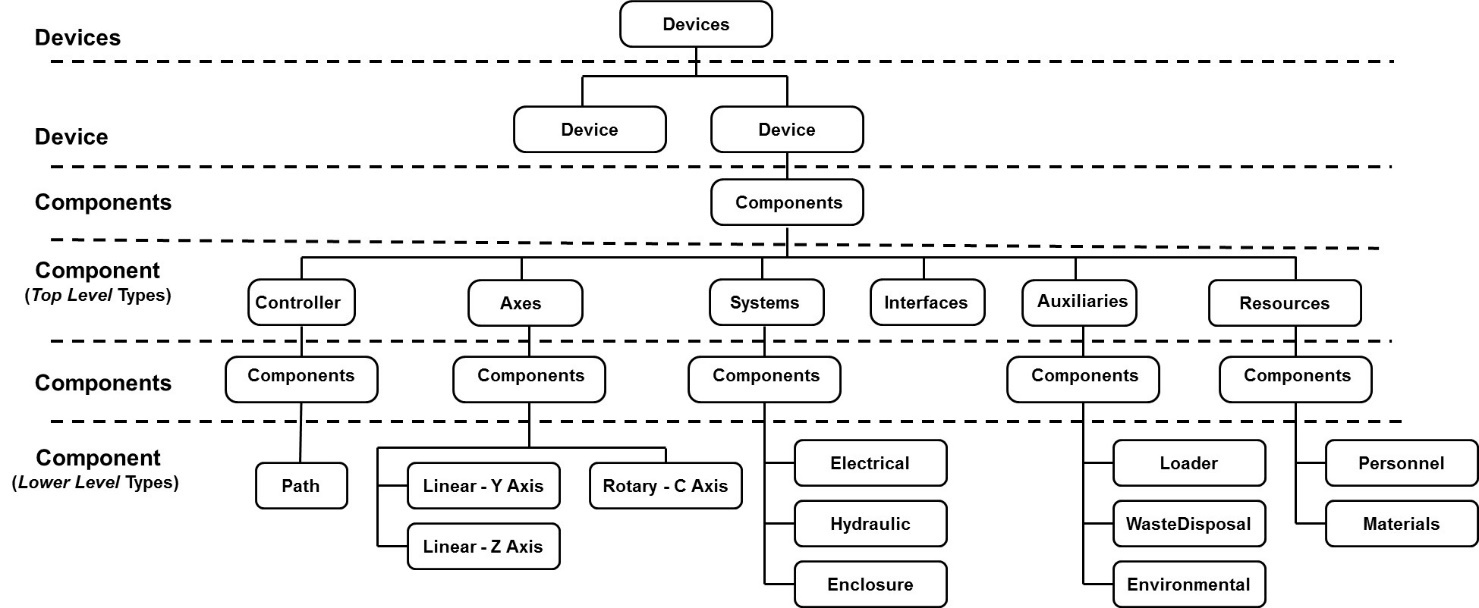
\includegraphics[width=0.95\textwidth]{figures/devices-structural-elements.png}
  \caption{Example Device Structural Elements}
  \label{fig:mtconnect-devices-structural-elements}
\end{figure}

\FloatBarrier

\gls{component} type \gls{xml} elements \may be further decomposed into \gls{composition} type \gls{xml} elements. \gls{composition} elements describe the lowest level basic structural or functional building blocks contained within a \gls{component}. Any number of \gls{composition} elements \may be used. Data provided for a \gls{component} provides more specific meaning when it is associated with one of the \gls{composition} elements of the \gls{component}.  The different \gls{composition} types that \may appear in the \gls{xml} document are defined in \sect{Composition Type Structural Elements}.

The \gls{composition} elements are organized into a \gls{compositions} container.  The \gls{compositions} container \may appear in the \gls{xml} document further describing a \gls{component}. If one or more \gls{composition} element(s) is provided to describe a \gls{component}, a \gls{compositions} container \MUST be defined for the \gls{component}.

\lst{component-levels-with-composition} represents an \gls{xml} document structure that demonstrates the relationship between a parent \gls{component} and its \gls{composition} elements.

\begin{lstlisting}[firstnumber=1,escapechar=|,%
    caption={Component levels with Composition},label={lst:component-levels-with-composition}]
<Devices>
  <Device>
    <Components>
      <Axes>  | {\normalfont\it (Component)} |
        <Components>
          <Linear> | {\normalfont\it (Component)} |
            <Compositions>
              <Composition>
              <Composition>
              <Composition>
\end{lstlisting}

\fig{composition-structural-elements} demonstrates this relationship between a \gls{component} and some of its potential \gls{composition} elements.

\begin{figure}[ht]
  \centering
  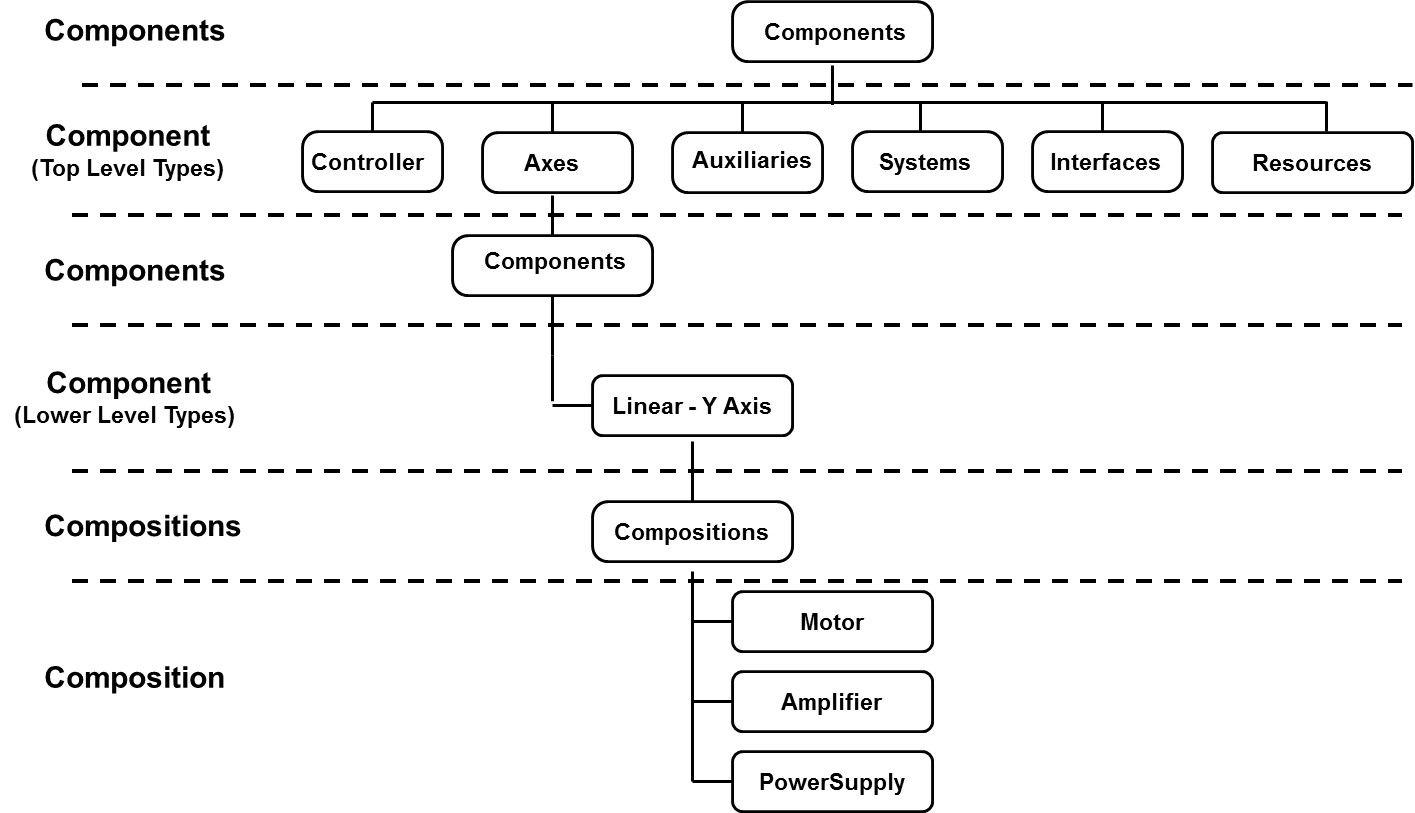
\includegraphics[width=.70\textwidth]{figures/composition-structural-elements.png}
  \caption{Example Composition Structural Elements}
  \label{fig:composition-structural-elements}
\end{figure}

\FloatBarrier

\subsection{Devices}
\label{sec:Devices}

\gls{devices} is a container type \gls{xml} element that \MUST contain only \gls{device} elements. \gls{devices} \MUST contain at least one \gls{device} element, but \may contain multiple \gls{device} elements.  \glspl{data entity} \MAYNOT be directly associated with the \gls{devices} container.

\tabulinesep = 5pt
\begin{longtabu} to \textwidth {
    |l|X[3l]|X[0.75l]|}
\caption{MTConnect Devices Element} \label{table:mtconnect-devices-element} \\

\hline
Element & Description & Occurrence \\
\hline
\endfirsthead

\hline
\multicolumn{3}{|c|}{Continuation of Table \ref{table:mtconnect-devices-element}}\\
\hline
Element & Description & Occurrence \\
\hline
\endhead

\gls{devices}	
&
The first, or highest level, \gls{structural element} in a \gls{mtconnectdevices} document. \gls{devices} is a container type XML element.
&
1 \\
\hline


\end{longtabu}

\pagebreak

\subsection{Device}

\gls{device} is an \gls{xml} container type element that organizes the \glspl{structural element} and \glspl{data entity} associated with a piece of equipment.  \glspl{data entity} \may be directly associated with the \gls{device} container.  \gls{device} \MUST provide the data item \gls{availability event}, which represents the \gls{agent}'s ability to communicate with the data source.

In the \gls{mtconnectdevices} \gls{xml} document, \gls{device} is a unique type of \gls{structural element}.  \gls{device} carries all of the properties of a \gls{component} (See \sect{Component}).  Additionally, \gls{device} \MUST have a \gls{uuid} attribute that uniquely identifies the piece of equipment.  The value for the \gls{uuid} \SHOULDNOT change over time.  The value for the \gls{uuid} \MUST be universally unique and \MUST only appear once in any MTConnect installation.  All \glspl{structural element} and \glspl{data entity} associated with a piece of equipment are therefore uniquely identified through their association with the \gls{device} container.

\tabulinesep = 5pt
\begin{longtabu} to \textwidth {
    |l|X[3l]|X[0.75l]|}
\caption{MTConnect Device Element} \label{table:mtconnect-device-element} \\

\hline
Element & Description & Occurrence \\
\hline
\endfirsthead

\hline
\multicolumn{3}{|c|}{Continuation of Table \ref{table:mtconnect-device-element}}\\
\hline
Element & Description & Occurrence \\
\hline
\endhead

\gls{device}	
&
\glsentrydesc{device} 
There \MAY be multiple \gls{device} elements in an XML document. 
&
1..* \\
\hline


\end{longtabu}


\begin{note}
Note: Some data sources may not be integral to a specific piece of equipment. These data sources may function independently or produce data that is not relevant to a specific piece of equipment. An example would be a temperature sensor installed in a plant to monitor the ambient air temperature. In such a case, these individual data sources, if they singularly or together perform a unique function, \may be modeled in a MTConnect XML document as a \gls{device}. When modeled as a \gls{device}, these data sources \must provide all of the data and capabilities defined for a device.

\end{note}

It is possible for a piece of equipment to be defined as both a \gls{component} of a \gls{device} and simultaneously function independently as a separate \gls{device} reporting data directly through an \gls{agent} using its own \gls{uuid}.  An example would be a temperature monitoring system that is defined as a \gls{device} reporting data about the environment within a facility and simultaneously reporting data for a \gls{component} of another piece of equipment that it is monitoring. 

\subsubsection{XML Schema Structure for Device}

\fig{device-schema-diagram} represents the structure of the \gls{device} XML element showing the attributes defined for \gls{device} and the elements that may be associated with \gls{device}.

\begin{figure}[ht]
  \centering
  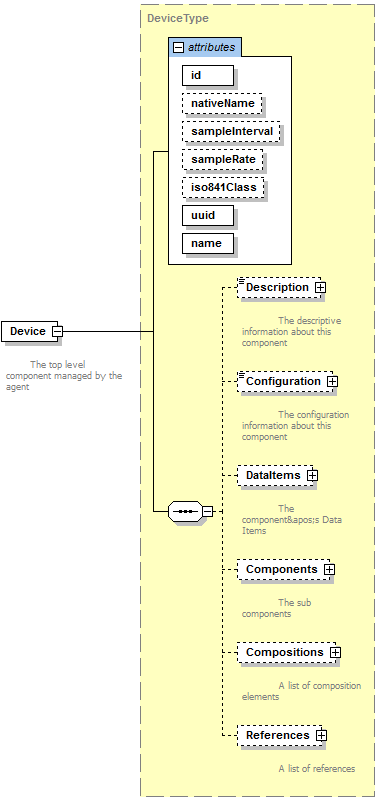
\includegraphics[width=.4\textwidth]{figures/device-schema-diagram.png}
  \caption{Device Diagram}
  \label{fig:device-schema-diagram}
\end{figure}

\FloatBarrier

\subsubsection{Attribute for Device}

\tbl{attributes-for-device} defines the attributes that may be used to provide additional information for a \gls{device} type element.

\tabulinesep = 5pt
\begin{longtabu} to \textwidth {
    |l|X[3l]|X[0.75l]|}
\caption{Attributes for Device} \label{table:attributes-for-device} \\

\hline
Attribute & Description & Occurrence \\
\hline
\endfirsthead

\hline
\multicolumn{3}{|c|}{Continuation of Table \ref{table:attributes-for-device}}\\
\hline
Attribute & Description & Occurrence \\
\hline
\endhead

\gls{id} 
&
\glsentrydesc{id}
\newline \gls{id} is a required attribute.
\newline An \gls{id} \MUST be unique across all the \gls{id} attributes in the document.
\newline An XML ID-type.
&
1 \\
\hline

\gls{nativename}
&
The common name normally associated with this piece of equipment.
\newline \gls{nativename} is an optional attribute. 
&
0..1 \\
\hline

\gls{sampleinterval} 
& 
An optional attribute that is an indication provided by a piece of equipment describing the interval in milliseconds between the completion of the reading of the data associated with the \gls{device} element until the beginning of the next sampling of that data. This indication is reported as the number of milliseconds between data captures.
\newline This information may be used by client software applications to understand how often information from a piece of equipment is expected to be refreshed.
\newline The refresh rate for all data from the piece of equipment will be the same as for the \gls{device} element unless specifically overridden by another \gls{sampleinterval} provided for a \gls{component} of the \gls{device} element.
\newline If the value of \gls{sampleinterval} is less than one millisecond, the value will be represented as a floating-point number. For example, an interval of 100 microseconds would be 0.1.
& 
0..1 \notesign \notesign \\
\hline

\deprecated{\gls{samplerate}}
&
\DEPRECATED in MTConnect Version 1.2. Replaced by \gls{sampleinterval}.
&
0..1 \notesign \notesign \notesign \\
\hline


\deprecated{\gls{iso841class}}
&
\DEPRECATED in MTConnect Version 1.1.
&
0..1 \notesign \notesign \notesign \\
\hline

\gls{uuid}
&
A unique identifier for this XML element.
\newline \gls{uuid} is a required attribute. 
\newline The uuid \MUST be unique amongst all uuid identifiers used in an MTConnect installation. 
\newline For example, this may be a combination of the manufacturer's code and serial number. The \gls{uuid} \SHOULD be alphanumeric and not exceed 255 characters.
\newline An \gls{nmtoken} XML type.
&
1 \notesign \\
\hline

\gls{name}
&
The name of the piece of equipment represented by the \gls{device} element. 
\newline \gls{name} is a required attribute.
\newline This name \MUST be unique for each \gls{device} XML element defined in the \gls{mtconnectdevices} document.
\newline An \gls{nmtoken} XML type.
&
1 \\
\hline

\end{longtabu}


\begin{note}
Notes:
\newline \tab \notesign A \gls{uuid} \MUST be provided for each \gls{device} element.  It is optional for all other \glspl{structural element}.
\newline \tab \notesign \notesign The \gls{sampleinterval} is used to aid a client software application in interpreting values provided by some \glspl{data entity}.  This is the desired sample interval and may vary depending on the capabilities of the piece of equipment.
\newline \tab \notesign \notesign \notesign Remains in schema for backwards compatibility.

\end{note}

\subsubsection{Elements for Device}
\tbl{elements-for-device} lists the elements defined to provide additional information for a \gls{device} element. These elements are organized in the \gls{device} container.

\tabulinesep = 5pt
\begin{longtabu} to \textwidth {
    |l|X[3l]|X[0.75l]|}
\caption{Elements for Device} \label{table:elements-for-device} \\

\hline
Element & Description & Occurrence \\
\hline
\endfirsthead

\hline
\multicolumn{3}{|c|}{Continuation of Table \ref{table:elements-for-device}}\\
\hline
Element & Description & Occurrence \\
\hline
\endhead

\gls{description}
&
An XML element that can contain any descriptive content.
&
0..1 \\
\hline

\gls{configuration}
&
\glsentrydesc{configuration}
&
0..1 \\
\hline

\gls{dataitems}
&
A container for the \glspl{data entity} (See \sect{Data Entities for Device} and \sect{Listing of Data Items} for more detail) provided by this \gls{device} element.
&
1 \notesign \\
\hline

\gls{components}
&
A container for the \gls{component} elements associated with this \gls{device} element.
&
0..1 \\
\hline

\gls{compositions}
&
A container for the \gls{composition} elements associated with this \gls{device} element. 
&
0..1 \\
\hline

\gls{references}
&
A container for the \gls{reference} elements associated with this \gls{device} element.
&
0..1 \\
\hline

\end{longtabu}

\begin{note}
    Note: \notesign \gls{dataitems} \MUST be provided since every piece of equipment \MUST report \gls{availability event}.

\end{note}


\paragraph{Description for Device}\mbox{}

\fig{description-schema-diagram} shows the structure of the \gls{description} XML element showing the attributes defined for \gls{description}.  \gls{description} can contain any descriptive content for this piece of equipment.  This element is defined to contain mixed content and additional XML elements (indicated by the \gls{any} element) \may be added to extend the schema for \gls{description}.

\begin{figure}[ht]
  \centering
  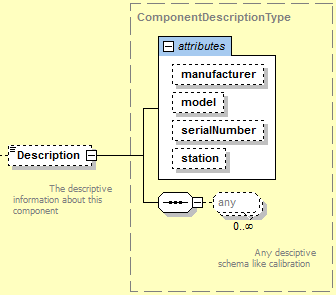
\includegraphics[width=.75\textwidth]{figures/description-schema-diagram.png}
  \caption{Description Diagram}
  \label{fig:description-schema-diagram}
\end{figure}

\FloatBarrier

\tbl{attributes-for-description} lists the attributes defined for the \gls{description} XML element.

\tabulinesep = 5pt
\begin{longtabu} to \textwidth {
    |l|X[3l]|X[0.75l]|}
\caption{Attributes for Description} \label{table:attributes-for-description} \\

\hline
Attribute & Description & Occurrence \\
\hline
\endfirsthead

\hline
\multicolumn{3}{|c|}{Continuation of Table \ref{table:attributes-for-description}}\\
\hline
Attribute & Description & Occurrence \\
\hline
\endhead

\gls{manufacturer}
&
The name of the manufacturer of the piece of equipment represented by the \gls{device} element. 
\newline \gls{manufacturer} is an optional attribute.
&
0..1 \\
\hline

\gls{model}
&
The model description of the piece of equipment represented by the \gls{device} element.
\newline \gls{model} is an optional attribute.
&
0..1 \\
\hline

\gls{serialnumber}
&
The serial number associated with piece of equipment represented by the \gls{device} element. 
\newline \gls{serialnumber} is an optional attribute.
&
0..1 \\
\hline

\gls{station}
&
The station where the equipment represented by the \gls{device} element is located when it is part of a manufacturing unit or cell with multiple stations. 
\newline \gls{station} is an optional attribute.
&
0..1 \\
\hline

\end{longtabu}

The content of \gls{description} \may include any additional descriptive information the implementer chooses to include regarding a piece of equipment.  This content \should be limited to information not included elsewhere in the \gls{mtconnectdevices} XML document.

\begin{lstlisting}[firstnumber=1,escapechar=|,%
    caption={Example of  Description},label={lst:example-of-description}]
<Description manufacturer="Example Co" 
    serialNumber="A124FFF" station="2"> Example Co 
    Simulated Vertical 3 Axis Machining center.
</Description>
\end{lstlisting}

\paragraph{Configuration for Device}\mbox{}
\DIFaddbegin \label{sec:Configuration for Device}
\DIFaddend 

The \gls{configuration} XML element contains technical information about a piece of equipment.  \gls{configuration} \DIFdelbegin \DIFdel{\may }\DIFdelend \DIFaddbegin \DIFadd{\MAY }\DIFaddend include any information describing the physical layout or functional characteristics of the piece of equipment, such as capabilities, testing, installation, operation, calibration, or maintenance. \DIFaddbegin \DIFadd{\gls{configuration} \MAY also include information representing the inter-relationships between pieces of equipment.}\DIFaddend 

\DIFdelbegin \DIFdel{Not all types of equipment support \gls{configuration}.
When \gls{configuration} is supported, details on the schema for \gls{configuration} will be included in the applicable sections. 
}%DIFDELCMD < 

%DIFDELCMD < %%%
\DIFdelend \tabulinesep = 5pt
\begin{longtabu} to \textwidth {
    |l|X[3l]|X[0.75l]|}
\caption{MTConnect Configuration Element} \label{table:mtconnect-configuration-element} \\

\hline
Element & Description & Occurrence \\
\hline
\endfirsthead

\hline
\multicolumn{3}{|c|}{Continuation of Table \ref{table:mtconnect-configuration-element}}\\
\hline
Element & Description & Occurrence \\
\hline
\endhead

\gls{configuration}
&
\DIFdelbegin \DIFdel{\glsentrydesc{configuration}
}\DIFdelend \DIFaddbegin \DIFadd{An XML element that contains technical information about a piece of equipment describing its physical layout, functional characteristics, and relationships with other pieces of equipment.
}\DIFaddend &
0..1 \\
\hline


\end{longtabu}

Configuration data for \gls{device} is structured in the \gls{mtconnectdevices} XML document as shown \DIFdelbegin \DIFdel{in  \fig{configuration-schema-diagram}}\DIFdelend \DIFaddbegin \DIFadd{below}\DIFaddend .   \gls{abstractconfiguration} is an abstract type XML element.   It will never appear in the XML document representing a piece of equipment.    When \gls{configuration} is \DIFdelbegin \DIFdel{supported for a type }\DIFdelend \DIFaddbegin \DIFadd{provided for a piece }\DIFaddend of equipment, that \DIFdelbegin \DIFdel{configuration }\DIFdelend \DIFaddbegin \DIFadd{type of \gls{configuration} }\DIFaddend will appear in the XML document.
\DIFdelbegin \DIFdel{Currently, \gls{sensor} is the only type of equipment that supports \gls{configuration}.  }\DIFdelend \DIFaddbegin 

\DIFaddend \gls{sensorconfiguration} is described in detail in \sect{Sensor Configuration}.

\DIFaddbegin \DIFadd{\gls{relationships} is described in detail in \sect{Relationships}.
}\DIFaddend \begin{figure}[ht]
  \centering
  \DIFdelbeginFL %DIFDELCMD < 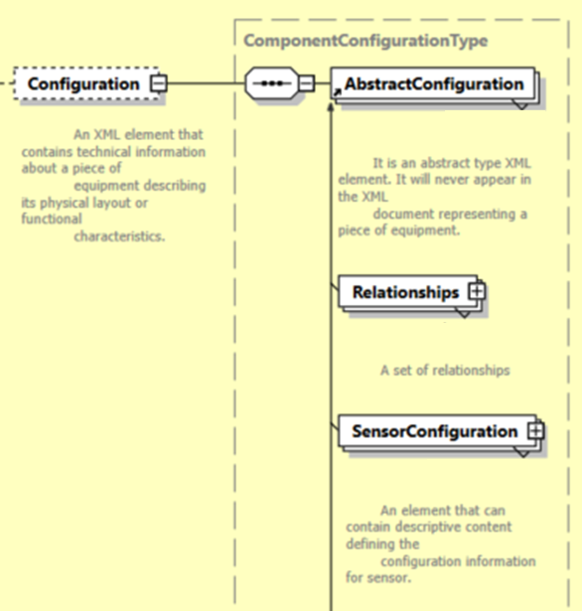
\includegraphics[width=.75\textwidth]{figures/configuration-schema-diagram.png}
%DIFDELCMD <   %%%
\DIFdelendFL \DIFaddbeginFL 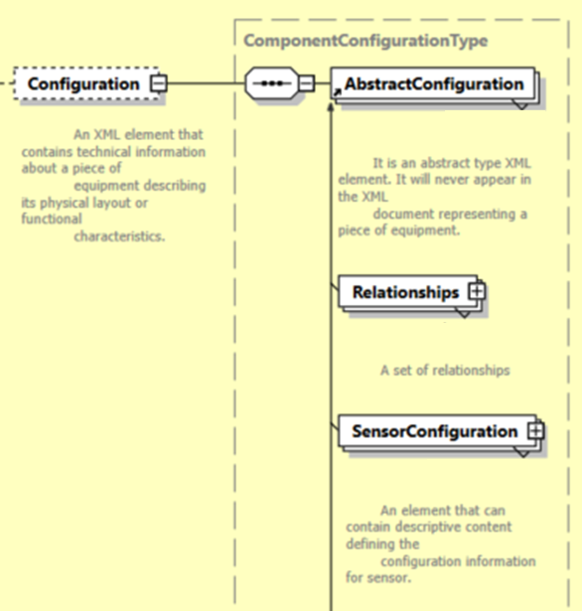
\includegraphics[width=0.7\textwidth]{figures/configuration-schema-diagram.png}
  \DIFaddendFL \caption{Configuration Diagram}
  \label{fig:configuration-schema-diagram}
\end{figure}\FloatBarrier

\DIFdelbegin %DIFDELCMD < \FloatBarrier
%DIFDELCMD < 

%DIFDELCMD < %%%
\DIFdelend \paragraph{DataItems for Device}\mbox{}

\gls{dataitems} is an XML container that provides structure for organizing the data reported by a piece of equipment that is associated with the \gls{device} element.   

\gls{dataitems} \MUST be provided since every piece of equipment \MUST report the data item \gls{availability event}.

See \sect{Data Entities for Device} and \sect{Listing of Data Items} for details on the \gls{dataitems} XML element.

\pagebreak

\paragraph{Components within Device}\mbox{}

The use of the XML container \gls{components} within a \gls{device} element provides the ability to break down the structure of a \gls{device} element into \gls{top level} and \gls{lower level} physical and logical sub-parts.  If a \gls{components} XML element is provided, then only one \gls{components} element \MUST be defined for a \gls{device} element.

\paragraph{Compositions for Device}\mbox{}

\gls{compositions} is an XML container used to organize \gls{composition} elements associated with a \gls{device} element.  See \sect{Compositions} for details on \gls{compositions}.

\paragraph{References for Device}\mbox{}

\gls{references} is an XML container used to organize \gls{references} elements associated with a \gls{device} element.  See \sect{References} for details on \gls{references}.  

\subsection{Components}

\gls{components} is an XML container used to group information describing physical parts or logical functions of a piece of equipment.   \gls{components} contains one or more \gls{component} XML elements.

\tabulinesep = 5pt
\begin{longtabu} to \textwidth {
    |l|X[3l]|X[0.75l]|}
\caption{MTConnect Components Element} \label{table:mtconnect-components-element} \\

\hline
Element & Description & Occurrence \\
\hline
\endfirsthead

\hline
\multicolumn{3}{|c|}{Continuation of Table \ref{table:mtconnect-components-element}}\\
\hline
Element & Description & Occurrence \\
\hline
\endhead

\gls{components}
&
\glsentrydesc{components}
\newline If a \gls{components} XML element is provided, then only one \gls{components} element \MUST be defined for a \gls{device} element.
&
0..1 \\
\hline


\end{longtabu}

\subsection{Component}
\label{sec:Component}

A \gls{component} XML element is a container type XML element used to organize information describing a physical part or logical function of a piece of equipment.   It also provides structure for describing the \gls{lower level} \glspl{structural element} associated with the \gls{component}.     \gls{component} is an abstract type XML element and will never appear directly in the MTConnect XML document.  As an abstract type XML element, \gls{component} will be replaced in the XML document by specific \gls{component} types.  XML elements representing \gls{component} are described in \sect{Component Structural Elements} and include elements such as \gls{axes}, \gls{controller}, and \gls{systems}.

\tabulinesep = 5pt
\begin{longtabu} to \textwidth {
    |l|X[3l]|X[0.75l]|}
\caption{MTConnect Component Element} \label{table:mtconnect-component-element} \\

\hline
Element & Description & Occurrence \\
\hline
\endfirsthead

\hline
\multicolumn{3}{|c|}{Continuation of Table \ref{table:mtconnect-component-element}}\\
\hline
Element & Description & Occurrence \\
\hline
\endhead

\gls{component}
&
\glsentrydesc{component}
\newline There can be multiple types of \gls{component} XML elements in the document.
&
1..* \\
\hline


\end{longtabu}

\subsubsection{XML Schema Structure for Component}
\label{sec:XML Schema Structure for Component}

\fig{component-schema-diagram} represents the structure of a \gls{component} XML element showing the attributes defined for \gls{component} and the elements that \may be associated with \gls{component}.

\begin{figure}[ht]
  \centering
  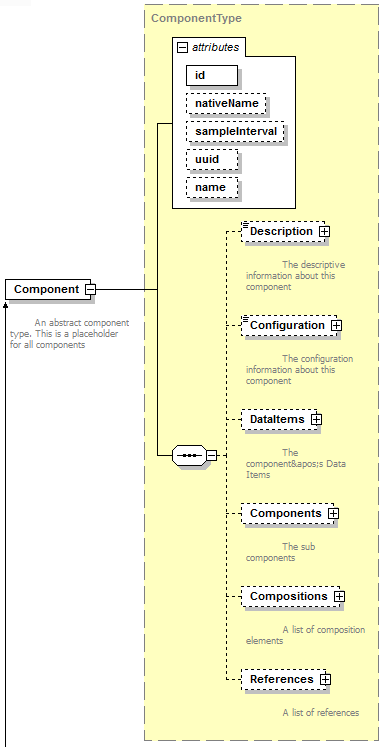
\includegraphics[width=.5\textwidth]{figures/component-schema-diagram.png}
  \caption{Component Diagram}
  \label{fig:component-schema-diagram}
\end{figure}

\FloatBarrier

\subsubsection{Attribute for Component}

\tbl{attributes-for-component} defines the attributes that may be used to provide additional information for a \gls{component} type XML element.

\tabulinesep = 5pt
\begin{longtabu} to \textwidth {
    |l|X[3l]|X[0.75l]|}
\caption{Attributes for  Component} \label{table:attributes-for-component} \\

\hline
Attribute & Description & Occurrence \\
\hline
\endfirsthead

\hline
\multicolumn{3}{|c|}{Continuation of Table \ref{table:attributes-for-component}}\\
\hline
Attribute & Description & Occurrence \\
\hline
\endhead

\gls{id} 
&
\glsentrydesc{id}
\newline \gls{id} is a required attribute.
\newline An \gls{id} \MUST be unique across all the \gls{id} attributes in the document.
\newline An XML ID-type.
&
1 \\
\hline

\gls{nativename}
&
The common name normally associated with a specific physical or logical part of a piece of equipment.
\newline \gls{nativename} is an optional attribute. 
&
0..1 \\
\hline

\gls{sampleinterval}
&
An optional attribute that is an indication provided by a piece of
equipment describing the interval in milliseconds between the
completion of the reading of the data associated with the \gls{component} element until the beginning of the next sampling of that data. This indication is reported as the number of milliseconds between data captures.
\newline This information may be used by client software applications to understand how often information from a piece of equipment for a specific \gls{component} element is expected to be refreshed.
\newline The refresh rate for data from all \gls{lower level} \gls{component} elements will be the same as for the parent \gls{component} element unless specifically overridden by another \gls{sampleinterval} provided for the \gls{lower level} \gls{component} element.
\newline If the value of \gls{sampleinterval} is less than one millisecond, the value will be represented as a floating-point number. For example, an interval of 100 microseconds would be 0.1.
&
0..1 \notesign \notesign \\
\hline


\deprecated{\gls{samplerate}}
&
\DEPRECATED in MTConnect Version 1.2. Replaced by \gls{sampleinterval}.
&
0..1 \notesign \notesign \notesign \\
\hline

\gls{uuid}
&
A unique identifier for this XML element.
\newline \gls{uuid} is an optional attribute. 
\newline The value provided for the \gls{uuid} \MUST be unique amongst all \gls{uuid} identifiers used in an MTConnect installation. 
\newline For example, this may be a combination of the manufacturer's code and serial number. The \gls{uuid} \SHOULD be alphanumeric and not exceed 255 characters.
\newline An \gls{nmtoken} XML type.
&
0..1 \notesign \\
\hline

\gls{name}
&
The name of the \gls{component} element.
\newline \gls{name} is an optional attribute.
\newline However, if there are multiple \gls{lower level} components that have the same parent and are of the same component type (example \gls{linear}), then the name attribute \MUST be provided for all \gls{lower level} components of the same element type to differentiate between the similar components.
\newline When provided, name \MUST be unique for all \gls{lower level} components of a parent \gls{component}.
\newline An \gls{nmtoken} XML type.
&
0..1 \\
\hline

\end{longtabu}

\begin{note}
Notes:

    \tab \notesign While \gls{uuid} \must be provided for the \gls{device} element, it is optional for \gls{component} elements.

    \tab \notesign \notesign The \gls{sampleinterval} is used to aid a client software application in interpreting values provided by some \glspl{data entity}.  This is the desired sample interval and may vary depending on the capabilities of the piece of equipment.

    \tab \notesign \notesign \notesign Remains in schema for backwards compatibility.

\end{note}

\subsubsection{Elements of Component}

\tbl{elements-for-component} lists the elements defined to provide additional information for a \gls{component} type XML element.

\tabulinesep = 5pt
\begin{longtabu} to \textwidth {
    |l|X[3l]|X[0.75l]|}
\caption{Elements for Component} \label{table:elements-for-component} \\

\hline
Element & Description & Occurrence \\
\hline
\endfirsthead

\hline
\multicolumn{3}{|c|}{Continuation of Table \ref{table:elements-for-component}}\\
\hline
Element & Description & Occurrence \\
\hline
\endhead

\gls{description}
&
An element that can contain any descriptive content.
&
0..1 \\
\hline

\gls{configuration}
&
\glsentrydesc{configuration}
&
0..1 \\
\hline

\gls{dataitems}
&
A container for the \glspl{data entity} (defined in \sect{Listing of Data Items}) associated with this \gls{component} element.
&
0..1 \notesign \\
\hline

\gls{components}
&
A container for \gls{lower level} \gls{component} XML elements associated with this parent \gls{component}.
&
0..1 \notesign \\
\hline

\gls{compositions}
&
A container for the \gls{composition} elements (defined in \sect{Composition Type Structural Elements}) associated with this \gls{component} element. 
&
0..1 \\
\hline

\gls{references}
&
A container for the \gls{reference} elements associated with this
\gls{component} element.
&
0..1 \notesign \\
\hline

\end{longtabu}

\begin{note}
    Notes: \notesign At least one of \gls{components}, \gls{dataitems}, or \gls{references} \must be provided.

\end{note}

\paragraph{Description for Component}\mbox{}

\fig{description-of-component-schema-diagram} illustrates the structure of the \gls{description} XML element showing the attributes defined for \gls{description}.  \gls{description} can contain any descriptive content of this \gls{component}.  This element is defined to contain mixed content and additional XML elements (indicated by the \gls{any} element) \may be added to extend the schema for \gls{description}.

\begin{figure}[ht]
  \centering
  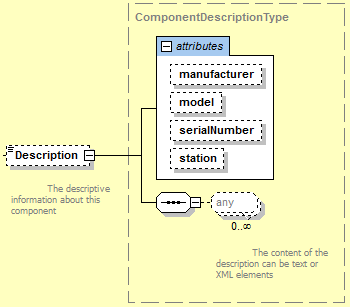
\includegraphics[width=.75\textwidth]{figures/description-of-component-schema-diagram.png}
  \caption{Description of Component Diagram}
  \label{fig:description-of-component-schema-diagram}
\end{figure}

\FloatBarrier

\tbl{attributes-for-component-description} lists the attributes defined for the \gls{description} XML element.

\tabulinesep = 5pt
\begin{longtabu} to \textwidth {
    |l|X[3l]|X[0.75l]|}
\caption{Attributes for Description for Component} \label{table:attributes-for-component-description} \\

\hline
Attribute & Description & Occurrence \\
\hline
\endfirsthead

\hline
\multicolumn{3}{|c|}{Continuation of Table \ref{table:attributes-for-component-description}}\\
\hline
Attribute & Description & Occurrence \\
\hline
\endhead

\gls{manufacturer}
&
The name of the manufacturer of the physical or logical part of a piece of equipment represented by the \gls{component} element. 
\newline \gls{manufacturer} is an optional attribute.
&
0..1 \\
\hline

\gls{model}
&
The model description of the physical part or logical function of a piece of equipment represented by the \gls{component} element.
\newline \gls{model} is an optional attribute.
&
0..1 \\
\hline

\gls{serialnumber}
&
The serial number associated with the physical part or logical function of a piece of equipment represented by the \gls{component} element. 
\newline \gls{serialnumber} is an optional attribute.
&
0..1 \\
\hline

\gls{station}
&
The station where the physical part or logical function of a piece of equipment represented by the \gls{component} element is located when it is part of a manufacturing unit or cell with multiple stations. 
\newline \gls{station} is an optional attribute.
&
0..1 \\
\hline

\end{longtabu}

The content of \gls{description} \may include any additional descriptive information the implementer chooses to include regarding the \gls{component} element. This content \should be limited to information not included elsewhere in the \gls{mtconnectdevices} XML document.  

\begin{lstlisting}[firstnumber=1,escapechar=|,%
    caption={Example of  Description},label={lst:example-of-description-for-component}]
<Description manufacturer="Example Co" 
    serialNumber="EXCO-TT-099PP-XXXX"> Advanced Pulse
    watt-hour transducer with pulse output
</Description>
\end{lstlisting}

\paragraph{Configuration for Component}\DIFdelbegin %DIFDELCMD < \label{sec:Configuration for Component}%%%
\DIFdel{\mbox{}
}\DIFdelend \DIFaddbegin \DIFadd{\mbox{}
}\label{sec:Configuration for Component}
\DIFaddend 

The \gls{configuration} XML element contains technical information about a component.  \gls{configuration} \DIFdelbegin \DIFdel{\may }\DIFdelend \DIFaddbegin \DIFadd{\MAY }\DIFaddend include any information describing the physical layout or functional characteristics of a component, such as capabilities, testing, installation, operation, calibration, or maintenance. \DIFdelbegin %DIFDELCMD < 

%DIFDELCMD < %%%
\DIFdel{Not all \gls{component} types support \gls{configuration} .  When \gls{configuration} is supported, details on the schema for \gls{configuration} will be included in the applicable sections of the MTConnect Standard}\DIFdelend \DIFaddbegin \DIFadd{\gls{configuration} \MAY also include information representing the inter-relationships between components within a piece of equipment}\DIFaddend .

\tabulinesep = 5pt
\begin{longtabu} to \textwidth {
    |l|X[3l]|X[0.75l]|}
\caption{MTConnect Configuration Element for Component} \label{table:mtconnect-configuration-element-for-component} \\

\hline
Element & Description & Occurrence \\
\hline
\endfirsthead

\hline
\multicolumn{3}{|c|}{Continuation of Table \ref{table:mtconnect-configuration-element-for-component}}\\
\hline
Element & Description & Occurrence \\
\hline
\endhead

\gls{configuration}
&
\DIFdelbegin \DIFdel{\glsentrydesc{configuration}
}\DIFdelend \DIFaddbegin \DIFadd{An XML element that contains technical information about a component describing its physical layout, functional characteristics, and relationships with other components within a piece of equipment.
}\DIFaddend &
0..1 \\
\hline


\end{longtabu}

\DIFdelbegin \DIFdel{\gls{configuration} }\DIFdelend \DIFaddbegin \DIFadd{Configuration }\DIFaddend data for \gls{component} is structured in the \gls{mtconnectdevices} XML document as shown \DIFdelbegin \DIFdel{below}\DIFdelend \DIFaddbegin \DIFadd{in \fig{component-configuration-schema-diagram}}\DIFaddend .   \gls{abstractconfiguration} is an abstract type XML element.   It will never appear in the XML document \DIFdelbegin \DIFdel{for a device}\DIFdelend \DIFaddbegin \DIFadd{representing a piece of equipment}\DIFaddend .    When \gls{configuration} is \DIFdelbegin \DIFdel{supported for a \gls{component} type, that configuration }\DIFdelend \DIFaddbegin \DIFadd{provided for a component, that type of \gls{configuration} }\DIFaddend will appear in the XML document.
\DIFdelbegin \DIFdel{Currently, \gls{sensor} is the only component type that supports \gls{configuration}.  }\DIFdelend \DIFaddbegin 

\DIFaddend \gls{sensorconfiguration} is described in detail in \sect{Sensor Configuration}.

\DIFaddbegin \DIFadd{\gls{relationships} is described in detail in \sect{Relationships}.
}\DIFaddend \begin{figure}[ht]
  \centering
  \DIFdelbeginFL %DIFDELCMD < 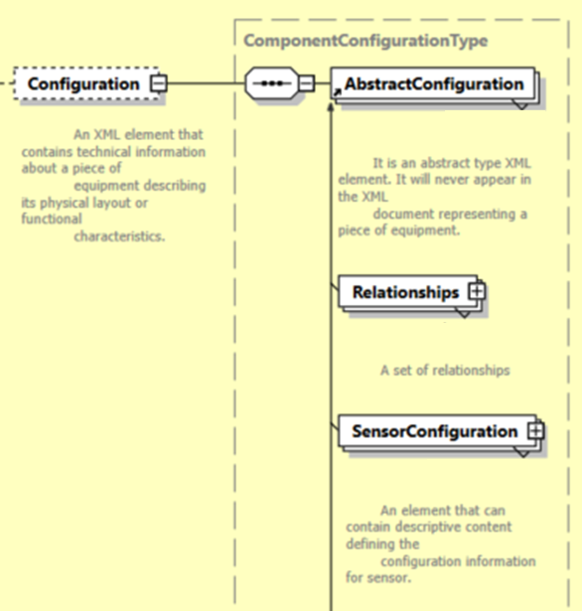
\includegraphics[width=.75\textwidth]{figures/component-configuration-schema-diagram.png}
%DIFDELCMD <   %%%
\DIFdelendFL \DIFaddbeginFL 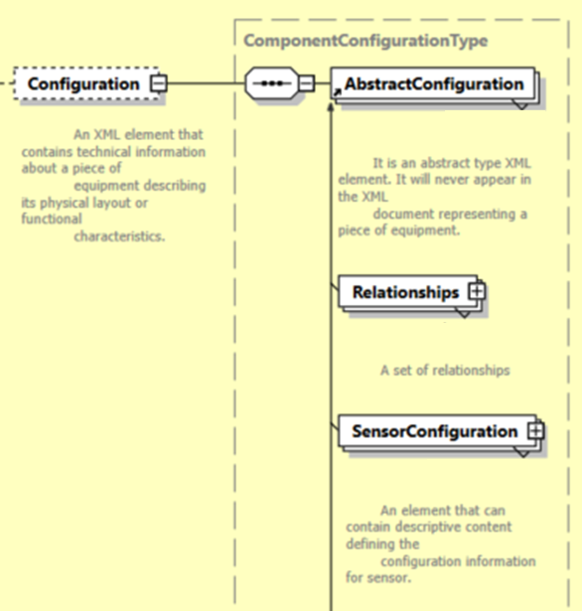
\includegraphics[width=0.7\textwidth]{figures/component-configuration-schema-diagram.png}
  \DIFaddendFL \caption{Component Configuration Diagram}
  \label{fig:component-configuration-schema-diagram}
\end{figure}\FloatBarrier

\DIFdelbegin %DIFDELCMD < \FloatBarrier
%DIFDELCMD < 

%DIFDELCMD < \pagebreak
%DIFDELCMD < 

%DIFDELCMD < %%%
\DIFdelend \paragraph{DataItems for Component}\mbox{}

\gls{dataitems} is an XML container that provides structure for organizing the data reported by a piece of equipment that is associated with the \gls{component}.   

See \sect{Data Entities for Device} for details on the \gls{dataitems} XML element.

\paragraph{Components within Component}\mbox{}

The use of the XML container \gls{components} within a \gls{component} element provides the ability to further break down the structure of a \gls{component} element into even \gls{lower level} physical and logical sub-parts.  These \gls{lower level} elements can add more clarity and granularity to the physical or logical structure of a piece of equipment and the data associated with that equipment.

This parent-child relationship can be extended down to any level necessary to fully describe a piece of equipment. These \gls{lower level} \gls{component} elements use the same XML structure as \gls{component} defined in \sect{XML Schema Structure for Component}.

\begin{lstlisting}[firstnumber=1,escapechar=|,%
    caption={Example of parent Component and Child Elements },label={lst:example-of-parent-component-and-child-elements}]
<Devices>
  <Device>
    <Components>
      <Axes> (Component)
        <Components>
          <Linear> (Component)
            <Components>
              <Etc. > (Component)
\end{lstlisting}

\paragraph{Compositions for Component}\mbox{}

\gls{compositions} is an XML container used to organize the lowest level structural building blocks contained within a \gls{component} as defined below.

\paragraph{References for Component}\mbox{}

\gls{references} is an XML container used to organize \gls{reference} elements associated with a \gls{component} element.  See \sect{References} for details on \gls{references}.

\subsection{Compositions}
\label{sec:Compositions}

\gls{compositions} is an XML container that defines the lowest level structural building blocks contained within a \gls{component} element.   

\gls{compositions} contains one or more \gls{composition} XML elements.

\tabulinesep = 5pt
\begin{longtabu} to \textwidth {
    |l|X[3l]|X[0.75l]|}
\caption{MTConnect Compositions Element} \label{table:mtconnect-compositions-element} \\

\hline
Element & Description & Occurrence \\
\hline
\endfirsthead

\hline
\multicolumn{3}{|c|}{Continuation of Table \ref{table:mtconnect-compositions-element}}\\
\hline
Element & Description & Occurrence \\
\hline
\endhead

\gls{compositions}
&
\glsentrydesc{compositions}
 Only one \gls{compositions} container \MAY appear for a \gls{component} element.
&
0..1 \\
\hline


\end{longtabu}

\subsection{Composition}

\gls{composition} XML elements are used to describe the lowest level physical building blocks of a piece of equipment contained within a \gls{component}.

Like \gls{component} elements, \gls{composition} elements provide the ability to organize information describing \gls{lower level} sub-parts of a higher-level \gls{component} element.  However, unlike \gls{component}, \gls{composition} \mustnot be further sub-divided and \glspl{data entity} \mustnot be assigned to \gls{composition} elements.

\gls{composition} elements are used to add more clarity and granularity to the data being retrieved from a piece of equipment.  The meaning of the data associated with a \gls{component} may be enhanced by designating a specific \gls{composition} element associated with that data.  

An example of the additional detail provided when using \gls{composition} elements would be:

A \gls{temperature sample} associated with a \gls{linear} type axis may be further clarified by referencing the \gls{motor} or \gls{amplifier} type \gls{composition} element associated with that axis, which differentiates the temperature of the motor from the temperature of the amplifier.

\gls{composition} is a typed XML element and will always define a specific type of structural building block contained within a \gls{component}.  XML elements representing the types of \gls{composition} elements are described in \sect{Composition Type Structural Elements} and include elements describing such basic building blocks as motors, amplifiers, filters, and pumps.

\begin{lstlisting}[firstnumber=1,escapechar=|,%
    caption={Example of parent Component and child Composition elements} ,label={lst:example-of-parent-component-and-child-composition-elements}]
<Devices>
  <Device>
    <Components>
      <Axes> (Component)
        <Components>
          <Linear> (Component)
            <Compositions>
              <Composition>
              <Composition>
              <Composition>
\end{lstlisting}

\tabulinesep = 5pt
\begin{longtabu} to \textwidth {
    |l|X[3l]|X[0.75l]|}
\caption{MTConnect Composition Element} \label{table:mtconnect-composition-element} \\

\hline
Element & Description & Occurrence \\
\hline
\endfirsthead

\hline
\multicolumn{3}{|c|}{Continuation of Table \ref{table:mtconnect-composition-element}}\\
\hline
Element & Description & Occurrence \\
\hline
\endhead

\gls{composition}
&
\glsentrydesc{composition}
\newline \gls{composition} is a typed XML element.
\newline There can be multiple types of \gls{composition} XML elements defined for a \gls{component} element.
&
1..* \\
\hline


\end{longtabu}

\subsubsection{XML Schema Structure for Composition}

\fig{composition-schema-diagram} illustrates a \gls{composition} XML element showing the attributes defined for \gls{composition} and the elements that may be associated with \gls{composition} type XML elements.

\begin{figure}[ht]
  \centering
  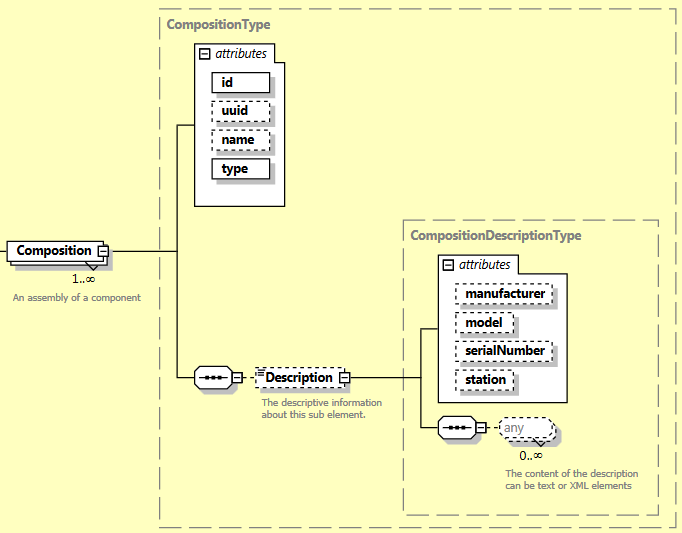
\includegraphics[width=.75\textwidth]{figures/composition-schema-diagram.png}
  \caption{Composition Diagram}
  \label{fig:composition-schema-diagram}
\end{figure}

\FloatBarrier

\subsubsection{Attributes for Composition}

\tbl{attributes-for-composition} defines the attributes that may be used to provide additional information for a \gls{composition} type XML element.

\tabulinesep = 5pt
\begin{longtabu} to \textwidth {
    |l|X[3l]|X[0.75l]|}
\caption{Attributes for Composition} \label{table:attributes-for-composition} \\

\hline
Attribute & Description & Occurrence \\
\hline
\endfirsthead

\hline
\multicolumn{3}{|c|}{Continuation of Table \ref{table:attributes-for-composition}}\\
\hline
Attribute & Description & Occurrence \\
\hline
\endhead

\gls{id} 
&
\glsentrydesc{id}
\newline \gls{id} is a required attribute.
\newline An \gls{id} \MUST be unique across all the \gls{id} attributes in the document.
\newline An XML ID-type.
&
1 \\
\hline

\gls{uuid}
&
A unique identifier for this XML element.
\newline \gls{uuid} is an optional attribute. 
\newline The \gls{uuid} \MUST be unique amongst all \gls{uuid} identifiers used in an MTConnect installation. 
\newline For example, this may be a combination of the manufacturer's code and serial number. The \gls{uuid} \SHOULD be alphanumeric and not exceed 255 characters.
\newline An \gls{nmtoken} XML type.
&
0..1 \\
\hline

\gls{name}
&
The name of the \gls{composition} element.
\newline \gls{name} is an optional attribute.
\newline If provided, \gls{name} \MUST be unique within a \gls{component} element.
\newline An \gls{nmtoken} XML type.
&
0..1 \\
\hline

\gls{type}
&
The type of \gls{composition} element.
\newline \gls{type} is a required attribute.
\newline Examples of types are \gls{motor}, \gls{filter type}, \gls{pump}, and \gls{amplifier}.
\newline Refer to \sect{Composition Type Structural Elements} for a list of currently defined types.
&
1 \\
\hline

\end{longtabu}

\subsubsection{Elements of Composition}

\tbl{elements-for-composition} lists the elements defined to provide additional information for a \gls{composition} type XML element.

\tabulinesep = 5pt
\begin{longtabu} to \textwidth {
    |l|X[3l]|X[0.75l]|}
\caption{Elements for Composition} \label{table:elements-for-composition} \\

\hline
Element & Description & Occurrence \\
\hline
\endfirsthead

\hline
\multicolumn{3}{|c|}{Continuation of Table \ref{table:elements-for-composition}}\\
\hline
Element & Description & Occurrence \\
\hline
\endhead

\gls{description}
&
An element that can contain any descriptive content.
&
0..1 \\
\hline

\end{longtabu}

\paragraph{Description for Composition}\mbox{}

\fig{description-of-composition-schema-diagram} represents the structure of the \gls{description} XML element showing the attributes defined for \gls{description}.  \gls{description} can contain any descriptive content for this \gls{composition} element.  This element is defined to contain mixed content and additional XML elements (indicated by the \gls{any} element) \may be added to extend the schema for \gls{description}.

\begin{figure}[ht]
  \centering
  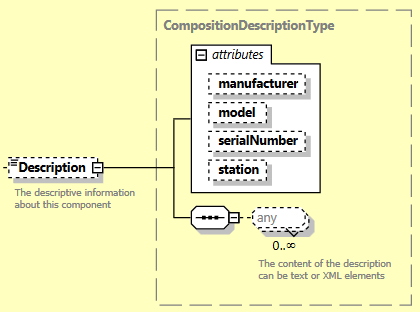
\includegraphics[width=.75\textwidth]{figures/description-of-composition-schema-diagram.png}
  \caption{Description of Composition Diagram}
  \label{fig:description-of-composition-schema-diagram}
\end{figure}

\FloatBarrier

\newpage

\tbl{attributes-for-composition-description} lists the attributes defined for the \gls{description} XML element. 

\tabulinesep = 5pt
\begin{longtabu} to \textwidth {
    |l|X[3l]|X[0.75l]|}
\caption{Attributes for Description for Composition} \label{table:attributes-for-composition-description} \\

\hline
Attribute & Description & Occurrence \\
\hline
\endfirsthead

\hline
\multicolumn{3}{|c|}{Continuation of Table \ref{table:attributes-for-composition-description}}\\
\hline
Attribute & Description & Occurrence \\
\hline
\endhead

\gls{manufacturer}
&
The name of the manufacturer of the physical part of a piece of equipment represented by the \gls{composition} element. 
\newline \gls{manufacturer} is an optional attribute.
&
0..1 \\
\hline

\gls{model}
&
The model description of the physical part of a piece of equipment represented by the \gls{composition} element.
\newline \gls{model} is an optional attribute.
&
0..1 \\
\hline

\gls{serialnumber}
&
The serial number associated with the physical part of a piece of equipment represented by the \gls{composition} element. 
\newline \gls{serialnumber} is an optional attribute.
&
0..1 \\
\hline

\gls{station}
&
The station where the physical part of a piece of equipment represented by the \gls{composition} element is located when it is part of a manufacturing unit or cell with multiple stations. 
\newline \gls{station} is an optional attribute.
&
0..1 \\
\hline

\end{longtabu}

The content of \gls{description} \may include any additional descriptive information the implementer chooses to include regarding the \gls{composition} element.  This content \should be limited to information not included elsewhere in the \gls{mtconnectdevices} XML document.

\begin{lstlisting}[firstnumber=1,escapechar=|,%
    caption={Example of  Description},label={lst:example-of-description-for-composition}]
<Description manufacturer="Example Co" 
    serialNumber="A124FFF" station="2"> Spindle motor
    associated with Path 2.
</Description>
\end{lstlisting}

\subsection{References}
\label{sec:References}

\gls{references} is an XML container that organizes pointers to information defined elsewhere within the XML document for a piece of equipment.

\gls{references} may be modeled as part of a \gls{device}, \gls{component} or \gls{interface component} type \gls{structural element}.

\gls{references} contains one or more \gls{reference} XML elements.

\tabulinesep = 5pt
\begin{longtabu} to \textwidth {
    |l|X[3l]|X[0.75l]|}
\caption{MTConnect References Element} \label{table:mtconnect-references-element} \\

\hline
Element & Description & Occurrence \\
\hline
\endfirsthead

\hline
\multicolumn{3}{|c|}{Continuation of Table \ref{table:mtconnect-references-element}}\\
\hline
Element & Description & Occurrence \\
\hline
\endhead

\gls{references}	
&
\glsentrydesc{references}
 Only one \gls{references} container \MUST appear for a \gls{device}, \gls{component}, or \gls{interface} element.
&
0..1 \\
\hline


\end{longtabu}

\subsection{Reference}

\gls{reference} is a pointer to information that is associated with another \gls{structural element} defined elsewhere in the XML document for a piece of equipment.  That information may be data from the other element or the entire structure of that element.

\gls{reference} is an efficient method to associate information with an element without duplicating any of the data or structure.  For example, a Bar Feeder System may make a request for the \gls{barfeederinterface} and receive all the relevant data for the interface and the associated spindle (\gls{rotary} element) that is referenced as part of the \gls{barfeederinterface}.

\gls{reference} is an abstract type XML element and will never appear directly in the MTConnect XML document.  As an abstract type XML element, \gls{reference} will be replaced in the XML document by a specific \gls{reference} type.  The current supported types of \gls{reference} are \gls{dataitemref} and \gls{componentref} XML elements.

\fig{reference-schema-diagram} represents the structure of the \gls{reference} XML element.

\begin{figure}[ht]
  \centering
  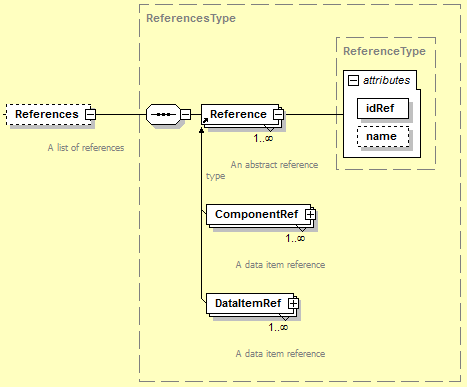
\includegraphics[width=.75\textwidth]{figures/reference-schema-diagram.png}
  \caption{Reference Diagram}
  \label{fig:reference-schema-diagram}
\end{figure}
\FloatBarrier

\subsubsection{ComponentRef}

\gls{componentref} XML element is a pointer to all of the information associated with another \gls{structural element} defined elsewhere in the XML document for a piece of equipment.  \gls{componentref} allows all of the information (\gls{lower level} \gls{components} and all \glspl{data entity}) that is associated with the other \gls{structural element} to be directly associated with this XML element.

\fig{componentref-schema-diagram} represents the structure of a \gls{componentref} XML element showing the attributes defined for \gls{componentref}.

\begin{figure}[ht]
  \centering
  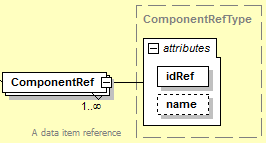
\includegraphics[width=.5\textwidth]{figures/componentref-schema-diagram.png}
  \caption{ComponentRef Diagram}
  \label{fig:componentref-schema-diagram}
\end{figure}

\FloatBarrier

\tbl{attributes-for-componentref} lists the attributes defined for the \gls{componentref} element. 

\tabulinesep = 5pt
\begin{longtabu} to \textwidth {
    |l|X[3l]|X[0.75l]|}
\caption{Attributes for ComponentRef} \label{table:attributes-for-componentref} \\

\hline
Attribute & Description & Occurrence \\
\hline
\endfirsthead

\hline
\multicolumn{3}{|c|}{Continuation of Table \ref{table:attributes-for-componentref}}\\
\hline
Attribute & Description & Occurrence \\
\hline
\endhead

\gls{idref} 
&
A pointer to the \gls{id} attribute of the \gls{component} that contains the information to be associated with this XML element.
\newline \gls{idref} is a required attribute.
&
1 \\
\hline

\gls{name}
&
The name of the \gls{componentref} element.
\newline \gls{name} is an optional attribute.
\newline However, if there are multiple \gls{componentref} elements defined for a \gls{component}, the \gls{name} attribute \MUST be provided for all \gls{componentref} elements to differentiate between the similar elements.
\newline When provided, \gls{name} \MUST be unique for all \gls{componentref} elements associated with the \gls{parent element}.
\newline An \gls{nmtoken} XML type.
&
0..1 \\
\hline

\end{longtabu}

\subsubsection{DataItemRef}

\gls{dataitemref} XML element is a pointer to a \gls{data entity} associated with another \gls{structural element} defined elsewhere in the XML document for a piece of equipment.  \gls{dataitemref} allows the data associated with a data item defined in another \gls{structural element} to be directly associated with this XML element.

\fig{dataitemref-schema-diagram} represents the structure of a \gls{dataitemref} XML element showing the attributes defined for \gls{dataitemref}.

\begin{figure}[ht]
  \centering
  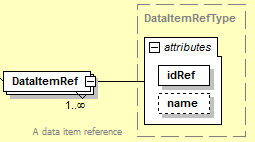
\includegraphics[width=.75\textwidth]{figures/dataitemref-schema-diagram.png}
  \caption{DataItemRef Diagram}
  \label{fig:dataitemref-schema-diagram}
\end{figure}

\FloatBarrier

\tbl{attributes-for-dataitemref} lists the attributes defined for the \gls{dataitemref} element. 

\tabulinesep = 5pt
\begin{longtabu} to \textwidth {
    |l|X[3l]|X[0.75l]|}
\caption{Attributes for DataItemRef} \label{table:attributes-for-dataitemref} \\

\hline
Attribute & Description & Occurrence \\
\hline
\endfirsthead

\hline
\multicolumn{3}{|c|}{Continuation of Table \ref{table:attributes-for-dataitemref}}\\
\hline
Attribute & Description & Occurrence \\
\hline
\endhead

\gls{idref} 
&
A pointer to the \gls{id} attribute of the \gls{dataitem} that contains the information to be associated with this XML element.
\newline \gls{idref} is a required attribute.
&
1 \\
\hline

\gls{name}
&
The name of the \gls{dataitemref} element.
\newline \gls{name} is an optional attribute.
\newline However, if there are multiple \gls{dataitemref} elements defined for a \gls{component}, the \gls{name} attribute \MUST be provided for all \gls{dataitemref} elements to differentiate between the similar elements.
\newline When provided, \gls{name} \MUST be unique for all \gls{dataitemref} elements associated with the \gls{parent element}.
\newline An \gls{nmtoken} XML type.
&
0..1 \\
\hline

\end{longtabu}

\pagebreak

\DIFaddbegin \subsection{\DIFadd{Relationships}}
\label{sec:Relationships}

\DIFadd{\gls{relationships} is an XML container that organizes information defining the association between pieces of equipment that function independently but together perform a manufacturing operation.  \gls{relationships} may also define the association between components within a piece of equipment.
 }

\DIFadd{\gls{relationships} may be modeled as part of a \gls{device} or a \gls{component} \gls{structural element}.
 }

\DIFadd{\gls{relationships} contains one or more \gls{relationship} XML elements.
}


\begin{longtabu} to \textwidth{|l|X[3l]|l|}
\caption{\DIFadd{MTConnect Relationships Element}} \label{table:mtconnect-relationships-element} \\

\hline
\DIFadd{Element }& \DIFadd{Description }& \DIFadd{Occurrence }\\
\hline
\endfirsthead

\hline
\multicolumn{3}{|c|}{Continuation of Table \ref{table:mtconnect-relationships-element}}\\
\hline
\DIFadd{Element }& \DIFadd{Description }& \DIFadd{Occurrence }\\
\hline
\endhead





\DIFadd{\gls{relationships}
}&
\DIFadd{XML container consisting of one or more \gls{relationship} XML elements.
}\newline \DIFadd{Only one \gls{relationships} container \MUST appear for a \gls{device} or a \gls{component} element.
}&
\DIFadd{0..1 }\\
\hline\end{longtabu}


\subsection{\DIFadd{Relationship}}
\label{sec:Relationship}

\DIFadd{\gls{relationship} is an XML element that describes the association between two pieces of equipment that function independently but together perform a manufacturing operation. \gls{relationship} may also be used to define the association between two components within a piece of equipment.
}

\DIFadd{\gls{relationship} is an abstract type XML element, \gls{relationship} will be replaced in the XML document by specific \gls{relationship} types.  XML elements representing \gls{relationship} are described in \sect{DeviceRelationship} and \sect{ComponentRelationship}.
}

\DIFadd{A separate \gls{relationship} type element \MAY be defined to describe each pair of associations with a piece of equipment or between \gls{component} elements within a piece of equipment.}

\DIFadd{Pieces of equipment may only be associated with other pieces of equipment and \gls{component} elements may only be associated with other \gls{component} elements within a specific piece of equipment.}

\DIFadd{The XML schema diagram in \fig{relationship-schema-diagram} represents the structure of the \gls{relationship} XML element.
}

\begin{figure}[ht]
  \centering
  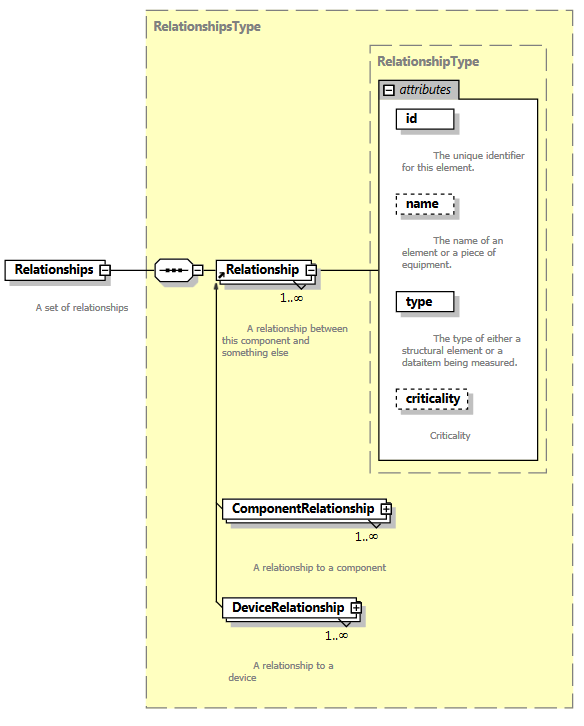
\includegraphics[width=0.75\textwidth]{figures/relationship-schema-diagram.png}
  \caption{\DIFaddFL{Relationship Diagram}}
  \label{fig:relationship-schema-diagram}
\end{figure}
\FloatBarrier

\subsubsection{\DIFadd{DeviceRelationship}}
\label{sec:DeviceRelationship}

\DIFadd{\gls{devicerelationship} describes the association between two pieces of equipment that function independently but together perform a manufacturing operation.
}

\DIFadd{The XML schema diagram in \fig{devicerelationship-schema-diagram} represents the structure of a \gls{devicerelationship} XML element showing the attributes defined for \gls{devicerelationship}.
}\begin{figure}[ht]
  \centering
  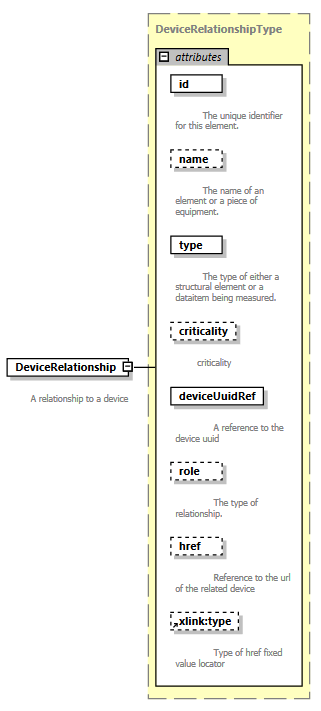
\includegraphics[width=0.6\textwidth]{figures/devicerelationship-schema-diagram.png}
  \caption{\DIFaddFL{DeviceRelationship Diagram}}
  \label{fig:devicerelationship-schema-diagram}
\end{figure}
\FloatBarrier

\DIFadd{The \tbl{attributes-for-devicerelationship} lists the attributes defined for the \gls{devicerelationship} element.
}


\begin{longtabu} to \textwidth{|l|X[3l]|l|}
\caption{\DIFadd{Attributes for DeviceRelationship}} \label{table:attributes-for-devicerelationship} \\

\hline
\DIFadd{Attribute }& \DIFadd{Description }& \DIFadd{Occurrence }\\
\hline
\endfirsthead

\hline
\multicolumn{3}{|c|}{Continuation of Table \ref{table:attributes-for-devicerelationship}}\\
\hline
\DIFadd{Attribute }& \DIFadd{Description }& \DIFadd{Occurrence }\\
\hline
\endhead





\DIFadd{\gls{id}
}&
\DIFadd{The unique identifier for this \gls{devicerelationship}.
}\newline \DIFadd{\gls{id} is a required attribute.
}\newline \DIFadd{The \gls{id} attribute \MUST be unique within the \gls{mtconnectdevices} document.
}\newline \DIFadd{An XML ID-type.
}&
\DIFadd{1 }\\
\hline

\DIFadd{\gls{name}
}&
\DIFadd{The name associated with this \gls{devicerelationship}.
}\newline \DIFadd{\gls{name} is provided as an additional human readable identifier for this \gls{devicerelationship}.
}\newline \DIFadd{\gls{name} is an optional attribute.
}\newline \DIFadd{An NMTOKEN XML type.
}&
\DIFadd{0..1 }\\
\hline

\DIFadd{\gls{type}
}&
\DIFadd{Defines the authority that this piece of equipment has relative to the associated piece of equipment.
}\newline \DIFadd{\gls{type} is a required attribute.
}\newline \DIFadd{The value provided for \gls{type} \MUST be one of the following values:
}\newline 	\DIFadd{\tab \gls{parent}:  This piece of equipment functions as a parent in the relationship with the associated piece of equipment.
}\newline  	\DIFadd{\tab \gls{child}:  This piece of equipment functions as a child in the relationship with the associated piece of equipment.
}\newline  	\DIFadd{\tab \gls{peer}:  This piece of equipment functions as a peer which provides equal functionality and capabilities in the relationship with the associated piece of equipment.
}&
\DIFadd{1 }\\
\hline

\DIFadd{\gls{criticality}
}&
\DIFadd{Defines whether the services or functions provided by the associated piece of equipment is required for the operation of this piece of equipment.
}\newline \DIFadd{\gls{criticality} is an optional attribute.
}\newline \DIFadd{The value provided for \gls{criticality} \MUST be one of the following values:
}\newline 	\DIFadd{\tab \gls{critical}:  The services or functions provided by the associated piece of equipment is required for the operation of this piece of equipment.
}\newline  	\DIFadd{\tab \gls{noncritical}:  The services or functions provided by the associated piece of equipment is not required for the operation of this piece of equipment.
}&
\DIFadd{0..1 }\\
\hline

\DIFadd{\gls{deviceuuidref}
}&
\DIFadd{A reference to the associated piece of equipment.
}\newline \DIFadd{The value provided for \gls{deviceuuidref} \MUST be the value provided for the \gls{uuid} attribute of the \gls{device} element of the associated piece of equipment.
}\newline \DIFadd{\gls{deviceuuidref} is a required attribute.
}\newline \DIFadd{An NMTOKEN XML type.
}&
\DIFadd{1 }\\
\hline

\DIFadd{\gls{role}
}&
\DIFadd{Defines the services or capabilities that the referenced piece of equipment provides relative to this piece of equipment.
}\newline \DIFadd{\gls{role} is an optional attribute.
}\newline \DIFadd{The value provided for \gls{role} \MUST be one of the following values:
}\newline  	\DIFadd{\tab \gls{system condition}:  The associated piece of equipment performs the functions of a \cfont{System} for this piece of equipment.  In MTConnect, \cfont{System} provides utility type services to support the operation of a piece of equipment and these services are required for the operation of a piece of equipment.
}\newline  	\DIFadd{\tab \gls{auxiliary subtype}:  The associated piece of equipment performs the functions as an \cfont{Auxiliary} for this piece of equipment.  In MTConnect, \cfont{Auxiliary} extends the capabilities of a piece of equipment, but is not required for the equipment to function.
}&
\DIFadd{0..1 }\\
\hline

\DIFadd{\gls{href}
}&
\DIFadd{A URI identifying the \gls{agent} that is publishing information for the associated piece of equipment. \gls{href} \MUST also include the UUID for that specific piece of equipment.
}
\newline \DIFadd{\gls{href} is of type \cfont{xlink:href} from the W3C XLink specification: (https://www.w3.org/TR/xlink11/).}
\newline \DIFadd{\gls{href} is an optional attribute.
}&
\DIFadd{0..1 }\\
\hline

\DIFadd{\gls{xlink:type}
}&
\DIFadd{The XLink \cfont{type} attribute \MUST have a fixed value of \cfont{locator} as defined in W3C XLink 1.1 https://www.w3.org/TR/xlink11/ \textit{section 5.4 Locator Attribute (\gls{href})}.}
\newline \DIFadd{If the \gls{href} attribute is provided, it \MUST conform to the URI syntactic rules as defined in IETF RFC 3986 for Uniform Resource Identifiers. (https://www.ietf.org/rfc/rfc3986.txt)}&
\DIFadd{0..1 }\\\hline\end{longtabu}



\subsubsection{\DIFadd{ComponentRelationship}}
\label{sec:ComponentRelationship}

\DIFadd{\gls{componentrelationship} describes the association between two components within a piece of equipment that function independently but together perform a capability or service within a piece of equipment.
}

\DIFadd{The XML schema in \fig{componentrelationship-schema-diagram} represents the structure of a \gls{componentrelationship} XML element showing the attributes defined for \gls{componentrelationship}.
}\begin{figure}[ht]
  \centering
  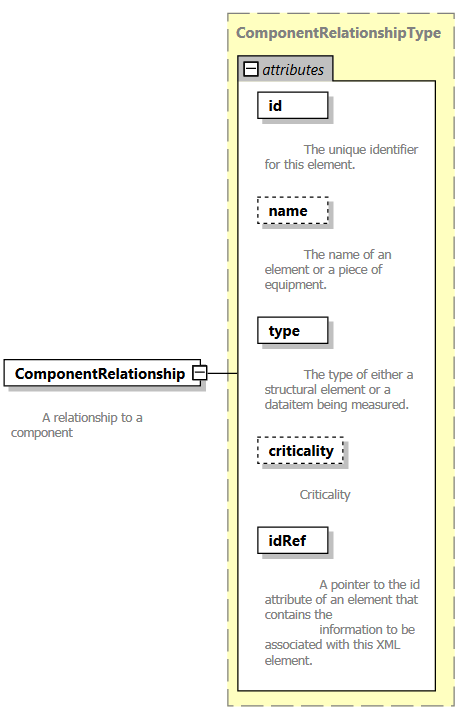
\includegraphics[width=0.75\textwidth]{figures/componentrelationship-schema-diagram.png}
  \caption{\DIFaddFL{ComponentRelationship Diagram}}
  \label{fig:componentrelationship-schema-diagram}
\end{figure}
\FloatBarrier

\DIFadd{The \tbl{attributes-for-componentrelationship} lists the attributes defined for the \gls{componentrelationship} element.
}


\begin{longtabu} to \textwidth{|l|X[3l]|l|}
\caption{\DIFadd{Attributes for ComponentRelationship}} \label{table:attributes-for-componentrelationship} \\

\hline
\DIFadd{Attribute }& \DIFadd{Description }& \DIFadd{Occurrence }\\
\hline
\endfirsthead

\hline
\multicolumn{3}{|c|}{Continuation of Table \ref{table:attributes-for-componentrelationship}}\\
\hline
\DIFadd{Attribute }& \DIFadd{Description }& \DIFadd{Occurrence }\\
\hline
\endhead





\DIFadd{\gls{id}
}&
\DIFadd{The unique identifier for this \gls{componentrelationship}.
}\newline \DIFadd{\gls{id} is a required attribute.
}\newline \DIFadd{The \gls{id} attribute \MUST be unique within the \gls{mtconnectdevices} document.
}\newline \DIFadd{An XML ID-type.
}&
\DIFadd{1 }\\
\hline

\DIFadd{\gls{name}
}&
\DIFadd{The name associated with this \gls{componentrelationship}.
}\newline \DIFadd{\gls{name} is provided as an additional human readable identifier for this \gls{componentrelationship}.
}\newline \DIFadd{\gls{name} is an optional attribute.
}\newline \DIFadd{An NMTOKEN XML type.
}&
\DIFadd{0..1 }\\
\hline

\DIFadd{\gls{type}
}&
\DIFadd{Defines the authority that this component element has relative to the associated component element.
}\newline \DIFadd{\gls{type} is a required attribute.
}\newline \DIFadd{The value provided for \gls{type} \MUST be one of the following values:
}\newline 	\DIFadd{\tab \gls{parent}:  This component functions as a parent in the relationship with the associated component element.
}\newline  	\DIFadd{\tab \gls{child}:  This component functions as a child in the relationship with the associated component element.
}\newline  	\DIFadd{\tab \gls{peer}:  This component functions as a peer which provides equal functionality and capabilities in the relationship with the associated component element.
}&
\DIFadd{1 }\\
\hline

\DIFadd{\gls{criticality}
}&
\DIFadd{Defines whether the services or functions provided by the associated component element is required for the operation of this piece of equipment.
}\newline \DIFadd{\gls{criticality} is an optional attribute.
}\newline \DIFadd{The value provided for \gls{criticality} \MUST be one of the following values:
}\newline 	\DIFadd{\tab \gls{critical}:  The services or functions provided by the associated component element is required for the operation of this piece of equipment.
}\newline  	\DIFadd{\tab \gls{noncritical}:  The services or functions provided by the associated component element is not required for the operation of this piece of equipment.
}&
\DIFadd{0..1 }\\
\hline

\DIFadd{\gls{idref}
}&
\DIFadd{A reference to the associated component element.
}\newline \DIFadd{The value provided for \gls{idref} \MUST be the value provided for the \gls{id} attribute of the associated \gls{component} element.
}\newline \DIFadd{\gls{idref} is a required attribute.
}\newline \DIFadd{An NMTOKEN XML type.
}&
\DIFadd{1 }\\
\hline\end{longtabu}

\DIFaddend \section{Component Structural Elements}
\label{sec:Component Structural Elements}

\gls{component} \glspl{structural element} are XML containers used to represent physical parts or logical functions of a piece of equipment.

\gls{component} \glspl{structural element} are defined into two major categories:

\begin{itemize}

\item \gls{top level} \gls{component} elements are used to group the \glspl{structural element} representing the most significant physical or logical functions of a piece of equipment.  The \gls{top level} \gls{component} elements provided in an \gls{mtconnectdevices} document \should be restricted to those defined in \tbl{elements-toplevel-for-component}.  However, these \gls{top level} \gls{component} elements \may also be used as \gls{lower level} \gls{component} elements; as required.

\item \gls{lower level} \gls{component} elements are used to describe the sub-parts of the parent \gls{component} to provide more clarity and granularity to the physical or logical structure of the \gls{top level} \gls{component} elements.
\end{itemize}

This section of the \glspl{device information model} provides guidance for the most common relationships between \gls{top level} \gls{component} elements and \gls{lower level} child components.  However, all \gls{component} elements \may be used in any configuration, as required, to fully describe a piece of equipment.

As described in \sect{Structural Elements for MTConnectDevices}, \gls{component} is an abstract type \gls{structural element} within the \glspl{device information model} and will never appear directly in the \gls{mtconnectdevices} XML document.  As abstract type XML elements, \gls{component} will be replaced in the XML document by a specific \gls{component} type.

\tbl{elements-toplevel-for-component} defines the \gls{top level} \gls{component} elements available to describe a piece of equipment.

\tabulinesep = 5pt
\begin{longtabu} to \textwidth {
    |l|X[3l]|}
\caption{Top Level Component Elements} \label{table:elements-toplevel-for-component} \\

\hline
Top Level Component Element \notesign \notesign & Description\\
\hline
\endfirsthead

\hline
\multicolumn{2}{|c|}{Continuation of Table \ref{table:elements-toplevel-for-component}}\\
\hline
Top Level Component Element \notesign \notesign & Description\\
\hline
\endhead

\gls{axes}	
&
\glsentrydesc{axes} \\
\hline

\gls{controller}
&
\glsentrydesc{controller}
\\
\hline

\gls{systems}
&
\glsentrydesc{systems} \\
\hline

\gls{auxiliaries}
&
\glsentrydesc{auxiliaries} \\
\hline

\gls{resources}	
&
\glsentrydesc{resources} \\
\hline

\gls{interfaces component}	
&
\glsentrydesc{interfaces component} \\
\hline

\end{longtabu}


\begin{note}
\notesign \notesign Note: The following components have been relocated or redefined since they are not classified as restricted \gls{top level} components:

	\tab - \gls{power} was \DEPRECATED in MTConnect Version 1.1 and was replaced by the \gls{data entity} called AVAILABILITY.

	\tab - \gls{door component} has been redefined as a \gls{lower level} component of a parent \gls{component} element or as a \gls{composition} element.

	\tab - \gls{actuator}, due to its uniqueness, has been redefined as a piece of equipment with the ability to be represented as a \gls{lower level} component of a parent \gls{component} element or as a \gls{composition} element.

	\tab - \gls{sensor}, due to its uniqueness, has been redefined as a piece of equipment with the ability to be represented as a \gls{lower level} component of a parent \gls{component} element (See \sect{Sensors} for further detail).

	\tab - \gls{stock} has been redefined as a \gls{lower level} component of the \gls{resources} \gls{top level} \gls{component} element.

\end{note}

The common relationship between the \gls{top level} \gls{component} elements and the \gls{lower level} child \gls{component} elements are described below.  It should be noted that as the MTConnect Standard evolves, more \gls{component} types will be added to organize information for new types of equipment and/or new physical or logical sub-parts of equipment. 

\subsection{Axes}

\gls{axes} is a \gls{top level} \gls{component} element.  It is a container that organizes information representing the \glspl{structural element} that perform linear or rotational motion for a piece of equipment.

\gls{axes} organizes information for the individual physical axes into \gls{component} types of \gls{linear} and \gls{rotary} based on the type of motion performed by each axis.  \gls{axes} \must contain at least one \gls{linear} or one \gls{rotary} type axis.

\fig{axes-example-two-linear-one-rotary} defines the relationship between the \gls{axes} container and the individual axis type \glspl{structural element}.

\begin{figure}[ht]
  \centering
  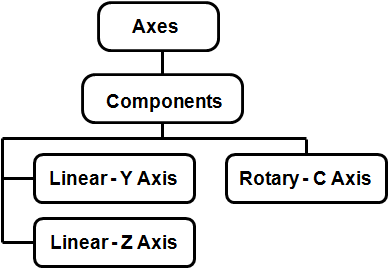
\includegraphics[width=.5\textwidth]{figures/axes-example-two-linear-one-rotary.png}
  \caption{Axes Example with Two Linear Axes and One Rotary Axis}
  \label{fig:axes-example-two-linear-one-rotary}
\end{figure}

\FloatBarrier

\subsubsection{Linear}

A \gls{linear} axis represents the movement of a physical piece of equipment, or a portion of the equipment, in a straight line.

Movement may be either in a positive or negative direction.

\gls{linear} type axes \must be identified using a value for the name attribute as X, Y, or Z with numbers appended for additional axes in the same plane.  Additional linear axes are often referred to as U, V, and W.   However, MTConnect defines the secondary axes to X, Y, and Z as X2, Y2, and Z2.

If the piece of equipment is unable to provide information associated with the \gls{name} attribute, then the \gls{nativename} attribute \must be included to identify the axis.

\subsubsection{Rotary}

A \gls{rotary} axis represents any non-linear or rotary movement of a physical piece of equipment or a portion of the equipment.

\gls{rotary} type axes \must be identified using a value for the \gls{name} attribute as A, B, and C for axes that rotate around the X, Y, and Z axes respectively.  As with the \gls{linear} axes, a number \must be appended for additional axes in the same plane (C, C2, C3, C4, ...).

If the piece of equipment is unable to provide information associated with the \gls{name} attribute, then the \gls{nativename} attribute \must be included to identify the axis.

An axis whose function is to provide rotary motion may function as a continuous rotation (\gls{spindle value} mode), continuous-path contour rotary motion (\gls{contour value} mode), or positioning (\gls{index value} mode) to discrete rotary positions.   As such, a \gls{rotary} type axis \should specify a \gls{rotarymode event} data item identifying the operating mode of the axis: \gls{spindle value}, \gls{index value}, or \gls{contour value}.

\paragraph{Chuck}\mbox{}

\gls{chuck component} is an XML container that provides the information about a mechanism that holds a part or stock material in place.   It may also represent the information about any other type mechanism that holds items in place within a piece of equipment.

The operation of a \gls{chuck component} when represented as a \gls{component} element is defined by \gls{chuckstate event}. The value of \gls{chuckstate event} \must be \gls{open value}, \gls{closed value}, or \gls{unlatched value}.

\gls{chuck component} may be used in the \gls{mtconnectdevices} document as either a \gls{lower level} component or as a \gls{composition} element of a parent \gls{component} element.

\subsection{Controller}

\gls{controller} is a \gls{top level} container that organizes information for an intelligent part of a piece of equipment that monitors and calculates information to alter the operating conditions of the equipment.  Typical types of controllers for a piece of equipment include CNC (Computer Numerical Control), PAC (Programmable Automation Control), IPC (Industrialized Computer), or IC (Imbedded Computer).

\gls{controller} is a component that organizes and provides information regarding the execution of a control program(s), the mode of operation of the piece of equipment, and fault information regarding the operation of the equipment.

\begin{note}
Note: MTConnect Version 1.1.0 and later implementations \should use a \gls{lower level} \gls{component} element called \gls{path} to represent an individual tool path or other independent function within a \gls{controller} element.  When the \gls{controller} element is capable of executing more than one simultaneous and independent programs, the implementation \must specify a \gls{lower level} \gls{path} element representing each of the independent functions of the \gls{controller}.

\end{note}

\subsubsection{Path}

\gls{path} is an XML container that represents the information for an independent operation or function within a \gls{controller}.  For many types of equipment, \gls{path} represents a set of \gls{axes}, one or more Program elements, and the data associated with the motion of a control point as it moves through space.   However, it \may also represent any independent function within a \gls{controller} that has unique data associated with that function.

\gls{path} \should provide an \gls{execution event} data item to define the operational state of the \gls{controller} component of the piece of equipment.

If the \gls{controller} is capable of performing more than one independent operation or function simultaneously, a separate \gls{path} component \must be used to organize the data associated with each independent operation or function.

\subsection{Systems}

\gls{systems} is a \gls{top level} XML container that provides structure for the information describing one or more \gls{lower level} functional systems that perform as discrete operating modules of the equipment or provide utility type services to support the operation of the equipment. These systems are required for the piece of equipment to perform its intended function and are permanently integrated into the piece of equipment.

Since these systems operate as separate functional units, they are represented in the \gls{mtconnectdevices} XML document as individual \gls{lower level} \gls{component} elements of \gls{systems} based on the function or service provided. 

\subsubsection{Hydraulic System}

\gls{hydraulic} is an XML container that represents the information for a system comprised of all the parts involved in moving and distributing pressurized liquid throughout the piece of equipment.

\subsubsection{Pneumatic System}

\gls{pneumatic} is an XML container that represents the information for a system comprised of all the parts involved in moving and distributing pressurized gas throughout the piece of equipment. 

\subsubsection{Coolant System}

\gls{coolant} is an XML container that represents the information for a system comprised of all the parts involved in distribution and management of fluids that remove heat from a piece of equipment.

\subsubsection{Lubrication System}

\gls{lubrication} is an XML container that represents the information for a system comprised of all the parts involved in distribution and management of fluids used to lubricate portions of the piece of equipment.

\subsubsection{Electric System}

\gls{electric} is an XML container that represents the information for the main power supply for device piece of equipment and the distribution of that power throughout the equipment.  The electric system will provide all the data with regard to electric current, voltage, frequency, etc. that applies to the piece of equipment as a functional unit.   Data regarding electric power that is specific to a \gls{component} will be reported as \glspl{data entity} for that specific \gls{component}.

\subsubsection{Enclosure System}

\gls{enclosure} is an XML container that represents the information for a structure used to contain or isolate a piece of equipment or area.  The \gls{enclosure} system may provide information regarding access to the internal components of a piece of equipment or the conditions within the enclosure.   For example, \gls{door component} may be defined as a \gls{lower level} \gls{component} or \gls{composition} element of the \gls{enclosure} system.

\subsubsection{Protective System}

\gls{protective} is an XML container that represents the information for those functions that detect or prevent harm or damage to equipment or personnel.  \gls{protective} does not include the information relating to the \gls{enclosure} system.

\subsubsection{ProcessPower System}

\gls{processpower} is an XML container that represents the information for a power source associated with a piece of equipment that supplies energy to the manufacturing process separate from the \gls{electric} system.  For example, this could be the power source for an EDM machining process, an electroplating line, or a welding system.  

\subsubsection{Feeder System}

\gls{feeder} is an XML container that represents the information for a system that manages the delivery of materials within a piece of equipment.   For example, this could describe the wire delivery system for an EDM or welding process; conveying system or pump and valve system distributing material to a blending station; or a fuel delivery system feeding a furnace.  

\subsubsection{Dielectric System}

\gls{dielectric} is an XML container that represents the information for a system that manages a chemical mixture used in a manufacturing process being performed at that piece of equipment.  For example, this could describe the dielectric system for an EDM process or the chemical bath used in a plating process. 

\DIFaddbegin \subsubsection{\DIFadd{EndEffector System}}

\DIFadd{\gls{endeffector} is an XML container that represents the information for those functions that form the last link segment of a robot. It is the part of the robot that interacts with the manufacturing process.
}\DIFaddend \subsection{Auxiliaries}

\gls{auxiliaries} is a \gls{top level} XML container that provides structure for the information describing one or more \gls{lower level} functional systems that provide supplementary or additional capabilities for the operation of a piece of equipment.  These systems extend the capabilities of a piece of equipment, but are not required for the equipment to function.

Since these systems operate as independent units or are only temporarily associated with a piece of equipment, they are represented in the \gls{mtconnectdevices} XML document as individual \gls{lower level} \gls{component} elements of \gls{auxiliaries} based on the function or service provided to the equipment.

\subsubsection{Loader System}

\gls{loader} is an XML container that represents the information for a unit comprised of all the parts involved in moving and distributing materials, parts, tooling, and other items to or from a piece of equipment.

\subsubsection{WasteDisposal System}

\gls{wastedisposal} is an XML container that represents the information for a unit comprised of all the parts involved in removing manufacturing byproducts from a piece of equipment.

\subsubsection{ToolingDelivery System}

\gls{toolingdelivery} is an XML container that represents the information for a unit involved in managing, positioning, storing, and delivering tooling within a piece of equipment.

\subsubsection{BarFeeder System}

\gls{barfeeder} is an XML container that represents the information for a unit involved in delivering bar stock to a piece of equipment.

\subsubsection{Environmental System}

\gls{environmental} is an XML container that represents the information for a unit or function involved in monitoring, managing, or conditioning the environment around or within a piece of equipment.

\subsubsection{Sensor System}

\gls{sensor} is a XML container that represents the information for a piece of equipment that responds to a physical stimulus and transmits a resulting impulse or value from a sensing unit.   When modeled as a component of \gls{auxiliaries}, sensor \should represent an integrated \gls{sensor unit} system that provides signal processing, conversion, and communications.  A \gls{sensor unit} may have multiple \glspl{sensing element}; each representing the data for a variety of measured values.  See \sect{Sensor Unit} for more details on \gls{sensor unit}.

\begin{note}
Note:  If modeling an individual sensor, then sensor should be associated with the component that the measured value is most closely associated.  See \sect{Sensor}.
\end{note}

\DIFaddbegin \subsubsection{\DIFadd{Deposition System}}

\DIFadd{\gls{deposition} is an XML container that represents the information for a system that manages the addition of material or state change of material being performed in an additive manufacturing process.  For example, this could describe the portion of a piece of equipment that manages a material extrusion process or a vat polymerization process.
}


\DIFaddend \subsection{Resources}

\gls{resources} is a \gls{top level} XML container that groups items that support the operation of a piece of equipment.   \gls{resources} also represents materials or other items consumed, transformed, or used for production of parts, materials, or other types of goods by a piece of equipment.

\subsubsection{Materials}

\gls{materials} is an XML container that provides information about materials or other items consumed or used by the piece of equipment for production of parts, materials, or other types of goods.  \gls{materials} also represents parts or part stock that are present at a piece of equipment or location to which work is applied to transform the part or stock material into a more finished state. 

\paragraph{Stock}\mbox{}

\gls{stock} is an XML container that represents the information for the material that is used in a manufacturing process and to which work is applied in a machine or piece of equipment to produce parts.

\gls{stock} may be either a continuous piece of material from which multiple parts may be produced or it may be a discrete piece of material that will be made into a part or a set of parts.

\subsection{Interfaces}

\gls{interfaces component} is a \gls{top level} XML \gls{structural element} in the \gls{mtconnectdevices} XML document.  \gls{interfaces component} organizes the information provided by a piece of equipment used to coordinate activities with other pieces of equipment.   As such, \gls{interfaces component} represents the inter-device communication information between a piece of equipment and other pieces of equipment.

See \citetitle{MTCPart5} for detailed information on \gls{interfaces component}.

\subsection{Other Components}

While most component elements \should be modeled in a specific manner, there are some types of component elements that are used ubiquitously in equipment and \may be associated with any number of different types of parent component elements.

These components \may be modeled as \gls{lower level} components of the Parent Element.

\subsubsection{Actuator}

\gls{actuator} is an XML container that represents the information for an apparatus for moving or controlling a mechanism or system.  It takes energy usually provided by air, electric current, or liquid and converts the energy into some kind of motion.  

\subsubsection{Door}

\gls{door component} is an XML container that represents the information for a mechanical mechanism or closure that can cover, for example, a physical access portal into a piece of equipment.  The closure can be opened or closed to allow or restrict access to other parts of the equipment.

When \gls{door component} is represented as a \gls{component}, it \must have a data item called \gls{doorstate event} to indicate if the door is \gls{open value}, \gls{closed value}, or \gls{unlatched value}.  A \gls{component} \may contain multiple \gls{door component} components.

\subsubsection{Sensor}
\label{sec:Sensor}

\gls{sensor} is a XML container that represents the information for a piece of equipment that responds to a physical stimulus and transmits a resulting impulse or value.  If modeling individual sensors, then sensor should be associated with the component that the measured value is most closely associated.   

See \sect{Sensors} for more details on the use of \gls{sensor}.

\section{Composition Type Structural Elements}
\label{sec:Composition Type Structural Elements}

\gls{composition} \glspl{structural element} are used to describe the lowest level physical building blocks of a piece of equipment contained within a \gls{component}. By referencing a specific \gls{composition} element, further clarification and meaning to data associated with a specific \gls{component} can be achieved.

Both \gls{component} and \gls{composition} elements are \gls{lower level} child \gls{component} XML elements representing the sub-parts of the parent \gls{component}.  However, there are distinct differences between \gls{component} and \gls{composition} type elements.

\gls{component} elements may be further defined with \gls{lower level} \gls{component} elements and may have associated \glspl{data entity}.

\gls{composition} elements represent the lowest level physical part of a piece of equipment.  They \mustnot be further defined with \gls{lower level} \gls{component} elements and they \mustnot have \glspl{data entity} directly associated with them.   They do provide additional information that can be used to enhance the specificity of \glspl{data entity} associated with the parent \gls{component}.

\tbl{elements-lowerlevel-for-composition} defines \gls{composition} type elements that are currently available to describe sub-parts of a \gls{component} element.

\tabulinesep = 5pt
\begin{longtabu} to \textwidth {
    |l|X[3l]|}
\caption{Composition type Elements} \label{table:elements-lowerlevel-for-composition} \\

\hline
Element Type & Description\\
\hline
\endfirsthead

\hline
\multicolumn{2}{|c|}{Continuation of Table \ref{table:elements-lowerlevel-for-composition}}\\
\hline
Element Type & Description\\
\hline
\endhead

\gls{actuator type} & \glsentrydesc{actuator type} \\ \hline

\gls{amplifier} & \glsentrydesc{amplifier} \\ \hline

\gls{ballscrew} & \glsentrydesc{ballscrew} \\ \hline

\gls{belt} & \glsentrydesc{belt} \\ \hline

\gls{brake} & \glsentrydesc{brake} \\ \hline

\gls{chopper} & \glsentrydesc{chopper} \\ \hline

\gls{circuitbreaker} & \glsentrydesc{circuitbreaker} \\ \hline

\gls{chain} & \glsentrydesc{chain} \\ \hline

\gls{chuck} & \glsentrydesc{chuck} \\ \hline

\gls{chute} & \glsentrydesc{chute} \\ \hline

\gls{clamp} & \glsentrydesc{clamp} \\ \hline

\gls{compressor} & \glsentrydesc{compressor} \\ \hline

\gls{door} & \glsentrydesc{door} \\ \hline

\gls{drain} & \glsentrydesc{drain} \\ \hline

\gls{encoder} & \glsentrydesc{encoder} \\ \hline

\gls{fan} & \glsentrydesc{fan} \\ \hline

\gls{filter type} & \glsentrydesc{filter type} \\ \hline

\gls{gripper} & \glsentrydesc{gripper} \\ \hline

\gls{hopper} & \glsentrydesc{hopper} \\ \hline

\gls{motor} & \glsentrydesc{motor} \\ \hline

\gls{oil} & \glsentrydesc{oil} \\ \hline

\gls{pump} & \glsentrydesc{pump} \\ \hline

\gls{linearpositionfeedback} & \glsentrydesc{linearpositionfeedback} \\ \hline

\gls{powersupply} & \glsentrydesc{powersupply} \\ \hline

\gls{pulley} & \glsentrydesc{pulley} \\ \hline

\gls{sensingelement} & \glsentrydesc{sensingelement} \\ \hline

\gls{storagebattery} & \glsentrydesc{storagebattery} \\ \hline

\gls{switch} & \glsentrydesc{switch} \\ \hline

\gls{tank} & \glsentrydesc{tank} \\ \hline

\gls{tensioner} & \glsentrydesc{tensioner} \\ \hline

\gls{transformer} & \glsentrydesc{transformer} \\ \hline

\gls{valve} & \glsentrydesc{valve} \\ \hline

\gls{water} & \glsentrydesc{water} \\ \hline

\gls{wire} & \glsentrydesc{wire} \\ \hline



\DIFaddbegin \DIFadd{\gls{galvanomotor}
}&
\DIFadd{An electromechanical actuator that produces deflection of a beam of light or energy in response to electric current through its coil in a magnetic field. }\\
\hline

\DIFadd{\gls{vat}
}&
\DIFadd{A container for liquid or powdered materials }\\
\hline

\DIFadd{\gls{table}
}&
\DIFadd{A surface for holding an object or material }\\
\hline

\DIFadd{\gls{exposureunit}
}&
\DIFadd{A mechanism for emitting a type of radiation }\\
\hline

\DIFadd{\gls{reel}
}&
\DIFadd{A rotary storage unit for material }\\
\hline

\DIFadd{\gls{spreader}
}&
\DIFadd{A mechanism for flattening or spreading materials }\\
\hline

\DIFadd{\gls{extrusionunit}
}&
\DIFadd{A mechanism for dispensing liquid or powered materials }\\
\hline\DIFaddend \end{longtabu}

\begin{note}
Note:  As the MTConnect Standard evolves, more \gls{composition} types will be added.

\end{note}

\section {Data Entities for Device}
\label{sec:Data Entities for Device}

In the \gls{mtconnectdevices} XML document, \glspl{data entity} are XML elements that describe data that can be reported by a piece of equipment and are associated with \gls{device} and \gls{component} \glspl{structural element}.   While the \glspl{data entity} describe the data that can be reported by a piece of equipment in the \gls{mtconnectdevices} document, the actual data values are provided in the \gls{streams information model}.   See \citetitle{MTCPart3} for detail on the reported values.

Each \gls{data entity} \should be modeled in the \gls{mtconnectdevices} document such that it is associated with the \gls{structural element} that the reported data directly applies.

When \glspl{data entity} are associated with a \gls{structural element}, they are organized in a \gls{dataitems} XML element.   \gls{dataitems} is a container type XML element.  \gls{dataitems} provides the structure for organizing individual \gls{dataitem} elements that represent each Data Enitity. The \gls{dataitems} container is comprised of one or more \gls{dataitem} type XML element(s).

\gls{dataitem} describes specific types of \glspl{data entity} that represent a numeric value, a functioning state, or a health status reported by a piece of equipment.   \gls{dataitem} provides a detailed description for each \gls{data entity} that is reported; it defines the type of data being reported and an array of optional attributes that further describes that data.   The different types of \gls{dataitem} elements are defined in \sect{Listing of Data Items}.

\fig{data-entities-example-device} demonstrates the relationship between \glspl{data entity} (\gls{dataitem}) and the various \glspl{structural element} in the \gls{mtconnectdevices} XML document.    

\begin{figure}[ht]
  \centering
  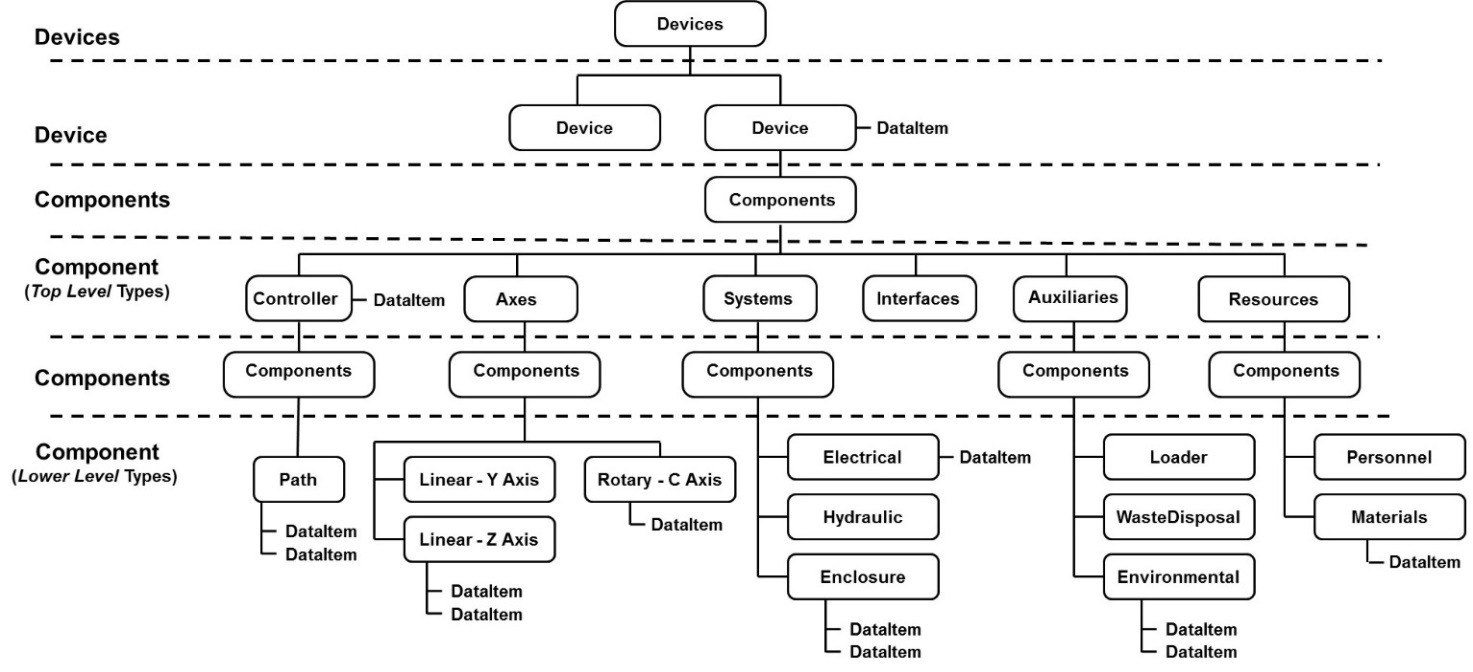
\includegraphics[width=.75\textwidth]{figures/data-entities-example-device.png}
  \caption{Example Data Entities for Device (DataItem)}
  \label{fig:data-entities-example-device}
\end{figure}

\subsection{DataItems}

The \gls{dataitems} XML element is the first, or highest, level container for the \glspl{data entity} associated with a \gls{device} or \gls{component} XML element.  \gls{dataitems} \must contain only \gls{dataitem} type elements.  \gls{dataitems} \must contain at least one \gls{dataitem} type element, but \may contain multiple \gls{dataitem} type elements.

\tabulinesep = 5pt
\begin{longtabu} to \textwidth {
    |l|X[3l]|X[0.75l]|}
\caption{MTConnect DataItems Element} \label{table:mtconnect-dataitems-element} \\

\hline
Element & Description & Occurrence \\
\hline
\endfirsthead

\hline
\multicolumn{3}{|c|}{Continuation of Table \ref{table:mtconnect-dataitems-element}}\\
\hline
Element & Description & Occurrence \\
\hline
\endhead

\gls{dataitems}
&
\glsentrydesc{dataitems}
\newline Only one \gls{dataitems} container \MUST appear for each \gls{structural element} in the XML document.
&
0..1 \\
\hline


\end{longtabu}

\subsection{DataItem}

A \gls{dataitem} XML element represents each \gls{data entity} that \may be reported by a piece of equipment through an \gls{agent}.   \gls{dataitem} provides a detailed description for each \gls{data entity} that is reported and defines the type of data being reported along with an array of optional attributes that further define that data.  XML elements representing \gls{dataitem} will include elements such as \gls{temperature sample}, \gls{pressure sample}, and \gls{velocity sample}. 

\tabulinesep = 5pt
\begin{longtabu} to \textwidth {
    |l|X[3l]|X[0.75l]|}
\caption{MTConnect Dataitem Element} \label{table:mtconnect-dataitem-element} \\

\hline
Element & Description & Occurrence \\
\hline
\endfirsthead

\hline
\multicolumn{3}{|c|}{Continuation of Table \ref{table:mtconnect-dataitem-element}}\\
\hline
Element & Description & Occurrence \\
\hline
\endhead

\gls{dataitem}	
&
\glsentrydesc{dataitem}
&
1..* \\
\hline


\end{longtabu}


\subsubsection{XML Schema Structure for DataItem}

\fig{dataitem-schema-diagram} represents the structure of a \gls{dataitem} XML element showing the attributes defined for \gls{dataitem} and the elements that may be associated with \gls{dataitem} type XML elements.

\begin{figure}[ht]
  \centering
  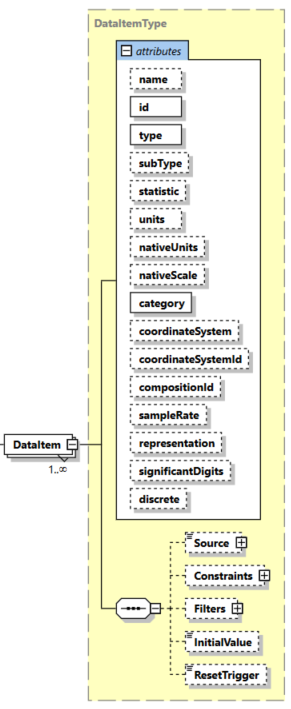
\includegraphics[width=.45\textwidth]{figures/dataitem-schema-diagram.png}
  \caption{DataItem Diagram}
  \label{fig:dataitem-schema-diagram}
\end{figure}
\FloatBarrier

\subsubsection{Attributes for DataItem}
\label{sec:Attributes for DataItem}

\tbl{attributes-for-dataitem} lists the attributes defined to provide information for a \gls{dataitem} type XML element.  

\gls{dataitem} \must specify the type of data being reported, the id of the \gls{dataitem}, and the \gls{category} of the \gls{dataitem}.  

\tabulinesep = 5pt
\begin{longtabu} to \textwidth {
    |l|X[3l]|X[0.75l]|}
\caption{Attributes for DataItem} \label{table:attributes-for-dataitem} \\

\hline
Attribute & Description & Occurrence \\
\hline
\endfirsthead

\hline
\multicolumn{3}{|c|}{Continuation of Table \ref{table:attributes-for-dataitem}}\\
\hline
Attribute & Description & Occurrence \\
\hline
\endhead

\gls{name}
&
The name of the data item.
\newline \gls{name} is provided as an additional human readable identifier for this data item in addition to the \gls{id}.
\newline \gls{name} is an optional attribute and will be implementation dependent.
\newline An \gls{nmtoken} XML type.
&
0..1 \\
\hline

\gls{id} 
&
\glsentrydesc{id}
\newline \gls{id} is a required attribute.
\newline The \gls{id} attribute \MUST be unique within the
\gls{mtconnectdevices} document.
\newline An XML ID-type.
&
1 \\
\hline

\gls{type}
&
The type of data being measured.
\newline \gls{type} is a required attribute.
\newline Examples of types are \gls{position sample}, \gls{velocity sample}, \gls{angle sample}, \gls{block event}, and \gls{rotaryvelocity sample}.
&
1 \\
\hline

\gls{subtype}
&
A sub-categorization of the data item \gls{type}.
\newline \gls{subtype} is an optional attribute.
\newline For example, the \gls{subtype} of \gls{position sample} can be \gls{actual subtype} or \gls{commanded subtype}.
\newline Not all \gls{type} attributes have a \gls{subtype}. 
&
0..1 \\
\hline

\gls{statistic}
&
Describes the type of statistical calculation performed on a series of data samples to provide the reported data value.
\newline \gls{statistic} is an optional attribute.
\newline Examples of \gls{statistic} are \gls{average}, \gls{minimum value}, \gls{maximum value}, \gls{rootmeansquare}, \gls{range}, \gls{median}, \gls{mode}, and \gls{standarddeviation}.
&
0..1 \\
\hline

\gls{units}
&
The unit of measurement for the reported value of the data item.
\newline \gls{units} is an optional attribute.
\newline Data items in the \gls{sample} category \MUST report the standard units for the measured values.
\newline See \sect{units Attribute for DataItem} for a list of available standard units identified in the MTConnect Standard.
&
0..1 \\
\hline

\gls{nativeunits}
&
The native units of measurement for the reported value of the data item.
\newline \gls{nativeunits} is an optional attribute.
\newline See \sect{nativeUnits Attribute for DataItem} for a list of available native units identified in the MTConnect Standard.
&
0..1 \\
\hline

\gls{nativescale}
&
The \gls{nativeunits} may not be scaled to directly represent the original measured value. \gls{nativescale} \MAY be used to convert the reported value to represent the original measured value.
\newline \gls{nativescale} is an optional attribute.
\newline As an example, the \gls{nativeunits} may be reported as
\gls{gallonperminute}. The measured value may actually be in 1000  \gls{gallonperminute}. The value of the reported data \MAY be divided by the \gls{nativescale} to convert the reported value to its original measured value and units.
\newline If provided, the value \MUST be numeric.
&
0..1 \\
\hline

\gls{category}
&
\glsentrydesc{category}
\newline \gls{category} is a required attribute.
\newline The available options are \gls{sample}, \gls{event}, or \gls{condition}.
&
1 \\
\hline

\gls{coordinatesystem}
&
\glsentrydesc{coordinatesystem}
\newline \gls{coordinatesystem} is an optional attribute.
\newline The available values for \gls{coordinatesystem} are \gls{work} and \gls{machine}.
&
0..1 \\
\hline

\gls{compositionid}
&
The identifier attribute of the \gls{composition} element that the reported data is most closely associated.
\newline \gls{compositionid} is an optional attribute. 
&
0..1 \\
\hline

\gls{samplerate}
&
The rate at which successive samples of a data item are recorded by a piece of equipment.
\newline \gls{samplerate} is an optional attribute.
\newline \gls{samplerate} is expressed in terms of samples per second.
\newline If the \gls{samplerate} is smaller than one, the number can be represented as a floating point number.
\newline For example, a rate 1 per 10 seconds would be 0.1
&
0..1\\
\hline

\gls{representation}
&
Description of a means to interpret data consisting of multiple data points or as a single value.
\newline \gls{representation} is an optional attribute.
\newline \gls{representation} defines the unique format for each set of data.
\newline \gls{representation} for \gls{timeseries representation}, \gls{discrete representation} \DIFdelbegin \DIFdel{ and }\DIFdelend \DIFaddbegin \DIFadd{, \gls{dataset}, and }\DIFaddend \gls{value representation} are defined in \sect{representation Attribute for DataItem}.
\newline If \gls{representation} is not specified, it \MUST be determined to be \gls{value representation}.
\DIFaddend &
0..1 \\
\hline

\gls{significantdigits}
&
The number of significant digits in the reported value.
\newline \gls{significantdigits} is an optional attribute.
\newline This \SHOULD be specified for all numeric values.
&
0..1 \\
\hline



\DIFaddbegin \DIFadd{\gls{discrete}
}&
\DIFadd{An indication signifying whether each value reported for the \gls{data entity} is significant and whether duplicate values are to be suppressed.
}\newline \DIFadd{The value defined \MUST be either \gls{true removed} or \gls{false removed} - an XML boolean type.
}\newline \DIFadd{\gls{true removed} indicates that each update to the \gls{data entity}'s value is significant and duplicate values \MUSTNOT be suppressed.
}\newline \DIFadd{\gls{false removed} indicates that duplicated values \MUST be suppressed.
}\newline \DIFadd{If a value is not defined for \gls{discrete}, the default value \MUST be \gls{false removed}.
}&
\DIFadd{0..1 }\\
\hline\DIFaddend \end{longtabu}

\paragraph{name Attribute for DataItem}\mbox{}

The attribute \gls{name} is provided as an additional human readable identifier for a data item.  It is not required and is implementation dependent.

\paragraph{id Attribute for DataItem}\mbox{}

Each \gls{dataitem} element \must be identified with an \gls{id}.   The \gls{id} attribute \must be unique across the entire \gls{mtconnectdevices} document for a piece of equipment, including the identifiers for all \glspl{structural element}.  This unique \gls{id} provides the information required by a client software application to uniquely identify each \gls{data entity}.

For example, an XML document may provide three different \glspl{data entity} representing the position of the axes on a machine (x axis position, y axis position, and z axis position).  All three may be modeled in the XML document as Position type data items for the \gls{axes} components.  The unique \gls{id} allows the client software application to distinguish the data for each of the axes.

\paragraph{type and Subtype Attributes for DataItem}\mbox{}

The attribute \gls{type} specifies the kind of data that is represented by the data item.

The attribute \gls{type} \must be specified for every data item.

A data item \may further qualify the data being reported by specifying a \gls{subtype}.  \gls{subtype} is required for certain data item \glspl{type}.  For example, \gls{position sample} has the \gls{subtype} of \gls{actual subtype} and \gls{programmed subtype}.  Both data values can be represented in the document as two separate and different \gls{dataitem} XML elements - \gls{position sample} with \gls{subtype} \gls{actual subtype} and \gls{position sample} with \gls{subtype} \gls{programmed subtype}.

The \gls{type} and \gls{subtype} \should be used to further identify the meaning of the \gls{dataitem} associated with a \gls{component} element when a \gls{subtype} is applicable.  There \shouldnot be more than one \gls{dataitem} with the same \gls{type}, \gls{subtype}, and \gls{compositionid} within a \gls{component} element.

\sect{Listing of Data Items} provides a detailed listing of the data item \gls{type} and \gls{subtype} elements defined for each \gls{category} of data item available for a piece of equipment: \gls{sample category}, \gls{event category}, and \gls{condition category}.

\paragraph{statistic Attribute for DataItem}\mbox{}

A piece of equipment may further process some data types using a statistical calculation like average, mean, or square root.  In this case, the \gls{statistic} attribute \may be used to indicate how the data was processed.  

\gls{statistic} may be defined for any \gls{sample category} type \gls{dataitem}.   All statistic data is reported in the standard units of the \gls{dataitem}.

\gls{statistic} data is always the result of a calculation using data that has been measured over a specified period of time. 

The value of \gls{statistic} may be periodically reset.   When a piece of equipment reports a \gls{dataitem} with a value that is a \gls{statistic}, the information provided in the XML document for that \gls{data entity} \must include an additional attribute called \gls{duration}.   The attribute \gls{duration} defines the period of time over which the \gls{statistic} has been calculated.   See \citetitle{MTCPart3} for more information about \gls{duration}.

\tbl{dataitem-attribute-statistic-type} shows the \gls{statistic} calculations that can be defined for a \gls{dataitem}.

\tabulinesep = 5pt
\begin{longtabu} to \textwidth {
    |l|X[3l]|}
\caption{DataItem attribute statistic type} \label{table:dataitem-attribute-statistic-type} \\

\hline
Statistic & Description\\
\hline
\endfirsthead

\hline
\multicolumn{2}{|c|}{Continuation of Table \ref{table:dataitem-attribute-statistic-type}}\\
\hline
Statistic & Description\\
\hline
\endhead

\gls{average} & \glsentrydesc{average} \\ \hline

\gls{kurtosis} & \glsentrydesc{kurtosis} \\ \hline

\gls{maximum value} &
Maximum or peak value recorded for the data item during the calculation period.\\ \hline

\gls{median} & \glsentrydesc{median} \\ \hline

\gls{minimum value} &
Minimum value recorded for the data item during the calculation period.\\ \hline

\gls{mode} & \glsentrydesc{mode} \\ \hline

\gls{range} & \glsentrydesc{range} \\ \hline

\gls{rootmeansquare} & \glsentrydesc{rootmeansquare} \\ \hline

\gls{standarddeviation} & \glsentrydesc{standarddeviation} \\ \hline

\end{longtabu}


\pagebreak

\paragraph{units Attribute for DataItem}\label{sec:units Attribute for DataItem}\mbox{}

\tbl{dataitem-attribute-units-type} lists the units that are defined as the standard unit of measure for each type of \gls{dataitem}.  All \gls{sample category} type data items \must report data values in standard units.     

\tabulinesep = 5pt
\begin{longtabu} to \textwidth {
    |l|X[3l]|}
\caption{DataItem attribute units type} \label{table:dataitem-attribute-units-type} \\

\hline
Units & Description\\
\hline
\endfirsthead

\hline
\multicolumn{2}{|c|}{Continuation of Table \ref{table:dataitem-attribute-units-type}}\\
\hline
Units & Description\\
\hline
\endhead

\gls{ampere} & \glsentrydesc{ampere} \\ \hline

\gls{celsius} & \glsentrydesc{celsius} \\ \hline

\gls{count} & \glsentrydesc{count} \\ \hline

\gls{decibel} & \glsentrydesc{decibel} \\ \hline

\gls{degree} & \glsentrydesc{degree} \\ \hline

\gls{degreepersecond} & \glsentrydesc{degreepersecond} \\ \hline

\gls{degreepersecondsquared} & \glsentrydesc{degreepersecondsquared} \\ \hline

\gls{hertz} & \glsentrydesc{hertz} \\ \hline

\gls{joule} & \glsentrydesc{joule} \\ \hline

\gls{kilogram} & \glsentrydesc{kilogram} \\ \hline

\gls{liter} & \glsentrydesc{liter} \\ \hline

\gls{literpersecond} & \glsentrydesc{literpersecond} \\ \hline

\gls{microradian} & \glsentrydesc{microradian} \\ \hline

\gls{millimeter} & \glsentrydesc{millimeter} \\ \hline

\gls{millimeterpersecond} & \glsentrydesc{millimeterpersecond} \\ \hline

\gls{millimeterpersecondsquared} & \glsentrydesc{millimeterpersecondsquared} \\ \hline

\gls{millimeter3d} & \glsentrydesc{millimeter3d} \\ \hline

\gls{newton} & \glsentrydesc{newton} \\ \hline

\gls{newtonmeter} & \glsentrydesc{newtonmeter} \\ \hline

\gls{ohm} & \glsentrydesc{ohm} \\ \hline

\gls{pascal} & \glsentrydesc{pascal} \\ \hline

\gls{percent} & \glsentrydesc{percent} \\ \hline

\gls{ph sample}
&
A measure of the acidity or alkalinity of a solution. \\ \hline

\gls{revolutionperminute} & \glsentrydesc{revolutionperminute} \\ \hline

\gls{second} & \glsentrydesc{second} \\ \hline

\gls{siemenspermeter} & \glsentrydesc{siemenspermeter} \\ \hline

\gls{volt} & \glsentrydesc{volt} \\ \hline

\gls{voltampere sample} & Volt-Ampere (VA) \\ \hline

\gls{voltamperereactive sample} & Volt-Ampere Reactive (VAR) \\ \hline

\gls{watt} & \glsentrydesc{watt} \\ \hline

\gls{wattsecond} & \glsentrydesc{wattsecond} \\ \hline



\DIFaddbegin \DIFadd{\gls{cubicmillimeter}
}&
\DIFadd{Geometric volume in millimeters }\\
\hline

\DIFadd{\gls{cubicmillimeterpersecond}
}&
\DIFadd{Change of geometric volume per second }\\
\hline

\DIFadd{\gls{cubicmillimeterpersecondsquared}
}&
\DIFadd{Change in geometric volume per second squared }\\
\hline

\DIFadd{\gls{milligram}
}&
\DIFadd{Milligram  }\\
\hline

\DIFadd{\gls{milligrampercubicmillimeter}
}&
\DIFadd{Milligram per cubic millimeter   }\\
\hline

\DIFadd{\gls{milliliter}
}&
\DIFadd{Milliliter   }\\
\hline

\DIFadd{\gls{millimeterperrevolution}
}&
\DIFadd{\glsentrydesc{millimeterperrevolution}
 }\\
\hline\DIFaddend \end{longtabu}

\paragraph{nativeUnits Attribute for DataItem}\label{sec:nativeUnits Attribute for DataItem}\mbox{}

The \gls{nativeunits} attribute provides additional information about the original measured value for a \gls{data entity} reported by a piece of equipment.  \gls{nativeunits} \may be specified to provide additional information about the data if the units of the measured value supplied by the piece of equipment differ from the value provided for that data when converted to standard units.

\tbl{dataitem-attribute-nativeunits-type} defines the \gls{nativeunits} currently supported by the \gls{mtconnectdevices} XML document:

\tabulinesep = 5pt
\begin{longtabu} to \textwidth {
    |l|X[3l]|}
\caption{DataItem attribute nativeunits type} \label{table:dataitem-attribute-nativeunits-type} \\

\hline
Native Units & Description\\
\hline
\endfirsthead

\hline
\multicolumn{2}{|c|}{Continuation of Table \ref{table:dataitem-attribute-nativeunits-type}}\\
\hline
Native Units & Description\\
\hline
\endhead

\gls{centipoise} & \glsentrydesc{centipoise} \\ \hline

\gls{degreeperminute} & \glsentrydesc{degreeperminute} \\ \hline

\gls{fahrenheit} & \glsentrydesc{fahrenheit} \\ \hline

\gls{foot} & \glsentrydesc{foot} \\ \hline

\gls{footperminute} & \glsentrydesc{footperminute} \\ \hline

\gls{footpersecond} & \glsentrydesc{footpersecond} \\ \hline

\gls{footpersecondsquared} & \glsentrydesc{footpersecondsquared} \\ \hline

\gls{foot3d} & \glsentrydesc{foot3d} \\ \hline

\gls{gallonperminute} & \glsentrydesc{gallonperminute} \\ \hline

\gls{inch} & \glsentrydesc{inch} \\ \hline

\gls{inchperminute} & \glsentrydesc{inchperminute} \\ \hline

\gls{inchpersecond} & \glsentrydesc{inchpersecond} \\ \hline

\gls{inchpersecondsquared} & \glsentrydesc{inchpersecondsquared} \\ \hline

\gls{inch3d} & \glsentrydesc{inch3d} \\ \hline

\gls{inchpound} & \glsentrydesc{inchpound} \\ \hline

\gls{kelvin} & \glsentrydesc{kelvin} \\ \hline

\gls{kilowatt} & \glsentrydesc{kilowatt} \\ \hline

\gls{kilowatthour} & \glsentrydesc{kilowatthour} \\ \hline

\gls{liter} & \glsentrydesc{liter} \\ \hline

\gls{literperminute} & \glsentrydesc{literperminute} \\ \hline

\gls{millimeterperminute} & \glsentrydesc{millimeterperminute} \\ \hline

\gls{pound} & \glsentrydesc{pound} \\ \hline

\gls{poundperinchsquared} & \glsentrydesc{poundperinchsquared} \\ \hline

\gls{radian} & \glsentrydesc{radian} \\ \hline

\gls{radianpersecond} & \glsentrydesc{radianpersecondsquared} \\ \hline

\gls{radianpersecondsquared} & \glsentrydesc{radianpersecondsquared} \\ \hline

\gls{radianperminute} & \glsentrydesc{radianperminute} \\ \hline

\gls{revolutionpersecond} & \glsentrydesc{revolutionpersecond} \\ \hline

\gls{other} & \glsentrydesc{other} \\ \hline



\DIFaddbegin \DIFadd{\gls{hour}
}&
\DIFadd{A measurement of time in hours }\\
\hline

\DIFadd{\gls{minute}
}&
\DIFadd{A measurement of time in minutes }\\
\hline\DIFaddend \end{longtabu}

\pagebreak

\paragraph{nativeScale Attribute for DataItem}\mbox{}

The units of measure for some measured values may be different from the \gls{nativeunits} defined in \sect{category Attribute for DataItem}.   In the cases where the units of measure use a different weighting or range than is provided by \gls{nativeunits}, the \gls{nativescale} attribute can be used to define the original units of measure.

As an example, a velocity measured in units of 100 ft/min can be represented as \cfont{nativeUnits="FEET/MINUTE"} and \cfont{nativeScale="100"}. 

\paragraph{category Attribute for DataItem}
\label{sec:category Attribute for DataItem}\mbox{}

Many \gls{dataitem} types provide two forms of data, a value (reported as either a \gls{sample category} or \gls{event category} category) and a health status (reported as a \gls{condition category} category).  Therefore, each occurrence of a \gls{dataitem} in the XML document \must report a \gls{category} attribute.  This \gls{category} attribute provides the information required by a client software application to determine the specific meaning of the data provided.

Each \gls{data entity} provided by a piece of equipment \must be identified with one of the following:

\gls{sample category}

\tab A \gls{sample category} is the reading of the value of a continuously variable or analog data value.  A continuous value can be measured at any point-in-time and will always produce a result.  An example of a continuous data value is the position of the \gls{linear} X Axis.   

The data provided for a \gls{sample category} category data item is always a floating point number or integers that have an infinite number of possible values.  This is different from a state or discrete type data item that has a limited number of possible values.  A data item of category \gls{sample category} \must also provide the \gls{units} attribute.

\gls{event category}

\tab An \gls{event category} is a data item representing a discrete piece of information from the piece of equipment.  \gls{event category} does not have intermediate values that vary over time, as does \gls{sample category}.   An \gls{event category} is information that, when provided at any specific point in time, represents the current state of the piece of equipment.

There are two types of \gls{event category}: those representing state, with two or more discrete values, and those representing messages that contain plain text data.

An example of a state type \gls{event category} is the value of the data item \gls{doorstate event}, which can be \gls{open value}, \gls{closed value}, or \gls{unlatched value}.   (Note:  No other values are valid to represent the value of \gls{doorstate event}.)

An example of a message type \gls{event category} is the value for a data item \gls{program event}.  The value representing \gls{program event} can be any valid string of characters.

\gls{condition category}

\tab A \gls{condition category} is a data item that communicates information about the health of a piece of equipment and its ability to function.  A valid value for a data item in the category \gls{condition category} can be one of \gls{normal}, \gls{warning}, or \gls{fault}.

A data item of category \gls{condition category} \may report multiple values (\gls{condition category}) at one time whereas a data item of category \gls{sample category} or \gls{event category} can only have a single value at any one point in time.

\paragraph{coordinateSystem Attribute for DataItem}\mbox{}

The values reported by a piece of equipment for some types of data will be associated to a specific positioning measurement system used by the equipment.  The \gls{coordinatesystem} attribute \may be used to specify the coordinate system used for the measured value.

The \gls{coordinatesystem} attribute is used by a client software application to interpret the spatial relationship between values reported by a piece of equipment.

If \gls{coordinatesystem} is not provided, all values representing positional data for \gls{axes} \must be interpreted using the \gls{machine} coordinate system and all values representing positional data for \gls{path} \must be interpreted using the \gls{work} coordinate system.

\tbl{dataitem-attribute-coordinatesystem} defines the types of \gls{coordinatesystem} currently supported by the \gls{mtconnectdevices} XML document:

\tabulinesep = 5pt
\begin{longtabu} to \textwidth {
    |l|X[3l]|}
\caption{DataItem attribute coordinateSystem} \label{table:dataitem-attribute-coordinatesystem} \\

\hline
Coordinate System & Description\\
\hline
\endfirsthead

\hline
\multicolumn{2}{|c|}{Continuation of Table \ref{table:dataitem-attribute-coordinatesystem}}\\
\hline
Coordinate System & Description\\
\hline
\endhead

\gls{machine}
&
\glsentrydesc{machine} \\ 
\hline

\gls{work}
&
\glsentrydesc{work} \\
\hline


\end{longtabu}



\paragraph{compositionId Attribute for DataItem}\mbox{}

\gls{compositionid} attribute identifies the id of the \gls{composition} element where the reported data is most closely associated.

An example would be a \gls{temperature sample} associated with a \gls{linear} type axis may be further clarified by referencing the \gls{motor} or \gls{amplifier} type \gls{composition} element associated with that axis, which differentiates the temperature of the motor from the temperature of the amplifier.

The \gls{compositionid} attribute provides the information required by a client software application to interpret the data with a greater specificity and to disambiguate between multiple \glspl{data entity} of the same data type associated with a \gls{component} element.

\paragraph{sampleRate Attribute for DataItem}\mbox{}

The value for some data types provided by a piece of equipment may be reported as a single set of data containing a series of values that have been recorded at a fixed sample rate.  When such data is reported, the \gls{samplerate} defines the rate at which successive samples of data were recorded.

The \gls{samplerate} attribute provides the information required by a client software application to interpret the data and the sampling time relationship between successive values contained in the set of data.

\gls{samplerate} is expressed in terms of samples per second.  If the sample rate is smaller than one, the number can be represented as a floating point number.  For example, a rate 1 per 10 seconds would be 0.1

\pagebreak

\paragraph{representation Attribute for DataItem}\label{sec:representation Attribute for DataItem}\mbox{}

Some data types provide data that may consist of a series of values or a file of data, not a single value.  Other data types provide a series of data values that may require additional information so that the data may be correctly understood by a client software application.

When such data is provided, the \gls{representation} attribute \must be used to define the format for the data provided.

The types of \gls{representation} defined are provided in \tbl{dataitem-attribute-representation-type}.

\begin{note}
Note:  See \citetitle{MTCPart3} for more information on the structure and format of each \gls{representation}.

\end{note}

\tabulinesep = 5pt
\begin{longtabu} to \textwidth {
    |l|X[3l]|}
\caption{DataItem attribute representation type} \label{table:dataitem-attribute-representation-type} \\

\hline
Representation & Description\\
\hline
\endfirsthead

\hline
\multicolumn{2}{|c|}{Continuation of Table \ref{table:dataitem-attribute-representation-type}}\\
\hline
Representation & Description\\
\hline
\endhead

\gls{value representation}
&
\glsentrydesc{value representation}
\newline If no representation is specified for a data item, the representation \MUST be determined to be \gls{value representation}.\\
\hline

\gls{timeseries representation}
&
\glsentrydesc{timeseries representation}
\newline The data is reported for a specified number of samples and each sample is reported with a fixed period.
\\
\hline

\gls{discrete representation}
&
\DIFdelbegin \DIFdel{\glsentrydesc{discrete representation}
}%DIFDELCMD < \newline %%%
\DIFdel{There is no reported state change between occurrences of the data. }%DIFDELCMD < \newline %%%
\DIFdel{In this case, duplicate occurrences of the same data value \SHOULDNOT be suppressed. }%DIFDELCMD < \newline %%%
\DIFdel{An example of a \gls{discrete representation} data type would be a parts counter that reports the completion of each part versus the accumulation of parts}\DIFdelend \DIFdelbegin \DIFdel{Another example would be a \glselementname{message event} that does not typically have a reset state and may re-occur each time a specific message is triggered}\DIFdelend \DIFaddbegin \DIFadd{\DEPRECATED as a \gls{representation} in MTConnect Version. 1.5.  Replaced by the \gls{discrete} attribute for a \gls{data entity} - }{\DIFadd{\sect{Attributes for DataItem}}}\DIFadd{. }\\
\hline



\DIFadd{\gls{dataset}
}&
\DIFadd{The reported value(s) are represented as a set of }\textit{\DIFadd{key-value pairs}}\DIFaddend .
\newline \DIFaddbegin \DIFadd{Each reported value in the \gls{data set} \MUST have a unique key}\DIFaddend .  \\
\hline\DIFdelbegin %DIFDELCMD < 

%DIFDELCMD < %%%
\DIFdelend \end{longtabu}

\pagebreak

\paragraph{significantDigits Attribute for DataItem}\mbox{}

\gls{significantdigits} is used to specify the level of precision (number of significant digits) for the value provided for a data item.

\gls{significantdigits} attribute is not required for a data item, but it is recommended and \should be used for any data item reporting a numeric value.

\subsubsection{Elements for DataItem}

\tbl{elements-for-dataitem} lists the elements defined to provide additional information for a \gls{dataitem} type XML element.

\tabulinesep = 5pt
\begin{longtabu} to \textwidth {
    |l|X[3l]|X[0.75l]|}
\caption{Elements for DataItem} \label{table:elements-for-dataitem} \\

\hline
Element & Description & Occurrence \\
\hline
\endfirsthead

\hline
\multicolumn{3}{|c|}{Continuation of Table \ref{table:elements-for-dataitem}}\\
\hline
Element & Description & Occurrence \\
\hline
\endhead

\gls{source}
&
\gls{source} is an optional XML element that identifies the \gls{component}, \gls{dataitem}, or \gls{composition} representing the \DIFdelbegin \DIFdel{part }\DIFdelend \DIFaddbegin \DIFadd{area }\DIFaddend of the piece of equipment from which a measured value originates.
\DIFaddbegin \newline \DIFadd{Additionally, \gls{source} \MAY provide information relating to the identity of a measured value.  This information is reported as CDATA for \gls{source}. (example, a PLC tag)
}\DIFaddend &
0..1 \\
\hline

\gls{constraints}
&
\glsentrydesc{constraints}
 \gls{constraints} are used by a software application to evaluate the validity of the reported data.
&
0..1 \\
\hline

\gls{filters}
&
An optional container for the \gls{filter} elements associated with this \gls{dataitem} element. 
&
0..1 \\
\hline

\gls{initialvalue}
&
\glsentrydesc{initialvalue}
\newline Only one \gls{initialvalue} element may be defined for a data item. The value will be constant and cannot change.
\newline If no \gls{initialvalue} element is defined for a data item that is periodically reset, then the starting value for the data item \MUST be a value of 0.
&
0..1 \\
\hline

\gls{resettrigger}
&
\glsentrydesc{resettrigger}
&
0..1 \\
\hline

\end{longtabu}

\paragraph{Source Element for DataItem}\mbox{}

\gls{source} is an optional XML element that \DIFdelbegin \DIFdel{identifies }\DIFdelend \DIFaddbegin \DIFadd{may be used to identify }\DIFaddend the physical part of a piece of equipment where the data represented by \gls{dataitem} originated \DIFdelbegin \DIFdel{.
}\DIFdelend \DIFaddbegin \DIFadd{and/or it may be used to identify a complex name or an alternate name used to identify the data where it originated (e.g. a PLC tag name).
}\DIFaddend 

As an example, data related to a servo motor on an \gls{axes} component may actually originate from a measurement made in the \gls{controller} element.

In the case where the real name associated with a \gls{dataitem} element is either complex or does not meet the format requirements of a NMTOKEN XML type, the real name of the element may not be able to be expressed in the \gls{name} attribute. \DIFdelbegin \DIFdel{When this occurs, a short name or nickname can be used for the name attribute and the real name can be provided as the CDATA for} \DIFdelend \DIFaddbegin \DIFadd{Additionally, a second or alternate name may be required to describe a piece of data. An example of this case would be the identity of the bit address in a PLC that represents this piece of data (PLC address I0015.4). When these cases occur, the alternate name can be provided as the value for the \gls{cdata} for } \DIFaddend\gls{source}.

The XML schema in \fig{source-schema-diagram} represents the structure of the \gls{source} XML element showing the attributes defined for \gls{source}.

\begin{figure}[ht]
  \centering
  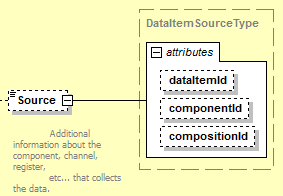
\includegraphics[width=.5\textwidth]{figures/source-schema-diagram.png}
  \caption{Source Diagram}
  \label{fig:source-schema-diagram}
\end{figure}
\FloatBarrier

\subparagraph{Attributes for Source} \mbox{}

\tbl{attributes-for-source} identifies the attributes available to identify \gls{source} for a measured value:

\tabulinesep = 5pt
\begin{longtabu} to \textwidth {
    |l|X[3l]|X[0.75l]|}
\caption{Attributes for Source} \label{table:attributes-for-source} \\

\hline
Attribute & Description & Occurrence \\
\hline
\endfirsthead

\hline
\multicolumn{3}{|c|}{Continuation of Table \ref{table:attributes-for-source}}\\
\hline
Attribute & Description & Occurrence \\
\hline
\endhead

\gls{componentid} 
&
\glsentrydesc{componentid}
\newline A \gls{valid data value} reported for \gls{componentid} \MUST be the value of the \gls{id} attribute for the \gls{component} element identified. \gls{componentid} is an optional attribute.
&
0..1 \DIFdelbegin \DIFdel{\notesign} \DIFdelend \\
\hline

\gls{dataitemid} 
&
\glsentrydesc{dataitemid}
\newline A \gls{valid data value} reported for \gls{dataitemid} \MUST be the value of the \gls{id} attribute for the \gls{dataitem} element identified.
\newline \gls{dataitemid} is an optional attribute.
&
0..1 \DIFdelbegin \DIFdel{\notesign} \DIFdelend \\
\hline

\gls{compositionid} 
&
The identifier attribute of the \gls{composition} element that represents the physical part of a piece of equipment where the data represented by the \gls{dataitem} element originated.
\newline A \gls{valid data value} reported for \gls{compositionid} \MUST be the value of the \gls{id} attribute for the \gls{composition} element identified.
\newline \gls{compositionid} is an optional attribute.
&
0..1 \DIFdelbegin \DIFdel{\notesign} \DIFdelend \\
\hline

\end{longtabu}




\DIFdelbegin %DIFDELCMD < \begin{note}
%DIFDELCMD < %%%
\DIFdel{Note: }%DIFDELCMD < \notesign %%%
\DIFdel{One of \gls{componentid}, \gls{compositionid}, or \gls{dataitemid} \must be provided.
}%DIFDELCMD < 

%DIFDELCMD < \end{note}
%DIFDELCMD < 

%DIFDELCMD < %%%
\DIFdelend

\paragraph{Constraints Element for DataItem}\mbox{}

For some types of \gls{dataitem} elements, the expected value(s) for the data reported for the \gls{dataitem} \may be restricted to specific values or a range of values.

\gls{constraints} is an optional XML element that provides a way to define the expected value(s) or the upper and lower limits for the range of values that are expected to be reported in response to a \gls{current request} or \gls{sample request}.

\gls{constraints} are used by a software application to evaluate the validity of the data reported.

The value associated with each \gls{constraint} element is reported in the \gls{cdata} for that element.

\subparagraph{Schema for Constraints} \mbox{}

The XML schema in \fig{constraints-schema-diagram} represents the structure of the \gls{constraints} XML element and the elements defined for \gls{constraints}.

\begin{figure}[ht]
  \centering
  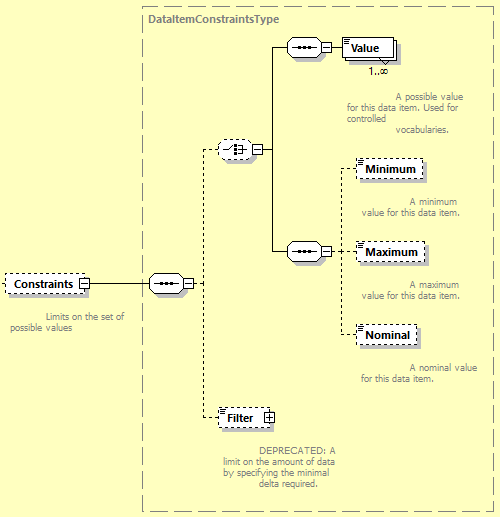
\includegraphics[width=.75\textwidth]{figures/constraints-schema-diagram.png}
  \caption{Constraints Diagram}
  \label{fig:constraints-schema-diagram}
\end{figure}
\FloatBarrier

\tbl{elements-for-constraints} identifies the elements available to identify \gls{constraints} for a measured value:

\tabulinesep = 5pt
\begin{longtabu} to \textwidth {
    |l|X[3l]|X[0.75l]|}
\caption{Elements for Constraints} \label{table:elements-for-constraints} \\

\hline
Element & Description & Occurrence \\
\hline
\endfirsthead

\hline
\multicolumn{3}{|c|}{Continuation of Table \ref{table:elements-for-constraints}}\\
\hline
Element & Description & Occurrence \\
\hline
\endhead

\gls{value}
&
\gls{value} represents a single data value that is expected to be reported for a \gls{dataitem} element.
\newline The data value is provided in the \gls{cdata} for this element and may be any numeric or text content.
\newline When there are multiple data values that may be expected to be reported for a \gls{dataitem} element, multiple \gls{value} elements may be defined.
\newline In the case where only one \gls{value} element is defined, the data returned in response to a \gls{current httprequest} or \gls{sample httprequest} request \MUST be the data value defined for \gls{value} element.
\newline \gls{value} \MUSTNOT be used in conjunction with any other \gls{constraint} elements.
&
0..* \\
\hline

\gls{maximum}
&
If the data reported for a data item is a range of numeric values, the expected value reported \MAY be described with an upper limit defined by this constraint.
\newline The data value is provided in the \gls{cdata} for this element and \MUST be a value using the same units as the reported data. 
&
0..1 \\
\hline

\gls{minimum}
&
If the data reported for a data item is a range of numeric values, the expected value reported \MAY be described with a lower limit defined by this constraint.
\newline The data value is provided in the \gls{cdata} for this element and \MUST be a value using the same units as the reported data. 
&
0..1 \\
\hline

\gls{nominal}
&
The target or expected value for this data item.
\newline The data value is provided in the \gls{cdata} for this element and \MUST be a value using the same units as the reported data. 
&
0..1 \\
\hline


\deprecated{\gls{filter}}
&
\DEPRECATED in Version 1.4 - Moved to the \gls{filters} element of a \gls{dataitem}.
\newline \deprecated{If the data reported for a DataItem is a numeric value, a new value MUST NOT be reported if the change from the last reported value is less than the delta given as the CDATA of this element. Filter is an abstract type XML element. As such, Filter will never appear in the XML document, but will be replaced by a Filter type. The only currently supported Filter type is MINIMUM_DELTA. The CDATA MUST be an absolute value using the same Units as the reported data. Additional filter types MAY be supported in the future.}
&
0..1 \notesign
\\ \hline

\end{longtabu}

\begin{note}
Note:	\notesign Remains in schema for backwards compatibility.
\end{note}

\paragraph{Filters Element for DataItem}\mbox{}

\gls{filters} is an optional XML container that organizes the \gls{filter} elements for \gls{dataitem}.

\gls{filters} contains one or more \gls{filter} XML elements.

\tabulinesep = 5pt
\begin{longtabu} to \textwidth {
    |l|X[3l]|X[0.75l]|}
\caption{MTConnect Filters Element} \label{table:mtconnect-filters-element} \\

\hline
Element & Description & Occurrence \\
\hline
\endfirsthead

\hline
\multicolumn{3}{|c|}{Continuation of Table \ref{table:mtconnect-filters-element}}\\
\hline
Element & Description & Occurrence \\
\hline
\endhead

\gls{filters}	
&
\glsentrydesc{filters}
 Only one \gls{filters} container \MAY appear for a \gls{dataitem} element.
&
0..1 \\
\hline


\end{longtabu}

\subparagraph{Filter} \mbox{}

\gls{filter} provides a means to control when an \gls{agent} records updated information for a data item.  Currently, there are two types of \gls{filter} elements defined in the MTConnect Standard - \gls{minimumdelta} and \gls{period}.   More \gls{filter} types may be added in the future.

The value associated with each \gls{filter} element is reported in the \gls{cdata} for that element.

\fig{filter-schema-diagram} represents the structure for \gls{filter} XML element.

\begin{figure}[ht]
  \centering
  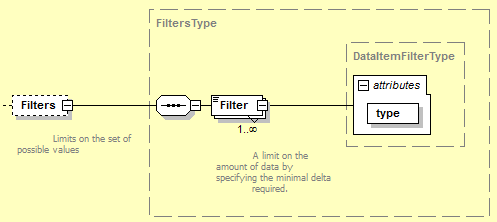
\includegraphics[width=.75\textwidth]{figures/filter-schema-diagram.png}
  \caption{Filter Diagram}
  \label{fig:filter-schema-diagram}
\end{figure}
\FloatBarrier

\tbl{dataitem-element-filter-type} describes the types of \gls{filter} defined for a \gls{dataitem} element and the expected behavior of an \gls{agent} when a \gls{filter} is applied to \gls{dataitem} element.

\tabulinesep = 5pt
\begin{longtabu} to \textwidth {
    |l|X[3l]|X[0.75l]|}
\caption{DataItem Element Filter type} \label{table:dataitem-element-filter-type} \\

\hline
type & Description & Occurrence \\
\hline
\endfirsthead

\hline
\multicolumn{3}{|c|}{Continuation of Table \ref{table:dataitem-element-filter-type}}\\
\hline
type & Description & Occurrence \\
\hline
\endhead

\gls{minimumdelta}
&
For a \gls{minimumdelta} type \gls{filter}, a new value \MUSTNOT be reported for a data item unless the measured value has changed from the last reported value by at least the delta given as the \gls{cdata} of this element.
\newline The \gls{cdata} \MUST be an absolute value using the same units as the reported data. 
&
0..1 \notesign \\
\hline

\gls{period}
&
For a \gls{period} type \gls{filter}, the data reported for a data item is provided on a periodic basis. The \gls{period} for reporting data is defined in the \gls{cdata} for the \gls{filter}.
\newline The \gls{cdata} \MUST be an absolute value reported in seconds representing the time between reported samples of the value of the data item.
\newline If the \gls{period} is smaller than one second, the number can be represented as a floating point number. For example, a \gls{period} of 100 milliseconds would be 0.1.
&
0..1 \notesign \\
\hline

\end{longtabu}

\begin{note}
	Note:	\notesign Either \gls{minimumdelta} or \gls{period} can be defined, not both.
\end{note}

\paragraph{InitialValue Element for DataItem}\mbox{}

\gls{initialvalue} is an XML element that defines the value to be set for the data item after a reset event.

The value associated with the \gls{initialvalue} element is reported in the \gls{cdata} for this element and \must be an absolute value using the same units as the reported data.

\paragraph{ResetTrigger Element for DataItem}\mbox{}

The value of some data types is periodically reset to the value of the \gls{initialvalue} element.   These reset events may be based upon a specific elapsed time or may be triggered by a physical or logical reset action that causes the reset to occur.   \gls{resettrigger} provides additional information regarding the meaning of the data - establishing an understanding of the time frame that the data represents so that the data may be correctly understood by a client software application.

\tabulinesep = 5pt
\begin{longtabu} to \textwidth {
    |l|X[3l]|X[0.75l]|}
\caption{MTConnect ResetTrigger Element} \label{table:mtconnect-resettrigger-element} \\

\hline
Element & Description & Occurrence \\
\hline
\endfirsthead

\hline
\multicolumn{3}{|c|}{Continuation of Table \ref{table:mtconnect-resettrigger-element}}\\
\hline
Element & Description & Occurrence \\
\hline
\endhead

\gls{resettrigger}
&
\gls{resettrigger} is an XML element that describes the reset action that causes a reset to occur.
\newline It is additional information regarding the meaning of the data that establishes an understanding of the time frame that the data represents so that the data may be correctly understood by a client software application.
&
0..1 \\
\hline


\end{longtabu}


The reset action that \may cause a reset to occur is provided in the \gls{cdata} for this element. 

The reset actions that may cause a reset to occur are described in \tbl{dataitem-element-resettrigger-type}.

\tabulinesep = 5pt
\begin{longtabu} to \textwidth {
    |l|X[3l]|}
\caption{DataItem Element ResetTrigger type} \label{table:dataitem-element-resettrigger-type} \\

\hline
Reset Actions & Description\\
\hline
\endfirsthead

\hline
\multicolumn{2}{|c|}{Continuation of Table \ref{table:dataitem-element-resettrigger-type}} \\
\hline
Reset Actions & Description\\
\hline
\endhead

\gls{actioncomplete} & 
The value of the \gls{data entity} that is measuring an action or
operation is to be reset upon completion of that action or
operation. \\ \hline 

\gls{annual} & 
The value of the \gls{data entity} is to be reset at the end of a 12-month period.\\ \hline 

\gls{day} & 
The value of the \gls{data entity} is to be reset at the end of a 24-hour
period.\\ \hline 

\gls{life} & 
The value of the \gls{data entity} is not reset and accumulates for the
entire life of the piece of equipment.\\ \hline 

\gls{maintenance}
& 
The value of the \gls{data entity} is to be reset upon completion of a maintenance event.
\\ \hline 

\gls{month} & 
The value of the \gls{data entity} is to be reset at the end of a monthly
period. \\ \hline 

\gls{poweron} & 
The value of the \gls{data entity} is to be reset when power was
applied to the piece of equipment after a planned or unplanned
interruption of power has occurred.\\ \hline 

\gls{shift} & 
The value of the \gls{data entity} is to be reset at the end of a work
shift.\\ \hline 

\gls{week} & 
The value of the \gls{data entity} is to be reset at the end of a 7-day
period.\\ \hline 



\end{longtabu}


\section{Listing of Data Items}
\label{sec:Listing of Data Items}

In the MTConnect Standard, \gls{dataitem} elements are defined and organized based upon the \gls{category} and \gls{type} attributes.  
The \gls{category} attribute provides a high level grouping for \gls{dataitem} elements based on the kind of information that is reported by the data item.

These categories are:

\begin{itemize}

\item \gls{sample category}

A \gls{sample category} reports a continuously variable or analog data value. 

\item \gls{event category}

An \gls{event category} reports information representing a functional state, with two or more discrete values, associated with a component or it contains a message.  The data provided may be a numeric value or text.

\item \gls{condition category}

A \gls{condition category} reports information about the health of a piece of equipment and its ability to function.
\end{itemize}

The \gls{type} attribute specifies the specific kind of data that is reported.   For some types of data items, a \gls{subtype} attribute may also be used to differentiate between multiple data items of the same \gls{type} where the information reported by the data item has a different, but related, meaning.

Many types of data items provide two forms of data: a value (reported as either a \gls{sample category} or \gls{event category}) and a health status (reported as a \gls{condition category}).  These \gls{dataitem} types \may be defined in more than one \gls{category} based on the data that they report.

\subsection{Data Items in category SAMPLE}

The types of \gls{dataitem} elements in the \gls{sample category} category report data representing a continuously changing or analog data value.  This data can be measured at any point-in-time and will always produce a result.  The data provided may be a scalar floating point number or integers that have an infinite number of possible values.  The \gls{units} attribute \must be defined and reported for each \gls{dataitem} in this category.

\tbl{dataitem-type-category-sample} defines the types and subtypes of \gls{dataitem} elements defined for the \gls{sample category} category.  The subtypes are indented below their associated types. 

\tabulinesep = 5pt
\begin{longtabu} to \textwidth {
    |X[3l]|X[3l]|X[2.8l]|}
\caption{DataItem type subType for category SAMPLE} \label{table:dataitem-type-category-sample} \\

\hline
DataItem type/subType & Description & Units\\
\hline
\endfirsthead

\hline
\multicolumn{3}{|c|}{Continuation of Table \ref{table:dataitem-type-category-sample}}\\
\hline
DataItem type/subType & Description & Units\\
\hline
\endhead

\gls{acceleration sample}
&
Rate of change of velocity.
&
\glsentryunits{acceleration sample} \\ \hline 

\gls{accumulatedtime sample} 
& 
\glsentrydesc{accumulatedtime sample} 
\newline \DEPRECATIONWARNING:  May be deprecated in the future.  Recommend using \gls{processtimer sample} and \gls{equipmenttimer sample}.
& 
\glsentryunits{accumulatedtime sample} \\ \hline 

\gls{amperage sample} & \glsentrydesc{amperage sample} & \glsentryunits{amperage sample} \\ \hline 

\quad \gls{actual subtype}
&
The measured amperage being delivered from a power source.
&
\glsentryunits{amperage sample} \\ \hline 

\quad \gls{alternating subtype}
& 
The measurement of alternating current.   If not specified further in \gls{statistic}, defaults to RMS voltage.
& \glsentryunits{amperage sample} \\ \hline 

\quad \gls{direct subtype}
&
The measurement of DC current.
& \glsentryunits{amperage sample} \\ \hline 

\quad \gls{target subtype}
&
The desired or preset amperage to be delivered from a power source.
& \glsentryunits{amperage sample} \\ \hline 

\gls{angle sample} & \glsentrydesc{angle sample} & \glsentryunits{angle sample} \\ \hline 

\quad \gls{actual subtype}
&
The actual angular position as read from the physical component.
&
\glsentryunits{angle sample} \\ \hline 

\quad \gls{commanded subtype}
&
A calculated value for angular position computed by the \gls{controller} type component.
& \glsentryunits{angle sample} \\ \hline 

\gls{angularacceleration sample}
&
Rate of change of angular velocity. 
& \glsentryunits{angularacceleration sample} \\ \hline 

\gls{angularvelocity sample}
& 
Rate of change of angular position.
& \glsentryunits{angularvelocity sample} \\ \hline 

\gls{axisfeedrate sample}
&
The feedrate of a linear axis.
& \glsentryunits{axisfeedrate sample} \\ \hline 

\quad \gls{actual subtype}
&
The measured value of the feedrate of a linear axis.
&
\glsentryunits{axisfeedrate sample} \\ \hline 

\quad \gls{commanded subtype}
&
The feedrate of a linear axis as specified by the \gls{controller} type component.
\newline The \gls{commanded subtype} feedrate is a calculated value that includes adjustments and overrides.
& \glsentryunits{axisfeedrate sample} \\ \hline 

\quad \gls{jog subtype}
&
The feedrate specified by a logic or motion program, by a pre-set value, or set by a switch as the feedrate for a linear axis when operating in a manual state or method (jogging).  
& \glsentryunits{axisfeedrate sample} \\ \hline 

\quad \deprecated{\gls{override subtype}}
&
\deprecated{The operator's overridden value. Percent of commanded.} \DEPRECATED in Version 1.3. See \gls{event category} category data items.
& \deprecated{\gls{percent}} \\ \hline 

\quad \gls{programmed subtype}
&
The feedrate specified by a logic or motion program or set by a switch for a linear axis.
& \glsentryunits{axisfeedrate sample} \\ \hline 

\quad \gls{rapid subtype}
&
The feedrate specified by a logic or motion program, by a pre-set value, or set by a switch as the feedrate for a linear axis when operating in a rapid positioning mode.
& \glsentryunits{axisfeedrate sample} \\ \hline 

\gls{clocktime sample} 
& 
\glsentrydesc{clocktime sample} 
\newline \gls{clocktime sample} \must be reported in W3C ISO 8601 format.
& 
\glsentryunits{clocktime sample} \\ \hline 

\gls{concentration sample} &
Percentage of one component within a mixture of components.
& \glsentryunits{concentration sample} \\ \hline 

\gls{conductivity sample} & 
The ability of a material to conduct electricity.
& \glsentryunits{conductivity sample} \\ \hline 

\gls{displacement sample} & 
The change in position of an object.
& \glsentryunits{displacement sample} \\ \hline 

\gls{electricalenergy sample} & \glsentrydesc{electricalenergy sample} & \glsentryunits{electricalenergy sample} \\ \hline 

\gls{equipmenttimer sample} 
& 
\glsentrydesc{equipmenttimer sample} 
  Often used to determine when maintenance may be required for the equipment. 
\newline Multiple \glspl{subtype} of \gls{equipmenttimer sample} \MAY be defined. 
\newline A \gls{subtype} \must always be specified.
& 
\glsentryunits{equipmenttimer sample} 
\\ \hline 

\quad \gls{delay subtype}
&
Measurement of the time that a piece of equipment is waiting for an event or an action to occur.
& \glsentryunits{equipmenttimer sample} \\ \hline 

\quad \gls{loaded subtype}
&
Measurement of the time that the sub-parts of a piece of equipment are under load. \newline Example: For traditional machine tools, this is a measurement of the time that the cutting tool is assumed to be engaged with the part.
& \glsentryunits{equipmenttimer sample} \\ \hline 

\quad \gls{operating subtype}
&
Measurement of the time that the major sub-parts of a piece of equipment are powered or performing any activity whether producing a part or product or not.   \newline Example: For traditional machine tools, this includes \gls{working subtype}, plus idle time.
& \glsentryunits{equipmenttimer sample} \\ \hline 

\quad \gls{powered subtype}
&
The measurement of time that primary power is applied to the piece of equipment and, as a minimum, the controller or logic portion of the piece of equipment is powered and functioning or components that are required to remain on are powered. 
\newline Example: Heaters for an extrusion machine that are required to be powered even when the equipment is turned off
& \glsentryunits{equipmenttimer sample} \\ \hline 

\quad \gls{working subtype}
&
Measurement of the time that a piece of equipment is performing any activity  the equipment is active and performing a function under load or not. \newline Example: For traditional machine tools, this includes \gls{loaded subtype}, plus rapid moves, tool changes, etc.
& \glsentryunits{equipmenttimer sample} \\ \hline 

\gls{filllevel sample} & \glsentrydesc{filllevel sample} & \glsentryunits{filllevel sample} \\ \hline 

\gls{flow sample} &
The rate of flow of a fluid.
& \glsentryunits{flow sample} \\ \hline 

\gls{frequency sample} & \glsentrydesc{frequency sample} & \glsentryunits{frequency sample} \\ \hline 

\gls{globalposition sample} & \glsentrydesc{globalposition sample} & \glsentryunits{globalposition sample} \\ \hline 

\gls{length sample} &
The length of an object.
& \glsentryunits{length sample} \\ \hline 

\quad \gls{remaining subtype}
&
The remaining total length of an object.
& \glsentryunits{length sample} \\ \hline 

\quad \gls{standard subtype} & \glsentrydesc{standard subtype} & \glsentryunits{standard subtype} \\ \hline 

\quad \gls{useable subtype} & \glsentrydesc{useable subtype} & \glsentryunits{useable subtype} \\ \hline 

\gls{level sample} & \glsentrydesc{level sample} & \glsentryunits{level sample} \\ \hline 

\gls{linearforce sample} & \glsentrydesc{linearforce sample} & \glsentryunits{linearforce sample} \\ \hline 

\gls{load sample} & \glsentrydesc{load sample} & \glsentryunits{load sample} \\ \hline 

\gls{mass sample} & \glsentrydesc{mass sample} & \glsentryunits{mass sample} \\ \hline 

\gls{pathfeedrate sample}
&
The feedrate for the axes, or a single axis, associated with a \gls{path} component- a vector. 
& \glsentryunits{pathfeedrate sample} \\ \hline 

\quad \gls{actual subtype} 
&
The measured value of the feedrate of the axes, or a single axis, associated with a path component.
&
\glsentryunits{pathfeedrate sample} \\ \hline 

\quad \gls{commanded subtype} 
&
The feedrate as specified by the \gls{controller} type component for the axes, or a single axis, associated with a \gls{path} component.
\newline The \gls{commanded subtype} feedrate is a calculated value that includes adjustments and overrides.
& \glsentryunits{pathfeedrate sample} \\ \hline 

\quad \gls{jog subtype}
&
The feedrate specified by a logic or motion program, by a pre-set value, or set by a switch as the feedrate for the axes, or a single axis, associated with a \gls{path} when operating in a manual state or method (jogging).
& \glsentryunits{pathfeedrate sample} \\ \hline 

\quad \deprecated{\gls{override subtype}}
&
\deprecated{The operator's overridden value. Percent of commanded.} \DEPRECATED in Version 1.3. See \gls{event category} category data items.
& \deprecated{\gls{percent}} \\ \hline 

\quad \gls{programmed subtype}
&
The feedrate specified by a logic or motion program or set by a switch as the feedrate for the axes, or a single axis, associated with a \gls{path}.
& \glsentryunits{pathfeedrate sample} \\ \hline 

\quad \gls{rapid subtype}
&
The feedrate specified by a logic or motion program, by a pre-set value, or set by a switch as the feedrate for the axes, or a single axis, associated with a \gls{path} when operating in a rapid positioning mode.
& \glsentryunits{pathfeedrate sample} \\ \hline

\gls{pathposition sample}
&
\DIFdelbegin \DIFdel{\glsentrydesc{pathposition sample} 
}%DIFDELCMD < \newline %%%
\DIFdelend \DIFaddbegin \DIFadd{A measured or calculated position of a control point associated with a piece of equipment. }\DIFaddend The control point \MUST be reported as a set of space-delimited floating-point numbers representing a point in 3-D space. The position of the control point \MUST be reported in units of \gls{millimeter} and listed in order of X, Y, and Z referenced to the coordinate system of the piece of equipment. Any control point representing a position in 1-D or 2-D space \MAY be represented in terms of 3-D space by setting any undefined coordinate to zero (0). \DIFdelbegin %DIFDELCMD < \newline %%%
\DIFdel{\gls{pathposition sample} \should }\DIFdelend \DIFaddbegin \DIFadd{\gls{pathposition sample} \SHOULD }\DIFaddend be further defined with a \gls{coordinatesystem} attribute. If a \gls{coordinatesystem} attribute is not specified, the position of the control point \MUST be reported in \gls{work} coordinates.
&
\glsentryunits{pathposition sample} \\
\hline

\quad \gls{actual subtype}
&
The measured position of the current program control point as reported by the piece of equipment.
&
\glsentryunits{pathposition sample} \\
\hline

\quad \DIFadd{\gls{programmed subtype}
}&
\DIFadd{The position of the control point specified by a logic or motion program
}&
\DIFadd{\glsentryunits{pathposition sample} }\\
\hline

\quad \gls{commanded subtype}
&
The position computed by the \gls{controller} type component.
&
\glsentryunits{pathposition sample} \\
\hline

\quad \gls{probe subtype}
&
The position provided by a measurement probe. &
\glsentryunits{pathposition sample} \\
\hline

\quad \gls{target subtype}
&
The desired end position for a movement or a series of movements. \DIFdelbegin %DIFDELCMD < \newline %%%
\DIFdelend Multiple discrete movements may need to be completed to achieve the final \gls{target subtype} position.
&
\glsentryunits{pathposition sample} \\
\hline 

\gls{ph sample} 
&
The measurement of the acidity or alkalinity.
& \glsentryunits{ph sample} \\ \hline 

\gls{position sample}
& 
\glsentrydesc{position sample} 
\newline \gls{position sample} \should be further defined with a coordinateSytem attribute.  If a \gls{coordinatesystem} attribute is not specified, the position of the control point \must be reported in \gls{machine} coordinates.
& 
\glsentryunits{position sample} \\ \hline 

\quad \gls{actual subtype}
&
The physical measured position of the control point for a \gls{component}. 
&
\glsentryunits{position sample} \\ \hline 

\quad \gls{commanded subtype}
&
A position calculated by the \gls{controller} type component for a discrete movement.
& \glsentryunits{position sample} \\ \hline 

\quad \gls{programmed subtype}
&
The position of the control point for a \gls{component} specified by a logic or motion program.
& \glsentryunits{position sample} \\ \hline 

\quad \gls{target subtype}
&
The desired end position of the control point for a \gls{component} resulting from a movement or a series of movements.  
\newline Multiple discrete movements may need to be completed to achieve the final \gls{target subtype} position.
& \glsentryunits{position sample} \\ \hline 

\gls{powerfactor sample} & \glsentrydesc{powerfactor sample} & \glsentryunits{powerfactor sample} \\ \hline 

\gls{pressure sample} & 
The force per unit area exerted by a gas or liquid.
& \glsentryunits{pressure sample} \\ \hline 

\gls{processtimer sample} 
& 
\glsentrydesc{processtimer sample} 
\newline Multiple subtypes of \gls{processtimer sample} may be defined. 
\newline Typically, \gls{processtimer sample} \should be modeled as a data item for the Device element, but \MAY be modeled for either a \gls{controller} or \gls{path} \gls{structural element} in the XML document.
\newline A \gls{subtype} \must always be specified.
& 
\glsentryunits{processtimer sample} \\ \hline 

\quad \gls{delay subtype}
&
Measurement of the time that a process is waiting and unable to perform its intended function.
& \glsentryunits{processtimer sample} \\ \hline

\quad \gls{process processtimer sample} & \glsentrydesc{process processtimer sample} & \glsentryunits{process processtimer sample} \\ \hline 

\gls{resistance sample} &
The degree to which a substance opposes the passage of an electric current. 
& \glsentryunits{resistance sample} \\ \hline 

\gls{rotaryvelocity sample} &
The rotational speed of a rotary axis.
& \glsentryunits{rotaryvelocity sample} \\ \hline 

\quad \gls{actual subtype}
&
The measured value of rotational speed that the rotary axis is spinning.
&
\glsentryunits{rotaryvelocity sample} \\ \hline 

\quad \gls{commanded subtype}
&
The rotational speed as specified by the \gls{controller} type component.
\newline The \gls{commanded subtype} velocity is a calculated value that includes adjustments and overrides.
& \glsentryunits{rotaryvelocity sample} \\ \hline 

\quad \deprecated{\gls{override subtype}}
&
\deprecated{The operator's overridden value. Percent of commanded.} \DEPRECATED in Version 1.3. See \gls{event category} category data items.
& \deprecated{\gls{percent}} \\ \hline 

\quad \gls{programmed subtype}
&
The rotational velocity specified by a logic or motion program or set by a switch.
& \glsentryunits{rotaryvelocity sample} \\ \hline 

\gls{soundlevel sample} & \glsentrydesc{soundlevel sample} & \glsentryunits{soundlevel sample} \\ \hline 

\quad \gls{ascale subtype} & \glsentrydesc{ascale subtype} & \glsentryunits{soundlevel sample} \\ \hline 

\quad \gls{bscale subtype} & \glsentrydesc{bscale subtype} & \glsentryunits{soundlevel sample} \\ \hline 

\quad \gls{cscale subtype} & \glsentrydesc{cscale subtype} & \glsentryunits{soundlevel sample} \\ \hline 

\quad \gls{dscale subtype} & \glsentrydesc{dscale subtype} & \glsentryunits{soundlevel sample} \\ \hline 

\quad \gls{noscale subtype} & \glsentrydesc{noscale subtype} & \glsentryunits{soundlevel sample} \\ \hline 

\gls{spindlespeed sample} & \glsentrydesc{spindlespeed sample} & \deprecated{\glsentryunits{spindlespeed sample}} \\ \hline 

\quad \deprecated{\gls{actual subtype}}
&
\deprecated{The rotational speed of a rotary axis.\newline  \gls{rotarymode event} \must be \gls{spindle value}.}
&
\deprecated{\glsentryunits{spindlespeed sample}} \\ \hline 

\quad \deprecated{\gls{commanded subtype}}
&
\deprecated{The rotational speed the as specified by the \gls{controller} type \gls{component}.}
&
\deprecated{\glsentryunits{spindlespeed sample}} \\ \hline 

\quad \deprecated{\gls{override subtype}}
&
\deprecated{The operator's overridden value. Percent of commanded.}
&
\deprecated{\gls{percent}} \\ \hline 

\gls{strain sample} &
The amount of deformation per unit length of an object when a load is applied. 
& \glsentryunits{strain sample} \\ \hline 

\gls{temperature sample} & \glsentrydesc{temperature sample} & \glsentryunits{temperature sample} \\ \hline 

\gls{tension sample} & \glsentrydesc{tension sample} & \glsentryunits{tension sample} \\ \hline 

\gls{tilt sample} & \glsentrydesc{tilt sample} & \glsentryunits{tilt sample} \\ \hline 

\gls{torque sample} & 
The turning force exerted on an object or by an object.
& \glsentryunits{torque sample} \\ \hline 

\gls{velocity sample} &
The rate of change of position.
& \glsentryunits{velocity sample} \\ \hline 

\gls{viscosity sample} & \glsentrydesc{viscosity sample} & \glsentryunits{viscosity sample} \\ \hline 

\gls{voltampere sample} & \glsentrydesc{voltampere sample} & \glsentryunits{voltampere sample} \\ \hline 

\gls{voltamperereactive sample} & \glsentrydesc{voltamperereactive sample} & \glsentryunits{voltamperereactive sample} \\ \hline 

\gls{voltage sample} & \glsentrydesc{voltage sample} & \glsentryunits{voltage sample} \\ \hline 

\quad \gls{actual subtype}
&
The measured voltage being delivered from a power source.
&
\glsentryunits{voltage sample} \\ \hline 

\quad \gls{alternating subtype}
& 
The measurement of alternating voltage.   If not specified further in statistic, defaults to RMS voltage.
& \glsentryunits{voltage sample} \\ \hline 

\quad \gls{direct subtype}
&
The measurement of DC voltage.
& \glsentryunits{voltage sample} \\ \hline 

\quad \gls{target subtype}
&
The desired or preset voltage to be delivered from a power source.
& \glsentryunits{voltage sample} \\ \hline 

\gls{wattage sample} & \glsentrydesc{wattage sample} & \glsentryunits{wattage sample} \\ \hline 

\quad \gls{actual subtype}
&
The measured wattage being delivered from a power source.
&
\glsentryunits{wattage sample} \\ \hline 

\quad \gls{target subtype}
&
The desired or preset wattage to be delivered from a power source.
& \glsentryunits{wattage sample} \\ \hline 





\DIFaddbegin \DIFadd{\gls{volumespatial sample}
}&
\DIFadd{The geometric volume of an object or container.
}&
\DIFadd{\glsentryunits{volumespatial sample} }\\
\hline

\quad \DIFadd{\gls{actual subtype}
}&
\DIFadd{The amount of bulk material currently present in an object or container.
}&
\DIFadd{\glsentryunits{volumespatial sample} }\\
\hline

\quad \DIFadd{\gls{consumed subtype}
}&
\DIFadd{The amount of bulk material consumed from an object or container during a manufacturing process.
}&
\DIFadd{\glsentryunits{volumespatial sample} }\\
\hline

\DIFadd{\gls{volumefluid sample}
}&
\DIFadd{The fluid volume of an object or container.
}&
\DIFadd{\glsentryunits{volumefluid sample} }\\
\hline

\quad \DIFadd{\gls{actual subtype}
}&
\DIFadd{The amount of fluid currently present in an object or container.
}&
\DIFadd{\glsentryunits{volumefluid sample} }\\
\hline

\quad \DIFadd{\gls{consumed subtype}
}&
\DIFadd{The amount of fluid material consumed from an object or container during a manufacturing process.
}&
\DIFadd{\glsentryunits{volumefluid sample} }\\
\hline

\DIFadd{\gls{capacityspatial sample}
}&
\DIFadd{The geometric capacity of an object or container.
}&
\DIFadd{\glsentryunits{capacityspatial sample} }\\
\hline

\DIFadd{\gls{capacityfluid sample}
}&
\DIFadd{The fluid capacity of an object or container.
}&
\DIFadd{\glsentryunits{capacityfluid sample} }\\
\hline

\DIFadd{\gls{density sample}
}&
\DIFadd{The volumetric mass of a material per unit volume of that material.
}&
\DIFadd{\glsentryunits{density sample} }\\
\hline

\DIFadd{\gls{depositionvolume sample}
}&
\DIFadd{The spatial volume of material to be deposited in an additive manufacturing process.
}&
\DIFadd{\glsentryunits{depositionvolume sample} }\\
\hline

\quad \DIFadd{\gls{actual subtype}
}&
\DIFadd{The measured spatial volume of material deposited.
}&
\DIFadd{\glsentryunits{depositionvolume sample} }\\
\hline

\quad \DIFadd{\gls{commanded subtype}
}&
\DIFadd{The target spatial volume of material to be deposited.
}&
\DIFadd{\glsentryunits{depositionvolume sample} }\\
\hline

\DIFadd{\gls{depositionratevolumetric sample}
}&
\DIFadd{The rate at which a spatial volume of material is deposited in an additive manufacturing process.
}&
\DIFadd{\glsentryunits{depositionratevolumetric sample} }\\
\hline

\quad \DIFadd{\gls{actual subtype}
}&
\DIFadd{The measured rate at which a spatial volume of material is deposited in an additive manufacturing process.
}&
\DIFadd{\glsentryunits{depositionratevolumetric sample} }\\
\hline

\quad \DIFadd{\gls{commanded subtype}
}&
\DIFadd{The programmed rate at which a spatial volume of material is to be deposited in an additive manufacturing process.
}&
\DIFadd{\glsentryunits{depositionratevolumetric sample} }\\
\hline

\DIFadd{\gls{depositionaccelerationvolumetric sample}
}&
\DIFadd{The rate of change in spatial volume of material deposited in an additive manufacturing process.
}&
\DIFadd{\glsentryunits{depositionaccelerationvolumetric sample} }\\
\hline

\quad \DIFadd{\gls{actual subtype}
}&
\DIFadd{The measured rate of change in spatial volume of material deposited in an additive manufacturing process.
}&
\DIFadd{\glsentryunits{depositionaccelerationvolumetric sample} }\\
\hline

\quad \DIFadd{\gls{commanded subtype}
}&
\DIFadd{The commanded rate of change in spatial volume of material to be deposited in an additive manufacturing process.
}&
\DIFadd{\glsentryunits{depositionaccelerationvolumetric sample} }\\
\hline

\DIFadd{\gls{depositionmass sample}
}&
\DIFadd{The mass of the material deposited in an additive manufacturing process.
}&
\DIFadd{\glsentryunits{depositionmass sample} }\\
\hline

\quad \DIFadd{\gls{actual subtype}
}&
\DIFadd{The measured mass of the material deposited in an additive manufacturing process.
}&
\DIFadd{\glsentryunits{depositionmass sample} }\\
\hline

\quad \DIFadd{\gls{commanded subtype}
}&
\DIFadd{The commanded mass of the material to be deposited in an additive manufacturing process.
}&
\DIFadd{\glsentryunits{depositionmass sample} }\\
\hline

\DIFadd{\gls{depositiondensity sample}
}&
\DIFadd{The density of the material deposited in an additive manufacturing process per unit of volume.
}&
\DIFadd{\glsentryunits{depositiondensity sample} }\\
\hline

\quad \DIFadd{\gls{actual subtype}
}&
\DIFadd{The measured density of the material deposited in an additive manufacturing process.
}&
\DIFadd{\glsentryunits{depositiondensity sample} }\\
\hline

\quad \DIFadd{\gls{commanded subtype}
}&
\DIFadd{The commanded density of material to be deposited in an additive manufacturing process.
}&
\DIFadd{\glsentryunits{depositiondensity sample} }\\
\hline

\DIFadd{\gls{cuttingspeed sample}
}&
 \DIFadd{The speed difference (relative velocity) between the cutting mechanism and the surface of the workpiece it is operating on.
}&
\DIFadd{\glsentryunits{cuttingspeed sample} }\\
\hline

\quad \DIFadd{\gls{actual subtype}
}&
\DIFadd{The measured value between the cutting mechanism and the surface of the workpiece it is operating on.
}&
\DIFadd{\glsentryunits{cuttingspeed sample} }\\
\hline

\quad \DIFadd{\gls{commanded subtype}
}&
\DIFadd{The commanded value between the cutting mechanism and the surface of the workpiece it is operating on.
}&
\DIFadd{\glsentryunits{cuttingspeed sample} }\\
\hline

\quad \DIFadd{\gls{programmed subtype}
}&
\DIFadd{The programmed value between the cutting mechanism and the surface of the workpiece it is operating on.
}&
\DIFadd{\glsentryunits{cuttingspeed sample} }\\
\hline

\DIFadd{\gls{pathfeedrateperrevolution sample}
}&
\DIFadd{The feedrate for the axes, or a single axis.
}&
\DIFadd{\glsentryunits{pathfeedrateperrevolution sample} }\\
\hline

\quad \DIFadd{\gls{actual subtype}
}&
\DIFadd{The measured value of the feedrate of the axes, or a single axis.
}&
\DIFadd{\glsentryunits{pathfeedrateperrevolution sample} }\\
\hline

\quad \DIFadd{\gls{commanded subtype}
}&
\DIFadd{The feedrate as specified by the \gls{controller} for the axes, or a single axis. The \gls{commanded subtype} feedrate is a calculated value that includes adjustments and overrides.
}&
\DIFadd{\glsentryunits{pathfeedrateperrevolution sample} }\\
\hline

\quad \DIFadd{\gls{programmed subtype}
}&
\DIFadd{The feedrate specified by a logic or motion program or set by a switch as the feedrate for the axes, or a single axis.
}&
\DIFadd{\glsentryunits{pathfeedrateperrevolution sample} }\\
\hline\DIFaddend \end{longtabu}

\subsection{Data Items in category EVENT}

\gls{dataitem} types in the \gls{event category} category represent a discrete piece of information from a piece of equipment.  \gls{event category} does not have intermediate values that vary over time.

An \gls{event category} is information that, when provided at any specific point in time, represents the current state of the piece of equipment.

There are two types of \gls{event category}: those representing state, with two or more discrete values, and those representing messages that contain plain text data.

\tbl{dataitem-type-category-event} defines the \gls{dataitem} types and subtypes defined for the \gls{event category} category.  The subtypes are indented below their associated types. 

\tabulinesep = 5pt
\begin{longtabu} to \textwidth {
    |l|X[3l]|}
\caption{DataItem type subType for category EVENT} \label{table:dataitem-type-category-event} \\

\hline
DataItem type subType & Description\\
\hline
\endfirsthead

\hline
\multicolumn{2}{|c|}{Continuation of Table \ref{table:dataitem-type-category-event}}\\
\hline
DataItem type subType & Description\\
\hline
\endhead

\gls{activeaxes event} &
\glsentrydesc{activeaxes event}
\newline If this \gls{dataitem} is not provided, it will be assumed that all axes are currently associated with the \gls{controller} \gls{structural element} and with an individual \gls{path}.   
\newline The \gls{valid data value} for \gls{activeaxes event} \should be a space-delimited set of axes reported as the value of the \gls{name} attribute for each axis.  If \gls{name} is not available, the piece of equipment \must report the value of the \gls{nativename} attribute for each axis.
\\ \hline 

\gls{actuatorstate event} &
\glsentrydesc{actuatorstate event}
\newline The \gls{valid data value} \must be \gls{active value} or \gls{inactive value}.
\\ \hline 

\gls{alarm event}
&
\DEPRECATED in Version 1.1. Replaced with \gls{condition category} category.
\\ \hline 

\gls{availability event}
&
\glsentrydesc{availability event}
\newline This \must be provided for a \gls{device} Element and \MAY be provided for any other \gls{structural element}.  The \gls{valid data value} \must be \gls{available value} or \gls{unavailable value}.\\ \hline 

\gls{axiscoupling event} &
\glsentrydesc{axiscoupling event} 
\newline The \gls{valid data value} \must be \gls{tandem value}, \gls{synchronous value}, \gls{master value}, and \gls{slave value}.  
\newline The coupling \must be viewed from the perspective of a specific axis.  Therefore, a \gls{master value} coupling indicates that this axis is the master for the \gls{coupledaxes event}.
\\ \hline 

\gls{axisfeedrateoverride event} & \glsentrydesc{axisfeedrateoverride event}
\newline The value provided for \gls{axisfeedrateoverride event} is expressed as a percentage of the designated feedrate for the axis.   
\newline When \gls{axisfeedrateoverride event} is applied, the resulting commanded feedrate for the axis is limited to the value of the original feedrate multiplied by the value of the \gls{axisfeedrateoverride event}.   
\newline There \MAY be different subtypes of \gls{axisfeedrateoverride event}; each representing an override value for a designated subtype of feedrate depending on the state of operation of the axis.   The subtypes of operation of an axis are currently defined as \gls{programmed subtype}, \gls{jog subtype}, and \gls{rapid subtype}.
\\ \hline 

\quad \gls{jog subtype}
&
The value of a signal or calculation issued to adjust the feedrate of an individual linear type axis when that axis is being operated in a manual state or method (jogging).   \newline When the \gls{jog subtype} subtype of \gls{axisfeedrateoverride event} is applied, the resulting commanded feedrate for the axis is limited to the value of the original \gls{jog subtype} subtype of the \gls{axisfeedrate sample} multiplied by the value of the \gls{jog subtype} subtype of \gls{axisfeedrateoverride event}.
\\ \hline 

\quad \gls{programmed subtype}
&
The value of a signal or calculation issued to adjust the feedrate of an individual linear type axis that has been specified by a logic or motion program or set by a switch. \newline When the \gls{programmed subtype} subtype of \gls{axisfeedrateoverride event} is applied, the resulting commanded feedrate for the axis is limited to the value of the original \gls{programmed subtype} subtype of the \gls{axisfeedrate sample} multiplied by the value of the \gls{programmed subtype} subtype of \gls{axisfeedrateoverride event}. \\ \hline 

\quad \gls{rapid subtype}
&
The value of a signal or calculation issued to adjust the feedrate of an individual linear type axis that is operating in a rapid positioning mode. 
\newline When the \gls{rapid subtype} subtype of \gls{axisfeedrateoverride event} is applied, the resulting commanded feedrate for the axis is limited to the value of the original \gls{rapid subtype} subtype of the \gls{axisfeedrate sample} multiplied by the value of the \gls{rapid subtype} subtype of \gls{axisfeedrateoverride event}. \\ \hline 

\gls{axisinterlock event} 
& 
\glsentrydesc{axisinterlock event} 
\newline The \gls{valid data value} \must be \gls{active value} or \gls{inactive value}.
\\ \hline 

\gls{axisstate event} 
& 
\glsentrydesc{axisstate event}
\newline The \gls{valid data value} \must be \gls{home value}, \gls{travel value}, \gls{parked value}, or \gls{stopped value}.
\\ \hline 

\gls{block event}
& 
\glsentrydesc{block event} 
\newline The value reported for \glselementname{block event} \must include the entire expression for a line of program code, including all parameters.
\\ \hline 

\gls{blockcount event} 
& 
\glsentrydesc{blockcount event} 
\newline \gls{blockcount event} counts blocks of program code executed regardless of program structure (e.g., looping or branching within the program).
\newline The starting value for \gls{blockcount event} \MAY be established by an initial value provided in the Constraint element defined for the data item.
\\ \hline 

\gls{chuckinterlock event} 
& 
\glsentrydesc{chuckinterlock event} 
\newline The \gls{valid data value} \must be \gls{active value} or  \gls{inactive value}.
\\ \hline 

\quad \gls{manualunclamp subtype} & \glsentrydesc{manualunclamp subtype} \\ \hline 

\gls{chuckstate event}
& 
\glsentrydesc{chuckstate event} 
\newline The \gls{valid data value} \must be \gls{open value}, \gls{closed value}, or \gls{unlatched value}.
\\ \hline 

\gls{code event} & \glsentrydesc{code event} \\ \hline 

\gls{compositionstate event}
& 
\glsentrydesc{compositionstate event} 
\newline A \gls{subtype} \must always be specified.
\newline A \gls{compositionid} \must always be specified.
\\ \hline 

\quad \gls{action subtype} & \glsentrydesc{action subtype} \\ \hline 

\quad \gls{lateral subtype} & \glsentrydesc{lateral subtype} \\ \hline 

\quad \gls{motion subtype} & \glsentrydesc{motion subtype} \\ \hline 

\quad \gls{switched subtype} & \glsentrydesc{switched subtype} \\ \hline 

\quad \gls{vertical subtype} & \glsentrydesc{vertical subtype} \\ \hline

\gls{controllermode event}
&
\DIFdelbegin \DIFdel{\glsentrydesc{controllermode event} 
}%DIFDELCMD < \newline %%%
\DIFdel{The \gls{valid data value} \must }\DIFdelend \DIFaddbegin \DIFadd{The current mode of the \gls{controller} component. The valid data value \MUST }\DIFaddend be \gls{automatic value}, \gls{manual value}, \gls{manualdatainput value}, \gls{semiautomatic value}, or \gls{edit value}.  \\
\hline 

\gls{controllermodeoverride event} 
& 
\glsentrydesc{controllermodeoverride event} 
\newline A \gls{subtype} \must always be specified.
\\ \hline 

\quad \gls{dryrun subtype} & \glsentrydesc{dryrun subtype} \\ \hline 

\quad \gls{machineaxislock subtype} & \glsentrydesc{machineaxislock subtype} \\ \hline 

\quad \gls{optionalstop subtype} & \glsentrydesc{optionalstop subtype} \\ \hline 

\quad \gls{singleblock subtype} & \glsentrydesc{singleblock subtype} \\ \hline 

\quad \gls{toolchangestop subtype} & \glsentrydesc{toolchangestop subtype} \\ \hline 

\gls{coupledaxes event} 
& 
\glsentrydesc{coupledaxes event} 
\newline The \gls{valid data value} for \gls{coupledaxes event} \should be a space-delimited set of axes reported as the value of the \gls{name} attribute for each axis.  If \gls{name} is not available, the piece of equipment \must report the value of the \gls{nativename} attribute for each axis.
\\ \hline 

\DIFadd{\gls{deviceuuid event}
}&
\DIFadd{The identifier of another piece of equipment that is temporarily associated with a component of this piece of equipment to perform a particular function.
}\newline \DIFadd{The valid data value \MUST be a NMTOKEN XML type. }\\
\hline

\gls{direction event} 
& 
\glsentrydesc{direction event} 
  A \gls{subtype} \must always be specified.
\\ \hline 

\quad \gls{linear subtype}
&
The direction of motion of a linear motion. \newline The \gls{valid data value} \must be \gls{positive value} or \gls{negative value}. \\ \hline 

\quad \gls{rotary subtype} & \glsentrydesc{rotary subtype} \\ \hline 

\gls{doorstate event} 
& 
\glsentrydesc{doorstate event} 
\newline The \gls{valid data value} \must be \gls{open value}, \gls{unlatched value}, or \gls{closed value}.
\\ \hline 

\gls{emergencystop event}
& 
\glsentrydesc{emergencystop event} 
\newline The \gls{valid data value} \must be \gls{armed value} (the circuit is complete and the device is allowed to operate) or \gls{triggered value} (the circuit is open and the device must cease operation).
\\ \hline 

\gls{endofbar event} 
& 
\glsentrydesc{endofbar event} 
\newline The \gls{valid data value} \must be expressed as a Boolean expression of YES or NO.
\\ \hline 

\quad \gls{auxiliary subtype} & \glsentrydesc{auxiliary subtype} \\ \hline 

\quad \gls{primary subtype} & \glsentrydesc{primary subtype} \\ \hline 

\gls{equipmentmode event} 
& 
\glsentrydesc{equipmentmode event} 
\newline \gls{equipmentmode event} \MAY have more than one subtype defined.\newline A \gls{subtype} \must always be specified.
\\ \hline 

\quad \gls{delay subtype}
&
An indication that a piece of equipment is waiting for an event or an action to occur.
\\ \hline 

\quad \gls{loaded subtype}
&
An indication that the sub-parts of a piece of equipment are under load. \newline Example: For traditional machine tools, this is an indication that the cutting tool is assumed to be engaged with the part. \newline The \gls{valid data value} \must be \gls{on value} or \gls{off value}.
\\ \hline 

\quad \gls{operating subtype} &
An indication that the major sub-parts of a piece of equipment are powered or performing any activity whether producing a part or product or not.   \newline Example: For traditional machine tools, this includes when the piece of equipment is \gls{working subtype} or it is idle.\newline The \gls{valid data value} \must be \gls{on value} or \gls{off value}.
\\ \hline 

\quad \gls{powered subtype}
&
An indication that primary power is applied to the piece of equipment and, as a minimum, the controller or logic portion of the piece of equipment is powered and functioning or components that are required to remain on are powered. \newline Example: Heaters for an extrusion machine that required to be powered even when the equipment is turned off.\newline The \gls{valid data value} \must be \gls{on value} or \gls{off value}. \\ \hline 

\quad \gls{working subtype}
&
An indication that a piece of equipment is performing any activity  the equipment is active and performing a function under load or not. \newline Example: For traditional machine tools, this includes when the piece of equipment is \gls{loaded subtype}, making rapid moves, executing a tool change, etc.\newline The \gls{valid data value} \must be \gls{on value} or \gls{off value}. \\ \hline

\gls{execution event}
&
The execution status of the \gls{controller}.
\newline The \gls{valid data value} \MUST be \gls{ready value}, \gls{active value}, \gls{interrupted value}, \DIFaddbegin \DIFadd{\gls{wait}, }\DIFaddend \gls{feedhold value}, \gls{stopped value}, \gls{optionalstop value}, \gls{programstopped value}, or \gls{programcompleted value}. \\
\hline 

\gls{functionalmode event}
& 
\glsentrydesc{functionalmode event} 
\newline Typically, the \gls{functionalmode event} \should be modeled as a data item for the Device element, but \MAY be modeled for any \gls{structural element} in the XML document.   
\newline The \gls{valid data value} \must be \gls{production value}, \gls{setup value}, \gls{teardown value}, \gls{maintenance}, or \gls{processdevelopment value}.
\\ \hline 

\gls{hardness event} 
& 
\glsentrydesc{hardness event} 
\newline  The measurement does not provide a unit. \newline A \gls{subtype} \must always be specified to designate the hardness scale associated with the measurement.
\\ \hline 

\quad \gls{brinell subtype} & \glsentrydesc{brinell subtype} \\ \hline 

\quad \gls{leeb subtype} & \glsentrydesc{leeb subtype} \\ \hline 

\quad \gls{mohs subtype} & \glsentrydesc{mohs subtype} \\ \hline 

\quad \gls{rockwell subtype} & \glsentrydesc{rockwell subtype} \\ \hline 

\quad \gls{shore subtype} & \glsentrydesc{shore subtype} \\ \hline 

\quad \gls{vickers subtype} & \glsentrydesc{vickers subtype} \\ \hline 

\gls{interfacestate event} 
& 
The current functional or operational state of an \gls{interface component} type element indicating whether the interface is active or is not currently functioning.
\newline The \gls{valid data value} \must be \gls{enabled value} or \gls{disabled value}.
\\ \hline 

\gls{line event} & 
\deprecated{The current line of code being executed.
\newline The data will be an alpha numeric value representing the line number of the current line of code being executed.}
\newline \glsentrydesc{line event} \\ \hline 

\quad \deprecated{\gls{maximum value}}
&
\deprecated{The maximum line number of the code being executed.} \\ \hline 

\quad \deprecated{\gls{minimum value}}
&
\deprecated{The minimum line number of the code being executed.}\\ \hline 

\gls{linelabel event} & \glsentrydesc{linelabel event} \\ \hline 

\gls{linenumber event} 
& 
\glsentrydesc{linenumber event} 
  The line number \MAY represent either an absolute position starting with the first line of the program or an incremental position relative to the occurrence of the last \gls{linelabel event}. \newline \gls{linenumber event} does not change subject to any looping or branching in a control program.\newline A \gls{subtype} \must be defined.
\\ \hline 

\quad \gls{absolute subtype} & \glsentrydesc{absolute subtype} \\ \hline 

\quad \gls{incremental subtype} & \glsentrydesc{incremental subtype} \\ \hline 

\gls{material event} 
& 
\glsentrydesc{material event} 
\newline The \gls{valid data value} \must be a text string.
\\ \hline 

\gls{message event} & \glsentrydesc{message event} \\ \hline 

\gls{operatorid event} 
& 
\glsentrydesc{operatorid event} 
\newline \DEPRECATIONWARNING:  May be deprecated in the future.  See \gls{user event} below.
\\ \hline 

\gls{palletid event} 
& 
\glsentrydesc{palletid event} 
\newline The \gls{valid data value} \must be a text string.
\\ \hline 

\gls{partcount}
& 
The current count of parts produced as represented by the \gls{controller} component. \newline The \gls{valid data value} \must be an integer value.
\\ \hline 

\quad \gls{all subtype} & \glsentrydesc{all subtype} \\ \hline 

\quad \gls{bad subtype} & \glsentrydesc{bad subtype} \\ \hline 

\quad \gls{good subtype} & \glsentrydesc{good subtype} \\ \hline 

\quad \gls{remaining subtype}
&
The number of parts remaining in stock or to be produced. \\ \hline 

\quad \gls{target subtype}
&
Indicates the number of parts that are projected or planned to be produced. \\ \hline 

\gls{partid event} 
& 
\glsentrydesc{partid event} 
\newline The \gls{valid data value} \must be a text string.
\\ \hline

\gls{partnumber event}
&
An identifier of a part or product moving through the manufacturing process.
\newline The \gls{valid data value} \MUST be a text string. 
\newline \DIFadd{\DEPRECATIONWARNING: May be deprecated in the future. }\DIFaddend \\
\hline 

\gls{pathfeedrateoverride event} 
& 
\glsentrydesc{pathfeedrateoverride event} 
\newline The value provided for \gls{pathfeedrateoverride event} is expressed as a percentage of the designated feedrate for the path. 
\newline When \gls{pathfeedrateoverride event} is applied, the resulting commanded feedrate for the path is limited to the value of the original feedrate multiplied by the value of the \gls{pathfeedrateoverride event}.   
\newline There \MAY be different subtypes of \gls{pathfeedrateoverride event}; each representing an override value for a designated subtype of feedrate depending on the state of operation of the path.   The states of operation of a path are currently defined as \gls{programmed subtype}, \gls{jog subtype}, and \gls{rapid subtype}.
\\ \hline 

\quad \gls{jog subtype}
&
The value of a signal or calculation issued to adjust the feedrate of the axes associated with a \gls{path} component when the axes, or a single axis, are being operated in a manual mode or method (jogging).   \newline When the \gls{jog subtype} subtype of \gls{pathfeedrateoverride event} is applied, the resulting commanded feedrate for the axes, or a single axis, associated with the path are limited to the value of the original \gls{jog subtype} subtype of the \gls{pathfeedrate sample} multiplied by the value of the \gls{jog subtype} subtype of \gls{pathfeedrateoverride event}.
 \\ \hline 

\quad \gls{programmed subtype}
&
The value of a signal or calculation issued to adjust the feedrate of the axes associated with a \gls{path} component when the axes, or a single axis, are operating as specified by a logic or motion program or set by a switch. \newline When the \gls{programmed subtype} subtype of \gls{pathfeedrateoverride event} is applied, the resulting commanded feedrate for the axes, or a single axis, associated with the path are limited to the value of the original \gls{programmed subtype} subtype of the \gls{pathfeedrate sample} multiplied by the value of the \gls{programmed subtype} subtype of \gls{pathfeedrateoverride event}. \\ \hline 

\quad \gls{rapid subtype}
&
The value of a signal or calculation issued to adjust the feedrate of the axes associated with a \gls{path} component when the axes, or a single axis, are being operated in a rapid positioning mode or method (rapid).
\newline When the \gls{rapid subtype} subtype of \gls{pathfeedrateoverride event} is applied, the resulting commanded feedrate for the axes, or a single axis, associated with the path are limited to the value of the original \gls{rapid subtype} subtype of the \gls{pathfeedrate sample} multiplied by the value of the \gls{rapid subtype} subtype of \gls{pathfeedrateoverride event}. \\ \hline 

\gls{pathmode event} 
& 
\glsentrydesc{pathmode event} 
\newline The \gls{valid data value} \must be \gls{independent value}, \gls{master value}, \gls{synchronous value}, or \gls{mirror value}.
\newline The default value \must be \gls{independent value} if \gls{pathmode event} is not specified.
\\ \hline 

\gls{powerstate event} 
& 
\glsentrydesc{powerstate event} 
\newline The \gls{valid data value} \must be \gls{on value} or \gls{off value}.\newline \DEPRECATIONWARNING: May be deprecated in the future.
\\ \hline 

\quad \gls{control subtype} & \glsentrydesc{control subtype} \\ \hline 

\quad \gls{line subtype} & \glsentrydesc{line subtype} \\ \hline 

\gls{powerstatus event} 
& 
\glsentrydesc{powerstatus event} \\ \hline

\gls{program event}
&
\DIFdelbegin \DIFdel{\glsentrydesc{program event} 
}\DIFdelend \DIFaddbegin \DIFadd{The identity of the logic or motion program being executed by the piece of equipment.
}\DIFaddend \newline The \gls{valid data value} \MUST be a text string. \\
\hline

\quad \DIFadd{\gls{schedule subtype}
}&
\DIFadd{The identity of a control program that is used to specify the order of execution of other programs. }\\
\hline

\quad \DIFadd{\gls{main subtype}
}&
\DIFadd{The identity of the primary logic or motion program currently being executed. It is the starting nest level in a call structure and may contain calls to sub programs. }\\
\hline

\quad \DIFadd{\gls{active value}
}&
\DIFadd{The identity of the logic or motion program currently executing. }\\
\hline

\gls{programcomment event}
&
\DIFdelbegin \DIFdel{\glsentrydesc{programcomment event} }\DIFdelend \DIFaddbegin \DIFadd{A comment or non-executable statement in the control program.
}\newline \DIFadd{The valid data value \MUST be a text string. }\DIFaddend \\
\hline 

\quad \DIFadd{\gls{schedule subtype}
}&
\DIFadd{The identity of a control program that is used to specify the order of execution of other programs. }\\
\hline

\quad \DIFadd{\gls{main subtype}
}&
\DIFadd{The identity of the primary logic or motion program currently being executed. It is the starting nest level in a call structure and may contain calls to sub programs. }\\
\hline

\quad \DIFadd{\gls{active value}
}&
\DIFadd{The identity of the logic or motion program currently executing. }\\
\hline

\gls{programedit event} 
& 
\glsentrydesc{programedit event} 
\newline The \gls{valid data value} \must be: \newline \gls{active value}:  The controller is in the program edit mode. \newline \gls{ready value}:  The controller is capable of entering the program edit mode and no function is inhibiting a change of mode. \newline \gls{notready value}:  A function is inhibiting the controller from entering the program edit mode.
\\ \hline 

\gls{programeditname event} & \glsentrydesc{programeditname event} \\ \hline 

\gls{programheader event} 
& 
\glsentrydesc{programheader event} 
\newline The \gls{valid data value} \must be a text string.
\\ \hline 

\gls{rotarymode event} 
& 
\glsentrydesc{rotarymode event} 
\newline The \gls{valid data value} \must be \gls{spindle value}, \gls{index value}, or \gls{contour value}.
\\ \hline 

\gls{rotaryvelocityoverride event} 
& 
\glsentrydesc{rotaryvelocityoverride event} 
\newline \gls{rotaryvelocityoverride event} is expressed as a percentage of the programmed \gls{rotaryvelocity sample}.
\\ \hline 

\gls{serialnumber event} & \glsentrydesc{serialnumber event} \\ \hline 

\gls{spindleinterlock event} 
& 
\glsentrydesc{spindleinterlock event} 
\newline The \gls{valid data value} \must be: \newline \gls{active value} if power has been removed and the spindle cannot be operated.  \newline \gls{inactive value} if power to the spindle has not been deactivated.
\\ \hline 

\gls{toolassetid event} & \glsentrydesc{toolassetid event} \\ \hline 

\deprecated{\gls{toolid event}} & \glsentrydesc{toolid event} \\ \hline 

\gls{toolnumber event} & \glsentrydesc{toolnumber event} \\ \hline

\gls{tooloffset event}
&
\DIFdelbegin \DIFdel{\glsentrydesc{tooloffset event} 
}\DIFdelend \DIFaddbegin \DIFadd{A reference to the tool offset variables applied to the active cutting tool.
}\DIFaddend \newline The \gls{valid data value} \MUST be a text string.
\newline The reported value returned for \gls{tooloffset event} identifies the location in a table or list where the actual tool offset values are stored.
\newline \DIFdelbegin \DIFdel{A \gls{subtype} \must always be specified.
}\DIFdelend \DIFaddbegin \DIFadd{\DEPRECATED in V1.5 \deprecated{A subType \MUST always be specified.} }\DIFaddend \\
\hline 

\quad \gls{length subtype}
&
\DIFdelbegin \DIFdel{\glsentrydesc{length subtype} }
\DIFdelend \DIFaddbegin \DIFadd{A reference to a length type tool offset. }\DIFaddend
\\ \hline

\quad \gls{radial subtype}
&
\DIFdelbegin \DIFdel{\glsentrydesc{radial subtype} }\DIFdelend \DIFaddbegin \DIFadd{A reference to a radial type tool offset. }\DIFaddend \\
\hline 

\gls{user event} 
& 
\glsentrydesc{user event} 
\newline A \gls{subtype} \must always be specified.
\\ \hline 

\quad \gls{maintenance}
&
The identifier of the person currently responsible for performing maintenance on the piece of equipment.
\\ \hline 

\quad \gls{operator subtype} & \glsentrydesc{operator subtype} \\ \hline 

\quad \gls{setup subtype} & \glsentrydesc{setup subtype} \\ \hline 

\gls{wire}
&
The identifier for the type of wire used as the cutting mechanism in Electrical Discharge Machining or similar processes. \newline The \gls{valid data value} \must be a text string. \\ \hline 

\gls{workoffset event} 
& 
\glsentrydesc{workoffset event} 
\newline The \gls{valid data value} \must be a text string.\newline The reported value returned for \gls{workoffset event} identifies the location in a table or list where the actual tool offset values are stored.
\\ \hline 

\gls{workholdingid event} & \glsentrydesc{workholdingid event} \\ \hline 





\DIFaddbegin \DIFadd{\gls{processtime event}
}&
\DIFadd{The time and date associated with an activity or event.
}\newline \DIFadd{\gls{processtime event} \MUST be reported in ISO 8601 format. }\\
\hline

\quad \DIFadd{\gls{start subtype}
}&
\DIFadd{The time and date associated with the beginning of an activity or event. }\\
\hline

\quad \DIFadd{\gls{complete value}
}&
\DIFadd{The time and date associated with the completion of an activity or event. }\\
\hline

\quad \DIFadd{\gls{targetcompletion subtype}
}&
\DIFadd{The projected time and date associated with the end or completion of an activity or event. }\\
\hline

\DIFadd{\gls{datecode event}
}&
\DIFadd{The time and date code associated with a material or other physical item.
}\newline \DIFadd{\gls{datecode event} \MUST be reported in ISO 8601 format. }\\
\hline

\quad \DIFadd{\gls{manufacture subtype}
}&
\DIFadd{The time and date code relating to the production of a material or other physical item. }\\
\hline

\quad \DIFadd{\gls{expiration subtype}
}&
\DIFadd{The time and date code relating to the expiration or end of useful life for a material or other physical item. }\\
\hline

\quad \DIFadd{\gls{firstuse subtype}
}&
\DIFadd{The time and date code relating the first use of a material or other physical item. }\\
\hline

\DIFadd{\gls{materiallayer event}
}&
\DIFadd{Identifies the layers of material applied to a part or product as part of an additive manufacturing process.
}\newline \DIFadd{The valid data value \MUST be an integer. }\\
\hline

\quad \DIFadd{\gls{actual subtype}
}&
\DIFadd{The current number of layers of material applied to a part or product during an additive manufacturing process. }\\
\hline

\quad \DIFadd{\gls{target subtype}
}&
\DIFadd{The target or planned number layers of material applied to a part or product during an additive manufacturing process. }\\
\hline

\DIFadd{\gls{waitstate event}
}&
\DIFadd{An indication of the reason that \gls{execution event} is reporting a value of \gls{wait}.
}\newline \DIFadd{The \gls{valid data value} \MUST be \gls{poweringup}, \gls{poweringdown}, \gls{partload}, \gls{partunload}, \gls{toolload}, \gls{toolunload}, \gls{materialload event}, \gls{materialunload event}, \gls{secondaryprocess}, \gls{pausing}, or \gls{resuming}. }\\
\hline

\DIFadd{\gls{partdetect event}
}&
\DIFadd{An indication designating whether a part or work piece has been detected or is present.
}\newline \DIFadd{The \gls{valid data value} \MUST be \gls{present} or \gls{notpresent}. }\\
\hline


\DIFadd{\gls{programnestlevel event}
}&
\DIFadd{An indication of the nesting level within a control program that is associated with the code or instructions that is currently being executed.
}\newline \DIFadd{If an Initial Value is not defined, the nesting level associated with the highest or initial nesting level of the program \MUST default to zero (0).The value reported for \gls{programnestlevel event} \MUST be an integer. }\\
\hline


\DIFadd{\gls{programlocationtype event}
}&
\DIFadd{Defines whether the logic or motion program defined by \gls{program event} is being executed from the local memory of the controller or from an outside source.
}\newline \DIFadd{The valid data value \MUST be \gls{local} or \gls{external}. }\\
\hline

\quad \DIFadd{\gls{schedule subtype}
}&
\DIFadd{A identity of a control program that is used to specify the order of execution of other programs. }\\
\hline

\quad \DIFadd{\gls{main subtype}
}&
\DIFadd{The identity of the primary logic or motion program currently being executed. It is the starting nest level in a call structure and may contain calls to sub programs. }\\
\hline

\quad \DIFadd{\gls{active value}
}&
\DIFadd{The identity of the logic or motion program currently executing. }\\
\hline

\DIFadd{\gls{programlocation event}
}&
\DIFadd{The Uniform Resource Identifier (URI) for the source file associated with \gls{program event}. }\\
\hline

\quad \DIFadd{\gls{schedule subtype}
}&
\DIFadd{A identity of a control program that is used to specify the order of execution of other programs. }\\
\hline

\quad \DIFadd{\gls{main subtype}
}&
\DIFadd{The identity of the primary logic or motion program currently being executed. It is the starting nest level in a call structure and may contain calls to sub programs. }\\
\hline

\quad \DIFadd{\gls{active value}
}&
\DIFadd{The identity of the logic or motion program currently executing. }\\
\hline

\DIFadd{\gls{toolgroup event}
}&
\DIFadd{An identifier for the tool group associated with a specific tool. Commonly used to designate spare tools. }\\
\hline

\DIFadd{\gls{variable event}
}&
 \DIFadd{A data value whose meaning may change over time due to changes in the operation of a piece of equipment or the process being executed on that piece of equipment. }\\
\hline
\DIFaddend \end{longtabu}

\subsection{Data Items in category CONDITION}

\gls{condition category} category data items report data representing a \gls{structural element}'s status regarding its ability to operate or it provides an indication whether the data reported for the \gls{structural element} is within an expected range.

\gls{condition category} is reported differently than \gls{sample category} or \gls{event category}.  \gls{condition category} \must be reported as \gls{normal}, \gls{warning}, or \gls{fault}.

All \gls{dataitem} types in the \gls{sample category} category \may have associated \gls{condition category} states.  \gls{condition category} states indicate whether the value for the data is within an expected range and \must be reported as \gls{normal}, or the value is unexpected or out of tolerance for the data and a \gls{warning} or \gls{fault} \must be provided.

Some \gls{dataitem} types in the \gls{event category} category \may have associated \gls{condition category} states.

Additional \gls{condition category} types are provided to represent the health and fault status of \glspl{structural element}. \tbl{dataitem-type-category-condition} defines these additional \gls{dataitem} types.

\gls{condition category} type data items are unlike other data item types since they \may have multiple concurrently active values at any point in time.  

\tabulinesep = 5pt
\begin{longtabu} to \textwidth {
    |l|X[3l]|}
\caption{DataItem type for category CONDITION} \label{table:dataitem-type-category-condition} \\

\hline
DataItem type & Description\\
\hline
\endfirsthead

\hline
\multicolumn{2}{|c|}{Continuation of Table \ref{table:dataitem-type-category-condition}}\\
\hline
DataItem type & Description\\
\hline
\endhead

\gls{actuator type}
&
An indication of a fault associated with an actuator.
\\ \hline 

\gls{chuckinterlock event}
&
An indication of the operational condition of the interlock function for an electronically controller chuck.
\\ \hline 

\gls{communications condition} & \glsentrydesc{communications condition} \\ \hline 

\gls{datarange condition} & \glsentrydesc{datarange condition} \\ \hline 

\gls{direction event}
&
An indication of a fault associated with the direction of motion of a \gls{structural element}.
\\ \hline

\gls{endofbar event}
&
An indication that the end of a piece of bar stock has been reached.
\\ \hline 

\gls{hardware condition} & \glsentrydesc{hardware condition} \\ \hline 

\gls{interfacestate event}
&
An indication of the operation condition of an \gls{interface component} component.
\\ \hline 

\gls{logicprogram condition} & \glsentrydesc{logicprogram condition} \\ \hline 

\gls{motionprogram condition} & \glsentrydesc{motionprogram condition} \\ \hline

\gls{system condition}
&
\DIFdelbegin \DIFdel{A general purpose }\DIFdelend \DIFaddbegin \DIFadd{An }\DIFaddend indication of a fault associated with a piece of equipment \DIFdelbegin \DIFdel{that is classified elsewhere}\DIFdelend \DIFaddbegin \DIFadd{or component that cannot be classified as a specific type}\DIFaddend . \\
\hline 



\end{longtabu}


\section{Sensor}
\label{sec:Sensors}

\gls{sensor term} is a unique type of a piece of equipment.  A \gls{sensor term} is typically comprised of two major components: a \gls{sensor unit} that provides signal processing, conversion, and communications and the \glspl{sensing element} that provides a signal or measured value.

The \gls{sensor unit} is modeled as a \gls{lower level} \gls{component} called \gls{sensor}.  The \gls{sensing element} may be modeled as a \gls{composition} element of a \gls{sensor} element and the measured value would be modeled as a \gls{dataitem} (See \sect{Listing of Data Items} for more information on \gls{dataitem} elements).  Each \gls{sensor unit} may have multiple \glspl{sensing element}; each representing the data for a variety of measured values.

Example:  A pressure transducer could be modeled as a \gls{sensor} (\gls{component}) with a \gls{name} = \textit{Pressure Transducer B} and its measured value could be modeled as a \gls{pressure sample} type \gls{dataitem}.

While a \gls{sensor term} may be modeled in the XML document in different ways, it will always be modeled to associate the information measured by each \gls{sensor element} with the \gls{structural element} to which the measured value is most closely associated.   

\subsection{Sensor Data}

The most basic implementation of a sensor occurs when the \gls{sensing element} itself is not identified in the data model, but the data that is measured by the \gls{sensing element} is provided as a data item associated with a \gls{component}.  An example would be the measured value of the temperature of a spindle motor.  This would be represented as a \gls{dataitem} called \gls{temperature sample} that is associated with the \gls{rotary} type axis element called "C" as shown in \lst{example-of-sensing-element}:

\begin{lstlisting}[firstnumber=1,escapechar=|,%
    caption={Example of Sensing Element provided as data item associated with a Component}, label={lst:example-of-sensing-element}]
<Components>
    <Axes
        <Components>
            <Rotary id="c" name="C">
                <DataItems>
                    <DataItem type="TEMPERATURE" 
                        id="ctemp" category="SAMPLE" 
                        name="Stemp" units="DEGREE"/>
                </DataItems>
            </Rotary>
        </Components>
    </Axes>
</Components>
\end{lstlisting}

A sensor may measure values associated with any \gls{component} or \gls{device} element.   Some examples of how sensor data may be modeled are represented in \fig{sensor-data-associations}:

\begin{figure}[ht]
  \centering
  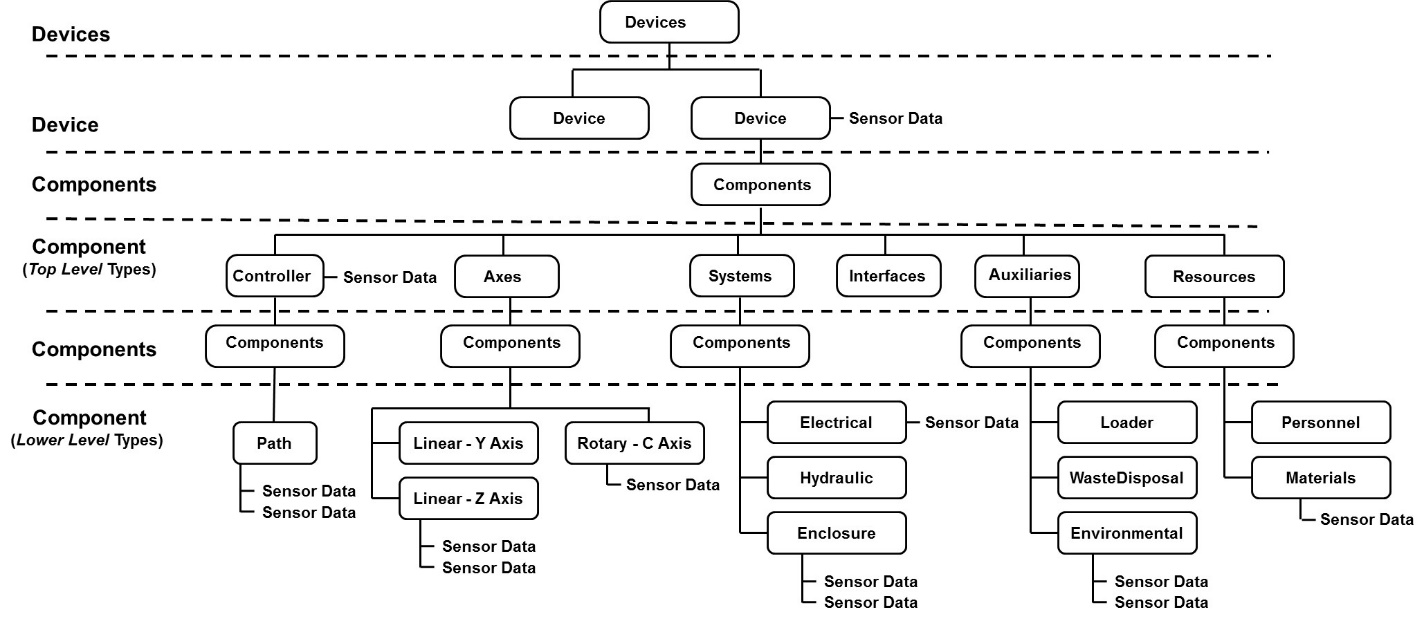
\includegraphics[width=.75\textwidth]{figures/sensor-data-associations.png}
  \caption{Sensor Data Associations}
  \label{fig:sensor-data-associations}
\end{figure}

\subsection{Sensor Unit}
\label{sec:Sensor Unit}

A \gls{sensor unit} is an intelligent piece of equipment that manages the functions of one or more \glspl{sensing element}.

Typical functions of the \gls{sensor unit} include:

\begin{itemize}
\item convert low level signals from the \glspl{sensing element} into data that can be used by other pieces of equipment.  (Example:  Convert a non-linear millivolt signal from a temperature sensor into a scaled temperature value that can be transmitted to another piece of equipment.)

\item process \gls{sensing element} data into calculated values.  (Example:  temperature sensor data is converted into calculated values of average temperature, maximum temperature, minimum temperature, etc.)

\item provide calibration and configuration information associated with each \gls{sensing element}

\item monitor the health and integrity of the \glspl{sensing element} and the \gls{sensor unit}.  (Example:  The \gls{sensor unit} may provide diagnostics on each \gls{sensing element} (e.g., open wire detection) and itself (e.g., measure internal temperature of the \gls{sensor unit}).
\end{itemize}

Depending on how the \gls{sensor unit} is used, it may be considered as either an independent piece of equipment and modeled in the XML document as a \gls{device}, or it may be modeled as a \gls{top level} \gls{component} called \gls{sensor} if it is integral to a piece of equipment.

A \gls{sensor} \may have its own \gls{uuid} so it can be tracked throughout its lifetime.

The following examples demonstrate how a \gls{sensor term} may be modeled in the XML document differently based on how the \gls{sensor term} functions within the overall piece of equipment

Example\#1:   If the \gls{sensor} provides vibration measurement data for the spindle on a piece of equipment, it could be modeled as a \gls{sensor} for rotary axis named C.

\begin{lstlisting}[firstnumber=1,escapechar=|,%
    caption={Example of Sensor for rotary axis}, label={lst:example-of-sensor}]
<Components>
  <Axes
    <Components>
      <Rotary id="c" name="C">
        <Components>
          <Sensor id="spdlm" name="Spindlemonitor">
            <DataItems>
              <DataItem type="DISPLACEMENT" id="cvib"
                category="SAMPLE" name="Svib" 
                units="MILLIMETER"/>
            </DataItems>
          </Sensor >
        <Components>
      </Rotary>
    </Components>
  </Axes>
</Components>
\end{lstlisting}

Example\#2:   If a \gls{sensor} provides measurement data for multiple \gls{component} elements within a piece of equipment and is not associated with any particular \gls{component} element, it \may be modeled in the XML document as an independent \gls{lower level} \gls{component} and the data associated with measurements are associated with their associated \gls{component} elements.

This example represents a \gls{sensor unit} with two \glspl{sensing element}, one measures spindle vibration and the other measures the temperature for the X axis.   The \gls{sensor unit} also has a \gls{sensing element} measuring the internal temperature of the \gls{sensor unit}.

\begin{lstlisting}[firstnumber=1,escapechar=|,%
    caption={Example of Sensor Unit with Sensing Element}, label={lst:example-of-sensor-with-sensing-elements}]
<Device id="d1" uuid="HM1" name="HMC_3Axis">
  <Description>3 Axis Mill</Description>
  <Components>
    <Axes
      <Components>
        <Sensor id="sens1" name="Sensorunit">
          <DataItems>
            <DataItem type="TEMPERATURE" id="sentemp"
              category="SAMPLE" name="Sensortemp" 
              units="DEGREE"/> 
          </DataItems>
        </Sensor >
        <Rotary id="c" name="C">
          <DataItems>
            <DataItem type="DISPLACEMENT" id="cvib"
              %category="SAMPLE" name="Svib" 
              units="MILLIMETER">
                <Source componentid="sens1"/>
            <DataItem/>
          </DataItems>
        </Rotary>
        <Linear id="x" name="X">
          <DataItems>
            <DataItem type="TEMPERATURE" id="xt" 
              category="SAMPLE" name="Xtemp" 
              units="DEGREE">
                <Source componentid="sens1"/>
            <DataItem/>
          </DataItems>
        </Linear>
      <Components>
    </Axes>
  </Components>
</Device>
\end{lstlisting}

\subsection{Sensor Configuration}
\label{sec:Sensor Configuration}

When a \gls{sensor} unit is modeled in the XML document as a \gls{component} or as a separate piece of equipment, it may provide additional configuration information for the \glspl{sensor element} and the \gls{sensor unit} itself.  

\gls{configuration} data provides information required for maintenance and support of the sensor.

\gls{configuration} data is only available when the \gls{sensor} unit is modeled as a \gls{component} or a separate piece of equipment. For details on the modeling of configuration data in the XML document, see \sect{Configuration for Component}.

When \gls{sensor} represents the \gls{sensor unit} for multiple \gls{sensing element}(s), each sensing element is represented by a \gls{channel}.   The \gls{sensor unit} itself and each \gls{channel} representing one \gls{sensing element} \may have its own configuration data.

\gls{sensorconfiguration} can contain any descriptive content for a \gls{sensor unit}.  This element is defined to contain mixed content and additional XML elements (indicated by the \gls{any} element in \fig{sensorconfiguration-schema-diagram}) \may be added to extend the schema for \gls{sensorconfiguration}.

\fig{sensorconfiguration-schema-diagram} represents the structure of the \gls{sensorconfiguration} XML element showing the attributes defined for \gls{sensorconfiguration}. 

\begin{figure}[ht]
  \centering
  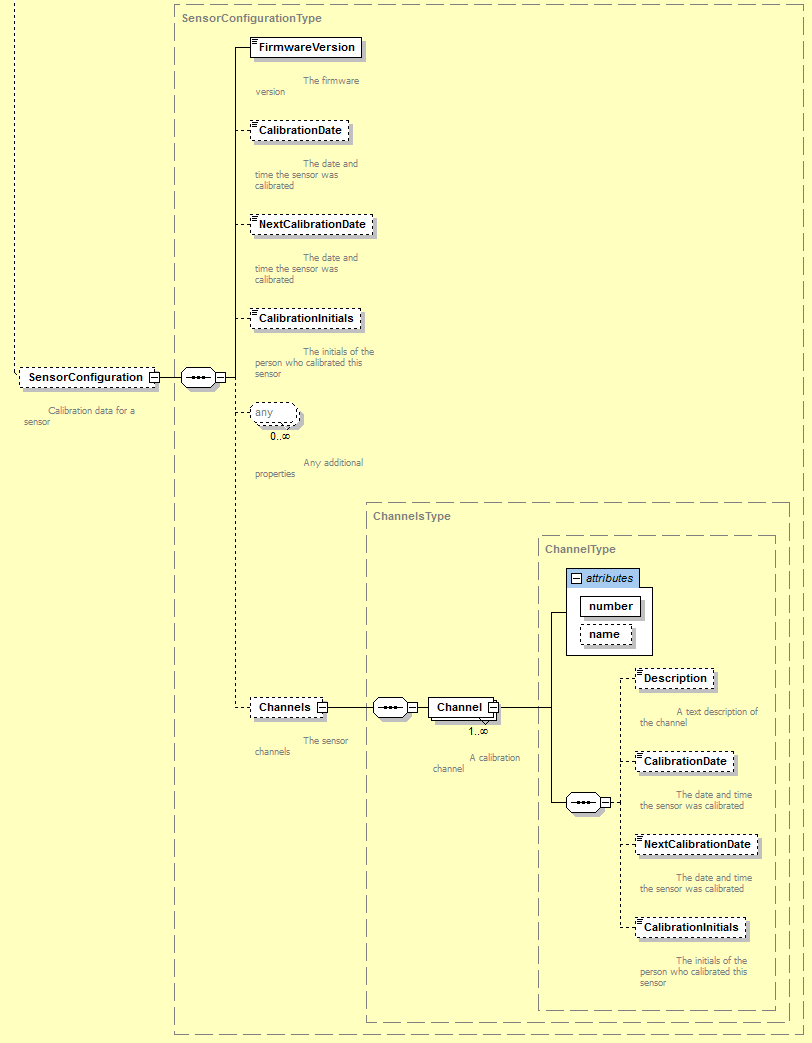
\includegraphics[width=.75\textwidth]{figures/sensorconfiguration-schema-diagram.png}
  \caption{SensorConfiguration Diagram}
  \label{fig:sensorconfiguration-schema-diagram}
\end{figure}
\FloatBarrier

\tabulinesep = 5pt
\begin{longtabu} to \textwidth {
    |l|X[3l]|X[0.75l]|}
\caption{MTConnect SensorConfiguration Element} \label{table:mtconnect-sensorconfiguration-element} \\

\hline
Element & Description & Occurrence \\
\hline
\endfirsthead

\hline
\multicolumn{3}{|c|}{Continuation of Table \ref{table:mtconnect-sensorconfiguration-element}}\\
\hline
Element & Description & Occurrence \\
\hline
\endhead

\gls{sensorconfiguration}
&
An element that can contain descriptive content defining the configuration information for \gls{sensor}.
\newline For \gls{sensor}, the valid configuration is \gls{sensorconfiguration} which provides data from a subset of items commonly found in a transducer electronic data sheet for sensors and actuators called
TEDS.
\newline TEDS formats are defined in IEEE 1451.0 and 1451.4 transducer interface standards (ref 15 and 16, respectively).
\newline MTConnect does not support all of the data represented in the TEDS data, nor does it duplicate the function of the TEDS data sheets. 
&
0..1 \\
\hline


\end{longtabu}


\subsubsection{Elements for SensorConfiguration}

\tbl{elements-for-sensorconfiguration} defines the configuration elements available for \gls{sensorconfiguration}:

\tabulinesep = 5pt
\begin{longtabu} to \textwidth {
    |l|X[3l]|X[0.75l]|}
\caption{Elements for SensorConfiguration} \label{table:elements-for-sensorconfiguration} \\

\hline
Element & Description & Occurrence \\
\hline
\endfirsthead

\hline
\multicolumn{3}{|c|}{Continuation of Table \ref{table:elements-for-sensorconfiguration}}\\
\hline
Element & Description & Occurrence \\
\hline
\endhead

\gls{firmwareversion}
&
\glsentrydesc{firmwareversion}
\newline \gls{firmwareversion} is a required element if \gls{sensorconfiguration} is used.
\newline The data value for \gls{firmwareversion} is provided in the \gls{cdata} for this element and \MAY be any numeric or text
content.
&
1 \\
\hline

\gls{calibrationdate}
&
Date upon which the \gls{sensor unit} was last calibrated.
\newline The data value for \gls{calibrationdate} is provided in the \gls{cdata} for this element and \MUST be represented in the W3C ISO 8601 format.
&
0..1 \\
\hline

\gls{nextcalibrationdate}
&
Date upon which the \gls{sensor unit} is next scheduled to be calibrated.
\newline The data value for \gls{nextcalibrationdate} is provided in the \gls{cdata} for this element and \MUST be represented in the W3C ISO 8601 format.
&
0..1 \\
\hline

\gls{calibrationinitials}
&
\glsentrydesc{calibrationinitials}
\newline The data value for \gls{calibrationinitials} is provided in the \gls{cdata} for this element and \MAY be any numeric or text
content.
&
0..1 \\
\hline

\gls{channels}
&
\glsentrydesc{channels}
&
0..1 \\
\hline

\end{longtabu}

\paragraph{Attributes for Channel}\mbox{}

\gls{channel} represents each \gls{sensing element} connected to a \gls{sensor unit}. \tbl{attributes-for-channel} defines the attributes for \gls{channel}:

\tabulinesep = 5pt
\begin{longtabu} to \textwidth {
    |l|X[3l]|X[0.75l]|}
\caption{Attributes for  Channel} \label{table:attributes-for-channel} \\

\hline
Attribute & Description & Occurrence \\
\hline
\endfirsthead

\hline
\multicolumn{3}{|c|}{Continuation of Table \ref{table:attributes-for-channel}}\\
\hline
Attribute & Description & Occurrence \\
\hline
\endhead

\gls{number} 
&
A unique identifier that will only refer to a specific \gls{sensing element}.
\newline \gls{number} is a required attribute.
\newline For example, this can be the manufacturer code and the serial number.
\newline \gls{number} \SHOULD be alphanumeric and not exceeding 255
characters.
\newline An \gls{nmtoken} XML type.
&
1 \\
\hline

\gls{name}
&
The \gls{name} of the \gls{sensing element}.
\newline \gls{name} is an optional attribute.
\newline \gls{name} \SHOULD be unique within the \gls{sensor unit} to allow for easier data integration. 
\newline An \gls{nmtoken} XML type.
&
0..1 \\
\hline

\end{longtabu}

\paragraph{Elements for Channel}\mbox{}

\tbl{elements-for-channel} describes the elements provided for \gls{channel}.

\tabulinesep = 5pt
\begin{longtabu} to \textwidth {
    |l|X[3l]|X[0.75l]|}
\caption{Elements for Channel} \label{table:elements-for-channel} \\

\hline
Element & Description & Occurrence \\
\hline
\endfirsthead

\hline
\multicolumn{3}{|c|}{Continuation of Table \ref{table:elements-for-channel}}\\
\hline
Element & Description & Occurrence \\
\hline
\endhead

\gls{description}
&
An XML element that can contain any descriptive content.
\newline The \gls{cdata} of \gls{description} \MAY include any additional descriptive information the implementer chooses to include regarding a \gls{sensor element}.

&
0..1 \\
\hline

\gls{calibrationdate}
&
Date upon which the \gls{sensor unit} was last calibrated to the \gls{sensor element}.
\newline The data value for \gls{calibrationdate} is provided in the \gls{cdata} for this element and \MUST be represented in the W3C ISO 8601 format.
&
0..1 \\
\hline

\gls{nextcalibrationdate}
&
Date upon which the \gls{sensor element} is next scheduled to be calibrated with the \gls{sensor unit}.
\newline The data value for \gls{nextcalibrationdate} is provided in the \gls{cdata} for this element and \MUST be represented in the W3C ISO 8601 format.
&
0..1 \\
\hline

\gls{calibrationinitials}
&
\glsentrydesc{calibrationinitials}
\newline The data value for \gls{calibrationinitials} is provided in the \gls{cdata} for this element and \MAY be any numeric or text content.
&
0..1 \\
\hline

\end{longtabu}

\lst{example-of-sensor-configuration-data} is an example of the configuration data for \gls{sensor} that is modeled as a \gls{component}.  It has \gls{configuration} data for the \gls{sensor unit}, one \gls{channel} named A/D:1, and two \gls{dataitems} - \glselementname{voltage sample} (as a \gls{sample category}) and \glselementname{voltage sample} (as a \gls{condition category} or alarm).

\begin{lstlisting}[firstnumber=1,escapechar=|,%
    caption={Example of configuration data for Sensor}, label={lst:example-of-sensor-configuration-data}]
<Sensor id="sensor" name="sensor">
  <Configuration>
    <SensorConfiguration>
      <FirmwareVersion>2.02</FirmwareVersion>
      <CalibrationDate>2010-05-16</CalibrationDate>
      <NextCalibrationDate>2010-05-16</NextCalibrationDate>
      <CalibrationInitials>WS</CalibrationInitials>
      <Channels>
        <Channel number="1" name="A/D:1">
          <Description>A/D With Thermister</Description>
        </Channel>
      </Channels>
    </SensorConfiguration>
  </Configuration>
  <DataItems>
    <DataItem category="CONDITION" id="senvc" 
      type="VOLTAGE" />
    <DataItem category="SAMPLE" id="senv" 
      type="VOLTAGE" units="VOLT" subType="DIRECT" />
  </DataItems>
</Sensor>
\end{lstlisting}




\appendix
\section*{Appendices}
\addcontentsline{toc}{section}{Appendices}
\renewcommand{\thesubsection}{\Alph{subsection}}

\subsection{Bibliography}
\label{Bibliography}

Engineering Industries Association. \textit{EIA Standard - EIA-274-D}, Interchangeable Variable, Block Data Format for Positioning, Contouring, and Contouring/Positioning Numerically Controlled Machines. Washington, D.C. 1979.

ISO TC 184/SC4/WG3 N1089. \textit{ISO/DIS 10303-238:} Industrial automation systems and integration  Product data representation and exchange  Part 238: Application Protocols: Application interpreted model for computerized numerical controllers. Geneva, Switzerland, 2004.

International Organization for Standardization. \textit{ISO 14649:} Industrial automation systems and integration - Physical device control - Data model for computerized numerical controllers - Part 10: General process data. Geneva, Switzerland, 2004.

International Organization for Standardization. \textit{ISO 14649:} Industrial automation systems and integration - Physical device control - Data model for computerized numerical controllers - Part 11: Process data for milling. Geneva, Switzerland, 2000.

International Organization for Standardization. \textit{ISO 6983/1} - Numerical Control of machines - Program format and definition of address words - Part 1: Data format for positioning, line and contouring control systems. Geneva, Switzerland, 1982.

Electronic Industries Association. \textit{ANSI/EIA-494-B-1992}, 32 Bit Binary CL (BCL) and 7 Bit ASCII CL (ACL) Exchange Input Format for Numerically Controlled Machines. Washington, D.C. 1992.

National Aerospace Standard. \textit{Uniform Cutting Tests} - NAS Series: Metal Cutting Equipment Specifications. Washington, D.C. 1969.

International Organization for Standardization. \textit{ISO 10303-11:} 1994, Industrial automation systems and integration  Product data representation and exchange  Part 11: Description methods: The EXPRESS language reference manual. Geneva, Switzerland, 1994.

International Organization for Standardization. \textit{ISO 10303-21:} 1996, Industrial automation systems and integration -- Product data representation and exchange -- Part 21: Implementation methods: Clear text encoding of the exchange structure. Geneva, Switzerland, 1996.

H.L. Horton, F.D. Jones, and E. Oberg. \textit{Machinery's Handbook}. Industrial Press, Inc. New York, 1984.

International Organization for Standardization. \textit{ISO 841-2001:} Industrial automation systems and integration - Numerical control of machines - Coordinate systems and motion nomenclature. Geneva, Switzerland, 2001.

ASME B5.57: \textit{Methods for Performance Evaluation of Computer Numerically Controlled Lathes and Turning Centers}, 1998.

ASME/ANSI B5.54: \textit{Methods for Performance Evaluation of Computer Numerically Controlled Machining Centers}. 2005.

OPC Foundation. \textit{OPC Unified Architecture Specification, Part 1: Concepts Version 1.00}. July 28, 2006.

IEEE STD 1451.0-2007, \textit{Standard for a Smart Transducer Interface for Sensors and Actuators - Common Functions, Communication Protocols, and Transducer Electronic Data Sheet (TEDS) Formats, IEEE Instrumentation and Measurement Society, TC-9, The Institute of Electrical and Electronics Engineers, Inc., New York, N.Y. 10016, SH99684, October 5, 2007.}

IEEE STD 1451.4-1994, Standard for a Smart Transducer Interface for Sensors and Actuators - Mixed-Mode Communication Protocols and Transducer Electronic Data Sheet (TEDS) Formats, IEEE Instrumentation and Measurement Society, TC-9, The Institute of Electrical and Electronics Engineers, Inc., New York, N.Y. 10016, SH95225, December 15, 2004. 

\end{document}
